\documentclass[14pt, a4paper, oneside]{book}

\usepackage[T1]{fontenc}
\usepackage[utf8]{inputenc}
\usepackage[utf8]{vietnam}
\usepackage[vietnam]{babel}

\usepackage[unicode]{hyperref}
\usepackage{amsmath}
\usepackage{amssymb}
\usepackage{eucal}
\usepackage{mathtools}

\usepackage{graphicx}
\graphicspath{ {images/} }

\usepackage{listings}
\lstset{
basicstyle=\ttfamily,
columns=fullflexible,
frame=none,
breaklines=true,
postbreak=\mbox{\textcolor{red}{$\hookrightarrow$}\space},
inputencoding=utf8,
showstringspaces=false
}
\usepackage{courier}
\usepackage{textcomp}
\usepackage{listings}
\usepackage{color}
\definecolor{lbcolor}{rgb}{0.9,0.9,0.9}
\lstset{
literate={-}{-}1,
basicstyle=\fontsize{10}\ttfamily,
columns=fullflexible,
frame=none,
breaklines=true,
postbreak=\mbox{\textcolor{red}{$\hookrightarrow$}\space},
inputencoding=utf8,
upquote=true,
showstringspaces=false,
keepspaces=true,
xleftmargin=.25in,
backgroundcolor=\color{lbcolor},
framexleftmargin=5pt,
framerule=0pt
}
\lstdefinelanguage{JavaScript}{
  keywords={typeof, new, true, false, catch, function, return, null, catch, switch, var, if, in, while, do, else, case, break},
  keywordstyle=\color{black}\bfseries,
  ndkeywords={class, export, boolean, throw, implements, import, this},
  ndkeywordstyle=\color{darkgray}\bfseries,
  identifierstyle=\color{black},
  sensitive=false,
  comment=[l]{//},
  morecomment=[s]{/*}{*/},
  commentstyle=\color{purple}\ttfamily,
  stringstyle=\color{black}\ttfamily,
  morestring=[b]',
  morestring=[b]"
}


\usepackage[makeindex]{imakeidx}
\usepackage[plain]{cite}
\usepackage{natbib}

\hypersetup{
colorlinks=true,
linkcolor=blue,
filecolor=magenta,
urlcolor=cyan,
}

\title{Ghi chú của một coder}
\author{Vũ Anh}
\date{Tháng 01 năm 2018}
%\usepackage{index}
\makeindex

\begin{document}


  \maketitle

  \tableofcontents
  \addcontentsline{toc}{chapter}{\contentsname}
  \chapter{Lập trình là gì?}

\section{Các vấn đề lập trình}

Các vấn đề lập trình với từng ngôn ngữ

\subsection{Nhập môn}

\begin{lstlisting}
code/
├── 1. introduction
├── 2. syntax
├── 3. data structure
├── 4. oop
├── 5. networking
├── 6. os
├── 7. parallel
├── 8. event based
├── 9. error handling
├── 10. logging
├── 11. configuration
├── 12. documentation
├── 13. test
├── 14. ui
├── 15. web
├── 16. database
├── 17. ide
├── 18. package manager
├── 19. build tool
├── 20. make module
└── 21. production (docker)
\end{lstlisting}

\section{Introduction}

Installation (environment, IDE)

Hello world

Courses

Resources


\section{Syntax}

variables and expressions

conditional

loops and Iteration

functions

define, use

parameters

scope of variables

anonymous functions

callbacks

self-invoking functions, inner functions

functions that return functions, functions that redefined themselves

closures

naming convention

comment convention

\section{Cấu trúc dữ liệu}

Number

String

Collection

DateTime

Boolean

Object

\section{Lập trình hướng đối tượng}

Classes & Objects

Inheritance

Encapsulation

Abstraction

Polymorphism

For OOP Example: see Python: OOP

\subsection{Bài tập}

\textbf{Quản lý tài khoản ngân hàng}

\section{Networking}

REST (example with chat app sender, receiver, message)

\subsection{Bài tập}

Guess My Number Game

\section{GUI - Giao diện}

Quản lý hot girl

Quản lý truyện tranh

Create Analog Clock

Chương trình lịch âm dương

Chương trình học từ tiếng Anh

\section{Game}

\begin{itemize}
  \item Create Pong Game
  \item Create flappy bird
  \item Create Bouncing Game
\end{itemize}


\section{Cơ sở dữ liệu}

\subsection{Thử thách}


\section{How to ask a question}

Focus on questions about an actual problem you have faced. Include details about what you have tried and exactly what you are trying to do.

Ask about...

✔ Specific programming problems

✔ Software algorithms

✔ Coding techniques

✔ Software development tools

Not all questions work well in our format. Avoid questions that are primarily opinion-based, or that are likely to generate discussion rather than answers.

Don't ask about...

✖ Questions you haven't tried to find an answer for (show your work!)

✖ Product or service recommendations or comparisons

✖ Requests for lists of things, polls, opinions, discussions, etc.

✖ Anything not directly related to writing computer programs

\section{Các nguyên tắc lập trình}

Generic

KISS (Keep It Simple Stupid)

YAGNI

Do The Simplest Thing That Could Possibly Work

Keep Things DRY

Code For The Maintainer

Avoid Premature Optimization

Inter-Module/Class

Minimise Coupling

Law of Demeter

Composition Over Inheritance

Orthogonality

Module/Class

Maximise Cohesion

Liskov Substitution Principle

Open/Closed Principle

Single Responsibility Principle

Hide Implementation Details

Curly's Law

Software Quality Laws

First Law of Software Quality


\section{Các mô hình lập trình}

Main paradigm approaches 1

1. Imperative


Description:

Computation as statements that directly change a program state (datafields)

Main Characteristics:

Direct assignments, common data structures, global variables

Critics: Edsger W. Dijkstra, Michael A. Jackson

Examples: Assembly, C, C++, Java, PHP, Python

2. Structured

Description:

A style of imperative programming with more logical program structure

Main Characteristics:

Structograms, indentation, either no, or limited use of, goto statements

Examples: C, C++, Java, Python

3. Procedural

Description:

Derived from structured programming, based on the concept of modular programming or the procedure call

Main Characteristics:

Local variables, sequence, selection, iteration, and modularization

Examples: C, C++, Lisp, PHP, Python

4. Functional


Description:

Treats computation as the evaluation of mathematical functions avoiding state and mutable data

Main Characteristics:

Lambda calculus, compositionality, formula, recursion, referential transparency, no side effects

Examples: Clojure, Coffeescript, Elixir, Erlang, F#, Haskell, Lisp, Python, Scala, SequenceL, SML

5. Event-driven including time driven

Description:

Program flow is determined mainly by events, such as mouse clicks or interrupts including timer

Main Characteristics:

Main loop, event handlers, asynchronous processes

Examples: Javascript, ActionScript, Visual Basic

6. Object-oriented

Description:

Treats datafields as objects manipulated through pre-defined methods only

Main Characteristics:

Objects, methods, message passing, information hiding, data abstraction, encapsulation, polymorphism, inheritance, serialization-marshalling

Examples: Common Lisp, C++, C#, Eiffel, Java, PHP, Python, Ruby, Scala

7. Declarative

Description:

Defines computation logic without defining its detailed control flow

Main Characteristics:

4GLs, spreadsheets, report program generators

Examples: SQL, regular expressions, CSS, Prolog

8. Automata-based programming

Description:

Treats programs as a model of a finite state machine or any other formal automata

Main Characteristics:

State enumeration, control variable, state changes, isomorphism, state transition table

Examples: AsmL

\section{Testing}

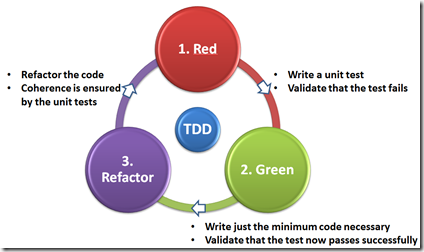
\includegraphics{programming/introduction/unit_test_tdd}

1. Definition 1 2

Test-driven development (TDD) is a software development process that relies on the repetition of a very short development cycle:

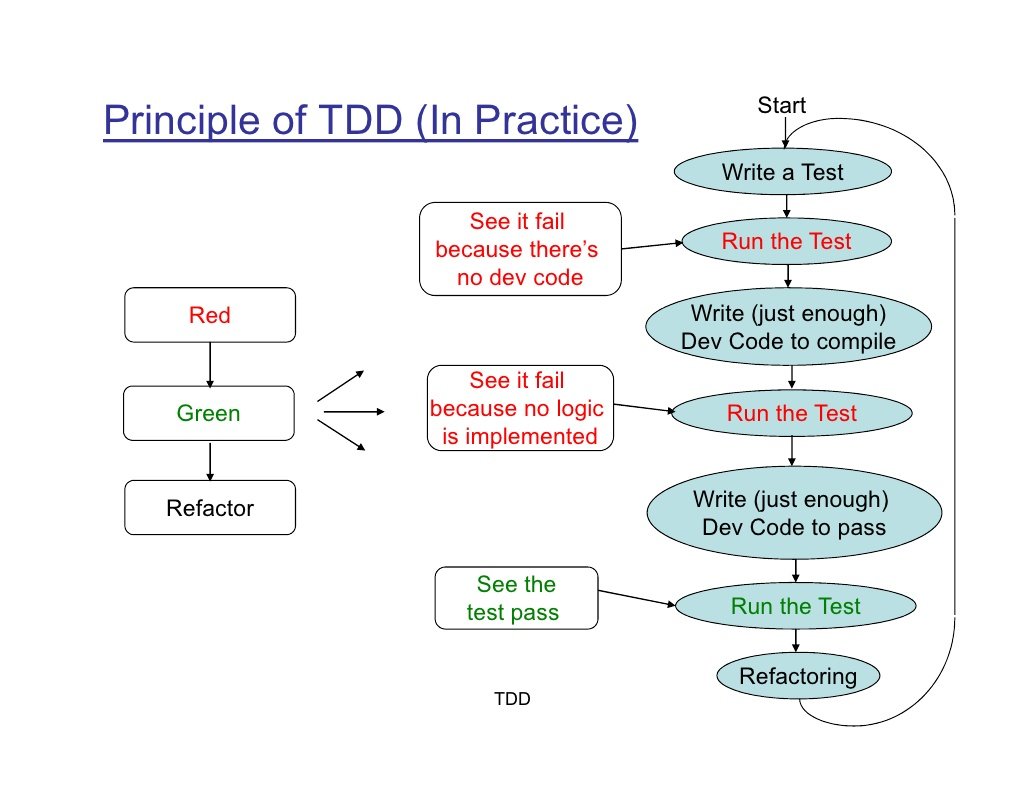
\includegraphics[width=\linewidth]{programming/introduction/tdd.jpg}

Step 1: First the developer writes an (initially failing) automated test case that defines a desired improvement or new function,

Step 2: Then produces the minimum amount of code to pass that test,

Step 3: Finally refactors the new code to acceptable standards.

Kent Beck, who is credited with having developed or 'rediscovered' the technique, stated in 2003 that TDD encourages simple designs and inspires confidence.

2. Principles 2

Kent Beck defines

Never with a single line of code unless you have a failing automated test.
Eliminate duplication
Red: (Automated test fail) Green (Automated test pass because dev code has been written) Refactor (Eliminate duplication, Clean the code)

3. Assertions & Assert Framework

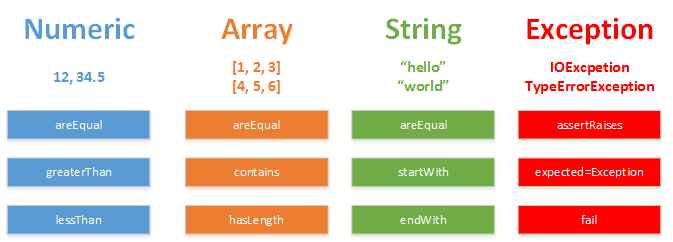
\includegraphics[width=\linewidth]{programming/introduction/tdd_assertion.png}

Assert that the expected results have occurred.
[code lang="java"] @Test public void test() { assertEquals(2, 1 + 1); } [/code]


4. Test Runners 3

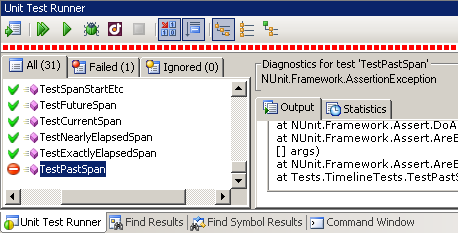
\includegraphics[width=\linewidth]{programming/introduction/tdd_test_runner.png}

When testing a large real-world web app there may be tens or hundreds of test cases, and we certainly don't want to run each one manually. In such as scenario we need to use a test runner to find and execute the tests for us, and in this article we'll explore just that.

A test runner provides the a good basis for a real testing framework. A test runner is designed to run tests, tag tests with attributes (annotations), and provide reporting and other features.

In general you break your tests up into 3 standard sections; setUp(), tests, and tearDown(), typical for a test runner setup.

The setUp() and tearDown() methods are run automatically for every test, and contain respectively:

The setup steps you need to take before running the test, such as unlocking the screen and killing open apps.
The cooldown steps you need to run after the test, such as closing the Marionette session.

5. Test Frameworks

Language	Test Frameworks
C++/VisualStudio	C++: Test
Web Service	rest-assured
Web UI	SeleniumHQ

\section{Logging}

Logging is the process of recording application actions and state to a secondary interface.


\includegraphics[width=\linewidth]{programming/introduction/logging}

Logging System

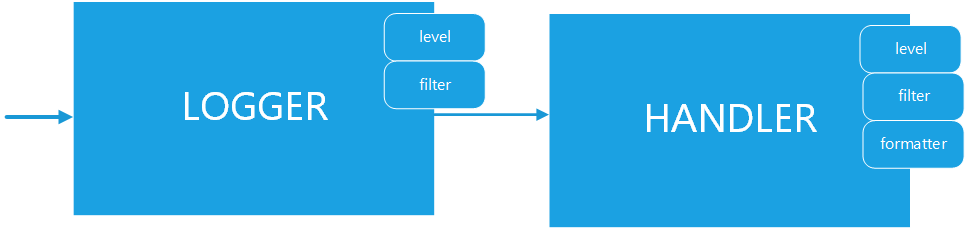
\includegraphics[width=\linewidth]{programming/introduction/logging_system}

Levels

Level	When it’s used
DEBUG	Detailed information, typically of interest only when diagnosing problems.
INFO	Confirmation that things are working as expected.
WARNING	An indication that something unexpected happened, or indicative of some problem in the near future (e.g. ‘disk space low’). The software is still working as expected.

ERROR

Due to a more serious problem, the software has not been able to perform some function.
CRITICAL	A serious error, indicating that the program itself may be unable to continue running.
Best Practices 2 4 5
Logging should always be considered when handling an exception but should never take the place of a real handler.
Keep all logging code in your production code. Have an ability to enable more/less detailed logging in production, preferably per subsystem and without restarting your program.
Make logs easy to parse by grep and by eye. Stick to several common fields at the beginning of each line. Identify time, severity, and subsystem in every line. Clearly formulate the message. Make every log message easy to map to its source code line.
If an error happens, try to collect and log as much information as possible. It may take long but it's OK because normal processing has failed anyway. Not having to wait when the same condition happens in production with a debugger attached is priceless.

\section{Lập trình hàm}

Functional
Without mutable variables, assignment, conditional

Advantages 1
Most functional languages provide a nice, protected environment, somewhat like JavaLanguage. It's good to be able to catch exceptions instead of having CoreDumps in stability-critical applications.
FP encourages safe ways of programming. I've never seen an OffByOne mistake in a functional program, for example... I've seen one. Adding two lengths to get an index but one of them was zero-indexed. Easy to discover though. -- AnonymousDonor
Functional programs tend to be much more terse than their ImperativeLanguage counterparts. Often this leads to enhanced programmer productivity.
FP encourages quick prototyping. As such, I think it is the best software design paradigm for ExtremeProgrammers... but what do I know.
FP is modular in the dimension of functionality, where ObjectOrientedProgramming is modular in the dimension of different components.
Generic routines (also provided by CeePlusPlus) with easy syntax. ParametricPolymorphism
The ability to have your cake and eat it. Imagine you have a complex OO system processing messages - every component might make state changes depending on the message and then forward the message to some objects it has links to. Wouldn't it be just too cool to be able to easily roll back every change if some object deep in the call hierarchy decided the message is flawed? How about having a history of different states?
Many housekeeping tasks made for you: deconstructing data structures (PatternMatching), storing variable bindings (LexicalScope with closures), strong typing (TypeInference), * GarbageCollection, storage allocation, whether to use boxed (pointer-to-value) or unboxed (value directly) representation...
Safe multithreading! Immutable data structures are not subject to data race conditions, and consequently don't have to be protected by locks. If you are always allocating new objects, rather than destructively manipulating existing ones, the locking can be hidden in the allocation and GarbageCollection system.

\section{Lập trình song song}

Paralell/Concurrency Programming
1. Callback Pattern 2
Callback functions are derived from a programming paradigm known as functional programming. At a fundamental level, functional programming specifies the use of functions as arguments. Functional programming was—and still is, though to a much lesser extent today—seen as an esoteric technique of specially trained, master programmers.

Fortunately, the techniques of functional programming have been elucidated so that mere mortals like you and me can understand and use them with ease. One of the chief techniques in functional programming happens to be callback functions. As you will read shortly, implementing callback functions is as easy as passing regular variables as arguments. This technique is so simple that I wonder why it is mostly covered in advanced JavaScript topics.

[code lang="javascript"] function getN(){ return 10; }

var n = getN();

function getAsyncN(callback){ setTimeout(function(){ callback(10); }, 1000); }

function afterGetAsyncN(result){ var n = 10; console.log(n); }

getAsyncN(afterGetAsyncN); [/code]

2. Promise Pattern 1 3
What is a promise?
The core idea behind promises is that a promise represents the result of an asynchronous operation.

A promise is in one of three different states:

pending - The initial state of a promise.
fulfilled - The state of a promise representing a successful operation.
rejected - The state of a promise representing a failed operation.
Once a promise is fulfilled or rejected, it is immutable (i.e. it can never change again).


\begin{lstlisting}[language=Javscript]
function aPromise(message){
  return new Promise(function(fulfill, reject){
    if(message == "success"){
      fulfill("it is a success Promise");
    } if(message == "fail"){
      reject("it is a fail Promise");
    }
  });
}
\end{lstlisting}

Usage:

\begin{lstlisting}[language=Javascript]
aPromise("success").then(function(successMessage){
  console.log(successMessage) }, function(failMessage){
  // it is a success Promise
  console.log(failMessage)
})
\end{lstlisting}

\begin{lstlisting}[language=Javascript]
aPromise("fail").then(function(successMessage){
  console.log(successMessage) }, function(failMessage){
  console.log(failMessage)
}) // it is a fail Promise
\end{lstlisting}

\section{IDE - Môi trường phát triển tích hợp}

An integrated development environment (IDE) is a software application that provides comprehensive facilities to computer programmers for software development. An IDE normally consists of a source code editor, build automation tools and a debugger. Most modern IDEs have intelligent code completion.

1. Navigation

Word Navigation Line Navigation File Navigation

2. Editing

Auto Complete Code Complete Multicursor Template (Snippets)

3. Formatting

Debugging
Custom Rendering for Object
  \part{Lập trình}

\chapter{Lập trình là gì?}

\section{Các vấn đề lập trình}

Các vấn đề lập trình với từng ngôn ngữ

\subsection{Nhập môn}

\begin{lstlisting}
code/
├── 1. introduction
├── 2. syntax
├── 3. data structure
├── 4. oop
├── 5. networking
├── 6. os
├── 7. parallel
├── 8. event based
├── 9. error handling
├── 10. logging
├── 11. configuration
├── 12. documentation
├── 13. test
├── 14. ui
├── 15. web
├── 16. database
├── 17. ide
├── 18. package manager
├── 19. build tool
├── 20. make module
└── 21. production (docker)
\end{lstlisting}

\section{Introduction}

Installation (environment, IDE)

Hello world

Courses

Resources


\section{Syntax}

variables and expressions

conditional

loops and Iteration

functions

define, use

parameters

scope of variables

anonymous functions

callbacks

self-invoking functions, inner functions

functions that return functions, functions that redefined themselves

closures

naming convention

comment convention

\section{Cấu trúc dữ liệu}

Number

String

Collection

DateTime

Boolean

Object

\section{Lập trình hướng đối tượng}

Classes & Objects

Inheritance

Encapsulation

Abstraction

Polymorphism

For OOP Example: see Python: OOP

\subsection{Bài tập}

\textbf{Quản lý tài khoản ngân hàng}

\section{Networking}

REST (example with chat app sender, receiver, message)

\subsection{Bài tập}

Guess My Number Game

\section{GUI - Giao diện}

Quản lý hot girl

Quản lý truyện tranh

Create Analog Clock

Chương trình lịch âm dương

Chương trình học từ tiếng Anh

\section{Game}

\begin{itemize}
  \item Create Pong Game
  \item Create flappy bird
  \item Create Bouncing Game
\end{itemize}


\section{Cơ sở dữ liệu}

\subsection{Thử thách}


\section{How to ask a question}

Focus on questions about an actual problem you have faced. Include details about what you have tried and exactly what you are trying to do.

Ask about...

✔ Specific programming problems

✔ Software algorithms

✔ Coding techniques

✔ Software development tools

Not all questions work well in our format. Avoid questions that are primarily opinion-based, or that are likely to generate discussion rather than answers.

Don't ask about...

✖ Questions you haven't tried to find an answer for (show your work!)

✖ Product or service recommendations or comparisons

✖ Requests for lists of things, polls, opinions, discussions, etc.

✖ Anything not directly related to writing computer programs

\section{Các nguyên tắc lập trình}

Generic

KISS (Keep It Simple Stupid)

YAGNI

Do The Simplest Thing That Could Possibly Work

Keep Things DRY

Code For The Maintainer

Avoid Premature Optimization

Inter-Module/Class

Minimise Coupling

Law of Demeter

Composition Over Inheritance

Orthogonality

Module/Class

Maximise Cohesion

Liskov Substitution Principle

Open/Closed Principle

Single Responsibility Principle

Hide Implementation Details

Curly's Law

Software Quality Laws

First Law of Software Quality


\section{Các mô hình lập trình}

Main paradigm approaches 1

1. Imperative


Description:

Computation as statements that directly change a program state (datafields)

Main Characteristics:

Direct assignments, common data structures, global variables

Critics: Edsger W. Dijkstra, Michael A. Jackson

Examples: Assembly, C, C++, Java, PHP, Python

2. Structured

Description:

A style of imperative programming with more logical program structure

Main Characteristics:

Structograms, indentation, either no, or limited use of, goto statements

Examples: C, C++, Java, Python

3. Procedural

Description:

Derived from structured programming, based on the concept of modular programming or the procedure call

Main Characteristics:

Local variables, sequence, selection, iteration, and modularization

Examples: C, C++, Lisp, PHP, Python

4. Functional


Description:

Treats computation as the evaluation of mathematical functions avoiding state and mutable data

Main Characteristics:

Lambda calculus, compositionality, formula, recursion, referential transparency, no side effects

Examples: Clojure, Coffeescript, Elixir, Erlang, F#, Haskell, Lisp, Python, Scala, SequenceL, SML

5. Event-driven including time driven

Description:

Program flow is determined mainly by events, such as mouse clicks or interrupts including timer

Main Characteristics:

Main loop, event handlers, asynchronous processes

Examples: Javascript, ActionScript, Visual Basic

6. Object-oriented

Description:

Treats datafields as objects manipulated through pre-defined methods only

Main Characteristics:

Objects, methods, message passing, information hiding, data abstraction, encapsulation, polymorphism, inheritance, serialization-marshalling

Examples: Common Lisp, C++, C#, Eiffel, Java, PHP, Python, Ruby, Scala

7. Declarative

Description:

Defines computation logic without defining its detailed control flow

Main Characteristics:

4GLs, spreadsheets, report program generators

Examples: SQL, regular expressions, CSS, Prolog

8. Automata-based programming

Description:

Treats programs as a model of a finite state machine or any other formal automata

Main Characteristics:

State enumeration, control variable, state changes, isomorphism, state transition table

Examples: AsmL

\section{Testing}

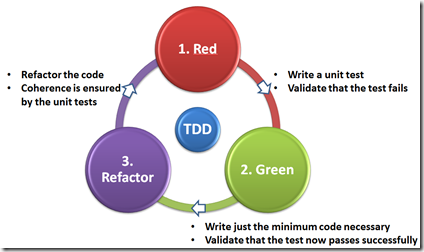
\includegraphics{programming/introduction/unit_test_tdd}

1. Definition 1 2

Test-driven development (TDD) is a software development process that relies on the repetition of a very short development cycle:

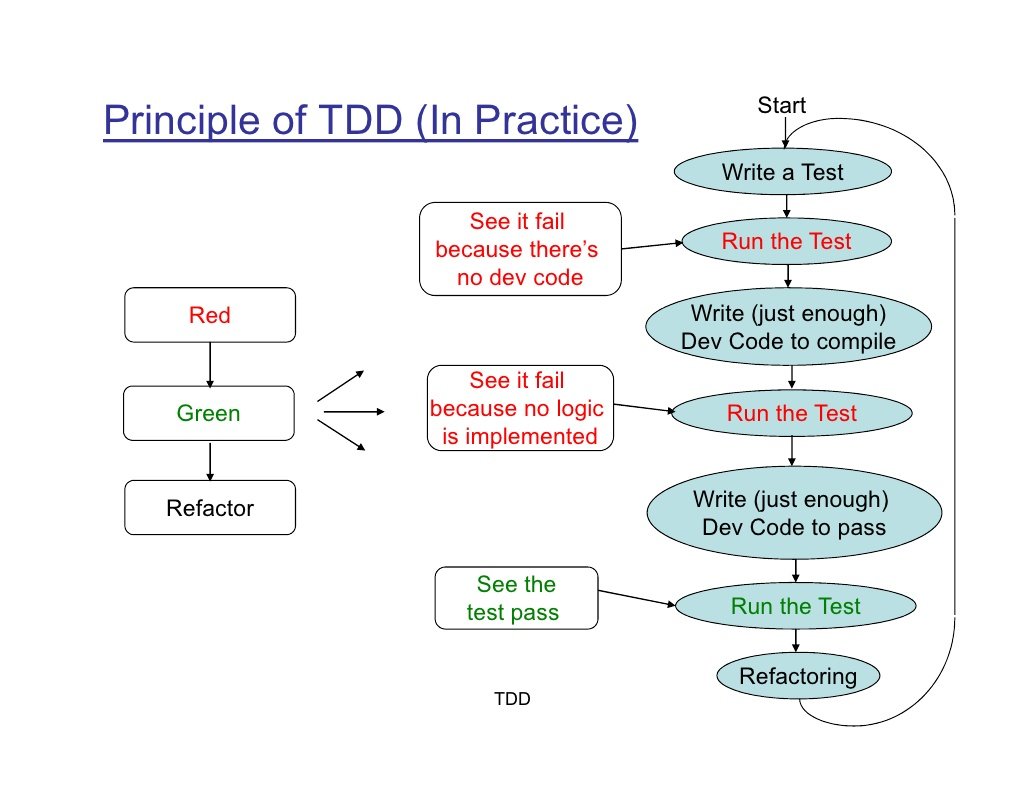
\includegraphics[width=\linewidth]{programming/introduction/tdd.jpg}

Step 1: First the developer writes an (initially failing) automated test case that defines a desired improvement or new function,

Step 2: Then produces the minimum amount of code to pass that test,

Step 3: Finally refactors the new code to acceptable standards.

Kent Beck, who is credited with having developed or 'rediscovered' the technique, stated in 2003 that TDD encourages simple designs and inspires confidence.

2. Principles 2

Kent Beck defines

Never with a single line of code unless you have a failing automated test.
Eliminate duplication
Red: (Automated test fail) Green (Automated test pass because dev code has been written) Refactor (Eliminate duplication, Clean the code)

3. Assertions & Assert Framework

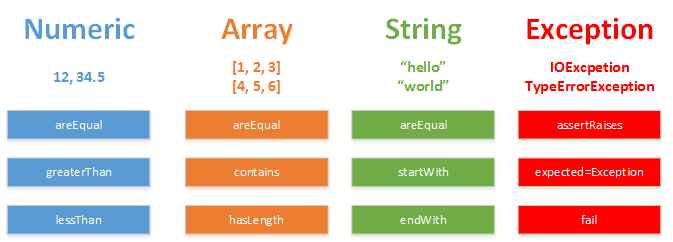
\includegraphics[width=\linewidth]{programming/introduction/tdd_assertion.png}

Assert that the expected results have occurred.
[code lang="java"] @Test public void test() { assertEquals(2, 1 + 1); } [/code]


4. Test Runners 3

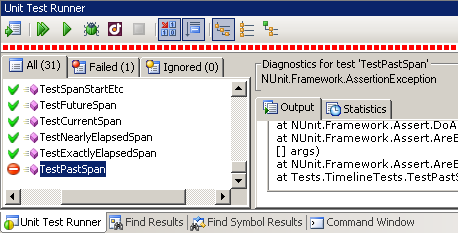
\includegraphics[width=\linewidth]{programming/introduction/tdd_test_runner.png}

When testing a large real-world web app there may be tens or hundreds of test cases, and we certainly don't want to run each one manually. In such as scenario we need to use a test runner to find and execute the tests for us, and in this article we'll explore just that.

A test runner provides the a good basis for a real testing framework. A test runner is designed to run tests, tag tests with attributes (annotations), and provide reporting and other features.

In general you break your tests up into 3 standard sections; setUp(), tests, and tearDown(), typical for a test runner setup.

The setUp() and tearDown() methods are run automatically for every test, and contain respectively:

The setup steps you need to take before running the test, such as unlocking the screen and killing open apps.
The cooldown steps you need to run after the test, such as closing the Marionette session.

5. Test Frameworks

Language	Test Frameworks
C++/VisualStudio	C++: Test
Web Service	rest-assured
Web UI	SeleniumHQ

\section{Logging}

Logging is the process of recording application actions and state to a secondary interface.


\includegraphics[width=\linewidth]{programming/introduction/logging}

Logging System

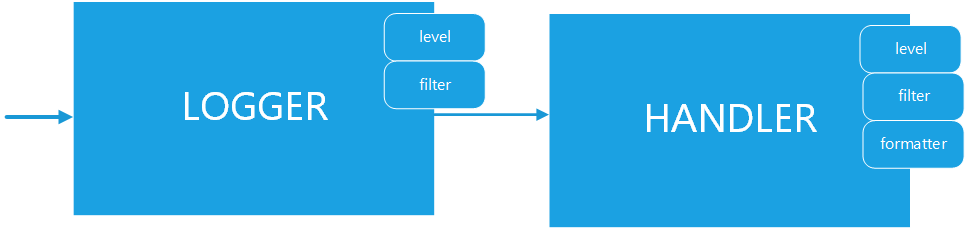
\includegraphics[width=\linewidth]{programming/introduction/logging_system}

Levels

Level	When it’s used
DEBUG	Detailed information, typically of interest only when diagnosing problems.
INFO	Confirmation that things are working as expected.
WARNING	An indication that something unexpected happened, or indicative of some problem in the near future (e.g. ‘disk space low’). The software is still working as expected.

ERROR

Due to a more serious problem, the software has not been able to perform some function.
CRITICAL	A serious error, indicating that the program itself may be unable to continue running.
Best Practices 2 4 5
Logging should always be considered when handling an exception but should never take the place of a real handler.
Keep all logging code in your production code. Have an ability to enable more/less detailed logging in production, preferably per subsystem and without restarting your program.
Make logs easy to parse by grep and by eye. Stick to several common fields at the beginning of each line. Identify time, severity, and subsystem in every line. Clearly formulate the message. Make every log message easy to map to its source code line.
If an error happens, try to collect and log as much information as possible. It may take long but it's OK because normal processing has failed anyway. Not having to wait when the same condition happens in production with a debugger attached is priceless.

\section{Lập trình hàm}

Functional
Without mutable variables, assignment, conditional

Advantages 1
Most functional languages provide a nice, protected environment, somewhat like JavaLanguage. It's good to be able to catch exceptions instead of having CoreDumps in stability-critical applications.
FP encourages safe ways of programming. I've never seen an OffByOne mistake in a functional program, for example... I've seen one. Adding two lengths to get an index but one of them was zero-indexed. Easy to discover though. -- AnonymousDonor
Functional programs tend to be much more terse than their ImperativeLanguage counterparts. Often this leads to enhanced programmer productivity.
FP encourages quick prototyping. As such, I think it is the best software design paradigm for ExtremeProgrammers... but what do I know.
FP is modular in the dimension of functionality, where ObjectOrientedProgramming is modular in the dimension of different components.
Generic routines (also provided by CeePlusPlus) with easy syntax. ParametricPolymorphism
The ability to have your cake and eat it. Imagine you have a complex OO system processing messages - every component might make state changes depending on the message and then forward the message to some objects it has links to. Wouldn't it be just too cool to be able to easily roll back every change if some object deep in the call hierarchy decided the message is flawed? How about having a history of different states?
Many housekeeping tasks made for you: deconstructing data structures (PatternMatching), storing variable bindings (LexicalScope with closures), strong typing (TypeInference), * GarbageCollection, storage allocation, whether to use boxed (pointer-to-value) or unboxed (value directly) representation...
Safe multithreading! Immutable data structures are not subject to data race conditions, and consequently don't have to be protected by locks. If you are always allocating new objects, rather than destructively manipulating existing ones, the locking can be hidden in the allocation and GarbageCollection system.

\section{Lập trình song song}

Paralell/Concurrency Programming
1. Callback Pattern 2
Callback functions are derived from a programming paradigm known as functional programming. At a fundamental level, functional programming specifies the use of functions as arguments. Functional programming was—and still is, though to a much lesser extent today—seen as an esoteric technique of specially trained, master programmers.

Fortunately, the techniques of functional programming have been elucidated so that mere mortals like you and me can understand and use them with ease. One of the chief techniques in functional programming happens to be callback functions. As you will read shortly, implementing callback functions is as easy as passing regular variables as arguments. This technique is so simple that I wonder why it is mostly covered in advanced JavaScript topics.

[code lang="javascript"] function getN(){ return 10; }

var n = getN();

function getAsyncN(callback){ setTimeout(function(){ callback(10); }, 1000); }

function afterGetAsyncN(result){ var n = 10; console.log(n); }

getAsyncN(afterGetAsyncN); [/code]

2. Promise Pattern 1 3
What is a promise?
The core idea behind promises is that a promise represents the result of an asynchronous operation.

A promise is in one of three different states:

pending - The initial state of a promise.
fulfilled - The state of a promise representing a successful operation.
rejected - The state of a promise representing a failed operation.
Once a promise is fulfilled or rejected, it is immutable (i.e. it can never change again).


\begin{lstlisting}[language=Javscript]
function aPromise(message){
  return new Promise(function(fulfill, reject){
    if(message == "success"){
      fulfill("it is a success Promise");
    } if(message == "fail"){
      reject("it is a fail Promise");
    }
  });
}
\end{lstlisting}

Usage:

\begin{lstlisting}[language=Javascript]
aPromise("success").then(function(successMessage){
  console.log(successMessage) }, function(failMessage){
  // it is a success Promise
  console.log(failMessage)
})
\end{lstlisting}

\begin{lstlisting}[language=Javascript]
aPromise("fail").then(function(successMessage){
  console.log(successMessage) }, function(failMessage){
  console.log(failMessage)
}) // it is a fail Promise
\end{lstlisting}

\section{IDE - Môi trường phát triển tích hợp}

An integrated development environment (IDE) is a software application that provides comprehensive facilities to computer programmers for software development. An IDE normally consists of a source code editor, build automation tools and a debugger. Most modern IDEs have intelligent code completion.

1. Navigation

Word Navigation Line Navigation File Navigation

2. Editing

Auto Complete Code Complete Multicursor Template (Snippets)

3. Formatting

Debugging
Custom Rendering for Object
\chapter{Python}

\diary{01/11/2017 Thích python vì nó quá đơn giản (và quá đẹp).}

Hướng dẫn online tại \href{http://magizbox.com/training/python/site/}{http://magizbox.com/training/python/site/}

\section{Khóa học 1: Nhập môn Python}

\subsection{Mục tiêu của khóa học}

Ưu điểm của khóa học

\begin{itemize}
  \item Dành cho người mới bắt đầu, chưa từng học lập trình hoặc cho những ai muốn ôn lại kiến thức căn bản về lập trình python.
  \item Dễ học, dễ thực hành, ví dụ trực quan thú vị, không yêu cầu cao về máy móc hay phần mềm đi kèm.
  \item Ví dụ mẫu nhiều, trực quan, thú vị.
\end{itemize}

Kết thúc khóa học bạn sẽ học được gì?

\begin{itemize}
  \item Xây dựng 5 dự án đơn giản với Python 3
\end{itemize}

Với những kiến thức bạn có thể làm gì?

\begin{itemize}
  \item Lập trình viên Python tại các công ty phần mềm
\end{itemize}

\subsection{Đối tượng học viên}

\begin{itemize}
  \item Những bạn chưa từng lập trình
  \item Những bạn đã có kinh nghiệm lập trình nhưng chưa lập trình python
\end{itemize}

\section{Giới thiệu}

\textbf{Python} is a general-purpose interpreted, interactive, object-oriented, and high-level programming language. It was created by Guido van Rossum during 1985- 1990. Like Perl, Python source code is also available under the GNU General Public License (GPL). This tutorial gives enough understanding on Python programming language.

\textbf{Python is Interpreted}: Python is processed at runtime by the interpreter. You do not need to compile your program before executing it. This is similar to PERL and PHP.

\textbf{Python is Interactive}: You can actually sit at a Python prompt and interact with the interpreter directly to write your programs.

\textbf{Python is Object-Oriented}: Python supports Object-Oriented style or technique of programming that encapsulates code within objects.

\textbf{Python is Beginner Friendly}: Python is a great language for the beginner-level programmers and supports the development of a wide range of applications from simple text processing to WWW browsers to games.

\textbf{Sách}

\href{https://docs.google.com/document/d/1gQFMXZtynpuTenoOQNGCHttArT4NspTWcyJQr5ps9Mk/edit?usp=sharing}{Tập hợp các sách python}

\textbf{Khoá học}

\href{1frO9QYhgsXbMzcyXoA4czWkxTWF8RBTJVf9uoO1rElU}{Tập hợp các khóa học python}

\textbf{Tham khảo}

\href{http://blog.tryolabs.com/2015/12/15/top-10-python-libraries-of-2015/}{Top 10 Python Libraries Of 2015}

\section{Cài đặt}

\subsection{Trên Windows}

\textbf{Anaconda 4.3.0}

Anaconda is BSD licensed which gives you permission to use Anaconda commercially and for redistribution.

1. Download the installer

2. Optional: Verify data integrity with MD5 or SHA-256
3. Double-click the .exe file to install Anaconda and follow the instructions on the screen

Python 3.6 version
64-BIT INSTALLER
Python 2.7 version
64-BIT INSTALLER
Step 2. Discover the Map

https://docs.python.org/2/library/index.html

\subsection{Trên CentOS}

Developer tools

The Development tools will allow you to build and compile software from source code. Tools for building RPMs are also included, as well as source code management tools like Git, SVN, and CVS.

\begin{lstlisting}[language=bash]
yum groupinstall "Development tools"
yum install zlib-devel
yum install bzip2-devel
yum install openssl-devel
yum install ncurses-devel
yum install sqlite-devel
\end{lstlisting}

Python & Anaconda
Anaconda is BSD licensed which gives you permission to use Anaconda commercially and for redistribution.

\begin{lstlisting}[language=bash]
cd /opt
wget --no-check-certificate https://www.python.org/ftp/python/2.7.6/Python-2.7.6.tar.xz
tar xf Python-2.7.6.tar.xz
cd Python-2.7.6
./configure --prefix=/usr/local
make && make altinstall
## link
ln -s /usr/local/bin/python2.7 /usr/local/bin/python
# final check
which python
python -V
# install Anaconda
cd ~/Downloads
wget https://repo.continuum.io/archive/Anaconda-2.3.0-Linux-x86_64.sh
bash ~/Downloads/Anaconda-2.3.0-Linux-x86_64.sh
\end{lstlisting}

\section{Biến - Hộp nhỏ}

\section{123s - Số trong Python}

\subsection{Print, print}

\begin{lstlisting}[language=python]
print "Hello World"
\end{lstlisting}

\subsection{Conditional}

\begin{lstlisting}[language=Python]
if you_smart:
    print "learn python"
else:
    print "go away"
\end{lstlisting}

\subsection{Loop}

In general, statements are executed sequentially: The first statement in a function is executed first, followed by the second, and so on. There may be a situation when you need to execute a block of code several number of times.

Programming languages provide various control structures that allow for more complicated execution paths. A loop statement allows us to execute a statement or group of statements multiple times. The following diagram illustrates a loop statement


Python programming language provides following types of loops to handle looping requirements.

while loop	Repeats a statement or group of statements while a given condition is TRUE. It tests the condition before executing the loop body.
for loop	Executes a sequence of statements multiple times and abbreviates the code that manages the loop variable.
nested loops	You can use one or more loop inside any another while, for or do..while loop.

\subsection{While Loop}

A while loop statement in Python programming language repeatedly executes a target statement as long as a given condition is true.

Syntax

The syntax of a while loop in Python programming language is

\begin{lstlisting}[language=Python]
while expression:
   statement(s)
\end{lstlisting}

Example

\begin{lstlisting}[language=Python]
count = 0
while count < 9:
   print 'The count is:', count
   count += 1
print "Good bye!"
\end{lstlisting}


\subsection{For Loop}

It has the ability to iterate over the items of any sequence, such as a list or a string.

Syntax

\begin{lstlisting}[language=Python]
for iterating_var in sequence:
   statements(s)
\end{lstlisting}

If a sequence contains an expression list, it is evaluated first. Then, the first item in the sequence is assigned to the iterating variable iterating_var. Next, the statements block is executed. Each item in the list is assigned to iterating_var, and the statement(s) block is executed until the entire sequence is exhausted.

Example

\begin{lstlisting}[language=Python]
for i in range(10):
    print "hello", i

for letter in 'Python':
   print 'Current letter :', letter

fruits = ['banana', 'apple',  'mango']
for fruit in fruits:
   print 'Current fruit :', fruit

print "Good bye!"
\end{lstlisting}

Yield and Generator

Yield is a keyword that is used like return, except the function will return a generator.

\begin{lstlisting}[language=Python]
def createGenerator():
    yield 1
    yield 2
    yield 3
mygenerator = createGenerator() # create a generator
print(mygenerator) # mygenerator is an object!
# <generator object createGenerator at 0xb7555c34>
for i in mygenerator:
    print(i)
# 1
# 2
# 3
\end{lstlisting}


Visit Yield and Generator explained for more information

Functions

Variable-length arguments

\begin{lstlisting}[language=Python]
def functionname([formal_args,] *var_args_tuple ):
   "function_docstring"
   function_suite
   return [expression]
\end{lstlisting}

Example

\begin{lstlisting}[language=Python]
#!/usr/bin/python

# Function definition is here
def printinfo( arg1, *vartuple ):
   "This prints a variable passed arguments"
   print "Output is: "
   print arg1
   for var in vartuple:
      print var
   return;

# Now you can call printinfo function
printinfo( 10 )
printinfo( 70, 60, 50 )
\end{lstlisting}

Coding Convention
Code layout
Indentation: 4 spaces

Suggest Readings

"Python Functions". www.tutorialspoint.com
"Python Loops". www.tutorialspoint.com
"What does the “yield” keyword do?". stackoverflow.com
"Improve Your Python: 'yield' and Generators Explained". jeffknupp.com

\textbf{Vấn đề với mảng}

\begin{item}
  \item Random Sampling \footnote{tham khảo [pytorch](http://pytorch.org/docs/master/torch.html?highlight=randn#torch.randn), [numpy](https://docs.scipy.org/doc/numpy-1.13.0/reference/routines.random.html))} - sinh ra một mảng ngẫu nhiên trong khoảng (0, 1), mảng ngẫu nhiên số nguyên trong khoảng (x, y), mảng ngẫu nhiên là permutation của số từ 1 đến n
\end{item}

\section{Cấu trúc dữ liệu}

\subsection{Number}

Basic Operation

\begin{lstlisting}[language=Python]
1
1.2
1 + 2
abs(-5)
\end{lstlisting}

\subsection{Collection}

In this post I will cover 4 most popular data types in python list, tuple, set, dictionary

List
The most basic data structure in Python is the sequence. Each element of a sequence is assigned a number - its position or index. The first index is zero, the second index is one, and so forth.

The list is a most versatile datatype available in Python which can be written as a list of comma-separated values (items) between square brackets. Important thing about a list is that items in a list need not be of the same type.

Usage

A list keeps order, dict and set don't: when you care about order, therefore, you must use list (if your choice of containers is limited to these three, of course)
Most Popular Operations

Create a list
a = ["a", "b", 3]
Access values in list
a[1]
Updated List
a[0] = 5
Delete list elements
del a[1]
Reverse a list
a[::-1]
Itertools
[a + b for (a, b) in itertools.product(x, y)]
Select random elements in list
random.choice(x)
random.sample(x, 3)
Create a list
a = [1, 2, 3]
# [1, 2, 3]
Access values in list
list1 = ['physics', 'chemistry', 1997, 2000]
list2 = [1, 2, 3, 4, 5, 6, 7 ]

print list1[0]   # physics

print list2[1:5] # [2, 3, 4, 5]
Updated lists
list = ['physics', 'chemistry', 1997, 2000]
print list[2] # 1997

list[2] = 2001
print list[2] # 2001
Delete list elements
list1 = ['physics', 'chemistry', 1997, 2000];

print list1
# ['physics', 'chemistry', 1997, 2000]

del list1[2]

print list1
# ['physics', 'chemistry', 2000]
Reverse a list
[1, 3, 2][::-1]
# [2, 3, 1]
Itertools
import itertools

x = [1, 2, 3]
y = [2, 4, 5]

[a + b for (a, b) in itertools.product(x, y)]
# [3, 5, 6, 4, 6, 7, 5, 7, 8]
Select random elements in list
import random

x = [13, 23, 14, 52, 6, 23]

random.choice(x) # 52

random.sample(x, 3) # [23, 14, 52]
Tuples
A tuple is a sequence of immutable Python objects. Tuples are sequences, just like lists. The differences between tuples and lists are, the tuples cannot be changed unlike lists and tuples use parentheses, whereas lists use square brackets.

Usage

Tuples have structure, lists have order
Tuples being immutable there is also a semantic distinction that should guide their usage. Tuples are heterogeneous data structures (i.e., their entries have different meanings), while lists are homogeneous sequences
Most Popular Operations

Create a tuple
t = ("a", 1, 2)
Accessing Values in Tuples
t[0], t[1:]
Updating Tuples
Not allowed
Create a tuple
tup1 = ('physics', 'chemistry', 1997, 2000);
tup2 = (1, 2, 3, 4, 5 );
tup3 = "a", "b", "c", "d";
tup4 = ()
tup5 = (50, )
Accessing Values in Tuples
#!/usr/bin/python

tup1 = ('physics', 'chemistry', 1997, 2000);
tup2 = (1, 2, 3, 4, 5, 6, 7 );

tup1[0]
# physics

tup2[1:5]
[2, 3, 4, 5]
Updating Tuples
Tuples are immutable which means you cannot update or change the values of tuple elements. You are able to take portions of existing tuples to create new tuples as the following example demonstrates

tup1 = (12, 34.56);
tup2 = ('abc', 'xyz');

# Following action is not valid for tuples
# tup1[0] = 100;

# So let's create a new tuple as follows
tup3 = tup1 + tup2;
print tup3
Set
Sets are lists with no duplicate entries.

The sets module provides classes for constructing and manipulating unordered collections of unique elements. Common uses include membership testing, removing duplicates from a sequence, and computing standard math operations on sets such as intersection, union, difference, and symmetric difference.

Usage

set forbids duplicates, list does not: also a crucial distinction.
Most Popular Operations

Create a set
x = set(["Postcard", "Radio", "Telegram"])
Add elements to a set
x.add("Mobile")
Remove elements to a set
x.remove("Radio")
Subset
y.issubset(x)
Intersection
x.intersection(y)
Difference between two sets
x.difference(y)
Create a set
x = set(["Postcard", "Radio", "Telegram"])
x
# set(['Postcard', 'Telegram', 'Radio'])
Add elements to a set
x = set(["Postcard", "Radio", "Telegram"])
x.add("Mobile")
x
# set(['Postcard', 'Telegram', 'Mobile', 'Radio'])
Remove elements to a set
x = set(["Postcard", "Radio", "Telegram"])
x.remove("Radio")
x
# set(['Postcard', 'Telegram'])
Subset
x = set(["a","b","c","d"])
y = set(["c","d"])
y.issubset(x)
# True
Intersection
x = set(["a","b","c","d"])
y = set(["c","d"])
x.intersection(y)
# set(['c', 'd'])
Difference between two sets
x = set(["Postcard", "Radio", "Telegram"])
y = set(["Radio","Television"])
x.difference(y)
# set(['Postcard', 'Telegram'])
Dictionary
Each key is separated from its value by a colon (:), the items are separated by commas, and the whole thing is enclosed in curly braces. An empty dictionary without any items is written with just two curly braces, like this: {}.

Keys are unique within a dictionary while values may not be. The values of a dictionary can be of any type, but the keys must be of an immutable data type such as strings, numbers, or tuples.

Usage

dict associates with each key a value, while list and set just contain values: very different use cases, obviously.
Most Popular Operations

Create a dictionary
d = {"a": 1, "b": 2, "c": 3}
Update dictionary
d["a"] = 4
Delete dictionary elements
del d["a"]
Create a dictionary
dict = {'Name': 'Zara', 'Age': 7, 'Class': 'First'}

print "dict['Name']: ", dict['Name']
print "dict['Age']: ", dict['Age']
Update dictionary
dict = {'Name': 'Zara', 'Age': 7, 'Class': 'First'}

dict['Age'] = 8; # update existing entry
dict['School'] = "DPS School"; # Add new entry


print "dict['Age']: ", dict['Age']
print "dict['School']: ", dict['School']
Delete dictionary elements
dict = {'Name': 'Zara', 'Age': 7, 'Class': 'First'}

del dict['Name']; # remove entry with key 'Name'
dict.clear();     # remove all entries in dict
del dict ;        # delete entire dictionary

print "dict['Age']: ", dict['Age']
print "dict['School']: ", dict['School']
Related Readings
Python Lists, tutorialspoint.com
Python Dictionary, tutorialspoint.com
Python Dictionary Methods, guru99
In Python, when to use a Dictionary, List or Set?, stackoverflow
What's the difference between lists and tuples?, stackoverflow

\subsection{String}

Format
'{0}, {1}, {2}'.format('a', 'b', 'c')
# 'a, b, c'
Regular Expressions
The aim of this chapter of our Python tutorial is to present a detailed led and descriptive introduction into regular expressions. This introduction will explain the theoretical aspects of regular expressions and will show you how to use them in Python scripts.

Regular Expressions are used in programming languages to filter texts or textstrings. It's possible to check, if a text or a string matches a regular expression.

There is an aspect of regular expressions which shouldn't go unmentioned: The syntax of regular expressions is the same for all programming and script languages, e.g. Python, Perl, Java, SED, AWK and even X#.

Functions
match function
This function attempts to match RE pattern to string with optional flags.

re.match(pattern, string, flags=0)
Example

import re

line = "Cats are smarter than dogs"

matched_object = re.match(r'(.*) are (.*?) .*', line, re.M | re.I)

if matched_object:
    print "matched_object.group()  : ", matched_object.group()
    print "matched_object.group(1) : ", matched_object.group(1)
    print "matched_object.group(2) : ", matched_object.group(2)
else:
    print "No match!!"
When the code is executed, it produces following results

matched_object.group()  :  Cats are smarter than dogs
matched_object.group(1) :  Cats
matched_object.group(2) :  smarter
search function
This function searches for first occurrence of RE pattern within stirng with optional flags

re.search(pattern, string, flags=0)
Example

#!/usr/bin/python
import re

line = "Cats are smarter than dogs"

search_object = re.search(r'dogs', line, re.M | re.I)
if search_object:
    print "search --> search_object.group() : ", search_object.group()
else:
    print "Nothing found!!"
When the code is executed, it produces following results

search --> search_object.group() :  dogs
sub function
This method replaces all occurrences of the RE pattern in string with repl, substituting all occurrences unless max provided. This method returns modified string.

re.sub(pattern, repl, string, max=0)
Example

#!/usr/bin/python
import re

phone = "2004-959-559 # This is Phone Number"

# Delete Python-style comments
num = re.sub(r'#.*$', "", phone)
print "Phone Num : ", num

# Remove anything other than digits
num = re.sub(r'\D', "", phone)
print "Phone Num : ", num
When the code is executed, it produces following results

Phone Num :  2004-959-559
Phone Num :  2004959559
Tokens Cheatsheet
Character Classes
.	any character except newline
/go.gle/
google goggle gogle
\w \d \s	word, digit, whitespace
/\w/
AaYyz09 ?!
/\d/
012345 aZ?
/\s/
0123456789 abcd?/
\W \D \S	not word, digit, whitespace
/\W/
abcded   1234 ?>
/\D/
abc 12345 ?<.
/\S/
abc   123?  <.
[abc]	any of a, b or c
/analy[sz]e/
analyse analyze analyxe
[^abc]	not a, b or c
/analy[^sz]e/
analyse analyze analyxe
[a-g]	character between a & g
/[2-4]/
demo1 demo2 demo3 demo4 demo5
Quantifiers & Alternation
a* a+ a?	0 or more, 1 or more, 0 or 1
/go*gle/
gogle gogle google gooooogle hgle
/go+gle/
ggle gogle google gooooogle hgle
/go?gle/
ggle gogle google gooooogle hgle
a{5}, a{2,}	exactly five, two or more
/go{5}gle/
gogle gogle google gooooogle hgle
/go{2,}gle/
gogle gogle google gooooogle hgle
a{1,3}	between one & three
/go{1,3}gle/
gogle gogle google gooogle gooooogle hgle
a+? a{2,}?	match as few as possible
/a+?/
a aa aaaaaa
/a{2,}?/
a aa aaaaaa
ab|cd	match ab or cd
/demo|example/
demo example example1
Anchors
^abc$	start / end of the string
/^abc$/
abc
/^abc/
abc abc
/abc$/
abc abc
\b \B	word, not-word boundary
/\bis\b/
This island is beautiful.
/\Bcat\B/
cat certificate
Escaped characters
\. \* \\	escaped special characters
/\./
username@exampe.com 300.000 USD
/\*/
abc@&%$*123
/\\/
abc@&%$\\123
\t \n \r	tab, linefeed, carriage return
/\t/
abc	def
/ab\n/
ab
/\r/
abc@&%$\\123
\u00A9	unicode escaped ©
/\u00A9/
Copyright©2017 - All rights reserved
Groups and Lockaround
(abc)	capture group
/(demo|example)[0-9]/
demo1example4demo
\1	backreference to group #1
/(abc|def)=\1/
abc=abc def=defabc=def
(?:abc)	non-capturing group
/(?:abc){3}/
abcabcabc abcabc
(?=abc)	positive lookahead
/t(?=s)/
tttssstttss
(?!abc)	negative lookahead
/t(?!s)/
tttssstttss
(?<=abc)	positive lookbehind
/(?<=foo)bar/
foobar fuubar
(?<!abc)	negative lookbehind
/(?<!foo)bar/
foobar fuubar
Related Readings

Online regex tester and debugger: PHP, PCRE, Python, Golang and JavaScript, regex101.com
RegExr: Learn, Build, & Test RegEx, regexr.com

\subsection{Datetime}

Print current time

from datetime import datetime
datetime.now().strftime('%Y-%m-%d %H:%M:%S')
# '2015-12-29 14:02:27'
Get current time

import datetime
datetime.datetime.now()
# datetime(2009, 1, 6, 15, 8, 24, 78915)
Unixtime

import time
int(time.time())
Measure time elapsed

import time

start = time.time()
print("hello")
end = time.time()
print(end - start)
Moment
Dealing with dates in Python shouldn't have to suck.

Installation

pip install moment
Usage

import moment
from datetime import datetime

# Create a moment from a string
moment.date("12-18-2012")

# Create a moment with a specified strftime format
moment.date("12-18-2012", "%m-%d-%Y")

# Moment uses the awesome dateparser library behind the scenes
moment.date("2012-12-18")

# Create a moment with words in it
moment.date("December 18, 2012")

# Create a moment that would normally be pretty hard to do
moment.date("2 weeks ago")

# Create a future moment that would otherwise be really difficult
moment.date("2 weeks from now")

# Create a moment from the current datetime
moment.now()

# The moment can also be UTC-based
moment.utcnow()

# Create a moment with the UTC time zone
moment.utc("2012-12-18")

# Create a moment from a Unix timestamp
moment.unix(1355875153626)

# Create a moment from a Unix UTC timestamp
moment.unix(1355875153626, utc=True)

# Return a datetime instance
moment.date(2012, 12, 18).date

# We can do the same thing with the UTC method
moment.utc(2012, 12, 18).date

# Create and format a moment using Moment.js semantics
moment.now().format("YYYY-M-D")

# Create and format a moment with strftime semantics
moment.date(2012, 12, 18).strftime("%Y-%m-%d")

# Update your moment's time zone
moment.date(datetime(2012, 12, 18)).locale("US/Central").date

# Alter the moment's UTC time zone to a different time zone
moment.utcnow().timezone("US/Eastern").date

# Set and update your moment's time zone. For instance, I'm on the
# west coast, but want NYC's current time.
moment.now().locale("US/Pacific").timezone("US/Eastern")

# In order to manipulate time zones, a locale must always be set or
# you must be using UTC.
moment.utcnow().timezone("US/Eastern").date

# You can also clone a moment, so the original stays unaltered
now = moment.utcnow().timezone("US/Pacific")
future = now.clone().add(weeks=2)
Related Readings
How to get current time in Python, stackoverflow
Does Python's time.time() return the local or UTC timestamp?, stackoverflow
Measure time elapsed in Python?, stackoverflow
momnet, https://github.com/zachwill/moment

\subsection{Object}

Convert dict to object
Elegant way to convert a normal Python dict with some nested dicts to an object

class Struct:
    def __init__(self, **entries):
        self.__dict__.update(entries)
Then, you can use

> args = {'a': 1, 'b': 2}
> s = Struct(**args)
> s
< __main__.Struct instance at 0x01D6A738 >
> s.a
1
> s.b
2
Related Readings

stackoverflow, Convert Python dict to object?

\section{Lập trình hướng đối tượng}

Object Oriented Programming
Python has been an object-oriented language since it existed. Because of this, creating and using classes and objects are downright easy. This chapter helps you become an expert in using Python's object-oriented programming support.

If you do not have any previous experience with object-oriented (OO) programming, you may want to consult an introductory course on it or at least a tutorial of some sort so that you have a grasp of the basic concepts.

\subsection{Classes and Objects}

Classes can be thought of as blueprints for creating objects. When I define a BankAccount class using the class keyword, I haven't actually created a bank account. Instead, what I've created is a sort of instruction manual for constructing "bank account" objects. Let's look at the following example code:

\begin{lstlisting}[language=Python]
class BankAccount:
    id = None
    balance = 0

    def __init__(self, id, balance=0):
        self.id = id
        self.balance = balance

    def __get_balance(self):
        return self.balance

    def withdraw(self, amount):
        self.balance = self.balance - amount

    def deposit(self, amount):
        self.balance = self.balance + amount

john = BankAccount(1, 1000.0)
john.withdraw(100.0)
\end{lstlisting}

The class BankAccount line does not create a new bank account. That is, just because we've defined a BankAcount doesn't mean we've created on; we've merely outlined the blueprint to create a BankAccount object. To do so, we call the class's __init__ method with the proper number of arguments (minus self, which we'll get to in a moment)

So, to use the "blueprint" that we crated by defining the class BankAccount (which is used to create BankAccount objects), we call the class name almost as if it were a function: john = BankAccount(1, 1000.0). This line simple say "use the BankAccount blueprint to create me a new object, which I'll refer to as john".

The john object, known as an instance, is the realized version of the BankAccount class. Before we called BankAccount(), no BankAccount object existed. We can, of course, create as many BankAccount objects as we'd like. There is still, however, only one BankAccount class, regardless of how many instances of the class we create.

\subsection{self}

So what's with that self parameter to all of the BankAccount methods? What is it? Why, it's the instance, of course! Put another way, a method like withdraw defines the instructions for withdrawing money from some abstract customer's account. Calling john.withdraw(100) puts those instructions to use on the john instance.

So when we say def withdraw(self, amount):, we're saying, "here's how you withdraw money from a BankAccount object (which we'll call self) and a dollar figure (which we'll call amount). self is the instance of the BankAccount that  withdraw is being called on. That's not me making analogies, either. john.withdraw(100.0) is just shorthand for BankAccount.withdraw(john, 100.0), which is perfectly valid (if not often seen) code.

Constructors: __init__

self may make sense for other methods, but what about __init__? When we call __init__, we're in the process of creating an object, so how can there already be a self? Python allows us to extend the self pattern to when objects are constructed as well, even though it doesn't exactly fit. Just imagine that john = (1, 1000.0) is the same as calling john = BankAccount(john, 1, 1000.0); the john that's passed in is also made the result.

This is why when we call __init__, we initialize objects by saying things like self.id = id. Remember, since self is the instance, this is equivalent to saying john.id = id, which is the same as john.id= 1. Similarly, self.balance = balance is the same as john.balance = 1000.0. After these two lines, we consider the BankAccount object "initialized" and ready for use.

Be careful what you __init__

After __init__ has finished, the caller can rightly assume that the object is ready to use. That is, after john = BankAccount(1, 1000.0), we can start making deposit and withdraw calls on john; john is a fully-initialized object.

Inheritance
While Object-oriented Programming is useful as a modeling tool, it truly gains power when the concept of inheritance is introduced. Inheritance is the process by which a "child" class derives the data and behavior of a "parent" class. An example will definitely help us here.

Imagine we run a car dealership. We sell all types of vehicles, from motorcycles to trucks. We set ourselves apart from the competition by our prices. Specifically, how we determine the price of a vehicle on our lot: \$5,000 x number of wheels a vehicle has. We love buying back our vehicles as well. We offer a flat rate - 10\% of the miles driven on the vehicle. For trucks, that rate is \$10,000. For cars, \$8,000. For motorcycles, \$4,000.

If we wanted to create a sales system for our dealership using Object-oriented techniques, how would we do so? What would the objects be? We might have a Sale class, a Customer class, an Inventory class, and so forth, but we'd almost certainly have a Car, Truck, and Motorcycle class.

What would these classes look like? Using what we've learned, here's a possible implementation of the Car class:

\begin{lstlisting}[language=Python]
class Car(object):
    def __init__(self, wheels, miles, make, model, year, sold_on):
        self.wheels = wheels
        self.miles = miles
        self.make = make
        self.model = model
        self.year = year
        self.sold_on = sold_on

    def sale_price(self):
        if self.sold_on is not None:
            return 0.0  # Already sold
        return 5000.0 * self.wheels

    def purchase_price(self):
        if self.sold_on is None:
            return 0.0  # Not yet sold
        return 8000 - (.10 * self.miles)
\end{lstlisting}

OK, that looks pretty reasonable. Of course, we would likely have a number of other methods on the class, but I've shown two of particular interest to us: sale_price and purchase_price. We'll see why these are important in a bit.

Now that we've got the Car class, perhaps we should create a Truck class? Let's follow the same pattern we did for car:

\begin{lstlisting}[language=Python]
class Truck(object):
    def __init__(self, wheels, miles, make, model, year, sold_on):
        self.wheels = wheels
        self.miles = miles
        self.make = make
        self.model = model
        self.year = year
        self.sold_on = sold_on

    def sale_price(self):
        if self.sold_on is not None:
            return 0.0  # Already sold
        return 5000.0 * self.wheels

    def purchase_price(self):
        if self.sold_on is None:
            return 0.0  # Not yet sold
        return 10000 - (.10 * self.miles)
\end{lstlisting}

Wow. That's almost identical to the car class. One of the most important rules of programming (in general, not just when dealing with objects) is "DRY" or "Don't Repeat Yourself. We've definitely repeated ourselves here. In fact, the Car and Truck classes differ only by a single character (aside from comments).

So what gives? Where did we go wrong? Our main problem is that we raced straight to the concrete: Car and Truck are real things, tangible objects that make intuitive sense as classes. However, they share so much data and functionality in common that it seems there must be an abstraction we can introduce here. Indeed there is: the notion of Vehicle.

\subsection{Abstract Classes}

A Vehicle is not a real-world object. Rather, it is a concept that some real-world objects (like cars, trucks, and motorcycles) embody. We would like to use the fact that each of these objects can be considered a vehicle to remove repeated code. We can do that by creating a Vehicle class:

\begin{lstlisting}[language=Python]
class Vehicle(object):
    base_sale_price = 0

    def __init__(self, wheels, miles, make, model, year, sold_on):
        self.wheels = wheels
        self.miles = miles
        self.make = make
        self.model = model
        self.year = year
        self.sold_on = sold_on


    def sale_price(self):
        if self.sold_on is not None:
            return 0.0  # Already sold
        return 5000.0 * self.wheels

    def purchase_price(self):
        if self.sold_on is None:
            return 0.0  # Not yet sold
        return self.base_sale_price - (.10 * self.miles)
\end{lstlisting}

Now we can make the Car and Truck class inherit from the Vehicle class by replacing object in the line class Car(object). The class in parenthesis is the class that is inherited from (object essentially means "no inheritance". We'll discuss exactly why we write that in a bit).

We can now define Car and Truck in a very straightforward way:

\begin{lstlisting}[language=Python]
class Car(Vehicle):

    def __init__(self, wheels, miles, make, model, year, sold_on):
        self.wheels = wheels
        self.miles = miles
        self.make = make
        self.model = model
        self.year = year
        self.sold_on = sold_on
        self.base_sale_price = 8000


class Truck(Vehicle):

    def __init__(self, wheels, miles, make, model, year, sold_on):
        self.wheels = wheels
        self.miles = miles
        self.make = make
        self.model = model
        self.year = year
        self.sold_on = sold_on
        self.base_sale_price = 10000
\end{lstlisting}

Object
Convert dict to object

\begin{lstlisting}[language=Python]

class Struct:
    def __init__(self, **entries):
        self.__dict__.update(entries)
\end{lstlisting}

Then, you can use

\begin{lstlisting}
> args = {'a': 1, 'b': 2}
> s = Struct(**args)
> s
< __main__.Struct instance at 0x01D6A738 >
> s.a
1
> s.b
2
\end{lstlisting}

Suggested Readings
Improve Your Python: Python Classes and Object Oriented Programming
stackoverflow, Convert Python dict to object?
Why are Python's 'private' methods not actually private?

\subsection{Design Patterns}

Design Patterns
Singleton
Non-thread-safe
Paul Manta's implementation of singletons

\begin{lstlisting}[language=Python]
@Singleton
class Foo:
   def __init__(self):
       print 'Foo created'

f = Foo() # Error, this isn't how you get the instance of a singleton

f = Foo.Instance() # Good. Being explicit is in line with the Python Zen
g = Foo.Instance() # Returns already created instance

print f is g # True

class Singleton:
    """
    A non-thread-safe helper class to ease implementing singletons.
    This should be used as a decorator -- not a metaclass -- to the
    class that should be a singleton.

    The decorated class can define one `__init__` function that
    takes only the `self` argument. Also, the decorated class cannot be
    inherited from. Other than that, there are no restrictions that apply
    to the decorated class.

    To get the singleton instance, use the `Instance` method. Trying
    to use `__call__` will result in a `TypeError` being raised.

    """

    def __init__(self, decorated):
        self._decorated = decorated

    def Instance(self):
        """
        Returns the singleton instance. Upon its first call, it creates a
        new instance of the decorated class and calls its `__init__` method.
        On all subsequent calls, the already created instance is returned.

        """
        try:
            return self._instance
        except AttributeError:
            self._instance = self._decorated()
            return self._instance

    def __call__(self):
        raise TypeError('Singletons must be accessed through `Instance()`.')

    def __instancecheck__(self, inst):
        return isinstance(inst, self._decorated)
\end{lstlisting}

Thread safe

werediver's implementation of singletons. A thread safe implementation of singleton pattern in Python. Based on tornado.ioloop.IOLoop.instance() approach.

import threading

# Based on tornado.ioloop.IOLoop.instance() approach.
# See https://github.com/facebook/tornado
class SingletonMixin(object):
    __singleton_lock = threading.Lock()
    __singleton_instance = None

    @classmethod
    def instance(cls):
        if not cls.__singleton_instance:
            with cls.__singleton_lock:
                if not cls.__singleton_instance:
                    cls.__singleton_instance = cls()
        return cls.__singleton_instance

class A(SingletonMixin):
    pass

class B(SingletonMixin):
    pass

if __name__ == '__main__':
    a, a2 = A.instance(), A.instance()
    b, b2 = B.instance(), B.instance()

    assert a is a2
    assert b is b2
    assert a is not b

    print('a:  %s\na2: %s' % (a, a2))
    print('b:  %s\nb2: %s' % (b, b2))
Suggested Readings
Is there a simple, elegant way to define singletons?

\section{File System \& IO}

\subsection{JSON}

Write json file with pretty format and unicode

\begin{lstlisting}[language=Python]
import json
import io

data = {
    "menu": {
        "header": "Sample Menu",
        "items": [
            {"id": "Open"},
            {"id": "OpenNew", "label": "Open New"},
            None,
            {"id": "Help"},
            {"id": "About", "label": "About Adobe CVG Viewer..."}
        ]
    }}

with io.open("sample_json.json", "w", encoding="utf8") as f:
    content = json.dumps(data, indent=4, sort_keys=True, ensure_ascii=False)
    f.write(unicode(content))
\end{lstlisting}

\textbf{Output}

\begin{lstlisting}
{
    "menu": {
        "header": "Sample Menu",
        "items": [
            {
                "id": "Open"
            },
            {
                "id": "OpenNew",
                "label": "Open New"
            },
            null,
            {
                "id": "Help"
            },
            {
                "id": "About",
                "label": "About Adobe CVG Viewer..."
            }
        ]
    }
}
\end{lstlisting}

\textbf{Read json file}

\begin{lstlisting}[language=Python]
import json
from pprint import pprint

with open('sample_json.json') as data_file:
    data = json.load(data_file)

pprint(data)
\end{lstlisting}


\textbf{Output}

\begin{lstlisting}[language=Python]
{u'menu': {u'header': u'Sample Menu',
           u'items': [{u'id': u'Open'},
                      {u'id': u'OpenNew', u'label': u'Open New'},
                      None,
                      {u'id': u'Help'},
                      {u'id': u'About',
                       u'label': u'About Adobe CVG Viewer...'}]}}
\end{lstlisting}

Related Reading

Parsing values from a JSON file in Python, stackoverflow
How do I write JSON data to a file in Python?, stackoverflow

\subsection{XML}

Write xml file with lxml package

\begin{lstlisting}[language=Python]
import lxml.etree as ET
# root declaration
root = ET.Element('catalog')
# insert comment
comment = ET.Comment(' this is a xml sample file ')
root.insert(1, comment)
# book element
book = ET.SubElement(root, 'book', id="bk001")
# book data
author = ET.SubElement(book, 'author')
author.text = "Gambardella, Matthew"
title = ET.SubElement(book, 'title')
title.text = "XML Developer's Guide"
# write xml to file
tree = ET.ElementTree(root)
tree.write("sample_book.xml", pretty_print=True, xml_declaration=True, encoding='utf-8')
\end{lstlisting}

\textbf{Output}

\begin{lstlisting}
<?xml version='1.0' encoding='UTF-8'?>
<catalog>
  <!-- this is a xml sample file -->
  <book id="bk001">
    <author>Gambardella, Matthew</author>
    <title>XML Developer's Guide</title>
  </book>
</catalog>
\end{lstlisting}


Read xml file with lxml package

\begin{lstlisting}[language=Python]
from lxml import etree as ET

tree = ET.parse("sample_book.xml")
root = tree.getroot()
book = root.find('book')
print "Book Information"
print "ID     :", book.attrib["id"]
print "Author :", book.find('author').text
print "Title  :", book.find('title').text
\end{lstlisting}

\textbf{Output}

\begin{lstlisting}
Book Information
ID     : bk001
Author : Gambardella, Matthew
Title  : XML Developer's Guide
\end{lstlisting}

\section{Khóa học 2: Lập trình Python nâng cao}

\subsection{Mục tiêu của khoá học}

Tìm hiểu các vấn đề lập trình Python nâng cao qua các ví dụ thực tế, sinh động

\subsection{Đối tượng học viên}

\begin{itemize}
  \item Là sinh viên năm 2, năm 3
  \item Đang học các môn Lập trình song song, phát triển Web
\end{itemize}

\section{Yield and Generators}

Coroutines and Subroutines
When we call a normal Python function, execution starts at function's first line and continues until a return statement, exception, or the end of the function (which is seen as an implicit return None) is encountered. Once a function returns control to its caller, that's it. Any work done by the function and stored in local variables is lost. A new call to the function creates everything from scratch.

This is all very standard when discussing functions (more generally referred to as subroutines) in computer programming. There are times, though, when it's beneficial to have the ability to create a "function" which, instead of simply returning a single value, is able to yield a series of values. To do so, such a function would need to be able to "save its work," so to speak.

I said, "yield a series of values" because our hypothetical function doesn't "return" in the normal sense. return implies that the function is returning control of execution to the point where the function was called. "Yield," however, implies that the transfer of control is temporary and voluntary, and our function expects to regain it in the future.

In Python, "functions" with these capabilities are called generators, and they're incredibly useful. generators (and the yield statement) were initially introduced to give programmers a more straightforward way to write code responsible for producing a series of values. Previously, creating something like a random number generator required a class or module that both generated values and kept track of state between calls. With the introduction of generators, this became much simpler.

To better understand the problem generators solve, let's take a look at an example. Throughout the example, keep in mind the core problem being solved: generating a series of values.

Note: Outside of Python, all but the simplest generators would be referred to as coroutines. I'll use the latter term later in the post. The important thing to remember is, in Python, everything described here as a coroutine is still a generator. Python formally defines the term generator; coroutine is used in discussion but has no formal definition in the language.

Example: Fun With Prime Numbers
Suppose our boss asks us to write a function that takes a list of ints and returns some Iterable containing the elements which are prime1 numbers.

Remember, an Iterable is just an object capable of returning its members one at a time.

"Simple," we say, and we write the following:

\begin{lstlisting}[language=Python]
def get_primes(input_list):
    result_list = list()
    for element in input_list:
        if is_prime(element):
            result_list.append()

    return result_list
\end{lstlisting}

or better yet...

\begin{lstlisting}[language=Python]
def get_primes(input_list):
    return (element for element in input_list if is_prime(element))

# not germane to the example, but here's a possible implementation of
# is_prime...

def is_prime(number):
    if number > 1:
        if number == 2:
            return True
        if number % 2 == 0:
            return False
        for current in range(3, int(math.sqrt(number) + 1), 2):
            if number % current == 0:
                return False
        return True
    return False
\end{lstlisting}

Either get_primes implementation above fulfills the requirements, so we tell our boss we're done. She reports our function works and is exactly what she wanted.

Dealing With Infinite Sequences
Well, not quite exactly. A few days later, our boss comes back and tells us she's run into a small problem: she wants to use our get_primes function on a very large list of numbers. In fact, the list is so large that merely creating it would consume all of the system's memory. To work around this, she wants to be able to call get_primes with a start value and get all the primes larger than start (perhaps she's solving Project Euler problem 10).

Once we think about this new requirement, it becomes clear that it requires more than a simple change to get_primes. Clearly, we can't return a list of all the prime numbers from start to infinity (operating on infinite sequences, though, has a wide range of useful applications). The chances of solving this problem using a normal function seem bleak.

Before we give up, let's determine the core obstacle preventing us from writing a function that satisfies our boss's new requirements. Thinking about it, we arrive at the following: functions only get one chance to return results, and thus must return all results at once. It seems pointless to make such an obvious statement; "functions just work that way," we think. The real value lies in asking, "but what if they didn't?"

Imagine what we could do if get_primes could simply return the next value instead of all the values at once. It wouldn't need to create a list at all. No list, no memory issues. Since our boss told us she's just iterating over the results, she wouldn't know the difference.

Unfortunately, this doesn't seem possible. Even if we had a magical function that allowed us to iterate from n to infinity, we'd get stuck after returning the first value:

def get_primes(start):
    for element in magical_infinite_range(start):
        if is_prime(element):
            return element
Imagine get_primes is called like so:

def solve_number_10():
    # She *is* working on Project Euler #10, I knew it!
    total = 2
    for next_prime in get_primes(3):
        if next_prime < 2000000:
            total += next_prime
        else:
            print(total)
            return
Clearly, in get_primes, we would immediately hit the case where number = 3 and return at line 4. Instead of return, we need a way to generate a value and, when asked for the next one, pick up where we left off.

Functions, though, can't do this. When they return, they're done for good. Even if we could guarantee a function would be called again, we have no way of saying, "OK, now, instead of starting at the first line like we normally do, start up where we left off at line 4." Functions have a single entry point: the first line.

Enter the Generator
This sort of problem is so common that a new construct was added to Python to solve it: the generator. A generator "generates" values. Creating generators was made as straightforward as possible through the concept of generator functions, introduced simultaneously.

A generator function is defined like a normal function, but whenever it needs to generate a value, it does so with the yield keyword rather than return. If the body of a def contains yield, the function automatically becomes a generator function (even if it also contains a return statement). There's nothing else we need to do to create one.

generator functions create generator iterators. That's the last time you'll see the term generator iterator, though, since they're almost always referred to as "generators". Just remember that a generator is a special type of iterator. To be considered an iterator, generators must define a few methods, one of which is next(). To get the next value from a generator, we use the same built-in function as for iterators: next().

This point bears repeating: to get the next value from a generator, we use the same built-in function as for iterators: next().

(next() takes care of calling the generator's next() method). Since a generator is a type of iterator, it can be used in a for loop.

So whenever next() is called on a generator, the generator is responsible for passing back a value to whomever called next(). It does so by calling yield along with the value to be passed back (e.g. yield 7). The easiest way to remember what yield does is to think of it as return (plus a little magic) for generator functions.**

Again, this bears repeating: yield is just return (plus a little magic) for generator functions.

Here's a simple generator function:

>>> def simple_generator_function():
>>>    yield 1
>>>    yield 2
>>>    yield 3
And here are two simple ways to use it:

>>> for value in simple_generator_function():
>>>     print(value)
1
2
3
>>> our_generator = simple_generator_function()
>>> next(our_generator)
1
>>> next(our_generator)
2
>>> next(our_generator)
3
Magic?
What's the magic part? Glad you asked! When a generator function calls yield, the "state" of the generator function is frozen; the values of all variables are saved and the next line of code to be executed is recorded until next() is called again. Once it is, the generator function simply resumes where it left off. If next() is never called again, the state recorded during the yield call is (eventually) discarded.

Let's rewrite get_primes as a generator function. Notice that we no longer need the magical_infinite_range function. Using a simple while loop, we can create our own infinite sequence:

def get_primes(number):
    while True:
        if is_prime(number):
            yield number
        number += 1
If a generator function calls return or reaches the end its definition, a StopIteration exception is raised. This signals to whoever was calling next() that the generator is exhausted (this is normal iterator behavior). It is also the reason the while True: loop is present in get_primes. If it weren't, the first time next() was called we would check if the number is prime and possibly yield it. If next() were called again, we would uselessly add 1 to number and hit the end of the generator function (causing StopIteration to be raised). Once a generator has been exhausted, calling next() on it will result in an error, so you can only consume all the values of a generator once. The following will not work:

>>> our_generator = simple_generator_function()
>>> for value in our_generator:
>>>     print(value)

>>> # our_generator has been exhausted...
>>> print(next(our_generator))
Traceback (most recent call last):
  File "<ipython-input-13-7e48a609051a>", line 1, in <module>
    next(our_generator)
StopIteration

>>> # however, we can always create a new generator
>>> # by calling the generator function again...

>>> new_generator = simple_generator_function()
>>> print(next(new_generator)) # perfectly valid
1
Thus, the while loop is there to make sure we never reach the end of get_primes. It allows us to generate a value for as long as next() is called on the generator. This is a common idiom when dealing with infinite series (and generators in general).

Visualizing the flow
Let's go back to the code that was calling get_primes: solve_number_10.

def solve_number_10():
    # She *is* working on Project Euler #10, I knew it!
    total = 2
    for next_prime in get_primes(3):
        if next_prime < 2000000:
            total += next_prime
        else:
            print(total)
            return
It's helpful to visualize how the first few elements are created when we call get_primes in solve_number_10's for loop. When the for loop requests the first value from get_primes, we enter get_primes as we would in a normal function.

We enter the while loop on line 3
The if condition holds (3 is prime)
We yield the value 3 and control to solve_number_10.
Then, back in solve_number_10:

The value 3 is passed back to the for loop
The for loop assigns next_prime to this value
next_prime is added to total
The for loop requests the next element from get_primes
This time, though, instead of entering get_primes back at the top, we resume at line 5, where we left off.

def get_primes(number):
    while True:
        if is_prime(number):
            yield number
        number += 1 # <<<<<<<<<<
Most importantly, number still has the same value it did when we called yield (i.e. 3). Remember, yield both passes a value to whoever called next(), and saves the "state" of the generator function. Clearly, then, number is incremented to 4, we hit the top of the while loop, and keep incrementing number until we hit the next prime number (5). Again we yield the value of number to the for loop in solve_number_10. This cycle continues until the for loop stops (at the first prime greater than 2,000,000).

Moar Power
In PEP 342, support was added for passing values into generators. PEP 342 gave generators the power to yield a value (as before), receive a value, or both yield a value and receive a (possibly different) value in a single statement.

To illustrate how values are sent to a generator, let's return to our prime number example. This time, instead of simply printing every prime number greater than number, we'll find the smallest prime number greater than successive powers of a number (i.e. for 10, we want the smallest prime greater than 10, then 100, then 1000, etc.). We start in the same way as get_primes:

def print_successive_primes(iterations, base=10):
    # like normal functions, a generator function
    # can be assigned to a variable

    prime_generator = get_primes(base)
    # missing code...
    for power in range(iterations):
        # missing code...

def get_primes(number):
    while True:
        if is_prime(number):
        # ... what goes here?
The next line of get_primes takes a bit of explanation. While yield number would yield the value of number, a statement of the form other = yield foo means, "yield foo and, when a value is sent to me, set other to that value." You can "send" values to a generator using the generator's send method.

def get_primes(number):
    while True:
        if is_prime(number):
            number = yield number
        number += 1
In this way, we can set number to a different value each time the generator yields. We can now fill in the missing code in print_successive_primes:

def print_successive_primes(iterations, base=10):
    prime_generator = get_primes(base)
    prime_generator.send(None)
    for power in range(iterations):
        print(prime_generator.send(base ** power))
Two things to note here: First, we're printing the result of generator.send, which is possible because send both sends a value to the generator and returns the value yielded by the generator (mirroring how yield works from within the generator function).

Second, notice the prime_generator.send(None) line. When you're using send to "start" a generator (that is, execute the code from the first line of the generator function up to the first yield statement), you must send None. This makes sense, since by definition the generator hasn't gotten to the first yield statement yet, so if we sent a real value there would be nothing to "receive" it. Once the generator is started, we can send values as we do above.

Round-up
In the second half of this series, we'll discuss the various ways in which generators have been enhanced and the power they gained as a result. yield has become one of the most powerful keywords in Python. Now that we've built a solid understanding of how yield works, we have the knowledge necessary to understand some of the more "mind-bending" things that yield can be used for.

Believe it or not, we've barely scratched the surface of the power of yield. For example, while send does work as described above, it's almost never used when generating simple sequences like our example. Below, I've pasted a small demonstration of one common way send is used. I'll not say any more about it as figuring out how and why it works will be a good warm-up for part two.

\begin{lstlisting}[language=Python]
import random

def get_data():
    """Return 3 random integers between 0 and 9"""
    return random.sample(range(10), 3)

def consume():
    """Displays a running average across lists of integers sent to it"""
    running_sum = 0
    data_items_seen = 0

    while True:
        data = yield
        data_items_seen += len(data)
        running_sum += sum(data)
        print('The running average is {}'.format(running_sum / float(data_items_seen)))

def produce(consumer):
    """Produces a set of values and forwards them to the pre-defined consumer
    function"""
    while True:
        data = get_data()
        print('Produced {}'.format(data))
        consumer.send(data)
        yield

if __name__ == '__main__':
    consumer = consume()
    consumer.send(None)
    producer = produce(consumer)

    for _ in range(10):
        print('Producing...')
        next(producer)
\end{lstlisting}

Remember...
There are a few key ideas I hope you take away from this discussion:

generators are used to generate a series of values
yield is like the return of generator functions
The only other thing yield does is save the "state" of a generator function
A generator is just a special type of iterator
Like iterators, we can get the next value from a generator using next()
for gets values by calling next() implicitly

\subsection{Metaclasses}

Metaclasses
Python, Classes, and Objects
Most readers are aware that Python is an object-oriented language. By object-oriented, we mean that Python can define classes, which bundle data and functionality into one entity. For example, we may create a class IntContainer which stores an integer and allows certain operations to be performed:

\begin{lstlisting}[language=Python]
class IntContainer(object):
    def __init__(self, i):
        self.i = int(i)

    def add_one(self):
        self.i += 1
ic = IntContainer(2)
ic.add_one()
print(ic.i)
3
\end{lstlisting}

This is a bit of a silly example, but shows the fundamental nature of classes: their ability to bundle data and operations into a single object, which leads to cleaner, more manageable, and more adaptable code. Additionally, classes can inherit properties from parents and add or specialize attributes and methods. This object-oriented approach to programming can be very intuitive and powerful.

What many do not realize, though, is that quite literally everything in the Python language is an object.

For example, integers are simply instances of the built-in int type:

print type(1)
<type 'int'>
To emphasize that the int type really is an object, let's derive from it and specialize the __add__ method (which is the machinery underneath the + operator):

(Note: We'll used the super syntax to call methods from the parent class: if you're unfamiliar with this, take a look at this StackOverflow question).

\begin{lstlisting}[language=Python]
class MyInt(int):
    def __add__(self, other):
        print "specializing addition"
        return super(MyInt, self).__add__(other)

i = MyInt(2)
print(i + 2)
specializing addition
4
\end{lstlisting}

Using the + operator on our derived type goes through our __add__ method, as expected. We see that int really is an object that can be subclassed and extended just like user-defined classes. The same is true of floats, lists, tuples, and everything else in the Python language. They're all objects.

Down the Rabbit Hole: Classes as Objects
We said above that everything in python is an object: it turns out that this is true of classes themselves. Let's look at an example.

We'll start by defining a class that does nothing

class DoNothing(object):
    pass
If we instantiate this, we can use the type operator to see the type of object that it is:

d = DoNothing()
type(d)
__main__.DoNothing
We see that our variable d is an instance of the class __main__.DoNothing.

We can do this similarly for built-in types:

L = [1, 2, 3]
type(L)
list
A list is, as you may expect, an object of type list.

But let's take this a step further: what is the type of DoNothing itself?

type(DoNothing)
type
The type of DoNothing is type. This tells us that the class DoNothing is itself an object, and that object is of type type.

It turns out that this is the same for built-in datatypes:

type(tuple), type(list), type(int), type(float)
(type, type, type, type)
What this shows is that in Python, classes are objects, and they are objects of type type.  type is a metaclass: a class which instantiates classes. All new-style classes in Python are instances of the type metaclass, including type itself:

type(type)
type
Yes, you read that correctly: the type of type is type. In other words, type is an instance of itself. This sort of circularity cannot (to my knowledge) be duplicated in pure Python, and the behavior is created through a bit of a hack at the implementation level of Python.

Metaprogramming: Creating Classes on the Fly
Now that we've stepped back and considered the fact that classes in Python are simply objects like everything else, we can think about what is known as metaprogramming. You're probably used to creating functions which return objects. We can think of these functions as an object factory: they take some arguments, create an object, and return it. Here is a simple example of a function which creates an int object:

def int_factory(s):
    i = int(s)
    return i

i = int_factory('100')
print(i)
100
This is overly-simplistic, but any function you write in the course of a normal program can be boiled down to this: take some arguments, do some operations, and create & return an object. With the above discussion in mind, though, there's nothing to stop us from creating an object of type type (that is, a class), and returning that instead -- this is a metafunction:

def class_factory():
    class Foo(object):
        pass
    return Foo

F = class_factory()
f = F()
print(type(f))
<class '__main__.Foo'>
Just as the function int_factory constructs an returns an instance of int, the function class_factory constructs and returns an instance of type: that is, a class.

But the above construction is a bit awkward: especially if we were going to do some more complicated logic when constructing Foo, it would be nice to avoid all the nested indentations and define the class in a more dynamic way. We can accomplish this by instantiating Foo from type directly:

def class_factory():
    return type('Foo', (), {})

F = class_factory()
f = F()
print(type(f))
<class '__main__.Foo'>
In fact, the construct

class MyClass(object):
    pass
is identical to the construct

MyClass = type('MyClass', (), {})
MyClass is an instance of type type, and that can be seen explicitly in the second version of the definition. A potential confusion arises from the more common use of type as a function to determine the type of an object, but you should strive to separate these two uses of the keyword in your mind: here type is a class (more precisely, a metaclass), and MyClass is an instance of type.

The arguments to the type constructor are: type(name, bases, dct) - name is a string giving the name of the class to be constructed - bases is a tuple giving the parent classes of the class to be constructed - dct is a dictionary of the attributes and methods of the class to be constructed

So, for example, the following two pieces of code have identical results:

class Foo(object):
    i = 4

class Bar(Foo):
    def get_i(self):
        return self.i

b = Bar()
print(b.get_i())
4
Foo = type('Foo', (), dict(i=4))

Bar = type('Bar', (Foo,), dict(get_i = lambda self: self.i))

b = Bar()
print(b.get_i())
4
This perhaps seems a bit over-complicated in the case of this contrived example, but it can be very powerful as a means of dynamically creating new classes on-the-fly.

Making Things Interesting: Custom Metaclasses
Now things get really fun. Just as we can inherit from and extend a class we've created, we can also inherit from and extend the type metaclass, and create custom behavior in our metaclass.

Example 1: Modifying Attributes
Let's use a simple example where we want to create an API in which the user can create a set of interfaces which contain a file object. Each interface should have a unique string ID, and contain an open file object. The user could then write specialized methods to accomplish certain tasks. There are certainly good ways to do this without delving into metaclasses, but such a simple example will (hopefully) elucidate what's going on.

First we'll create our interface meta class, deriving from type:

class InterfaceMeta(type):
    def __new__(cls, name, parents, dct):
        # create a class_id if it's not specified
        if 'class_id' not in dct:
            dct['class_id'] = name.lower()

        # open the specified file for writing
        if 'file' in dct:
            filename = dct['file']
            dct['file'] = open(filename, 'w')

        # we need to call type.__new__ to complete the initialization
        return super(InterfaceMeta, cls).__new__(cls, name, parents, dct)
Notice that we've modified the input dictionary (the attributes and methods of the class) to add a class id if it's not present, and to replace the filename with a file object pointing to that file name.

Now we'll use our InterfaceMeta class to construct and instantiate an Interface object:

Interface = InterfaceMeta('Interface', (), dict(file='tmp.txt'))

print(Interface.class_id)
print(Interface.file)
interface
<open file 'tmp.txt', mode 'w' at 0x21b8810>
This behaves as we'd expect: the class_id class variable is created, and the file class variable is replaced with an open file object. Still, the creation of the Interface class using InterfaceMeta directly is a bit clunky and difficult to read. This is where __metaclass__ comes in and steals the show. We can accomplish the same thing by defining Interface this way:

class Interface(object):
    __metaclass__ = InterfaceMeta
    file = 'tmp.txt'

print(Interface.class_id)
print(Interface.file)
interface
<open file 'tmp.txt', mode 'w' at 0x21b8ae0>
by defining the __metaclass__ attribute of the class, we've told the class that it should be constructed using InterfaceMeta rather than using type. To make this more definite, observe that the type of Interface is now InterfaceMeta:

type(Interface)
__main__.InterfaceMeta
Furthermore, any class derived from Interface will now be constructed using the same metaclass:

class UserInterface(Interface):
    file = 'foo.txt'

print(UserInterface.file)
print(UserInterface.class_id)
<open file 'foo.txt', mode 'w' at 0x21b8c00>
userinterface
This simple example shows how metaclasses can be used to create powerful and flexible APIs for projects. For example, the Django project makes use of these sorts of constructions to allow concise declarations of very powerful extensions to their basic classes.

Example 2: Registering Subclasses
Another possible use of a metaclass is to automatically register all subclasses derived from a given base class. For example, you may have a basic interface to a database and wish for the user to be able to define their own interfaces, which are automatically stored in a master registry.

You might proceed this way:

class DBInterfaceMeta(type):
    # we use __init__ rather than __new__ here because we want
    # to modify attributes of the class *after* they have been
    # created
    def __init__(cls, name, bases, dct):
        if not hasattr(cls, 'registry'):
            # this is the base class.  Create an empty registry
            cls.registry = {}
        else:
            # this is a derived class.  Add cls to the registry
            interface_id = name.lower()
            cls.registry[interface_id] = cls

        super(DBInterfaceMeta, cls).__init__(name, bases, dct)
Our metaclass simply adds a registry dictionary if it's not already present, and adds the new class to the registry if the registry is already there. Let's see how this works:

class DBInterface(object):
    __metaclass__ = DBInterfaceMeta

print(DBInterface.registry)
{}
Now let's create some subclasses, and double-check that they're added to the registry:

class FirstInterface(DBInterface):
    pass

class SecondInterface(DBInterface):
    pass

class SecondInterfaceModified(SecondInterface):
    pass

print(DBInterface.registry)
{'firstinterface': <class '__main__.FirstInterface'>, 'secondinterface': <class '__main__.SecondInterface'>, 'secondinterfacemodified': <class '__main__.SecondInterfaceModified'>}
It works as expected! This could be used in conjunction with a function that chooses implementations from the registry, and any user-defined Interface-derived objects would be automatically accounted for, without the user having to remember to manually register the new types.

Conclusion: When Should You Use Metaclasses?
I've gone through some examples of what metaclasses are, and some ideas about how they might be used to create very powerful and flexible APIs. Although metaclasses are in the background of everything you do in Python, the average coder rarely has to think about them.

But the question remains: when should you think about using custom metaclasses in your project? It's a complicated question, but there's a quotation floating around the web that addresses it quite succinctly:

Metaclasses are deeper magic than 99\% of users should ever worry about. If you wonder whether you need them, you don't (the people who actually need them know with certainty that they need them, and don't need an explanation about why).

Tim Peters

In a way, this is a very unsatisfying answer: it's a bit reminiscent of the wistful and cliched explanation of the border between attraction and love: "well, you just... know!"

But I think Tim is right: in general, I've found that most tasks in Python that can be accomplished through use of custom metaclasses can also be accomplished more cleanly and with more clarity by other means. As programmers, we should always be careful to avoid being clever for the sake of cleverness alone, though it is admittedly an ever-present temptation.

I personally spent six years doing science with Python, writing code nearly on a daily basis, before I found a problem for which metaclasses were the natural solution. And it turns out Tim was right:

I just knew.

\section{Hệ điều hành}

\subsection{File Operations}

\textbf{Copy folder}

\begin{lstlisting}[language=Python]
import shutil
shutil.copyfile("src", "dst")
\end{lstlisting}


\subsection{CLI}

shutil - High-level file operations

\section{Cơ sở dữ liệu (chưa xây dựng)}

\section{Giao diện (chưa xây dựng)}

\section{Lập trình mạng}


REST
JSON 1 2
GET

\begin{lstlisting}[language=Python]
import requests
url = "http://localhost:8080/messages"
response = requests.get(url)
data = response.json()
\end{lstlisting}

\textbf{POST}

\begin{lstlisting}[language=Python]
import requests
import json

url = "http://localhost:8080/messages"
data = {'sender': 'Alice', 'receiver': 'Bob', 'message': 'Hello!'}
headers = {
  'Content-type': 'application/json',
  'Accept': 'application/json'}
r = requests.post(url, data=json.dumps(data), headers=headers)
\end{lstlisting}



\section{Lập trình song song}

Running several threads is similar to running several different programs concurrently, but with the following benefits

Multiple threads within a process share the same data space with the main thread and can therefore share information or communicate with each other more easily than if they were separate processes.
Threads sometimes called light-weight processes and they do not require much memory overhead; they are cheaper than processes.
A thread has a beginning, an execution sequence, and a conclusion. It has an instruction pointer that keeps track of where within its context it is currently running.

It can be pre-empted (interrupted)

It can temporarily be put on hold (also known as sleeping) while other threads are running - this is called yielding.
Starting a New Thread
To spawn another thread, you need to call following method available in thread module:

thread.start_new_thread ( function, args[, kwargs] )
This method call enables a fast and efficient way to create new threads in both Linux and Windows.

The method call returns immediately and the child thread starts and calls function with the passed list of args. When function returns, the thread terminates.

Here, args is a tuple of arguments; use an empty tuple to call function without passing any arguments. kwargs is an optional dictionary of keyword arguments.

Example

\begin{lstlisting}[language=Python]
#!/usr/bin/python

import thread
import time

# Define a function for the thread
def print_time( threadName, delay):
   count = 0
   while count < 5:
      time.sleep(delay)
      count += 1
      print "%s: %s" % ( threadName, time.ctime(time.time()) )

# Create two threads as follows
try:
   thread.start_new_thread( print_time, ("Thread-1", 2, ) )
   thread.start_new_thread( print_time, ("Thread-2", 4, ) )
except:
   print "Error: unable to start thread"

while 1:
   pass
\end{lstlisting}

When the above code is executed, it produces the following result

\begin{lstlisting}
Thread-1: Thu Jan 22 15:42:17 2009
Thread-1: Thu Jan 22 15:42:19 2009
Thread-2: Thu Jan 22 15:42:19 2009
Thread-1: Thu Jan 22 15:42:21 2009
Thread-2: Thu Jan 22 15:42:23 2009
Thread-1: Thu Jan 22 15:42:23 2009
Thread-1: Thu Jan 22 15:42:25 2009
Thread-2: Thu Jan 22 15:42:27 2009
Thread-2: Thu Jan 22 15:42:31 2009
Thread-2: Thu Jan 22 15:42:35 2009
\end{lstlisting}

Although it is very effective for low-level threading, but the thread module is very limited compared to the newer threading module.

\textbf{The Threading Module}

The newer threading module included with Python 2.4 provides much more powerful, high-level support for threads than the thread module discussed in the previous section.

The threading module exposes all the methods of the thread module and provides some additional methods:

threading.activeCount(): Returns the number of thread objects that are active.
threading.currentThread(): Returns the number of thread objects in the caller's thread control.
threading.enumerate(): Returns a list of all thread objects that are currently active.
In addition to the methods, the threading module has the Thread class that implements threading. The methods provided by the Thread class are as follows:

run(): The run() method is the entry point for a thread.
start(): The start() method starts a thread by calling the run method.
join([time]): The join() waits for threads to terminate.
isAlive(): The isAlive() method checks whether a thread is still executing.
getName(): The getName() method returns the name of a thread.
setName(): The setName() method sets the name of a thread.

\textbf{Creating Thread Using Threading Module}

To implement a new thread using the threading module, you have to do the following −

Define a new subclass of the Thread class.
Override the init(self [,args]) method to add additional arguments.
Then, override the run(self [,args]) method to implement what the thread should do when started.
Once you have created the new Thread subclass, you can create an instance of it and then start a new thread by invoking the start(), which in turn calls run() method.

Example

\begin{lstlisting}[language=Python]
#!/usr/bin/python

import threading
import time

exitFlag = 0

class myThread (threading.Thread):
    def __init__(self, threadID, name, counter):
        threading.Thread.__init__(self)
        self.threadID = threadID
        self.name = name
        self.counter = counter
    def run(self):
        print "Starting " + self.name
        print_time(self.name, self.counter, 5)
        print "Exiting " + self.name

def print_time(threadName, delay, counter):
    while counter:
        if exitFlag:
            threadName.exit()
        time.sleep(delay)
        print "%s: %s" % (threadName, time.ctime(time.time()))
        counter -= 1

# Create new threads
thread1 = myThread(1, "Thread-1", 1)
thread2 = myThread(2, "Thread-2", 2)

# Start new Threads
thread1.start()
thread2.start()

print "Exiting Main Thread"
\end{lstlisting}

When the above code is executed, it produces the following result

\begin{lstlisting}[language=Python]
Starting Thread-1
Starting Thread-2
Exiting Main Thread
Thread-1: Thu Mar 21 09:10:03 2013
Thread-1: Thu Mar 21 09:10:04 2013
Thread-2: Thu Mar 21 09:10:04 2013
Thread-1: Thu Mar 21 09:10:05 2013
Thread-1: Thu Mar 21 09:10:06 2013
Thread-2: Thu Mar 21 09:10:06 2013
Thread-1: Thu Mar 21 09:10:07 2013
Exiting Thread-1
Thread-2: Thu Mar 21 09:10:08 2013
Thread-2: Thu Mar 21 09:10:10 2013
Thread-2: Thu Mar 21 09:10:12 2013
Exiting Thread-2
\end{lstlisting}

Synchronizing Threads

The threading module provided with Python includes a simple-to-implement locking mechanism that allows you to synchronize threads. A new lock is created by calling the Lock() method, which returns the new lock.

The acquire(blocking) method of the new lock object is used to force threads to run synchronously. The optional blocking parameter enables you to control whether the thread waits to acquire the lock.

If blocking is set to 0, the thread returns immediately with a 0 value if the lock cannot be acquired and with a 1 if the lock was acquired. If blocking is set to 1, the thread blocks and wait for the lock to be released.

The release() method of the new lock object is used to release the lock when it is no longer required.

Example

\begin{lstlisting}[language=Python]
#!/usr/bin/python

import threading
import time

class myThread (threading.Thread):
    def __init__(self, threadID, name, counter):
        threading.Thread.__init__(self)
        self.threadID = threadID
        self.name = name
        self.counter = counter
    def run(self):
        print "Starting " + self.name
        # Get lock to synchronize threads
        threadLock.acquire()
        print_time(self.name, self.counter, 3)
        # Free lock to release next thread
        threadLock.release()

def print_time(threadName, delay, counter):
    while counter:
        time.sleep(delay)
        print "%s: %s" % (threadName, time.ctime(time.time()))
        counter -= 1

threadLock = threading.Lock()
threads = []

# Create new threads
thread1 = myThread(1, "Thread-1", 1)
thread2 = myThread(2, "Thread-2", 2)

# Start new Threads
thread1.start()
thread2.start()

# Add threads to thread list
threads.append(thread1)
threads.append(thread2)

# Wait for all threads to complete
for t in threads:
    t.join()
print "Exiting Main Thread"
\end{lstlisting}

When the above code is executed, it produces the following result

\begin{lstlisting}[language=Python]
Starting Thread-1
Starting Thread-2
Starting Thread-3
Thread-1 processing One
Thread-2 processing Two
Thread-3 processing Three
Thread-1 processing Four
Thread-2 processing Five
Exiting Thread-3
Exiting Thread-1
Exiting Thread-2
Exiting Main Thread
\end{lstlisting}

Related Readings
"Python Multithreaded Programming". www.tutorialspoint.com. N.p., 2016. Web. 13 Dec. 2016.
"An Introduction To Python Concurrency". dabeaz.com. N.p., 2016. Web. 14 Dec. 2016.

\section{Event Based Programming}

Introduction: pydispatcher 1 2

PyDispatcher provides the Python programmer with a multiple-producer-multiple-consumer signal-registration and routing infrastructure for use in multiple contexts. The mechanism of PyDispatcher started life as a highly rated recipe in the Python Cookbook. The project aims to include various enhancements to the recipe developed during use in various applications. It is primarily maintained by Mike Fletcher. A derivative of the project provides the Django web framework's "signal" system.

Used by Django community

Usage 1
# To set up a function to receive signals:
from pydispatch import dispatcher

SIGNAL = 'my-first-signal'


def handle_event(sender):
    """Simple event handler"""
    print 'Signal was sent by', sender


dispatcher.connect(handle_event, signal=SIGNAL, sender=dispatcher.Any)

# The use of the Any object allows the handler to listen for messages
# from any Sender or to listen to Any message being sent.
# To send messages:
first_sender = object()
second_sender = {}


def main():
    dispatcher.send(signal=SIGNAL, sender=first_sender)
    dispatcher.send(signal=SIGNAL, sender=second_sender)

    # Which causes the following to be printed:

    # Signal was sent by <object object at 0x196a090>
    # Signal was sent by {}
Messaging
Conda link Docker link Github - pubSubService Github - pubSubClient Pypi link

Python Publish - Subscribe Pattern Implementation:

Step by Step to run PubSub:
Step 1: Pull pubsub image from docker hub & run it:
docker pull hunguyen/pubsub:latest
docker run -d -p 8000:8000 hunguyen/pubsub
Step 2: To run client first install pyconfiguration from conda
conda install -c rain1024 pyconfiguration
Step 3: Install pubSubClient package from conda
conda install -c hunguyen pubsubclient
Step 4: Create config.json file
{
  "PUBLISH_SUBSCRIBE_SERVICE": "http://api.service.com"
}
Step 5: Run pubsubclient
# create and register or sync a publisher
publisher = Publisher('P1')
# create a new topic
topic = Topic('A')
# create an event of a topic
event = Event(topic)
# publisher publishes an event
publisher.publish(event)
# create and register or sync a subscriber
subscriber = Subscriber('S1')
# subscriber subscribes to a topic
subscriber.subscribe(topic)
# subscriber get all new events by time stamp of topics which it has subscribed
events = subscriber.get_events()
pydispatcher ↩

stackoverflow, Recommended Python publish/subscribe/dispatch module? ↩

\section{Web Development}

Django 1
Django is a high-level Python Web framework that encourages rapid development and clean, pragmatic design. Built by experienced developers, it takes care of much of the hassle of Web development, so you can focus on writing your app without needing to reinvent the wheel. It’s free and open source.

Project Folder Structure

project_folder/
├── your_project_name/
│   ├── your_project_name/
│   │   ├── static/
│   │   ├── models.py
│   │   ├── serializers.py
│   │   ├── settings.py
│   │   ├── urls.py
│   │   └── views.py
└   └── manage.py
Create (and use) REST API in 5 (+1) steps 1 2
Step 1: Install dependencies
pip install django
pip install djangorestframework
pip install markdown             # Markdown support for the browsable API.
pip install django-filter        # Filtering support
pip install django-cors-headers  # CORS support
Step 2: Create project
django-admin startproject your_project_name
Step 3: Config apps 3
Add 'your_project_name', 'rest_framework' to your INSTALLED_APPS setting in your_project_name/settings.py file

INSTALLED_APPS = (
    ...
    'your_project_name'
    'rest_framework',
)
Step 4: Model, View, Route 6
Step 4.1: Create model and serializer
You can go to Django: Model field reference page for more fields.

Step 4.1.1: Create Task class in your_project_name/models.py file
from django.db import models

class Task(models.Model):
    content = models.CharField(max_length=30)
    status = models.CharField(max_length=30)
Step 4.1.2: Create TaskSerializer class in your_project_name/serializers.py file
from your_project_name.models import Task
from rest_framework import serializers

class TaskSerializer(serializers.HyperlinkedModelSerializer):
    class Meta:
        model = Task
        fields = ('id', 'content', 'status')
Step 4.1.3: Create table in database 4
python manage.py syncdb
With django 1.9

python manage.py makemigrations your_project_name
python manage.py migrate
Step 4.2: Create TaskViewSet class in your_project_name/views.py file
from your_project_name.models import Task
from your_project_name.serializers import TaskSerializer
from rest_framework import viewsets

class TaskViewSet(viewsets.ModelViewSet):
    queryset = Task.objects.all()
    serializer_class = TaskSerializer
Step 4.3: Config route 5
Change your_project_name/urls.py file

from django.conf.urls import include, url
from django.contrib import admin
from rest_framework import routers
from your_project_name.views import TaskViewSet

router = routers.DefaultRouter()
router.register(r'api/tasks', TaskViewSet)
admin.autodiscover()

urlpatterns = [
    url(r'^admin/', include(admin.site.urls)),
    url(r'^', include(router.urls)),
    url(r'^api-auth/', include('rest_framework.urls', namespace='rest_framework'))
]
Step 5: Run Server
python manage.py runserver
Step 6. Use API
Step 6.1: Create a new task
curl -i -X POST -H "Content-Type:application/json" http://localhost:8000/api/tasks -d '{
  "content": "a",
  "status": "INIT"
}'
Step 6.2: List all tasks
curl http://localhost:8000/api/tasks
Step 6.3: Get detail of task 1
curl http://localhost:8000/api/tasks/1
Step 6.4: Delete task 1
curl -i -X DELETE http://localhost:8000/api/tasks/1
Step 7: CORS
Known Error: No 'Access-Control-Allow-Origin' header is present on the requested resource. Origin 'null' is therefore not allowed access.

Step 7.1: Install corsheader app
Add module corsheaders to your_project_name/settings.py

INSTALLED_APPS = (
    ...
    'corsheaders',
    ...
)
Step 7.2 Add middleware classes
Add middleware_classes to your_project_name/settings.py

MIDDLEWARE_CLASSES = (
    ...
    'corsheaders.middleware.CorsMiddleware',
    'django.middleware.common.CommonMiddleware',
    ...
)
Step 7.3 Configuration CORS Setting
Option 1: Allow All

Add this line to your_project_name/settings.py

CORS_ORIGIN_ALLOW_ALL: True
Step 8: https
You can use https://github.com/teddziuba/django-sslserver

Unicode
REST_FRAMEWORK = {
    'DEFAULT_RENDERER_CLASSES': (
        'rest_framework.renderers.JSONRenderer',
        'rest_framework.renderers.BrowsableAPIRenderer',
    )
}
Step 9: Paging
Add this module setting to your_project_name/settings.py


REST_FRAMEWORK = {
    'DEFAULT_PAGINATION_CLASS': 'rest_framework.pagination.LimitOffsetPagination',
}

API:


GET <>/?limit=<limit>&offset=<offset>

Step 10: Search by field in
import this to your viewsets.py


from rest_framework import filters

add this to your viewsets class


filter_backends = (filters.SearchFilter, )
search_fields = ('<field>','<field>',)

One-to-Many Relationship 7
from django.db import models

class User(models.Model):
    name = models.TextField()

    def __str__(self):
        return "{} - {}".format(str(self.id), self.name)


class Task(models.Model):
    name = models.TextField()
    assign = models.ForeignKey(User, on_delete=models.CASCADE)
Starting with Mysql
Add this database settings to your_project_name/settings.py


DATABASES = {
    'default': {
        'ENGINE': 'django.db.backends.mysql',
        'NAME': '[DB_NAME]',
        'USER': '[DB_USER]',
        'PASSWORD': '[PASSWORD]',
        'HOST': '[HOST]',   # Or an IP Address that your DB is hosted on
        'PORT': '3306',
    }
}

Install this module to your virtual environment


conda install mysql-python #if you are using virtual environment

pip install mysql-python #if you using are root environment

Custom View 8
from rest_framework import mixins


class CreateModelMixin(object):
    """
    Create a model instance.
    """
    def create(self, request, *args, **kwargs):
        event = request.data
        try:
            event['time'] = int(time.time())
        except Exception, e:
            print 'Set Time Error'
        serializer = self.get_serializer(data=request.data)
        serializer.is_valid(raise_exception=True)
        self.perform_create(serializer)
        headers = self.get_success_headers(serializer.data)
        return Response(serializer.data, status=status.HTTP_201_CREATED, headers=headers)

    def perform_create(self, serializer):
        serializer.save()

    def get_success_headers(self, data):
        try:
            return {'Location': data[api_settings.URL_FIELD_NAME]}
        except (TypeError, KeyError):
            return {}

class YourViewSet(CreateModelMixin,
                  mixins.RetrieveModelMixin,
                  mixins.UpdateModelMixin,
                  mixins.DestroyModelMixin,
                  mixins.ListModelMixin,
                  GenericViewSet):
    queryset = YourModel.objects.all()
    serializer_class = YourModelSerializer
Logging settings
Here is an example, put this settings dict into your settings.py file:


LOGGING = {
    'version': 1,
    'disable_existing_loggers': False,
    'formatters': {
        'verbose': {
            'format': '%(levelname)s %(asctime)s %(module)s %(process)d %(thread)d %(message)s'
        },
        'simple': {
            'format': '%(levelname)s %(message)s'
        },
    },
    'filters': {
        'special': {
            '()': 'project.logging.SpecialFilter',
            'foo': 'bar',
        },
        'require_debug_true': {
            '()': 'django.utils.log.RequireDebugTrue',
        },
    },
    'handlers': {
        'console': {
            'level': 'INFO',
            'filters': ['require_debug_true'],
            'class': 'logging.StreamHandler',
            'formatter': 'simple'
        },
        'mail_admins': {
            'level': 'ERROR',
            'class': 'django.utils.log.AdminEmailHandler',
            'filters': ['special']
        }
    },
    'loggers': {
        'django': {
            'handlers': ['console'],
            'propagate': True,
        },
        'django.request': {
            'handlers': ['mail_admins'],
            'level': 'ERROR',
            'propagate': False,
        },
        'myproject.custom': {
            'handlers': ['console', 'mail_admins'],
            'level': 'INFO',
            'filters': ['special']
        }
    }
}

Python: Build Python API Client package
Step 1: Write document on Swagger Editor1
Step 2: Genenrate Client --> Python --> save python-client.zip
Step 3: Extract zip
Step 4: Open project in Pycharm rename project directory, project name, swagger_client package
Step 5: 2
mkdir conda
cd conda
git clone https://github.com/hunguyen1702/condaBuildLocalTemplate.git
mv condaBuildLocalTemplate your_package_name
rm -rf .git README.md
Step 6: Edit meta.yaml file in your_package folder
6.1 Follow instruction inside meta.yaml
6.2 Replace these line
requirements:
  build:
    - python
    - setuptools
  run:
    - python
with:
requirements:
  build:
    - python
    - setuptools
    - six
    - certifi
    - python-dateutil
  run:
    - python
    - six
    - certifi
    - python-dateutil
Step 7:
cd ..
conda build your_package
Step 8:
mkdir channel
cd channel
conda convert --platform all ~/anaconda/conda-bld/linux-64/your_package_0.1.0-py27_0.tar.bz2
Step 9: Create virtual-env
name: your_env_name
dependencies:
- certifi=2016.2.28=py27_0
- openssl=1.0.2h=0
- pip=8.1.2=py27_0
- python=2.7.11=0
- python-dateutil=2.5.3=py27_0
- readline=6.2=2
- setuptools=20.7.0=py27_0
- six=1.10.0=py27_0
- tk=8.5.18=0
- wheel=0.29.0=py27_0
- zlib=1.2.8=0
- pip:
  - urllib3==1.15.1
Step 10: Install:
conda install --use-local your_package
Django ↩

Writing your first Django app, part 1 ↩

Django REST framework: Installation ↩

Django: Migrations ↩

Building a Simple REST API for Mobile Applications ↩

Django: Models ↩

How to show object details in Django Rest Framework browseable API? ↩

rest_framework:mixins ↩

\section{Khóa học 3: Phát triển phần mềm với Python}

\subsection{Mục tiêu của khóa học}

\subsection{Đối tượng học viên}

\begin{itemize}
  \item Đã lập trình Python được 1-2 năm
  \item Muốn phát triển phần mềm mã nguồn mở
\end{itemize}

\section{Logging}

levels, attributes references

The logging library takes a modular approach and offers several categories of components: loggers, handlers, filters, and formatters.

Loggers expose the interface that application code directly uses.
Handlers send the log records (created by loggers) to the appropriate destination.
Filters provide a finer grained facility for determining which log records to output.
Formatters specify the layout of log records in the final output.
Step 0: Project structure

\begin{lstlisting}
code/
├── main.py
├── config
├   └── logging.conf
└── logs
    └── app.log
\end{lstlisting}

Step 1: Create file logging.conf

[loggers]
keys=root

[handlers]
keys=consoleHandler,fileHandler

[formatters]
keys=formatter

[logger_root]
level=DEBUG
handlers=consoleHandler,fileHandler

[handler_consoleHandler]
class=StreamHandler
level=DEBUG
formatter=formatter
args=(sys.stdout,)

[handler_fileHandler]
class=FileHandler
level=DEBUG
formatter=formatter
args = ('logs/app.log','a')

[formatter_formatter]
format=%(asctime)s - %(name)s - %(levelname)s - %(message)s
datefmt=
Step 2: Load config and create logger

In main.py

import logging.config

# load logging config
logging.config.fileConfig('config/logging.conf')
Step 3: In your application code

logging.getLogger().debug('debug message')
logging.getLogger().info('info message')
logging.getLogger().warn('warn message')
logging.getLogger().error('error message')
logging.getLogger().critical('critical message')
More Resources

Introduction to Logging
Quick and simple usage of python log
Python: Logging module ↩

Python: Logging cookbook ↩

Python: Logging guide ↩

\section{Configuration}

pyconfiguration

Installation
conda install -c rain1024 pyconfiguration
Usage
Step 1: Create config.json file

{
  "SERVICE_URL": "http://api.service.com"
}
Step 2: Add these code to main.py file

from pyconfiguration import Configuration
Configuration.load('config.json')
print Configuration.SERVICE_URL

> http://api.service.com
References: What's the best practice using a settings file 1

What's the best practice using a settings file in Python? ↩

\section{Command Line}

Command Line Arguments
There are the following modules in the standard library:

The getopt module is similar to GNU getopt.
The optparse module offers object-oriented command line option parsing.
Here is an example that uses the latter from the docs:

from optparse import OptionParser

parser = OptionParser()
parser.add_option("-f", "--file", dest="filename",
                  help="write report to FILE", metavar="FILE")
parser.add_option("-q", "--quiet",
                  action="store_false", dest="verbose", default=True,
                  help="don't print status messages to stdout")

(options, args) = parser.parse_args()
optparse supports (among other things):

Multiple options in any order.
Short and long options.
Default values.
Generation of a usage help message.
Suggest Reading
Command Line Arguments In Python

\section{Testing}

Testing your code is very important.

Getting used to writing testing code and running this code in parallel is now considered a good habit. Used wisely, this method helps you define more precisely your code’s intent and have a more decoupled architecture.

Unittest
unittest is the batteries-included test module in the Python standard library. Its API will be familiar to anyone who has used any of the JUnit/nUnit/CppUnit series of tools.

The Basics
Creating test cases is accomplished by subclassing unittest.TestCase.

import unittest

def fun(x):
    return x + 1

class MyTest(unittest.TestCase):
    def test(self):
        self.assertEqual(fun(3), 4)
Skipping tests
Unittest supports skipping individual test methods and even whole classes of tests. In addition, it supports marking a test as an “expected failure,” a test that is broken and will fail, but shouldn’t be counted as a failure on a .code TestResult.

Skipping a test is simply a matter of using the skip() decorator or one of its conditional variants.

import sys
import unittest

class MyTestCase(unittest.TestCase):

    @unittest.skip("demonstrating skipping")
    def test_nothing(self):
        self.fail("shouldn't happen")

    @unittest.skipIf(mylib.__version__ < (1, 3),
                     "not supported in this library version")
    def test_format(self):
        # Tests that work for only a certain version of the library.
        pass

    @unittest.skipUnless(sys.platform.startswith("win"), "requires Windows")
    def test_windows_support(self):
        # windows specific testing code
        pass
Tox
tox aims to automate and standardize testing in Python. It is part of a larger vision of easing the packaging, testing and release process of Python software.

Tox is a generic virtualenv management and test command line tool you can use for:

checking your package installs correctly with different Python versions and interpreters
running your tests in each of the environments, configuring your test tool of choice
acting as a frontend to Continuous Integration servers, greatly reducing boilerplate and merging CI and shell-based testing.
Installation

You can install tox with pip using the following command

\begin{lstlisting}[language=bash]
> pip install tox
\end{lstlisting}

Setup default environment in Windows with conda

\begin{lstlisting}[language=bash]
> conda create -p C:\python27 python=2.7
> conda create -p C:\python34 python=3.4
\end{lstlisting}

Related Readings
Testing Your Code, The Hitchhiker's Guide to Python
unittest  Unit testing framework, docs.python.org
Is it possible to use tox with conda-based Python installations?, stackoverflow

\section{IDE \& Debugging}

Today, I write some notes about my favorite Python IDE - PyCharm. I believe it's a good one for developing python, which supports git, vim, etc. This list below contains my favorite features.

Pycharm Features
Intelligent Editor
Navigation
Graphical Debugger
Refactorings
Code Inspections
Version Control Integration
Scientific Tools
Intelligent Editor
PyCharm provides smart code completion, code inspections, on-the-fly error highlighting and quick-fixes, along with automated code refactorings and rich navigation capabilities.

Syntax Highlighting

Read your code easier with customizable colors for Python code and Django templates. Choose from several predefined color themes.

Auto-Identation and code formating

Automatic indents are inserted on new line. Indent verification and code re-formatting are compliant with project code-style settings.

Configurable code styles

Select a predefined coding style to apply to your code style configuration for various supported languages.

Code completion

Code completion for keywords, classes, variables, etc. as you type or via Ctrl+Space. Editor suggestions are context-aware and offer the most appropriate options.

Keyboard shortcuts: Tab, Alt+Enter

Code selection and comments

Select a block of code and expand it to an expression, to a line, to a logical block of code, and so on with shortcuts. Single keystroke to comment/uncomment the current line or selection.

Code formatter

Code formatter with code style configuration and other features help you write neat code that's easy to support. PyCharm contains built-in PEP-8 for Python and other standards compliant code formatting for supported languages.

Code snippets and templates

Save time using advanced customizable and parametrized live code templates and snippets.

Keyboard shortcuts check.if ENTER

if check:
  type_something
Code folding

Code folding, auto-insertion of braces, brackets & quotes, matching brace/bracket highlighting, etc.

On-the-fly error highlighting

Errors are shown as you type. The integrated spell-checker verifies your identifiers and comments for misspellings.

Multiple carets and selections

With multiple carets, you can edit several locations in your file at the same time.

Keyboard shortcuts: SHIFT + F6

Code analysis

Numerous code inspections verify Python code as you type and also allow inspecting the whole project for possible errors or code smells.

Quick-fixes

Quick-fixes for most inspections make it easy to fix or improve the code instantly. Alt+Enter shows appropriate options for each inspection.

Keyboard shortcuts: F2

Duplicated code detector

Smart duplicated code detector analyzes your code and searches for copy/pasted code. You'll be presented with a list of candidates for refactoring and with the help of refactorings it's easy to keep your code dry.

Configurable language injections

Natively edit non-Python code embedded into string literals, with code completion, error-highlighting, and other coding assistance features.

Code auto generation

Code auto-generation from usage with quick-fixes; docstrings and the code matching verification, plus autoupdate on refactoring. Automatic generation of a docstring stub (reStructuredText, Epytext, Google, and NumPy).

Intention actions

Intention actions help you apply automated changes to code that is correct, to improve it or to make your coding routine easier.

Searching

Keyboard shortcuts: Double Shift (search everywhere)

Navigation
Shortcuts

Keyboard shortcuts: ALT + SHIFT + UP/DOWN (move line up and down)

Graphical Debugger
PyCharm provides extensive options for debugging your Python/Django and JavaScript code:

Set breakpoints right inside the editor and define hit conditions
Inspect context-relevant local variables and user-defined watches, including arrays and complex objects, and edit values on the fly
Set up remote debugging using remote interpreters
Evaluate an expression in runtime and collect run-time type statistics for better autocompletion and code inspections
Attach to a running process
Debug Django templates


Inline Debugger

With an inline debugger, all live debugging data are shown directly in the editor, with variable values integrated into the editor's look-and-feel. Variable values can be viewed in the source code, right next to their usages.

Step into My Code

Use Step into My Code to stay focused on your code: the debugger will only step through your code bypassing any library sources.

Multi-process debugging

PyCharm can debug applications that spawn multiple Python processes, such as Django applications that don't run in --no-reload mode, or applications using many other Web frameworks that use a similar approach to code auto-reloading.

Run/Debug configurations

Every script/test or debugger execution creates a special 'Run/Debug Configuration' that can be edited and used later. Run/Debug Configurations can be shared with project settings for use by the whole team.

Workspace
Custom Scheme
Go to File - Settings... then Editor - Colors Fonts

Now you can change your scheme, I like Darcular

https://confluence.jetbrains.com/download/attachments/51945983/appearance3.png?version=1&modificationDate=1372843959000

IPython Support
PyCharm supports usage of IPython magic commands.

http://i.stack.imgur.com/aTEW2.png

Vim Support
You can configure PyCharm to work as a Vim editor

https://confluence.jetbrains.com/download/attachments/51946537/vim4.png?version=1&modificationDate=1370956971000

Keyboard Shortcuts: Ctrl+Shift+V (paste)

\subsection{Pycharm Pycharm}

\diary{01/2018: Pycharm là trình duyệt ưa thích của mình trong suốt 3 năm vừa rồi.}

Hôm nay tự nhiên lại gặp lỗi không tự nhận unittest, không resolve được package import bởi relative path. Vụ không tự nhận unittest sửa bằng cách xóa file .idea là xong. Còn vụ không resolve được package import bởi relative path thì vẫn chịu rồi. Nhìn code cứ đỏ lòm khó chịu thật.

\section{Package Manager}

\subsection{py2exe}

py2exe is a Python Distutils extension which converts Python scripts into executable Windows programs, able to run without requiring a Python installation.Spice

Installation
\begin{lstlisting}[language=bash]
# py2exe
conda install -c https://conda.anaconda.org/clinicalgraphics cg-py2exe
Build 1
python setup.py py2exe
# build PyQT
python setup.py py2exe --includes sip
\end{lstlisting}

\textbf{Known Issues}

Error: Microsoft Visual C++ 10.0 is required (Unable to find vcvarsall.bat) (link)

How to fix


Step 1: Install Visual Studio 2015

Step 2:

\begin{lstlisting}[language=bash]
set VS100COMNTOOLS=\%VS140COMNTOOLS\%
\end{lstlisting}

\subsection{Quản lý gói với Anaconda}

\noindent Cài đặt package tại một branch của một project trên github

\begin{lstlisting}[language=Python]
> pip install git+https://github.com/tangentlabs/django-oscar-paypal.git@issue/34/oscar-0.6#egg=django-oscar-paypal
\end{lstlisting}

\noindent Trích xuất danh sách package

\begin{lstlisting}
> pip freeze > requirements.txt
\end{lstlisting}

\noindent \textbf{Chạy ipython trong environment anaconda}

\noindent Chạy đống lệnh này

\begin{lstlisting}[language=bash]
  conda install nb_conda
  source activate my_env
  python -m IPython kernelspec install-self --user
  ipython notebook
\end{lstlisting}

\noindent \textbf{Interactive programming với ipython}

\noindent Trích xuất ipython ra slide (không hiểu sao default `--to slides` không work nữa, lại phải thêm tham số `--reveal-prefix` \footnote{\href{https://github.com/jupyter/nbconvert/issues/91#issuecomment-283736634}{https://github.com/jupyter/nbconvert/issues/91#issuecomment-283736634}}

\begin{lstlisting}[language=bash]
jupyter nbconvert "file.ipynb"
  --to slides
  --reveal-prefix "https://cdnjs.cloudflare.com/ajax/libs/reveal.js/3.1.0"
\end{lstlisting}

**Tham khảo thêm**

* https://stackoverflow.com/questions/37085665/in-which-conda-environment-is-jupyter-executing
* https://github.com/jupyter/notebook/issues/541#issuecomment-146387578
* https://stackoverflow.com/a/20101940/772391
\section{Environment}

Similar to pip, conda is an open source package and environment management system 1. Anaconda is a data science platform that comes with a lot of packages. It uses conda at the core. Unlike Anaconda, Miniconda doesn't come with any installed packages by default. Note that for miniconda, everytime you open up a terminal, conda won't automatically be available. Run the command below to use conda within miniconda.

Conda
Let's first start by checking if conda is installed.

\begin{lstlisting}[language=bash]
> conda --version

conda 4.2.12
To see the full documentation for any command, type the command followed by --help. For example, to learn about the conda update command:
\end{lstlisting}


\begin{lstlisting}[language=bash]
> conda update --help
Once it has been confirmed that conda has been installed, we will now make sure that it is up to date.

> conda update conda

Using Anaconda Cloud api site https://api.anaconda.org
Fetching package metadata: ....
.Solving package specifications: .........

Package plan for installation in environment //anaconda:

The following packages will be downloaded:

    package                    |            build
    ---------------------------|-----------------
    conda-env-2.6.0            |                0          601 B
    ruamel_yaml-0.11.14        |           py27_0         184 KB
    conda-4.2.12               |           py27_0         376 KB
    ------------------------------------------------------------
                                           Total:         560 KB

The following NEW packages will be INSTALLED:

    ruamel_yaml: 0.11.14-py27_0

The following packages will be UPDATED:

    conda:       4.0.7-py27_0 --> 4.2.12-py27_0
    conda-env:   2.4.5-py27_0 --> 2.6.0-0
    python:      2.7.11-0     --> 2.7.12-1
    sqlite:      3.9.2-0      --> 3.13.0-0

Proceed ([y]/n)? y

Fetching packages ...
conda-env-2.6. 100% |################################| Time: 0:00:00 360.78 kB/s
ruamel_yaml-0. 100% |################################| Time: 0:00:00   5.53 MB/s
conda-4.2.12-p 100% |################################| Time: 0:00:00   5.84 MB/s
Extracting packages ...
[      COMPLETE      ]|###################################################| 100%
Unlinking packages ...
[      COMPLETE      ]|###################################################| 100%
Linking packages ...
[      COMPLETE      ]|###################################################| 100%
Environments
\end{lstlisting}



\subsection{Create}

In order to manage environments, we need to create at least two so you can move or switch between them. To create a new environment, use the conda create command, followed by any name you wish to call it:

\begin{lstlisting}[language=Bash]
# create new environment
conda create -n <your_environment> python=2.7.11
\end{lstlisting}

\subsection{Clone}

Make an exact copy of an environment by creating a clone of it. Here we will clone snowflakes to create an exact copy named flowers:

\begin{lstlisting}[language=bash]
conda create --name flowers --clone snowflakes
\end{lstlisting}

\subsection{List}

List all environments

Now you can use conda to see which environments you have installed so far. Use the conda environment info command to find out

\begin{lstlisting}[language=bash]
> conda info -e

conda environments:
snowflakes            /home/username/miniconda/envs/snowflakes
bunnies               /home/username/miniconda/envs/bunnies
\end{lstlisting}

Verify current environment

Which environment are you using right now - snowflakes or bunnies? To find out, type the command:

\begin{lstlisting}[language=bash]
conda info --envs
\end{lstlisting}


\subsection{Remove}

If you didn't really want an environment named flowers, just remove it as follows:


\begin{lstlisting}[language=bash]
conda remove --name flowers --all
\end{lstlisting}

\subsection{Share}

You may want to share your environment with another person, for example, so they can re-create a test that you have done. To allow them to quickly reproduce your environment, with all of its packages and versions, you can give them a copy of your environment.yml file.

Export the environment file

To enable another person to create an exact copy of your environment, you will export the active environment file.

\begin{lstlisting}[language=bash]
conda env export > environment.yml
\end{lstlisting}

Use environment from file

Create a copy of another developer's environment from their environment.yml file:

\begin{lstlisting}[language=bash]
conda env create -f environment.yml
# remove environment
conda remove -n <your_environemnt> --all
\end{lstlisting}



\section{Module}


Create Public Module
conda, pypi, github

Step 0/4: Check your package name
Go to https://pypi.python.org/pypi/your_package_name to see your package name is valid

Step 1/4: Make your module 1
1.1 pip install cookiecutter

1.2 cookiecutter https://github.com/audreyr/cookiecutter-pypackage.git

1.3 Fill all necessary information

full_name [Audrey Roy Greenfeld]:
email [aroy@alum.mit.edu]:
github_username [audreyr]:
project_name [Python Boilerplate]:
project_slug []:
project_short_description:
release_date []:
pypi_username []:
year [2016]:
version [0.1.0]:
use_pypi_deployment_with_travis [y]:
It will create a directory

|- LICENSE
|- README.md
|- TODO.md
|- docs
|   |-- conf.py
|   |-- generated
|   |-- index.rst
|   |-- installation.rst
|   |-- modules.rst
|   |-- quickstart.rst
|   |-- sandman.rst
|- requirements.txt
|- your_package
|   |-- __init__.py
|   |-- your_package.py
|   |-- test
|       |-- models.py
|       |-- test_your_package.py
|- setup.py
Step 2/4: Git
Step 3/4: Pypi 3
1. Create your Pypi Account

2. Create a .pypirc configuration file in $HOME directory

[distutils]
index-servers =
  pypi

[pypi]
repository=https://pypi.python.org/pypi
username=your_username
password=your_password
3. Change your MANIFEST.in

recursive-include project_folder *
4. Upload your package to PyPI

python setup.py register -r pypi
python setup.py sdist upload -r pypi
Step 4/4: Conda 2
1. Install conda tools

conda install conda-build
conda install anaconda-client
2. Build a simple package with conda skeleton pypi

cd your_package_folder
mkdir conda
cd conda
conda skeleton pypi your_package
This creates a directory named your_package and three skeleton files in that directory

|- your_package
|   |-- bld.bat
|   |-- meta.yaml
|   |-- build.sh
3. Build your package

conda build your_package

# convert to all platform
conda convert -f --platform all
  C:\Anaconda\conda-bld\win-64\your_package-0.1.1-py27_0.tar.bz2
4. Upload packages to Anaconda

anaconda login
anaconda upload linux-32/your_package.tar.bz2
anaconda upload linux-64/your_package.tar.bz2
anaconda upload win-32/your_package.tar.bz2
anaconda upload win-64/your_package.tar.bz2
Create Private Module
Step 1: Make your module 1
1.1 pip install cookiecutter

1.2 cookiecutter https://github.com/audreyr/cookiecutter-pypackage.git

1.3 Fill all necessary information

full_name [Audrey Roy Greenfeld]:
email [aroy@alum.mit.edu]:
github_username [audreyr]:
project_name [Python Boilerplate]:
project_slug []:
project_short_description:
release_date []:
pypi_username []:
year [2016]:
version [0.1.0]:
use_pypi_deployment_with_travis [y]:
Step 2: Build your module
Change your MANIFEST.in

recursive-include project_folder *
Build your module with setup.py

cd your_project_folder

# build local
python setup.py build
> It will create a new folder in
> $PYTHON_HOME/Lib/sites-packages/your_project_name-0.1.0-py2.7.egg

# build distribution
python setup.py sdist
> It will create a zip file in $PROJECT_FOLDER/dist
Step 3: Usage your module
In the same machine

import your_project_name
In other machine

Python: Build & Install Local Package with Conda
Here is a step by step tutorial about building a local module package & install it from a custom channel 1

Step 1: Make a setup folder for your package with cookkiecutter
on terminal:


mkdir build
cd build
pip install cookiecutter
cookiecutter https://github.com/audreyr/cookiecutter-pypackage.git

Fill all necessary information

full_name [Audrey Roy Greenfeld]:
email [aroy@alum.mit.edu]:
github_username [audreyr]:
project_name [Python Boilerplate]:
project_slug []:
project_short_description:
release_date []:
pypi_username []:
year [2016]:
version [0.1.0]:
use_pypi_deployment_with_travis [y]:
It will create a directory

|- LICENSE
|- README.md
|- TODO.md
|- docs
|   |-- conf.py
|   |-- generated
|   |-- index.rst
|   |-- installation.rst
|   |-- modules.rst
|   |-- quickstart.rst
|   |-- sandman.rst
|- requirements.txt
|- your_package
|   |-- __init__.py
|   |-- your_package.py
|   |-- test
|       |-- models.py
|       |-- test_your_package.py
|- setup.py
Copy your real package into directory above & replace the package has been generated by cookkiecutter

Add this line to MANIFEST.in

recursive-include project_folder *
Step 2: Build conda package
mkdir conda
cd conda
mkdir channel
git clone https://github.com/hunguyen1702/condaBuildLocalTemplate.git
mv condaBuildLocalTemplate your_package_name #Which ones you have filled in `project_name` above
cd your_package_name
rm -rf .git README.md
Edit the file meta.yaml with the instruction inside it
cd ..
conda build your_package_name
Step 3: Create custom channel and install from local package
Create a channel directory

cd channel
Convert your_package you've built to all platform

conda convert --platform all ~/anaconda/conda-bld/linux-64/your_package_0.1.0-py27_0.tar.bz2
and this will create:

channel/
linux-64/
   package-1.0-0.tar.bz2
linux-32/
   package-1.0-0.tar.bz2
osx-64/
   package-1.0-0.tar.bz2
win-64/
   package-1.0-0.tar.bz2
win-32/
   package-1.0-0.tar.bz2
Register your package to your new channel

cd ..
conda index channel/linux-64 channel/osx-64 channel/win-64
Veriy your new channel

conda search -c file://path/to/channel/ --override-channels
If you see your_package's appearance, so it's worked

After that if you want to install that package from local, run this command:


conda install --use-local your_package

and when you want to create environment with local package from file, you just have export environment to .yml file and add this channels section before the dependencies section:


channels:
- file://path/to/your/channel/

\section{Production}

Production with docker
Base Image: magizbox/conda2.7/

Docker Folder

your_app/
├── app
│   ├── config
│   └── main.py
├── Dockerfile
└── run.sh
Dockerfile

FROM magizbox/conda2.7:4.0

ADD ./app /app
ADD ./run.sh /run.sh

RUN conda env create -f environment.yml
run.sh

source activate your_environment

cd /app

python main.py
Compose

 service:
  build: ./service-app
  command: 'bash run.sh'
Note: an other python conda with lower version (such as 3.5), will occur error when install requests package

\noindent \textbf{python 3.4 hay 3.5}

Có lẽ 3.5 là lựa chọn tốt hơn (phải có của tensorflow, pytorch, hỗ trợ mock)

### Quản lý môi trường phát triển với conda

Chạy lệnh `remove` để xóa một môi trường

\begin{lstlisting}[language=bash]
conda remove --name flowers --all
\end{lstlisting}

\section{Test với python}

\textbf{Sử dụng những loại test nào?}

Hiện tại mình đang viết unittest với default class của python là Unittest. Thực ra toàn sử dụng `assertEqual` là chính!

Ngoài ra mình cũng đang sử dụng tox để chạy test trên nhiều phiên bản python (python 2.7, 3.5). Điều hay của tox là mình có thể thiết kế toàn bộ cài đặt project và các dependencies package trong file `tox.ini`

\textbf{Chạy test trên nhiều phiên bản python với tox}

Pycharm hỗ trợ debug tox (quá tuyệt!), chỉ với thao tác đơn giản là nhấn chuột phải vào file tox.ini của project.

\section{Xây dựng docs với readthedocs và sphinx}

\noindent \textbf{20/12/2017}: Tự nhiên hôm nay tất cả các class có khai báo kế thừa ở project languageflow không thể index được. Vãi thật. Làm thằng đệ không biết đâu mà build model.

Thử build lại chục lần, thay đổi file conf.py và package\_reference.rst chán chê không được. Giả thiết đầu tiên là do hai nguyên nhân (1) docstring ghi sai, (2) nội dung trong package\_reference.rst bị sai. Sửa chán chê cũng vẫn thể, thử checkout các commit của git. Không hoạt động!

Mất khoảng vài tiếng mới để ý thằng readthedocs có phần log cho từng build một. Lần mò vào build gần nhất và build (mình nhớ là) thành công cách đây 2 ngày

\noindent Log build gần nhất

\begin{lstlisting}
Running Sphinx v1.6.5
making output directory...
loading translations [en]... done
loading intersphinx inventory from https://docs.python.org/objects.inv...
intersphinx inventory has moved: https://docs.python.org/objects.inv -> https://docs.python.org/2/objects.inv
loading intersphinx inventory from http://docs.scipy.org/doc/numpy/objects.inv...
intersphinx inventory has moved: http://docs.scipy.org/doc/numpy/objects.inv -> https://docs.scipy.org/doc/numpy/objects.inv
building [mo]: targets for 0 po files that are out of date
building [readthedocsdirhtml]: targets for 8 source files that are out of date
updating environment: 8 added, 0 changed, 0 removed
reading sources... [ 12%] authors
reading sources... [ 25%] contributing
reading sources... [ 37%] history
reading sources... [ 50%] index
reading sources... [ 62%] installation
reading sources... [ 75%] package_reference
reading sources... [ 87%] readme
reading sources... [100%] usage

looking for now-outdated files... none found
pickling environment... done
checking consistency... done
preparing documents... done
writing output... [ 12%] authors
writing output... [ 25%] contributing
writing output... [ 37%] history
writing output... [ 50%] index
writing output... [ 62%] installation
writing output... [ 75%] package_reference
writing output... [ 87%] readme
writing output... [100%] usage
\end{lstlisting}

Log build hồi trước

\begin{lstlisting}[language=bash]
Running Sphinx v1.5.6
making output directory...
loading translations [en]... done
loading intersphinx inventory from https://docs.python.org/objects.inv...
intersphinx inventory has moved: https://docs.python.org/objects.inv -> https://docs.python.org/2/objects.inv
loading intersphinx inventory from http://docs.scipy.org/doc/numpy/objects.inv...
intersphinx inventory has moved: http://docs.scipy.org/doc/numpy/objects.inv -> https://docs.scipy.org/doc/numpy/objects.inv
building [mo]: targets for 0 po files that are out of date
building [readthedocs]: targets for 8 source files that are out of date
updating environment: 8 added, 0 changed, 0 removed
reading sources... [ 12%] authors
reading sources... [ 25%] contributing
reading sources... [ 37%] history
reading sources... [ 50%] index
reading sources... [ 62%] installation
reading sources... [ 75%] package_reference
reading sources... [ 87%] readme
reading sources... [100%] usage

/home/docs/checkouts/readthedocs.org/user_builds/languageflow/checkouts/develop/languageflow/transformer/count.py:docstring of languageflow.transformer.count.CountVectorizer:106: WARNING: Definition list ends without a blank line; unexpected unindent.
/home/docs/checkouts/readthedocs.org/user_builds/languageflow/checkouts/develop/languageflow/transformer/tfidf.py:docstring of languageflow.transformer.tfidf.TfidfVectorizer:113: WARNING: Definition list ends without a blank line; unexpected unindent.
../README.rst:7: WARNING: nonlocal image URI found: https://img.shields.io/badge/latest-1.1.6-brightgreen.svg
looking for now-outdated files... none found
pickling environment... done
checking consistency... done
preparing documents... done
writing output... [ 12%] authors
writing output... [ 25%] contributing
writing output... [ 37%] history
writing output... [ 50%] index
writing output... [ 62%] installation
writing output... [ 75%] package_reference
writing output... [ 87%] readme
writing output... [100%] usage
\end{lstlisting}

Đập vào mắt là sự khác biệt giữa documentation type

Lỗi

\begin{lstlisting}[language=bash]
building [readthedocsdirhtml]: targets for 8 source files that are out of date
\end{lstlisting}

Chạy

\begin{lstlisting}[language=bash]
building [readthedocs]: targets for 8 source files that are out of date
\end{lstlisting}

Hí ha hí hửng. Chắc trong cơn bất loạn sửa lại settings đây mà. Sửa lại nó trong phần Settings (Admin &gt; Settings &gt; Documentation type)

![](https://magizbox.files.wordpress.com/2017/10/screenshot-from-2017-12-20-09-54-23.png)

Khi chạy nó đã cho ra log đúng

\begin{lstlisting}[language=bash]
building [readthedocsdirhtml]: targets for 8 source files that are out of date
\end{lstlisting}

Nhưng vẫn lỗi. Vãi!!! Sau khoảng 20 phút tiếp tục bấn loạn, chửi bới readthedocs các kiểu. Thì để ý dòng này

Lỗi

\begin{lstlisting}[language=bash]
Running Sphinx v1.6.5
\end{lstlisting}


Chạy

\begin{lstlisting}[language=bash]
Running Sphinx v1.5.6
\end{lstlisting}

Ngay dòng đầu tiên mà không để ý, ngu thật. Aha, Hóa ra là thằng readthedocs nó tự động update phiên bản sphinx lên 1.6.5. Mình là mình chúa ghét thay đổi phiên bản (code đã mệt rồi, lại còn phải tương thích với nhiều phiên bản nữa thì ăn c** à). Đầu tiên search với Pycharm thấy dòng này trong `conf.py`

\begin{lstlisting}[language=bash]
# If your documentation needs a minimal Sphinx version, state it here.
# needs_sphinx = '1.0'
\end{lstlisting}

Đổi thành

\begin{lstlisting}[language=bash]
# If your documentation needs a minimal Sphinx version, state it here.
needs_sphinx = '1.5.6'
\end{lstlisting}

Vẫn vậy (holy sh*t). Thử sâu một tẹo (thực sự là rất nhiều tẹo). Thấy cái này trong trang Settings

![](https://magizbox.files.wordpress.com/2017/10/screenshot-from-2017-12-20-10-01-39.png)

Ờ há. Thằng đần này cho phép trỏ đường dẫn tới một file trong project để cấu hình dependency. Haha.
Tạo thêm một file `requirements` trong thư mục `docs` với nội dung

\begin{lstlisting}
sphinx==1.5.6
\end{lstlisting}


Sau đó cấu hình nó trên giao diện web của readthedocs

![](https://magizbox.files.wordpress.com/2017/10/screenshot-from-2017-12-20-10-04-49.png)

Build thử. Build thử thôi. Cảm giác đúng lắm rồi đấy. Và... nó chạy. Ahihi

![](https://magizbox.files.wordpress.com/2017/10/screenshot-from-2017-12-20-10-06-32.png)

\textbf{Kinh nghiệm}

* Khi không biết làm gì, hãy làm 3 việc. Đọc LOG. Phân tích LOG. Và cố gắng để LOG thay đổi theo ý mình.

PS: Trong quá trình này, cũng không thèm build thằng PDF với Epub nữa. Tiết kiệm được bao nhiêu thời gian.

\chapter{C++}


C++ is a general-purpose programming language. It has imperative, object-oriented and generic programming features, while also providing facilities for low-level memory manipulation. It was designed with a bias toward system programming and embedded, resource-constrained and large systems, with performance, efficiency and flexibility of use as its design highlights. C++ has also been found useful in many other contexts, with key strengths being software infrastructure and resource-constrained applications, including desktop applications, servers (e.g. e-commerce, web search or SQL servers), and performance-critical applications (e.g. telephone switches or space probes). C++ is a compiled language, with implementations of it available on many platforms and provided by various organizations, including the Free Software Foundation (FSF's GCC), LLVM, Microsoft, Intel and IBM.

View online \href{http://magizbox.com/training/cpp/site/}{http://magizbox.com/training/cpp/site/}

\section{Get Started}

What do I need to start with CLion?
In general to develop in C/C++ with CLion you need:

CMake, 2.8.11+ (Check JetBrains guide for updates)
GCC/G++/Clang (Linux) or
MinGW 3. or MinGW — w64 3.-4. or Cygwin 1.7.32 (minimum required) up to 2.0. (Windows)
Downloading and Installing CMake
Downloading and installing CMake is pretty simple, just go to the website, download and install by following the recommended guide there or the on Desktop Wizard.

Download and install file cmake-3.9.0-win64-x65.msi
> cmake
Usage

  cmake [options] <path-to-source>
  cmake [options] <path-to-existing-build>

Specify a source directory to (re-)generate a build system for it in the
current working directory.  Specify an existing build directory to
re-generate its build system.

Run 'cmake --help' for more information.
Downloading and Getting Cygwin
Cygwin is a large collection of GNU and Open Source tools which provide functionality similar to a Linux distribution on Windows

Download file setup-x86_64.exe from the website https://cygwin.com/install.html

Install setup-x86_64.exe file



This is the root directory where Cygwin will be located, usually the recommended C:\ works



Choose where to install LOCAL DOWNLOAD PACKAGES: This is not the same as root directory, but rather where packages (ie. extra C libraries and tools) you download using Cygwin will be located



Follow the recommended instructions until you get to packages screen:



Once you get to the packages screen, this is where you customize what libraries or tools you will install. From here on I followed the above guide but here’s the gist:

From this window, choose the Cygwin applications to install. For our purposes, you will select certain GNU C/C++ packages.

Click the + sign next to the Devel category to expand it.

You will see a long list of possible packages that can be downloaded. Scroll the list to see more packages.

Pick each of the following packages by clicking its corresponding “Skip” marker.

gcc-core: C compiler subpackage
gcc-g++: C++ subpackage
libgcc1: C runtime library
gdb: The GNU Debugger
make: The GNU version of the ‘make’ utility
libmpfr4 : A library for multiple-precision floating-point arithmetic with exact rounding
Download and install CLion
Download file CLion-2017.2.exe from website https://www.jetbrains.com/clion/download/#section=windows



Config environment File > Settings... > Build, Execution, Deployment

Choose Cygwin home: C:\cygwin64
Choose CMake executable: Bundled CMake 3.8.2
Run your first C++ program with CLion

\section{Basic Syntax}

C/C++
Hello World
#include <iostream>
using namespace std;

int main() {
    cout << "hello world";
}
Convention
Naming
variable_name_like_this
class_data_memeber_name_like_this_
kConstantNamesLikeThis
ClassNameLikeThis
filenamelikethis_myusefulclass_test.cc
Comment
Class Comment
// Iterates over the contents of a GargantuanTable.
// Example:
//    GargantuanTableIterator* iter = table->NewIterator();
//    for (iter->Seek("foo"); !iter->done(); iter->Next()) {
//      process(iter->key(), iter->value());
//    }
//    delete iter;
class GargantuanTableIterator {
  ...
};
Todo Comment
// TODO(kl@gmail.com): Use a "*" here for concatenation operator.
// TODO(Zeke) change this to use relations.

\section{Cấu trúc dữ liệu}

Data Structure
Number
C++ offer the programmer a rich assortment of built-in as well as user defined data types. Following table lists down seven basic C++ data types:

Boolean - bool
Character - char
Integer - int
Floating point - float
Double floating point - double
Valueless - void
Wide character - wchar_t
Several of the basic types can be modified using one or more of these type modifiers: signed, unsigned, short, long

Following is the example, which will produce correct size of various data types on your computer.

#include <iostream>
using namespace std;

int main() {
   cout << "Size of char : " << sizeof(char) << endl;
   cout << "Size of int : " << sizeof(int) << endl;
   cout << "Size of short int : " << sizeof(short int) << endl;
   cout << "Size of long int : " << sizeof(long int) << endl;
   cout << "Size of float : " << sizeof(float) << endl;
   cout << "Size of double : " << sizeof(double) << endl;
   cout << "Size of wchar_t : " << sizeof(wchar_t) << endl;
   return 0;
}
String
String Basic

#include <iostream>
#include <string>
using namespace std ;

// assign a string
string s1 = "www.java2s.com\n";
cout << s1;

// input a string
string s2;
cin >> s2;

// concatenate two strings
string s_c = s1 + s2;

// compare strings
s1 == s2;
Collection
Pointer
A pointer is a variable whose value is the address of another variable. Like any variable or constant, you must declare a pointer before you can work with it.

The general form of a pointer variable declaration is:

type *variable_name;
// example
int    *ip;    // pointer to an integer
double *dp;    // pointer to a double
float  *fp;    // pointer to a float
char   *ch;    // pointer to character
Pointer Lab



#include <iostream>
using namespace std;

/*
 * Look at these lines
 */
int* a;
a = new int[3];
a[0] = 10;
a[1] = 2;
cout << "Address of pointer a: &a = " << &a << endl;
cout << "Value   of pointer a:  a = " << a << endl << endl;
cout << "Address of a[0]: &a[0] = " << &a[0] << endl;
cout << "Value   of a[0]: a[0]  = " << a[0]  << endl;
cout << "Value   of a[0]: *a    = " << *a    << endl << endl;
cout << "Address of a[1]: &a[1] = " << &a[1] << endl;
cout << "Value   of a[1]: a[1]  = " << a[1]  << endl;
cout << "Value   of a[1]: *(a+1)= " << *(a+1)<< endl << endl;
cout << "Address of a[2]: &a[2] = " << &a[2] << endl;
cout << "Value   of a[2]: a[2]  = " << a[2]  << endl;
cout << "Value   of a[2]: *(a+2)= " << *(a+2)<< endl << endl;
Result:

Address of pointer a: &a = 008FF770
Value   of pointer a:  a = 00C66ED0

Address of a[0]: &a[0] = 00C66ED0
Value   of a[0]: a[0]  = 10
Value   of a[0]: *a    = 10

Address of a[1]: &a[1] = 00C66ED4
Value   of a[1]: a[1]  = 2
Value   of a[1]: *(a+1)= 2

Address of a[2]: &a[2] = 00C66ED8
Value   of a[2]: a[2]  = -842150451
Value   of a[2]: *(a+2)= -842150451
Stack, Queue, Linked List, Array, Deque, List, Map, Set

Datetime
The C++ standard library does not provide a proper date type. C++ inherits the structs and functions for date and time manipulation from C. To access date and time related functions and structures, you would need to include header file in your C++ program.

There are four time-related types: clock_t, time_t, size_t, and tm. The types clock_t, size_t and time_t are capable of representing the system time and date as some sort of integer.

The structure type tm holds the date and time in the form of a C structure having the following elements:

struct tm {
   int tm_sec;   // seconds of minutes from 0 to 61
   int tm_min;   // minutes of hour from 0 to 59
   int tm_hour;  // hours of day from 0 to 24
   int tm_mday;  // day of month from 1 to 31
   int tm_mon;   // month of year from 0 to 11
   int tm_year;  // year since 1900
   int tm_wday;  // days since sunday
   int tm_yday;  // days since January 1st
   int tm_isdst; // hours of daylight savings time
}
Current date and time

Consider you want to retrieve the current system date and time, either as a local time or as a Coordinated Universal Time (UTC). Following is the example to achieve the same:

#include <iostream>
#include <ctime>

using namespace std;

int main( ) {
   // current date/time based on current system
   time_t now = time(0);

   // convert now to string form
   char* dt = ctime(&now);

   cout << "The local date and time is: " << dt << endl;

   // convert now to tm struct for UTC
   tm *gmtm = gmtime(&now);
   dt = asctime(gmtm);
   cout << "The UTC date and time is:"<< dt << endl;
}
When the above code is compiled and executed, it produces the following result:

The local date and time is: Sat Jan  8 20:07:41 2011

The UTC date and time is:Sun Jan  9 03:07:41 2011

\section{Lập trình hướng đối tượng}

Object Oriented Programming
Classes and Objects
#include <iostream>
using namespace std;

class Pacman {

    private:
      int x;
      int y;
    public:
    Pacman(int x, int y);
    void show();
};

Pacman::Pacman(int x, int y){
    this->x = x;
    this->y = y;
}

void Pacman::show(){
    std::cout << "(" << this->x << ", " << this->y << ")";
}

int main() {
    // your code goes here
    Pacman p = Pacman(2, 3);
    p.show();
    return 0;
}
Template
Function Template

#include <iostream>
#include <string>

using namespace std;

template <typename T>

T Max(T a, T b)
{
    return a < b ? b : a;
}

int main()
{

    int i = 39;
    int j = 20;
    cout << Max(i, j) << endl;

    double f1 = 13.5;
    double f2 = 20.7;
    cout << Max(f1, f2) << endl;

    string s1 = "Hello";
    string s2 = "World";
    cout << Max(s1, s2) << endl;

    double n1 = 20.3;
    float n2 = 20.4;
    // it will show an error
    // Error: no instance of function template "Max" matches the argument list
    //        arguments types are: (double, float)
    cout << Max(n1, n2) << endl;
    return 0;
}

\section{Cơ sở dữ liệu}


Database
Sqlite with Visual Studio 2013
Step 1: Create new project 1.1 Create a new C++ Win32 Console application.

Step 2: Download Sqlite DLL

2.1. Download the native SQLite DLL from: http://sqlite.org/sqlite-dll-win32-x86-3070400.zip 2.2. Unzip the DLL and DEF files and place the contents in your project’s source folder (an easy way to find this is to right click on the tab and click the “Open Containing Folder” menu item.

Step 3: Build LIB file

3.1. Open a “Developer Command Prompt” and navigate to your source folder. (If you can't find this tool, follow this post in stackoverflow Where is Developer Command Prompt for VS2013? to create it) 3.2. Create an import library using the following command line: LIB /DEF:sqlite3.def

Step 4: Add Dependencies

4.1. Add the library (i.e. sqlite3.lib) to your Project Properties -> Configuration Properties -> Linker -> Input -> Additional Dependencies. 4.2. Download http://sqlite.org/sqlite-amalgamation-3070400.zip 4.3. Unzip the sqlite3.h header file and place into your source directory. 4.4. Include the the sqlite3.h header file in your source code. 4.5. You will need to include the sqlite3.dll in the same directory as your program (or in a System Folder).

Step 5: Run test code

#include "stdafx.h"
#include <ios>
#include <iostream>
#include "sqlite3.h"

using namespace std;

int _tmain(int argc, _TCHAR* argv[])
{
   int rc;
   char *error;

   // Open Database
   cout << "Opening MyDb.db ..." << endl;
   sqlite3 *db;
   rc = sqlite3_open("MyDb.db", &db);
   if (rc)
   {
      cerr << "Error opening SQLite3 database: " << sqlite3_errmsg(db) << endl << endl;
      sqlite3_close(db);
      return 1;
   }
   else
   {
      cout << "Opened MyDb.db." << endl << endl;
   }

   // Execute SQL
   cout << "Creating MyTable ..." << endl;
   const char *sqlCreateTable = "CREATE TABLE MyTable (id INTEGER PRIMARY KEY, value STRING);";
   rc = sqlite3_exec(db, sqlCreateTable, NULL, NULL, &error);
   if (rc)
   {
      cerr << "Error executing SQLite3 statement: " << sqlite3_errmsg(db) << endl << endl;
      sqlite3_free(error);
   }
   else
   {
      cout << "Created MyTable." << endl << endl;
   }

   // Execute SQL
   cout << "Inserting a value into MyTable ..." << endl;
   const char *sqlInsert = "INSERT INTO MyTable VALUES(NULL, 'A Value');";
   rc = sqlite3_exec(db, sqlInsert, NULL, NULL, &error);
   if (rc)
   {
      cerr << "Error executing SQLite3 statement: " << sqlite3_errmsg(db) << endl << endl;
      sqlite3_free(error);
   }
   else
   {
      cout << "Inserted a value into MyTable." << endl << endl;
   }

   // Display MyTable
   cout << "Retrieving values in MyTable ..." << endl;
   const char *sqlSelect = "SELECT * FROM MyTable;";
   char **results = NULL;
   int rows, columns;
   sqlite3_get_table(db, sqlSelect, &results, &rows, &columns, &error);
   if (rc)
   {
      cerr << "Error executing SQLite3 query: " << sqlite3_errmsg(db) << endl << endl;
      sqlite3_free(error);
   }
   else
   {
      // Display Table
      for (int rowCtr = 0; rowCtr <= rows; ++rowCtr)
      {
         for (int colCtr = 0; colCtr < columns; ++colCtr)
         {
            // Determine Cell Position
            int cellPosition = (rowCtr * columns) + colCtr;

            // Display Cell Value
            cout.width(12);
            cout.setf(ios::left);
            cout << results[cellPosition] << " ";
         }

         // End Line
         cout << endl;

         // Display Separator For Header
         if (0 == rowCtr)
         {
            for (int colCtr = 0; colCtr < columns; ++colCtr)
            {
               cout.width(12);
               cout.setf(ios::left);
               cout << "~~~~~~~~~~~~ ";
            }
            cout << endl;
         }
      }
   }
   sqlite3_free_table(results);

   // Close Database
   cout << "Closing MyDb.db ..." << endl;
   sqlite3_close(db);
   cout << "Closed MyDb.db" << endl << endl;

   // Wait For User To Close Program
   cout << "Please press any key to exit the program ..." << endl;
   cin.get();

   return 0;
}

\section{Testing}

Create Unit Test in Visual Studio 2013
Step 1. Create TDDLab Solution
1.1 Open Visual Studio 2013

1.2 File ->  New Project... ->

Click Visual C++ -> Win32

Choose Win32 Console Application

Fill to Name input text: TDDLab

Click OK -> Next

1.3 In project settings, remove options:

Precompiled Header
Securirty Develoment Lifecyde(SQL) check
1.4 Click Finish

Step 2. Create Counter Class
2.1 Right-click TDDLab -> Add -> Class...

2.2 Choose Visual C++ -> C++ Class -> Add

2.3 Fill in Class name box Counter -> Finish

2.4 In Counter.h file, add this below function

int add(int a, int b);
2.5 In Counter.cpp, add this below function

int Counter::add(int a, int b) {
  return a+b;
}
Your Counter class should look like this



Step 3. Create TDDLabTest Project
3.1 Right-click Solution 'TDDLab' -> Add -> New Project...

3.2 Choose Visual C++ -> Test

3.3 Choose Native Unit Test Project

3.4 Fill to Name input text: TDDLabTest

Step 4. Write unit test
4.1 In unittest1.cpp, add header of Counter class

#include "../TDDLab/Counter.h"
4.2 In TEST_METHOD function

{
  Counter counter;
  Assert::AreEqual(2, counter.add(1, 1));
}
4.3 Click TEST in menu bar -> Run -> `All Test (Ctrl + R, A)

Step 5. Fix error LNK 2019: unresolved external symbol
5.1 Change Configuration Type of TDDLab project

Right click  TDDLab project -> Properties
General -> Configuration Type -> Static library (.lib) -> OK
5.2 Add Reference to TDDLabTest project

Right click TDDLabTest solution -> Properties -> Common Properties -> Add New Reference
Choose TDDLab -> OK -> OK
Step 6. Run Tests
Click TEST in menu bar -> Run -> `All Test (Ctrl + R, A)

Test should be passed.

\section{IDE & Debugging}

Visual Studio 2013
Install Extension

VsVim

googletest guide

Folder Structure with VS 2013

solution
│   README.md
│
|───project1
|   │   file011.txt
|   │   file012.txt
|   │
|───project2
|   │   file011.txt
|   │   file012.txt
|   │
Auto Format

Ctrl + K, Ctrl + D
Git in Visual Studio

https://git-scm.com/book/en/v2/Git-in-Other-Environments-Git-in-Visual-Studio

Online IDE
codechef ide


\chapter{Javascript}

View online \href{http://magizbox.com/training/java/site/}{http://magizbox.com/training/java/site/}

What is Javascript?
JavaScript is a high-level, dynamic, untyped, and interpreted programming language. It has been standardized in the ECMAScript language specification. Alongside HTML and CSS, it is one of the three core technologies of World Wide Web content production; the majority of websites employ it and it is supported by all modern Web browsers without plug-ins. JavaScript is prototype-based with first-class functions, making it a multi-paradigm language, supporting object-oriented, imperative, and functional programming styles. It has an API for working with text, arrays, dates and regular expressions, but does not include any I/O, such as networking, storage, or graphics facilities, relying for these upon the host environment in which it is embedded.


\section{Installation}

Google Chrome
Pycharm

\section{IDE}

Google Chrome Developer Tools

The Chrome Developer Tools (DevTools for short), are a set of web authoring and debugging tools built into Google Chrome. The DevTools provide web developers deep access into the internals of the browser and their web application. Use the DevTools to efficiently track down layout issues, set JavaScript breakpoints, and get insights for code optimization.

\section{Basic Syntax}

1. Code Formatting
Indent with 2 spaces

// Object initializer.
var inset = {
  top: 10,
  right: 20,
  bottom: 15,
  left: 12
};

// Array initializer.
this.rows_ = [
  '"Slartibartfast" <fjordmaster@magrathea.com>',
  '"Zaphod Beeblebrox" <theprez@universe.gov>',
  '"Ford Prefect" <ford@theguide.com>',
  '"Arthur Dent" <has.no.tea@gmail.com>',
  '"Marvin the Paranoid Android" <marv@googlemail.com>',
  'the.mice@magrathea.com'
];

// Used in a method call.
goog.dom.createDom(goog.dom.TagName.DIV, {
  id: 'foo',
  className: 'some-css-class',
  style: 'display:none'
}, 'Hello, world!');
2. Naming
functionNamesLikeThis
variableNamesLikeThis
ClassNamesLikeThis
EnumNamesLikeThis
methodNamesLikeThis
CONSTANT_VALUES_LIKE_THIS
foo.namespaceNamesLikeThis.bar
filenameslikethis.js.
3. Comment
Use JSDoc

3.1 Class Comment
/**
 * Class making something fun and easy.
 * @param {string} arg1 An argument that makes this more interesting.
 * @param {Array.<number>} arg2 List of numbers to be processed.
 * @constructor
 * @extends {goog.Disposable}
 */
project.MyClass = function(arg1, arg2) {
  // ...
};
goog.inherits(project.MyClass, goog.Disposable);
3.2 Method Comment
/**
 * Operates on an instance of MyClass and returns something.
 * @param {project.MyClass} obj Instance of MyClass which leads to a long
 *     comment that needs to be wrapped to two lines.
 * @return {boolean} Whether something occurred.
 */
function PR_someMethod(obj) {
  // ...
}
4. Expression and Statements
Expression
A fragment of code that produces a value is called an Expression

22
"this is an epression"
(5 > 6) ? false : true
Statements
The Simplest kind of stagement is an expression with a semi colon

!false;
5 + 6;
5. Loop and iteration
while
var number = 0;
while (number <= 12) {
  console.log(number);
  number = number + 2;
}
do..while
do {
  var yourName = prompt("Who are you?");
} while (!yourName);
console.log(yourName);
for
for (var i = 0; i < 10; i++) {
  console.log(i);
}
6. Function
6.1 Defining a Function
var square = function(x) {
  return x * x;
};
square(5);
6.2 Scope
Scope is the area where contains all variable or function are living.
Scope has some rules:
Child Scope can access all variable and function in parent Scope. (E.g: Local Scope can access Global Scope)
function saveName(firstName) {
    var temp = "temp";
    function capitalizeName() {
        temp = temp + " here";
        return firstName.toUpperCase();
    }
    var capitalized = capitalizeName();
    return capitalized;
}
alert(saveName("Robert"));
But parent Scope can access variable and function inside children scope (E.g: Global Scope cannot acces to local Scope)
function talkDirty () {
    var saying = "Oh, you little VB lover, you";
    return alert(saying);
}
alert(saying); //->Error
6.3 Call Stack
The storage where computer stores context is called CALL STACK.

// CALL STACK
function greet(who) {
    console.log("Hello " + who);
    ask("How are you?");
    console.log("I'm fine");
};

function ask(question) {
    console.log("well, " + question);
};

greet("Harry");
console.log("Bye");
Out of Call Stack

function chicken() {
    return egg();
}

function egg() {
    return chicken();
}
console.log(chicken() + " came first");
6.4. Optional Argument
We can pass too many or too few arguments to the function without any SyntaxError.
If we pass too much arguments, the extra ones are ignored
If we pass to few arguments, the missing ones get value undefined
function power(base, exponent) {
    if (exponent == undefined) {
        exponent = 2;
    }
    var result = 1;
    for (var count = 0; count < exponent; count++) {
        result = result * base;
    }
    return result;
}
console.log(power(4));
console.log(power(4,3));
upside: flexible
downside: hard to control the error

6.5 Closure
Look at this example:

function sayHello(name){
    var text = 'Hello' + name;
    var say = function(){
        console.log(text);
    }
    return say;
}
var say2 = sayHello("ahaha");
say2();
if in C program, does say2() work?
The answer is nope! Because in C program, when a function returns, the Stack-flame will be destroyed, and all the local variable such as text will undefinded. So, when say2() is called, there is no text anymore, and the error, will be shown!
But, in JavaScript, This code works!! Because, it provides for us an Object called Closure! Closure is borned when we define a function in another function, it keep all the live local variable. So, when say2() is called, the closure will give all the value of local variable outside it, and text will be identity.!

var globalVariable = 10;
function func(){
    var name = "xxx";
    function getName(){
        return name;
    }
    function speak(){
        var sound = "alo";
        function scream(){
            console.log(globalVariable);
            console.log(name);
            return "aaaaaaaaaa!";
        }
        function talk(){
            var voice = getName() + " speak " + sound;
            console.log(voice);
            return voice;
        }
        scream();
        talk();
    }
    speak();
}
func();
6.6. Recursion
Recursion is function can call itself, as long as it is not overflow

function power(base, exponent){
    if (exponent == 0){
        return 1;
    }
    else{
        return base * power(base, exponent -1);
    }
}
console.log(power(2,3));

function FindSolution(target){
    function Find(start, history){
        if (start == target){
            return history;
        }
        else if (start > target){
            return null;
        }
        else{
            return Find(start + 5, "(" + history + " + 5 ") ||
            Find(start * 3, "(" + history + " * 3)");
        }
    }
    return Find(1, "1");
}
console.log(FindSolution(25));
6.7. Arguments object
The arguments object contains all parameters you pass to a function.

function argumentCounter() {
    console.log("you gave me", arguments.length, "argument.");
}
argumentCounter("Straw man", "Tautology", "Ad hominem");
6.8. Higher-Order Function
###Filter array
var ancestry = JSON.parse(ANCESTRY_FILE);
console.log(ancestry.length);

function filter(array, test) {
    var passed = [];
    for (var i = 0; i < array.length; i++){
        if (test(array[i])){
            passed.push(array[i]);
        }
    }
    return passed;
}
console.log(filter(ancestry, function(person){
    return person.born > 1900 && person.born < 1925;
}));

### TRANSFORMING WITH A MAP
function map(array, transform) {
  var mapped = [];
  for (var i = 0; i < array.length; i++)
    mapped.push(transform(array[i]));
  return mapped;
}

var overNinety = ancestry.filter(function(person) {
  return person.died - person.born > 90;
});
console.log(map(overNinety, function(person) {
  return person.name;
}));


### REDUCE
function reduce(array, combine, start) {
  var current = start;
  for (var i = 0; i < array.length; i++)
    current = combine(current, array[i]);
  return current;
}
console.log(reduce([1, 2, 3, 4], function(a, b) {
  return a + b;
}, 0));
#Problem: using map and reduce, transform [1,2,3,4] to [1,2],[3,4]

var a = [1, 2, 3, 4]
a = _.map(a, function(i){
    if(i % 2 == 0){
        return [[],[i]]
    } else {
        return [[i], []]
    }
});
a = _.reduce(a, function(x, y){
   return [x[0].concat(y[0]), x[1].concat(y[1])]
})


### BINDING FUNCTION
var theSet = ["Carel Haverbeke", "Maria van Brussel",
              "Donald Duck"];
function isInSet(set, person) {
  return set.indexOf(person.name) > -1;
}

console.log(ancestry.filter(function(person) {
  return isInSet(theSet, person);
}));
console.log(ancestry.filter(isInSet.bind(null, theSet)));
What's the cleanest way to write a multiline string in JavaScript? [duplicate] ↩

Google JavaScript Style Guide ↩

\section{Data Structure}

\subsection{Number}

Some example of number: 10, 1.234, 1.99e9, NaN, Infinity, -Infinity

console.log(2.99e9);
console.log(0 /0);
console.log(1 /0);
console.log(-1 /0);
Automatic Conversion

console.log(8 * null); // -> 0
console.log("5" - 1); // -> 4
console.log("5" + 1); //-> 51
console.log(false == 0) //-> true

\subsection{String}

sprintf
In index.html

<script src="cdnjs.cloudflare.com/ajax/libs/sprintf/1.0.3/sprintf.js"/>

In script.js

// arguments
sprintf("%1$s %2$s", "hello", "sprintf")
# hello sprintf

// object
var user = {
    name: "Dolly"
}
sprintf("Hello %(name)s", user)
# Hello Dolly

// array of object
var users = [
    {name: "Dolly"},
    {name: "Molly"}
]
sprintf("Hello %(users[0].name)s and %(users[1].name)s", {users: users})
# Hello Dolly and Molly
Multiline String
str = "\
line 1\
line 2\
line 3";
Regular Expression in JavaScript
This lab is based on Chapter9: EloquentJavaScript

Creating a regular expression
There are 2 ways:

var re1 = new RegExp("abc");
var re2 = /abc/
there are some special characters such as question mark, or plus sign. If you want to use them, you have to use backslash. Like this:

var eighteen = /eighteen\+/;
var question = /question\?/;
Testing for match
Regular Express has a number of method. Simplest is test

console.log(/abc/.test("abcd"));
console.log(/abc/.test("abxde"));
Matching a set of character []: Put a set of characters between 2 square bracket

console.log(/[0123456789]/.test("1245"));
console.log(/[0-9]/.test("1");
console.log(/[0-9]/.test("acd");
console.log(/[0-9]/.test("aaascacas1"));
There are some special character:
\d Any digit character (Like [0-9])

var datetime = /\d\d-\d\d-\d\d\d\d\s\d\d:\d\d/;
console.log(datetime.test("16-06-2016 14:09"));
console.log(dateTime.test("30-jan-2003 15:20"));
\w An alphanumeric character (“word character”)

var word = /\w/;
console.log(word.test("@#@#"));
\s Any whitespace character (space, tab, newline, and similar)

var space = /\d\.\s+abc/;
console.log(space.test("1. abd"));
console.log(space.test("1.     abd"));
console.log(space.test("1.abd"));
\D A character that is not a digit

var notDigit = /\D/;
console.log(notDigit.test("ww"));
console.log(notDigit.test("1a"));
console.log(notDigit.test("1124"));
\W A nonalphanumeric character

var nonAlphanumbericChar = /\W/;
console.log(nonAlphanumbericChar.test("abc12231"));
console.log(nonAlphanumbericChar.test("!@#%{}_"));
\S A nonwhitespace character

var nonWhiteSpace = /\S/;
console.log(nonWhiteSpace.test("abc123"));
console.log(nonWhiteSpace.test("1.  abcd"));
console.log(nonWhiteSpace.test("  "));
"." Any character except for newline

var anyThing = /...\./;
console.log(anyThing.test("abc."));
console.log(anyThing.test("acbacd."));
console.log(anyThing.test("acba"));
"^" Using caret character to match any except the ones

var notBinary = /[^01]/;
console.log(notBinary.test("01101011100"));
console.log(notBinary.test("01021010010"));
Repeating parts of Pattern
The square bracket [] above only match 1 digit. How can regex match more than 1 digit?
"+" Match one or more
"*" Match zero or more

console.log(/\d+/.test(1234));
console.log(/\d+/.test());

console.log(/\d*/.test(1234));
console.log(/\d*/.test())
"?" Question mark test a character exist or not is still oke

var ball = /bal?l/;
console.log(ball.test("ball"));
console.log(ball.test("bal"));
{a,b} the character before exist from a to b times. Check datetime:

var datetime = /\d{1,2}-\d{1,2}-\d{4} \d{1,2}:\d{1,2}/;
console.log(datetime.test("20-12-2015 14:09"));
var checkTimes = /waz{3,5}up/;
console.log(checkTimes.test("wazzzzzup"));
console.log(checkTimes.test("wazzzup"));
console.log(checkTimes.test("wazup"));
Grouping Subexpressions
() using prentheses to make whole group like one character

var cartoonCrying = /boo+(hoo+)+/i; //i to match all Captalize or normal text
console.log(cartoonCrying.test("Boohoooohoohooo"));
console.log(cartoonCrying.test("boohoooohooOOO"));
Matches and group
Test is a simplest method, and it only return true or false.
exec (execute) is anther method in regex. It returns null if no match, and object if match.

var match  = /\d+/.exec("one two 100");
console.log(match);
console.log(match.input);
console.log(match.index);
if in the expression has a group subexpression, then it will return the text contain this subexpress, and the text match this subexpress:

var quotedText = /'([^']*)'/;
console.log(quotedText.exec("she said 'hello'"));
and if the subexpression appears one more times, then the result will be displayed the last match one.

console.log(/bad(ly)?/.exec("bad"));
console.log(/(\d)+/.exec("123"));
The date type
create new Date(). return the current time

var date =  new Date();
console.log(new Date(2009, 11, 9);
console.log(new Date(2009, 11, 9, 23, 59, 61));
<!--TimeStamp-->
console.log(new Date(2009, 11, 9, 23, 59, 61).getTime());
console.log(new Date(1260378001000));
<!--getFullYear, getMonth,...-->
var date = new Date();
console.log(date.getFullYear());
console.log(date.getMonth());
console.log(date.getDate());
console.log(date.getHours());
console.log(date.getMinutes());
console.log(date.getSeconds());
Word and string boundaries
console.log(/cat/.test("concatenate"));
console.log(/cat/.test("con123cat-129e0enate"));
console.log(/\bcat\b/.test("concatenate"));
console.log(/\bcat\b/.test("con123cat-129e0enate"));
Choice patterm
Only one in the list beween the "|" match

var animalCount = /\b\d+ (pig|cow|chicken)s?\b/;
console.log(animalCount.test("15 pigs"));
console.log(animalCount.test("15 pigchickens"));
Replace
Replace will find the first match and replace.if we want to replace all matches, using "g" behind the expresssion

console.log("papa".replace("p", "m"));
console.log("Borobudur".replace(/[ou]/, "a"));
console.log("Borobudur".replace(/[ou]/g, "a"));
Replace can refer back to the matched, and using them

console.log("Le, Khanh\nNguyen, Hung\nDuong, Bach".replace(/([\w]+), ([\w]+)/g, "$1 $2"));
Greed
function stripComments(code) {
  return code.replace(/\/\/.*|\/\*[^]*\*\//g, "");
}
console.log(stripComments("1 + /* 2 */3"));
// → 1 + 3
console.log(stripComments("x = 10;// ten!"));
// → x = 10;
console.log(stripComments("1 /* a */+/* b */ 1"));
// → 1  1
Search method
Search method return the first index if the regular expression match.
And return -1 if not found

console.log("  word".search(/\S/));
// → 2
console.log("    ".search(/\S/));
// → -1
The last index property
In the regular expression has a property is lastIndex. And when this Regex do some method, it will start from the lastIndex. And after doing something, the lastIndex will update to the behind the index of the match exec.

var pattern = /y/g;
pattern.lastIndex = 3; //lastIndex update to 3
var match = pattern.exec("xyzzy"); //lastIndex update to 5
console.log(pattern.lastIndex);

match = pattern.exec("xyzzyxxx"); //Not match any "y" from index 5
console.log(match.index);
console.log(pattern.lastIndex);
Looping Over the Line
Applying the hepoloris of lastIndex, we can using while to do something like this:

var input = "A string with 3 numbers in it... 42 and 88.";
var number = /\b(\d+)\b/g;
var match;
while (match = number.exec(input))
  console.log("Found", match[1], "at", match.index);

\subsection{Collection}

Some useful methods with array
push and pop
var a = [1,2,3,4];
console.log(a.pop(), a);
console.log(a.push(3), a);
shift and unshift
console.log(a.shift(), a);
console.log(a.unshift(1), a);
indexOf and lastIndexOf
var b = [1,2,3,4,2,3,1];
console.log(b.indexOf(1));
console.log(b.lastIndexOf(1));
slice
console.log([0,1,2,3,4].slice(2,4));
console.log([0,1,2,3,4].slice(2));
concat
var a = [1,2,3];
var b = [4,5,6];
a.concat(b);
console.log(a);

\subsection{Datetime}

Current Time
moment().format('MMMM Do YYYY, h:mm:ss a');
Moment.js ↩

\subsection{Boolean}

Boolean has only 2 values: true and false

console.log("Abc" < "Abcd") // -> true
console.log("abc" < "Abcd") // -> false
console.log("123" == "123") // -> true
console.log(NaN == NaN) // -> false
what is the different?

console.log("5" == 5);
console.log("5" === 5);

\subsection{Object}

Object
Define an object
var object = {
  number: 10,
  string: "string",
  array: [1,2,3],
  object: {a: 1, b: 2}
}
Add new property to object
object.newProperty = "value";
object['key'] = 'value';
delete property
delete object.newProperty;
Window object (global object)
The Global scope is stored in an object which called window

function test(){
    var local = 10;
    console.log("local" in window);
    console.log(window.local);
}
test();
var global = 10;
console.log("global" in window);
console.log(window.global);

\section{OOP}


1. Classes and Objects
Constructor
function Ball(position){
    this.position = position;
    this.display = function(){
        console.log(this.position[0], ", ", this.position[1]);
    }
}

ball = new Ball([2, 3]);
ball.display();
2. Inheritance
Person = function (name, birthday, job) {
  this.name = name;
  this.birthday = birthday;
  this.job = job;
};

Person.prototype.display = function () {
  console.log(this.name, "\n");
  console.log(this.birthday, "\n");
  console.log(this.job, "\n");
};

Politician = function (name, birthday) {
  Person.call(this, name, birthday, "Politician");
};
Politician.prototype = Object.create(Person.prototype);
Politician.prototype.constructor = Politician;

var person1 = new Person("Barack Obama", "04/08/1961", "Politician");
var person2 = new Politician("David Cameron", "09/10/1966");
person1.display();
person2.display();

Object-Oriented Programming
var rabbit = {};
rabbit.speak = function(line){
console.log("The rabit says:'" + line + "'");
 };
rabbit.speak("I'm alive");

function speak(line){
   console.log("The "+ this.type + " rabbit says '" + line + "'");
 }

var whiteRabbit = {type: "white", speak: speak};
var fatRabbit = {type: "fat", speak: speak};
whiteRabbit.speak("Oh my ears and whiskers, " + "how late it's getting!");
fatRabbit.speak("I could sure use a carrot right now");

// Prototype
// Prototype is another object that is used as a fallback source of properties
// When object request a property that it does not have, its prototype will be searched for the property
var empty = {};
console.log(empty.toString);
console.log(empty.toString);

// Get prototype of an object 2 ways:
console.log(Object.getPrototypeOf({}) == Object.prototype);
console.log(Object.getPrototypeOf(Object.prototype));

// Using Object.create to create an object with an specific prototype
var protoRabbit = {
  speak: function(line){
    console.log("The " + this.type + " rabbit says '" + line + "'");
  }
};

var killerRabbit = Object.create(protoRabbit);
killerRabbit.type = "Killer";
killerRabbit.speak("Skreeee!");

// Constructor
function Rabbit(type){
   this.type = type;
}
var killerRabbit = new Rabbit("Killer");
var blackRabbit = new Rabbit("black");
console.log(blackRabbit.type);

// using prototype to add a new method
Rabbit.prototype.speak = function(line) {
  console.log("The " + this.type + " rabit says '" + line + "'");
};
blackRabbit.speak("Doom...");


// OVERRIDING DERIVED PROPERTIES
Rabbit.prototype.teeth = "small";
console.log(killerRabbit.teeth);

killerRabbit.teeth = "Long, sharp, and bloody";
console.log(killerRabbit.teeth);
console.log(blackRabbit.teeth);
console.log(Rabbit.prototype.teeth);

// PROTOTYPE INTERFERENCE
// A prototype can be used at any time to add methods, properties
// to all objects based on it
Rabbit.prototype.dance = function (){
  console.log("The " + this.type + " rabbit dances a jig");
};
killerRabbit.dance();
// but there is a problem:
var map = {};
function storePhi(event, phi){
   map[event] = phi;
}

storePhi("pizza", 0.069);
storePhi("touched tree", -0.081);
console.log(map);

Object.prototype.nonsense = "hi";
for (var name in map) {
  console.log(name);
}
console.log("nonsense" in map);
console.log("toString" in map);
delete Object.prototype.nonsense;
//  we can use Object.defineProperty to solve it
Object.defineProperty(Object.prototype, "hiddenNonsense", {
   enumerable: false,
   value: "hi"
});

for (var name in map) {
  console.log(name);
}
console.log(map.hiddenNonsense);
// but there still has a problem
console.log("toString" in map);
console.log(map.hasOwnProperty("toString"));

// PROTOTYPE-LESS OBJECTS
// if we only want to create an fresh object, without prototype then we tranform null to create
var map = Object.create(null);
map["pizza"] = 0.09;
console.log("toString" in map);
console.log("pizza" in map);

// POLYMORPHISM
// laying out a table: example for polymorphism
function rowHeights(rows) {
    return rows.map(function(row){
        return row.reduce(function(max, cell) {
            return Math.max(max, cell.minHeight());
        }, 0);
    });
}

function colWidths(rows) {
    return rows[0].map(function(_, i) {
        return rows.reduce(function(max, row){
            return Math.max(max, row[i].minWidth());
        }, 0);
    });
}

function drawTable(rows) {
    var heights = rowHeights(rows);
    var widths = colWidths(rows);

    function drawLine(blocks, lineNo) {
        return blocks.map(function(block) {
            return block[lineNo];
        }).join(" ");
    }

    function drawRow(row, rowNum){
        var blocks = row.map(function(cell, colNum) {
           return cell.draw(widths[colNum], heights[rowNum]);
        });
        return blocks[0].map(function(_, lineNo) {
            return drawLine(blocks, lineNo);
        }).join("\n");
    }

    return rows.map(drawRow).join("\n");
}

function repeat(string, times){
    var result = "";
    for (var i = 0; i < times; i++){
        result += string;
    }
    return result;
}

function TextCell(text){
    this.text = text.split("\n");
}
TextCell.prototype.minWidth = function(){
    return this.text.reduce(function(width, line){
        return Math.max(width, line.lenght);
    }, 0);
};
TextCell.prototype.minHeight = function(){
    return this.text.length;
}
TextCell.prototype.minHeight = function(){
    return this.text.lenght;
}
TextCell.prototype.minHeight = function(){
    return this.text.length;
}
TextCell.prototype.draw = function(width, height){
    var result = [];
    for (var i = 0; i < height; i++){
        var line = this.text[i] || "";
        result.push(line + repeat(" ", width - line.length));
    }
    return result;
}

var rows = [];
for (var i = 0; i < 5; i++){
    var row = [];
    for (var j = 0; j < 5; j++){
        if ((i + j) % 2 == 0){
            row.push(new TextCell("1234"));
        } else{
            row.push(new TextCell("5"));
        }
    }
    rows.push(row);
}
console.log(drawTable(rows));

// // GETTERS AND SETTERS
// var pile = {
//     elements: ["eggshell", "orange peel", "worm"],
//     get height(){
//         return this.elements.length;
//     },
//     set height(value) {
//         console.log("Ignoring attemp to set high to ", value);
//     }
// };

// console.log(pile.height);
// pile.height = 100;
// console.log(pile.height);

[1]: Introduction to Object-Oriented JavaScript [2]: How to call parent constructor?

\section{Networking}

POST
$.ajax({
  type: "POST",
  url: "http://service.com/items",
  data: JSON.stringify({"name": "new item"}),
  contentType: 'application/json'
}).done(function (data) {
  console.log(data)
}).fail(function () {
});

\section{Logging}


Javascript Logging
Having a fancy JavaScript debugger is great, but sometimes the fastest way to find bugs is just to dump as much information to the console as you can.

console.log
console.assert
console.error

\section{Documentation}

Components
jsdoc (with docdash template)

JSDoc is an API documentation generator for JavaScript, similar to JavaDoc or PHPDoc. You add documentation comments directly to your source code, right along side the code itself. The JSDoc Tool will scan your source code, and generate a complete HTML documentation website for you.

gulp, PyCharm

Usage
Step 1. Install gulp-jsdoc
npm install --save-dev gulp gulp-jsdoc docdash
Step 2. Create documentation task
Create documentation task in gulpfile.js file

var template = {
  "path": "./node_modules/docdash"
};

gulp.task('docs', function(){
  return gulp.src("./src/*.js")
    .pipe(jsdoc('./docs', template));
});
Step 3. Refresh Gulp tasks
In pycharm, click to refresh button in gulp window.

Step 4. Add comment to your code
Add comment to your code, You can see an example: should.js

/**
 * Simple utility function for a bit more easier should assertion
 * extension
 * @param {Function} f So called plugin function. It should accept
 * 2 arguments: `should` function and `Assertion` constructor
 * @memberOf should
 * @returns {Function} Returns `should` function
 * @static
 * @example
 *
 * should.use(function(should, Assertion) {
 *   Assertion.add('asset', function() {
 *      this.params = { operator: 'to be asset' };
 *
 *      this.obj.should.have.property('id').which.is.a.Number();
 *      this.obj.should.have.property('path');
 *  })
 * })
 */
should.use = function(f) {
  f(should, should.Assertion);
  return this;
};

Types: boolean, string, number, Array (see more)

Step 5. Run docs task
In pycharm, click to docs task in gulp window.

\section{Error Handling}

In javascript bugs may be displayed is NaN or underfined and program still run but after that, the wrong value can cause some mistake when we use it So, finding bugs and fix them is the quiet hard work in javascript But we can do, and this job is called debugging

STRICT MODE
This is the way to find errors that javascript ignores. Example is using an undefined variable. if we dont use strick mode, then everything will be ok, but if using, the error will be shown

function SpotProblem(){
//     "use strict";
    for (counter = 0; counter < 10; counter++){
        console.log("Good!");
    }
}
SpotProblem();
console.log(counter);
strick mode can find error when using this in local, but it is still in global. Example: When we forget to declare the key word "new" when create an new Object

"use strict";
function Person(name){
    this.name = name;
}
var john = Person("John");
console.log(name);
And there are another cases, that trick mode is not allowed: Delete an object is not allowed

"use strict";
var x = 3.14;
delete x;

"use strict";
var obj = {v1: 3, v2: 4};
delete pbj;

"use strict";
var func = function(){};
delete func;
Duplicate parameter is not allowed

"use strict";
var func = function(a1, a1){
    console.log(a1);
}
Reserve Word is not allowed to name variable

"use strict";
var arguments = 5;
var eval = 6;
console.log(arguments);
console.log(eval);
TESTING
Testing makes sure that the program working well, and if there are any changes, testing will automatic show us the error, thus, we know where need to fix

function Vector(x, y){
    this.x = x;
    this.y = y;
}
Vector.prototype.plus = function(other){
    return new Vector(this.x + other.x, this.y + other.y);
}

function TestVector(){
    var p1 = new Vector(10, 20);
    var p2 = new Vector(-10, 5);
    var p3 = p1.plus(p2);

    if (p1.x !== 10) return "fail: x property";
    if (p1.y !== 20) return "fail: y property";
    if (p2.x !== -10) return "fail: nagative x property";
    if (p2.y !== 5) return "fail: y property";
    if (p3.x !== 0) return "fail: x property from plus";
    if (p3.y !== 25) return "fail: y property from plus";
    return "Vector is Oke";
}
TestVector();
DEBUGGING
when the testing is fail, we have to debug to find the bugs.
The first we should guess the bug. And then we put break point in the line, we assume it make bug
If that is the exactly bug we want to find, then we fix it, and write more test for this case
In this example code below, the function convert the number in the decima to another. we run and see the result is wrong, so we guess that the error may be caused by the result variable, then we put break point in the line contains result variable.

function ConvertNumber(n, base) {
  var result = "", sign = "";
  if (n < 0) {
    sign = "-";
    n = -n;
  }
  do {
    result = String(n % base) + result;
    n /= base; //-> n = Math.floor(n / base);
  } while (n > 0);
  return sign + result;
}
console.log(ConvertNumber(13, 10));
console.log(ConvertNumber(14, 2));
ERROR PROPAGATION
Sometime our code is working well with normal input. But with special one, they can cause error. So, we have to consider all situation can make Flaws, and handling them.
This example code below has an if..else to handle the wrong input if user types not a number in the prompt input

function promptNumber(question) {
  var result = Number(prompt(question, ""));
  if (isNaN(result)) return null;
  else return result;
}
console.log(promptNumber("How many trees do you see?"));
EXCEPTION
In the Error Propagation, we can control the errors if we know them. But what will happen if we don't know the error? For solving this problem, javascript provides for us an try...catch.. to control error we dont know or not sure

try {
    throw new Error("Invalid defination");
} catch (error){
    console.log(error);
}

function promtDirection(question){
    var result = prompt(question, "");
    if (result.toLowerCase() == "left") return "L";
    if (result.toLowerCase() == "right") return "R";
    throw new Error("Invalid direction: " + result);
}

function look(){
    if (promtDirection("Which way?") == "L") {
        return "a house";
    }
    else{
        return "two angry bears";
    }
}

try {
    console.log("you see", look());
} catch (error) {
    console.log("Something went wrong: " + error);
}
CLEAN UP AFTER EXCEPTIONS
We have a block of code below:

var context = null;
function withContext(newContext, body){
  var oldContext = context;
  context = newContext;
  var result = body();
  context = oldContext;
  return result;
}
withContext("new", function(){
  var a = b/0;
  return a;
});
What would happend with context? It cannot be excute the last line code, because in withContext function, it will throw off the stack by an exception. So javascript provides a try...finally...

var context = null;
function withContext(newContext, body){
  var oldContext = context;
  context = newContext;
  try{
    return body();
  } finally {
    context = oldContext;
  }
}
withContext("new", function(){
  var a = b/0;
  return a;
});
SELECTIVE CATCHING
There are some errors cannot handle by environment. So, if we let the error go through, it can cause broken program.
For examnple, the Error() in environment cannot catch the infinitive loop in the try block, if we dont catch this problem, the programm will crash soon

for (;;) {
  try {
    var dir = promtDirection("Where?");
    console.log("You chose ", dir);
    break;
  } catch (e) {
    console.log("Not a valid direction. Try again.");
  }
}
The loop will break out if the promptDirection() can excute.
But it doesn't. Because it is not defined before, so the environment catch it and go through the catch to show error
The circle again and again will make the program crash.
So we will create a special Exception.

function InputError(message){
  this.message = message;
  this.stack = (new Error()).stack;
}
InputError.prototype = Object.create(Error.prototype);
InputError.prototype.name = "InputError";
Error: has an property is stack. it contains all exception, which environment can catch. Then, we have the promptDirection function to return the result if Enter valid format, or an exception if invalid

function promptDirection(question){
  var result = prompt(question, "");
  if (result.toLowerCase() == "left") return "L";
  if (result.toLowerCase() == "right") return "R";
  throw new InputError("Invalid direction: " + result);
}
Finally, we can catch all exception we want

for (;;){
  try {
    var dir = promptDirection("Where?");
    console.log("You choose ", dir);
    break;
  } catch(e) {
    if (e instanceof InputError){
      console.log("Not a valid direction. Try again. ");
    }
    else {
      throw e;
    }
  }
}
ASSERTIONS
function AssertionFailed(message) {
  this.message = message;
}
AssertionFailed.prototype = Object.create(Error.prototype);

function assert(test, message) {
  if (!test)
    throw new AssertionFailed(message);
}

function lastElement(array) {
  assert(array.length > 0, "empty array in lastElement");
  return array[array.length - 1];
}

\section{Testing}

Mocha
Mocha is a feature-rich JavaScript test framework running on Node.js and the browser, making asynchronous testing simple and fun. Mocha tests run serially, allowing for flexible and accurate reporting, while mapping uncaught exceptions to the correct test cases.

Installation
bower install -D mocha chai
Usage
Step 1. Make index.html

<!DOCTYPE html>
<html>
<head>
  <meta charset="utf-8">
  <title>Tests</title>
  <link rel="stylesheet" media="all" href="mocha.css">
</head>
<body>
  <div id="mocha"></div>
  <script src="mocha.js"></script>
  <script src="chai.js"></script>
  <script src="functions.js"></script>
  <script>mocha.setup('bdd'); chai.should();</script>
  <script src="tests.js"></script>
  <script>mocha.run();</script>
</body>
</html>
Step 2. Edit functions.js

function sum(a, b){
  return a + b;
}

function asynchronusSum(a, b){
  return new Promise(function(fulfill, reject){
    fulfill(a + b);
  });
}
Step 3. Edit tests.js

describe('Calculator', function() {
  this.timeout(5000);
  describe('#sum()', function() {
    it('should return sum of two number', function() {
      sum(2, 3).should.equal(5)
    });
  });

  describe('#asynchronusSum()', function() {
    it('should return sum of two number', function(done) {
      asynchronusSum(2, 3).then(function(output){
          output.should.equal(5);
          done();
      })
    });
  });
});

\section{Package Manager}

Bower
A package manager for the web

Web sites are made of lots of things — frameworks, libraries, assets, utilities, and rainbows. Bower manages all these things for you.

Bower works by fetching and installing packages from all over, taking care of hunting, finding, downloading, and saving the stuff you’re looking for. Bower keeps track of these packages in a manifest file, bower.json. How you use packages is up to you. Bower provides hooks to facilitate using packages in your tools and workflows.

Bower is optimized for the front-end. Bower uses a flat dependency tree, requiring only one version for each package, reducing page load to a minimum.

http://bower.io/

[code] bower install jquery underscore moment sprintf -S [/code]

HTML <bower based>

<script src="./bower_components/jquery/dist/jquery.js"></script>
<script src="./bower_components/moment/moment.js"></script>
<script src="./bower_components/underscore/underscore.js"></script>
<script src="./bower_components/sprintf/src/sprintf.js"></script>
HTML <cdn based>

<script src="//cdnjs.cloudflare.com/ajax/libs/jquery/3.0.0-beta1/jquery.js"></script>
<script src="//cdnjs.cloudflare.com/ajax/libs/underscore.js/1.8.3/underscore.js"></script>
<script src="//cdnjs.cloudflare.com/ajax/libs/sprintf/1.0.3/sprintf.js"></script>

\section{Build Tool}

Gulp

Automate and enhance your workflow

Here's some of the sweet stuff you try out with this repo.

Compile CoffeeScript (with source maps!)
Compile Handlebars Templates
Compile SASS with Compass
LiveReload
require non-CommonJS code, with dependencies
Set up module aliases
Run a static Node server (with logging)
Pop open your app in a Browser
Report Errors through Notification Center
Image processing
Installation
npm install -S gulp gulp-concat
Usage
Watch

var gulp = require('gulp');
var concat = require('gulp-concat');
var uglify = require('gulp-uglify');
var jsdoc = require("gulp-jsdoc");

var third_parties = [
  "bower_components/jquery/dist/jquery.js",
  "bower_components/bootstrap/dist/js/bootstrap.js",
  "bower_components/underscore/underscore.js",
  "bower_components/ring/ring.js",
  "bower_components/moment/moment.js",
  "bower_components/sprintf/src/sprintf.js",
  "bower_components/uri.js/src/URI.js",
  "bower_components/run/run.js"
];

var modules = [
  "modules/your_script.js"
];

gulp.watch(third_parties, ['js_thirdparty']);
gulp.watch(modules, ['js_modules']);

gulp.task('js_thirdparty', function () {
  return gulp
    .src(third_parties)
    .pipe(concat('third_party.uglify.js'))
    .pipe(uglify())
    .pipe(gulp.dest('./scripts'));
});

gulp.task('js_modules', function () {
  return gulp
    .src(modules)
    .pipe(concat('modules.uglify.js'))
    //.pipe(uglify())
    .pipe(gulp.dest('./scripts'));
});

gulp.task('documentation', function () {
  return gulp
    .src("./modules/*/*.js")
    .pipe(jsdoc('./documentation'));
});

gulp.task('default', ['js_thirdparty', 'js_modules']);
http://gulpjs.com/

Deprecated
grunt

\section{Make Module}

Make Module
sample modules: underscore, momentjs

Folder Structure
|- docs
|- test
|- src
|   |-- your_module.js
|- .gitignore
|- bower.json




\chapter{Java}

01/11/2017: Java đơn giản là gay nhé. Không chơi. Viết java chỉ viết thế này thôi. Không viết hơn. Thề!

View online \href{http://magizbox.com/training/java/site/}{http://magizbox.com/training/java/site/}

Java is a general-purpose computer programming language that is concurrent, class-based, object-oriented, and specifically designed to have as few implementation dependencies as possible. It is intended to let application developers "write once, run anywhere" (WORA), meaning that compiled Java code can run on all platforms that support Java without the need for recompilation. Java applications are typically compiled to bytecode that can run on any Java virtual machine (JVM) regardless of computer architecture. As of 2016, Java is one of the most popular programming languages in use, particularly for client-server web applications, with a reported 9 million developers. Java was originally developed by James Gosling at Sun Microsystems (which has since been acquired by Oracle Corporation) and released in 1995 as a core component of Sun Microsystems' Java platform. The language derives much of its syntax from C and C++, but it has fewer low-level facilities than either of them.

\section{Get Started}

Installation
Ubuntu
Step 1. Download sdk

http://www.oracle.com/technetwork/java/javase/downloads/jdk7-downloads-1880260.html
Step 2. Create folder jvm

sudo mkdir /usr/lib/jvm/
Step 3. cd to folder downloads jdk and run command

sudo mv jdk1.7.0_x/ /usr/lib/jvm/jdk1.7.0_x
Run install java
sudo update-alternatives --install /usr/bin/java java /usr/lib/jvm/jdk1.7.0_x/jre/bin/java 0
Add path jdk : /usr/lib/jvm/jdk1.7.0_x

su -
nano /etc/environment

\section{Basic Syntax}

Variable & Types
Although Java is object oriented, not all types are objects. It is built on top of basic variable types called primitives.

Here is a list of all primitives in Java:

byte (number, 1 byte)
short (number, 2 bytes)
int (number, 4 bytes)
long (number, 8 bytes)
float (float number, 4 bytes)
double (float number, 8 bytes)
char (a character, 2 bytes)
boolean (true or false, 1 byte) Java is a strong typed language, which means variables need to be defined before we use them.
Numbers
To declare and assign a number use the following syntax:

int myNumber;
myNumber = 5;
Or you can combine them:

int myNumber = 5;
To define a double floating point number, use the following syntax:

double d = 4.5;
d = 3.0;
If you want to use float, you will have to cast:

float f = (float) 4.5;
Or, You can use this:

float f = 4.5f (f is a shorter way of casting float)
Characters and Strings
In Java, a character is it's own type and it's not simply a number, so it's not common to put an ascii value in it, there is a special syntax for chars:

char c = 'g';
String is not a primitive. It's a real type, but Java has special treatment for String.

Here are some ways to use a string:

// Create a string with a constructor
String s1 = new String("Who let the dogs out?");
// Just using "" creates a string, so no need to write it the previous way.
String s2 = "Who who who who!";
// Java defined the operator + on strings to concatenate:
String s3 = s1 + s2;
There is no operator overloading in Java! The operator + is only defined for strings, you will never see it with other objects, only primitives.

You can also concat string to primitives:

int num = 5;
String s = "I have " + num + " cookies"; //Be sure not to use "" with primitives.
boolean
Every comparison operator in java will return the type boolean that not like other languages can only accept two special values: true or false.

boolean b = false;
b = true;

boolean toBe = false;
b = toBe || !toBe;
if (b) {
    System.out.println(toBe);
}

int children = 0;
b = children; // Will not work
if (children) { // Will not work
    // Will not work
}
Operators
Java provides a rich set of operators to manipulate variables. We can divide all the Java operators into the following groups:

Arithmetic Operators
Relational Operators
Bitwise Operators
Logical Operators
Assignment Operators
Misc Operators
The Arithmetic Operators
Arithmetic operators are used in mathematical expressions in the same way that they are used in algebra.

The following table lists the arithmetic operators:

Operator	Description	Example
+ (Addition)	Adds values on either side of the operator	10 + 20 -> 30
- (Subtraction)	Subtracts right hand operand from left hand operand	10 - 20 -> -10
* ( Multiplication )	Multiplies values on either side of the operator	10 * 20 -> 200
/ (Division)	Divides left hand operand by right hand operand	20 / 10 -> 2
% (Modulus)	Divides left hand operand by right hand operand and returns remainder	7 % 3 -> 1
++ (Increment)	Increases the value of operand by 1
a = 20

a++ -> 21

-- ( Decrement )	Decreases the value of operand by 1
a = 20

a-- -> 19

The Relational Operators
There are following relational operators supported by Java language

== (equal to) Checks if the values of two operands are equal or not, if yes then condition becomes true.

Example: (A == B) is not true. 2 != (not equal to) Checks if the values of two operands are equal or not, if values are not equal then condition becomes true.

Example: (A != B) is true.

3 > (greater than) Checks if the value of left operand is greater than the value of right operand, if yes then condition becomes true.

Example: (A > B) is not true. 4 < (less than) Checks if the value of left operand is less than the value of right operand, if yes then condition becomes true.

Example: (A < B) is true. 5 >= (greater than or equal to) Checks if the value of left operand is greater than or equal to the value of right operand, if yes then condition becomes true.

Example (A >= B) is not true. 6 <= (less than or equal to) Checks if the value of left operand is less than or equal to the value of right operand, if yes then condition becomes true.

example(A <= B) is true.

The Bitwise Operators
Java defines several bitwise operators, which can be applied to the integer types, long, int, short, char, and byte.

Bitwise operator works on bits and performs bit-by-bit operation. Assume if a = 60; and b = 13; now in binary format they will be as follows:

a = 0011 1100

b = 0000 1101

a&b = 0000 1100

a|b = 0011 1101

a^b = 0011 0001

~a = 1100 0011

The following table lists the bitwise operators:

Assume integer variable A holds 60 and variable B holds 13 then:

& (bitwise and) Binary AND Operator copies a bit to the result if it exists in both operands.

Example: (A & B) will give 12 which is 0000 1100 2 | (bitwise or) Binary OR Operator copies a bit if it exists in either operand.

Example: (A | B) will give 61 which is 0011 1101 3 ^ (bitwise XOR) Binary XOR Operator copies the bit if it is set in one operand but not both.

Example: (A ^ B) will give 49 which is 0011 0001 4 ~ (bitwise compliment) Binary Ones Complement Operator is unary and has the effect of 'flipping' bits.

Example: (~A ) will give -61 which is 1100 0011 in 2's complement form due to a signed binary number. 5 << (left shift) Binary Left Shift Operator. The left operands value is moved left by the number of bits specified by the right operand

Example: A << 2 will give 240 which is 1111 0000 6 >> (right shift) Binary Right Shift Operator. The left operands value is moved right by the number of bits specified by the right operand.

Example: A >> 2 will give 15 which is 1111 7 >>> (zero fill right shift) Shift right zero fill operator. The left operands value is moved right by the number of bits specified by the right operand and shifted values are filled up with zeros.

Example: A >>>2 will give 15 which is 0000 1111

The Logical Operators
The following table lists the logical operators:

Assume Boolean variables A holds true and variable B holds false, then:

&& (logical and) Called Logical AND operator. If both the operands are non-zero, then the condition becomes true.

Example (A && B) is false. 2 || (logical or) Called Logical OR Operator. If any of the two operands are non-zero, then the condition becomes true.

Example (A || B) is true. 3 ! (logical not) Called Logical NOT Operator. Use to reverses the logical state of its operand. If a condition is true then Logical NOT operator will make false.

Example !(A && B) is true.

The Assignment Operators
There are following assignment operators supported by Java language:

Show Examples

SR.NO Operator and Description 1 = Simple assignment operator, Assigns values from right side operands to left side operand.

Example: C = A + B will assign value of A + B into C 2 += Add AND assignment operator, It adds right operand to the left operand and assign the result to left operand.

Example: C += A is equivalent to C = C + A 3 -= Subtract AND assignment operator, It subtracts right operand from the left operand and assign the result to left operand.

Example:C -= A is equivalent to C = C - A 4 *= Multiply AND assignment operator, It multiplies right operand with the left operand and assign the result to left operand.

Example: C *= A is equivalent to C = C * A 5 /= Divide AND assignment operator, It divides left operand with the right operand and assign the result to left operand

ExampleC /= A is equivalent to C = C / A 6 %= Modulus AND assignment operator, It takes modulus using two operands and assign the result to left operand.

Example: C %= A is equivalent to C = C % A 7 <<= Left shift AND assignment operator.

ExampleC <<= 2 is same as C = C << 2 8 >>= Right shift AND assignment operator

Example C >>= 2 is same as C = C >> 2 9 &= Bitwise AND assignment operator.

Example: C &= 2 is same as C = C & 2 10 ^= bitwise exclusive OR and assignment operator.

Example: C ^= 2 is same as C = C ^ 2 11 |= bitwise inclusive OR and assignment operator.

Example: C |= 2 is same as C = C | 2

Miscellaneous Operators
There are few other operators supported by Java Language.

Conditional Operator ( ? : ) Conditional operator is also known as the ternary operator. This operator consists of three operands and is used to evaluate Boolean expressions. The goal of the operator is to decide which value should be assigned to the variable. The operator is written as:

variable x = (expression) ? value if true : value if false
Following is the example:

public class Test {

   public static void main(String args[]){
      int a, b;
      a = 10;
      b = (a == 1) ? 20: 30;
      System.out.println( "Value of b is : " +  b );

      b = (a == 10) ? 20: 30;
      System.out.println( "Value of b is : " + b );
   }
}
This would produce the following result ?

Value of b is : 30
Value of b is : 20
Precedence of Operators
Operator precedence determines the grouping of terms in an expression. This affects how an expression is evaluated. Certain operators have higher precedence than others; for example, the multiplication operator has higher precedence than the addition operator:

For example, x = 7 + 3 * 2; here x is assigned 13, not 20 because operator * has higher precedence than +, so it first gets multiplied with 3*2 and then adds into 7.

Here, operators with the highest precedence appear at the top of the table, those with the lowest appear at the bottom. Within an expression, higher precedence operators will be evaluated first.

Category Operator Associativity Postfix () [] . (dot operator) Left toright Unary ++ - - ! ~ Right to left Multiplicative * / % Left to right Additive + - Left to right Shift >> >>> << Left to right Relational > >= < <= Left to right Equality == != Left to right Bitwise AND & Left to right Bitwise XOR ^ Left to right Bitwise OR | Left to right Logical AND && Left to right Logical OR || Left to right Conditional ?: Right to left Assignment = += -= *= /= %= >>= <<= &= ^= |= Right to left

Conditional
Java uses boolean variables to evaluate conditions. The boolean values true and false are returned when an expression is compared or evaluated. For example:

int a = 4;
boolean b = a == 4;

if (b) {
    System.out.println("It's true!");
}
Of course we don't normally assign a conditional expression to a boolean, we just use the short version:

int a = 4;

if (a == 4) {
    System.out.println("Ohhh! So a is 4!");
}
Boolean operators
There aren't that many operators to use in conditional statements and most of them are pretty strait forward:

int a = 4;
int b = 5;
boolean result;
result = a < b; // true
result = a > b; // false
result = a <= 4 // a smaller or equal to 4 - true
result = b >= 6 // b bigger or equal to 6 - false
result = a == b // a equal to b - false
result = a != b // a is not equal to b - true
result = a > b || a < b // Logical or - true
result = 3 < a && a < 6 // Logical and - true
result = !result // Logical not - false
if - else and between
The if, else statement in java is pretty simple.

if (a == b) {
    // a and b are equal, let's do something cool
}
And we can also add an else statement after an if, to do something if the condition is not true

if (a == b) {
    // We already know this part
} else {
    // a and b are not equal... :/
}
The if - else statements doesn't have to be in several lines with {}, if can be used in one line, or without the {}, for a single line statment.

if (a == b)
    System.out.println("Another line Wow!");
else
    System.out.println("Double rainbow!");
Although this method might be useful for making your code shorter by using fewer lines, we strongly recommend for beginners not to use this short version of statements and always use the full version with {}. This goes to every statement that can be shorted to a single line (for, while, etc).

The ugly side of if
There is a another way to write a one line if - else statement by using the operator ? :

int a = 4;
int result = a == 4 ? 1 : 8;

// result will be 1
// This is equivalent to
int result;

if (a == 4) {
    result = 1;
} else {
    result = 8;
}
Again, we strongly recommend for beginners not to use this version of if.

== and equals
The operator == works a bit different on objects than on primitives. When we are using objects and want to check if they are equal, the operator == will say if they are the same, if you want to check if they are logically equal, you should use the equals method on the object. For example:

String a = new String("Wow");
String b = new String("Wow");
String sameA = a;

boolean r1 = a == b;      // This is false, since a and b are not the same object
boolean r2 = a.equals(b); // This is true, since a and b are logically equals
boolean r3 = a == sameA;  // This is true, since a and sameA are really the same object

\section{Data Structure}

Data Structure
Number, String
Convert number to string

String.valueOf(1000)
Make a random

// create a random number from 0 to 99
(new Random()).nextInt(100)
Collection
Arrays
Arrays in Java are also objects. They need to be declared and then created. In order to declare a variable that will hold an array of integers, we use the following syntax:

int[] arr;
Notice there is no size, since we didn't create the array yet.

arr = new int[10];
This will create a new array with the size of 10. We can check the size by printing the array's length:

System.out.println(arr.length);
We can access the array and set values:

arr[0] = 4;
arr[1] = arr[0] + 5;
Java arrays are 0 based, which means the first element in an array is accessed at index 0 (e.g: arr[0], which accesses the first element). Also, as an example, an array of size 5 will only go up to index 4 due to it being 0 based.

int[] arr = new int[5]
//accesses and sets the first element
arr[0] = 4;
We can also create an array with values in the same line:

int[] arr = {1, 2, 3, 4, 5};
Don't try to print the array without a loop, it will print something nasty like [I@f7e6a96.

Set

import java.util.HashSet;
import java.util.Set;

public class HelloWorld{

     public static void main(String []args){
         Set<Dog> dogs = new  HashSet<Dog>();
         Dog dog1 = new Dog("a", 1);
         Dog dog2 = new Dog("a", 2);
         Dog dog3 = new Dog("a", 1);
         Dog dog4 = new Dog("b", 1);
         dogs.add( dog1);
         dogs.add( dog2);
         dogs.add( dog3);
         dogs.add( dog4);
        System.out.println(dogs.size());
     }
}

// 3
public class Dog {
    public String name;
    public int age;
    public int value;
    public Dog(String name, int age){
        this.name = name;
        this.age = age;
        value = (this.name + String.valueOf(this.age)).hashCode();
    }

    @Override
    public int hashCode() {
        return value;
    }

    @Override
    public boolean equals(Object obj) {
        return (obj instanceof Dog && ((Dog) obj).value == this.value);
    }
}
List
List<String> places = Arrays.asList("Buenos Aires", "Córdoba", "La Plata");
Datetime
Calendar c = Calendar.getInstance();
Suggest Readings
Initialization of an ArrayList in one line
How to convert from int to String?

\section{OOP}

\subsection{Classes}

Java is an Object-Oriented Language. As a language that has the Object-Oriented feature, Java supports the following fundamental concepts

Classes and Objects
Encapsulation
Inheritance
Polymorphism
Abstraction
Instance
Method
Message Parsing
In this chapter, we will look into the concepts - Classes and Objects.

Object − Objects have states and behaviors. Example: A dog has states - color, name, breed as well as behaviors – wagging the tail, barking, eating. An object is an instance of a class.
Class − A class can be defined as a template/blueprint that describes the behavior/state that the object of its type support.
Objects
Let us now look deep into what are objects. If we consider the real-world, we can find many objects around us, cars, dogs, humans, etc. All these objects have a state and a behavior.

If we consider a dog, then its state is - name, breed, color, and the behavior is - barking, wagging the tail, running.

If you compare the software object with a real-world object, they have very similar characteristics.

Software objects also have a state and a behavior. A software object's state is stored in fields and behavior is shown via methods.

So in software development, methods operate on the internal state of an object and the object-to-object communication is done via methods.

Classes
A class is a blueprint from which individual objects are created.

Following is a sample of a class.

Example

public class Dog {
   String breed;
   int ageC
   String color;

   void barking() {
   }

   void hungry() {
   }

   void sleeping() {
   }
}
A class can contain any of the following variable types.

Local variables − Variables defined inside methods, constructors or blocks are called local variables. The variable will be declared and initialized within the method and the variable will be destroyed when the method has completed.
Instance variables − Instance variables are variables within a class but outside any method. These variables are initialized when the class is instantiated. Instance variables can be accessed from inside any method, constructor or blocks of that particular class.
Class variables − Class variables are variables declared within a class, outside any method, with the static keyword.
A class can have any number of methods to access the value of various kinds of methods. In the above example, barking(), hungry() and sleeping() are methods.

Following are some of the important topics that need to be discussed when looking into classes of the Java Language.

Constructors
When discussing about classes, one of the most important sub topic would be constructors. Every class has a constructor. If we do not explicitly write a constructor for a class, the Java compiler builds a default constructor for that class.

Each time a new object is created, at least one constructor will be invoked. The main rule of constructors is that they should have the same name as the class. A class can have more than one constructor.

Following is an example of a constructor −

Example

public class Puppy {
   public Puppy() {
   }

   public Puppy(String name) {
      // This constructor has one parameter, name.
   }
}
Java also supports Singleton Classes where you would be able to create only one instance of a class.

Note − We have two different types of constructors. We are going to discuss constructors in detail in the subsequent chapters.

Creating an Object
As mentioned previously, a class provides the blueprints for objects. So basically, an object is created from a class. In Java, the new keyword is used to create new objects.

There are three steps when creating an object from a class −

Declaration − A variable declaration with a variable name with an object type.
Instantiation − The 'new' keyword is used to create the object.
Initialization − The 'new' keyword is followed by a call to a constructor. This call initializes the new object.
Following is an example of creating an object −

Example

public class Puppy {
   public Puppy(String name) {
      // This constructor has one parameter, name.
      System.out.println("Passed Name is :" + name );
   }

   public static void main(String []args) {
      // Following statement would create an object myPuppy
      Puppy myPuppy = new Puppy( "tommy" );
   }
}
If we compile and run the above program, then it will produce the following result −

Passed Name is :tommy
Accessing Instance Variables and Methods
Instance variables and methods are accessed via created objects. To access an instance variable, following is the fully qualified path −

/* First create an object */
ObjectReference = new Constructor();

/* Now call a variable as follows */
ObjectReference.variableName;

/* Now you can call a class method as follows */
ObjectReference.MethodName();
Example

This example explains how to access instance variables and methods of a class.

public class Puppy {
   int puppyAge;

   public Puppy(String name) {
      // This constructor has one parameter, name.
      System.out.println("Name chosen is :" + name );
   }

   public void setAge( int age ) {
      puppyAge = age;
   }

   public int getAge( ) {
      System.out.println("Puppy's age is :" + puppyAge );
      return puppyAge;
   }

   public static void main(String []args) {
      /* Object creation */
      Puppy myPuppy = new Puppy( "tommy" );

      /* Call class method to set puppy's age */
      myPuppy.setAge( 2 );

      /* Call another class method to get puppy's age */
      myPuppy.getAge( );

      /* You can access instance variable as follows as well */
      System.out.println("Variable Value :" + myPuppy.puppyAge );
   }
}
If we compile and run the above program, then it will produce the following result

Output

Name chosen is :tommy
Puppy's age is :2
Variable Value :2
Source File Declaration Rules
As the last part of this section, let's now look into the source file declaration rules. These rules are essential when declaring classes, import statements and package statements in a source file.

There can be only one public class per source file.
A source file can have multiple non-public classes.
The public class name should be the name of the source file as well which should be appended by .java at the end. For example: the class name is public class Employee{} then the source file should be as Employee.java.
If the class is defined inside a package, then the package statement should be the first statement in the source file.
If import statements are present, then they must be written between the package statement and the class declaration. If there are no package statements, then the import statement should be the first line in the source file.
Import and package statements will imply to all the classes present in the source file. It is not possible to declare different import and/or package statements to different classes in the source file.
Classes have several access levels and there are different types of classes; abstract classes, final classes, etc. We will be explaining about all these in the access modifiers chapter.

Apart from the above mentioned types of classes, Java also has some special classes called Inner classes and Anonymous classes.

Java Package
In simple words, it is a way of categorizing the classes and interfaces. When developing applications in Java, hundreds of classes and interfaces will be written, therefore categorizing these classes is a must as well as makes life much easier.

Import Statements
In Java if a fully qualified name, which includes the package and the class name is given, then the compiler can easily locate the source code or classes. Import statement is a way of giving the proper location for the compiler to find that particular class.

For example, the following line would ask the compiler to load all the classes available in directory java_installation/java/io −

import java.io.*;
A Simple Case Study
For our case study, we will be creating two classes. They are Employee and EmployeeTest.

First open notepad and add the following code. Remember this is the Employee class and the class is a public class. Now, save this source file with the name Employee.java.

The Employee class has four instance variables - name, age, designation and salary. The class has one explicitly defined constructor, which takes a parameter.

Example

import java.io.*;
public class Employee {

   String name;
   int age;
   String designation;
   double salary;

   // This is the constructor of the class Employee
   public Employee(String name) {
      this.name = name;
   }

   // Assign the age of the Employee  to the variable age.
   public void empAge(int empAge) {
      age = empAge;
   }

   /* Assign the designation to the variable designation.*/
   public void empDesignation(String empDesig) {
      designation = empDesig;
   }

   /* Assign the salary to the variable salary.*/
   public void empSalary(double empSalary) {
      salary = empSalary;
   }

   /* Print the Employee details */
   public void printEmployee() {
      System.out.println("Name:"+ name );
      System.out.println("Age:" + age );
      System.out.println("Designation:" + designation );
      System.out.println("Salary:" + salary);
   }
}
As mentioned previously in this tutorial, processing starts from the main method. Therefore, in order for us to run this Employee class there should be a main method and objects should be created. We will be creating a separate class for these tasks.

Following is the EmployeeTest class, which creates two instances of the class Employee and invokes the methods for each object to assign values for each variable.

Save the following code in EmployeeTest.java file.

import java.io.*;
public class EmployeeTest {

   public static void main(String args[]) {
      /* Create two objects using constructor */
      Employee empOne = new Employee("James Smith");
      Employee empTwo = new Employee("Mary Anne");

      // Invoking methods for each object created
      empOne.empAge(26);
      empOne.empDesignation("Senior Software Engineer");
      empOne.empSalary(1000);
      empOne.printEmployee();

      empTwo.empAge(21);
      empTwo.empDesignation("Software Engineer");
      empTwo.empSalary(500);
      empTwo.printEmployee();
   }
}
Now, compile both the classes and then run EmployeeTest to see the result as follows −

Output

C:\> javac Employee.java
C:\> javac EmployeeTest.java
C:\> java EmployeeTest
Name:James Smith
Age:26
Designation:Senior Software Engineer
Salary:1000.0
Name:Mary Anne
Age:21
Designation:Software Engineer
Salary:500.0

\subsection{Encapsulation}

Encapsulation is one of the four fundamental OOP concepts. The other three are inheritance, polymorphism, and abstraction.

Encapsulation in Java is a mechanism of wrapping the data (variables) and code acting on the data (methods) together as a single unit. In encapsulation, the variables of a class will be hidden from other classes, and can be accessed only through the methods of their current class. Therefore, it is also known as data hiding.

Implementation
To achieve encapsulation in Java

Declare the variables of a class as private.
Provide public setter and getter methods to modify and view the variables values.
Example
Following is an example that demonstrates how to achieve Encapsulation in Java

/* File name : EncapTest.java */
public class EncapTest {
   private String name;
   private String idNum;
   private int age;

   public int getAge() {
      return age;
   }

   public String getName() {
      return name;
   }

   public String getIdNum() {
      return idNum;
   }

   public void setAge( int newAge) {
      age = newAge;
   }

   public void setName(String newName) {
      name = newName;
   }

   public void setIdNum( String newId) {
      idNum = newId;
   }
}
The public setXXX() and getXXX() methods are the access points of the instance variables of the EncapTest class. Normally, these methods are referred as getters and setters. Therefore, any class that wants to access the variables should access them through these getters and setters.

The variables of the EncapTest class can be accessed using the following program −

/* File name : RunEncap.java */
public class RunEncap {

   public static void main(String args[]) {
      EncapTest encap = new EncapTest();
      encap.setName("James");
      encap.setAge(20);
      encap.setIdNum("12343ms");

      System.out.print("Name : " + encap.getName() + " Age : " + encap.getAge());
   }
}
This will produce the following result −

Name : James Age : 20
Benefits
The fields of a class can be made read-only or write-only.
A class can have total control over what is stored in its fields.
The users of a class do not know how the class stores its data. A class can change the data type of a field and users of the class do not need to change any of their code.
Related Readings
"Java Inheritance". www.tutorialspoint.com. N.p., 2016. Web. 10 Dec. 2016.

\subsection{Inheritance}

In the preceding lessons, you have seen inheritance mentioned several times. In the Java language, classes can be derived from other classes, thereby inheriting fields and methods from those classes.

The idea of inheritance is simple but powerful: When you want to create a new class and there is already a class that includes some of the code that you want, you can derive your new class from the existing class. In doing this, you can reuse the fields and methods of the existing class without having to write (and debug!) them yourself.

A subclass inherits all the members (fields, methods, and nested classes) from its superclass. Constructors are not members, so they are not inherited by subclasses, but the constructor of the superclass can be invoked from the subclass.

Class Hierarchy
The Object class, defined in the java.lang package, defines and implements behavior common to all classes—including the ones that you write. In the Java platform, many classes derive directly from Object, other classes derive from some of those classes, and so on, forming a hierarchy of classes.


At the top of the hierarchy, Object is the most general of all classes. Classes near the bottom of the hierarchy provide more specialized behavior.

An Example
Here is the sample code for a possible implementation of a Bicycle class that was presented in the Classes and Objects lesson:

public class Bicycle {

    // the Bicycle class has three fields
    public int cadence;
    public int gear;
    public int speed;

    // the Bicycle class has one constructor
    public Bicycle(int startCadence, int startSpeed, int startGear) {
        gear = startGear;
        cadence = startCadence;
        speed = startSpeed;
    }

    // the Bicycle class has four methods
    public void setCadence(int newValue) {
        cadence = newValue;
    }

    public void setGear(int newValue) {
        gear = newValue;
    }

    public void applyBrake(int decrement) {
        speed -= decrement;
    }

    public void speedUp(int increment) {
        speed += increment;
    }

}
A class declaration for a MountainBike class that is a subclass of Bicycle might look like this:

public class MountainBike extends Bicycle {

    // the MountainBike subclass adds one field
    public int seatHeight;

    // the MountainBike subclass has one constructor
    public MountainBike(int startHeight,
                        int startCadence,
                        int startSpeed,
                        int startGear) {
        super(startCadence, startSpeed, startGear);
        seatHeight = startHeight;
    }

    // the MountainBike subclass adds one method
    public void setHeight(int newValue) {
        seatHeight = newValue;
    }
}
MountainBike inherits all the fields and methods of Bicycle and adds the field seatHeight and a method to set it. Except for the constructor, it is as if you had written a new MountainBike class entirely from scratch, with four fields and five methods. However, you didn't have to do all the work. This would be especially valuable if the methods in the Bicycle class were complex and had taken substantial time to debug.

What You Can Do in a Subclass
A subclass inherits all of the public and protected members of its parent, no matter what package the subclass is in. If the subclass is in the same package as its parent, it also inherits the package-private members of the parent. You can use the inherited members as is, replace them, hide them, or supplement them with new members:

The inherited fields can be used directly, just like any other fields.
You can declare a field in the subclass with the same name as the one in the superclass, thus hiding it (not * recommended).
You can declare new fields in the subclass that are not in the superclass.
The inherited methods can be used directly as they are.
You can write a new instance method in the subclass that has the same signature as the one in the superclass, thus overriding it.
You can write a new static method in the subclass that has the same signature as the one in the superclass, thus hiding it.
You can declare new methods in the subclass that are not in the superclass.
You can write a subclass constructor that invokes the constructor of the superclass, either implicitly or by using the keyword super.
The following sections in this lesson will expand on these topics.

Private Members in a Superclass
A subclass does not inherit the private members of its parent class. However, if the superclass has public or protected methods for accessing its private fields, these can also be used by the subclass.

A nested class has access to all the private members of its enclosing class—both fields and methods. Therefore, a public or protected nested class inherited by a subclass has indirect access to all of the private members of the superclass.

Casting Objects
We have seen that an object is of the data type of the class from which it was instantiated. For example, if we write

public MountainBike myBike = new MountainBike();
then myBike is of type MountainBike.

MountainBike is descended from Bicycle and Object. Therefore, a MountainBike is a Bicycle and is also an Object, and it can be used wherever Bicycle or Object objects are called for.

The reverse is not necessarily true: a Bicycle may be a MountainBike, but it isn't necessarily. Similarly, an Object may be a Bicycle or a MountainBike, but it isn't necessarily.

Casting shows the use of an object of one type in place of another type, among the objects permitted by inheritance and implementations. For example, if we write

Object obj = new MountainBike();
then obj is both an Object and a MountainBike (until such time as obj is assigned another object that is not a MountainBike). This is called implicit casting.

If, on the other hand, we write

MountainBike myBike = obj;
we would get a compile-time error because obj is not known to the compiler to be a MountainBike. However, we can tell the compiler that we promise to assign a MountainBike to obj by explicit casting:

MountainBike myBike = (MountainBike)obj;
This cast inserts a runtime check that obj is assigned a MountainBike so that the compiler can safely assume that obj is a MountainBike. If obj is not a MountainBike at runtime, an exception will be thrown.

Related Readings
"Inheritance". docs.oracle.com. N.p., 2016. Web. 8 Dec. 2016.
"Java Inheritance". www.tutorialspoint.com. N.p., 2016. Web. 8 Dec. 2016.
Friesen, Jeff. "Java 101: Inheritance In Java, Part 1". JavaWorld. N.p., 2016. Web. 8 Dec. 2016.

\subsection{Polymorphism}

Polymorphism is the ability of an object to take on many forms. The most common use of polymorphism in OOP occurs when a parent class reference is used to refer to a child class object.

Any Java object that can pass more than one IS-A test is considered to be polymorphic. In Java, all Java objects are polymorphic since any object will pass the IS-A test for their own type and for the class Object.

It is important to know that the only possible way to access an object is through a reference variable. A reference variable can be of only one type. Once declared, the type of a reference variable cannot be changed.

The reference variable can be reassigned to other objects provided that it is not declared final. The type of the reference variable would determine the methods that it can invoke on the object.

A reference variable can refer to any object of its declared type or any subtype of its declared type. A reference variable can be declared as a class or interface type.

Example
Let us look at an example.

public interface Vegetarian{}
public class Animal{}
public class Deer extends Animal implements Vegetarian{}
Now, the Deer class is considered to be polymorphic since this has multiple inheritance. Following are true for the above examples

A Deer IS-A Animal
A Deer IS-A Vegetarian
A Deer IS-A Deer
A Deer IS-A Object
When we apply the reference variable facts to a Deer object reference, the following declarations are legal

Deer d = new Deer();
Animal a = d;
Vegetarian v = d;
Object o = d;
All the reference variables d, a, v, o refer to the same Deer object in the heap.

Virtual Methods
In this section, I will show you how the behavior of overridden methods in Java allows you to take advantage of polymorphism when designing your classes.

We already have discussed method overriding, where a child class can override a method in its parent. An overridden method is essentially hidden in the parent class, and is not invoked unless the child class uses the super keyword within the overriding method.

/* File name : Employee.java */
public class Employee {
   private String name;
   private String address;
   private int number;

   public Employee(String name, String address, int number) {
      System.out.println("Constructing an Employee");
      this.name = name;
      this.address = address;
      this.number = number;
   }

   public void mailCheck() {
      System.out.println("Mailing a check to " + this.name + " " + this.address);
   }

   public String toString() {
      return name + " " + address + " " + number;
   }

   public String getName() {
      return name;
   }

   public String getAddress() {
      return address;
   }

   public void setAddress(String newAddress) {
      address = newAddress;
   }

   public int getNumber() {
      return number;
   }
}
Now suppose we extend Employee class as follows

/* File name : Salary.java */
public class Salary extends Employee {
   private double salary; // Annual salary

   public Salary(String name, String address, int number, double salary) {
      super(name, address, number);
      setSalary(salary);
   }

   public void mailCheck() {
      System.out.println("Within mailCheck of Salary class ");
      System.out.println("Mailing check to " + getName()
      + " with salary " + salary);
   }

   public double getSalary() {
      return salary;
   }

   public void setSalary(double newSalary) {
      if(newSalary >= 0.0) {
         salary = newSalary;
      }
   }

   public double computePay() {
      System.out.println("Computing salary pay for " + getName());
      return salary/52;
   }
}
Now, you study the following program carefully and try to determine its output

/* File name : VirtualDemo.java */
public class VirtualDemo {

   public static void main(String [] args) {
      Salary s = new Salary("Mohd Mohtashim", "Ambehta, UP", 3, 3600.00);
      Employee e = new Salary("John Adams", "Boston, MA", 2, 2400.00);
      System.out.println("Call mailCheck using Salary reference --");
      s.mailCheck();
      System.out.println("\n Call mailCheck using Employee reference--");
      e.mailCheck();
   }
}
This will produce the following result

Constructing an Employee
Constructing an Employee

Call mailCheck using Salary reference --
Within mailCheck of Salary class
Mailing check to Mohd Mohtashim with salary 3600.0

Call mailCheck using Employee reference--
Within mailCheck of Salary class
Mailing check to John Adams with salary 2400.0
Here, we instantiate two Salary objects. One using a Salary reference s, and the other using an Employee reference e.

While invoking s.mailCheck(), the compiler sees mailCheck() in the Salary class at compile time, and the JVM invokes mailCheck() in the Salary class at run time.

mailCheck() on e is quite different because e is an Employee reference. When the compiler sees e.mailCheck(), the compiler sees the mailCheck() method in the Employee class.

Here, at compile time, the compiler used mailCheck() in Employee to validate this statement. At run time, however, the JVM invokes mailCheck() in the Salary class.

This behavior is referred to as virtual method invocation, and these methods are referred to as virtual methods. An overridden method is invoked at run time, no matter what data type the reference is that was used in the source code at compile time.

Related Readings
"Java Polymorphism". www.tutorialspoint.com. N.p., 2016. Web. 10 Dec. 2016.

\subsection{Abstraction}

As per dictionary, abstraction is the quality of dealing with ideas rather than events. For example, when you consider the case of e-mail, complex details such as what happens as soon as you send an e-mail, the protocol your e-mail server uses are hidden from the user. Therefore, to send an e-mail you just need to type the content, mention the address of the receiver, and click send.

Likewise in Object-oriented programming, abstraction is a process of hiding the implementation details from the user, only the functionality will be provided to the user. In other words, the user will have the information on what the object does instead of how it does it.

In Java, abstraction is achieved using Abstract classes and interfaces.

Abstract Class
A class which contains the abstract keyword in its declaration is known as abstract class.

Abstract classes may or may not contain abstract methods, i.e., methods without body ( public void get(); )
But, if a class has at least one abstract method, then the class must be declared abstract.
If a class is declared abstract, it cannot be instantiated.
To use an abstract class, you have to inherit it from another class, provide implementations to the abstract methods in it.
If you inherit an abstract class, you have to provide implementations to all the abstract methods in it.
Example

This section provides you an example of the abstract class. To create an abstract class, just use the abstract keyword before the class keyword, in the class declaration.

/* File name : Employee.java */
public abstract class Employee {
   private String name;
   private String address;
   private int number;

   public Employee(String name, String address, int number) {
      System.out.println("Constructing an Employee");
      this.name = name;
      this.address = address;
      this.number = number;
   }

   public double computePay() {
     System.out.println("Inside Employee computePay");
     return 0.0;
   }

   public void mailCheck() {
      System.out.println("Mailing a check to " + this.name + " " + this.address);
   }

   public String toString() {
      return name + " " + address + " " + number;
   }

   public String getName() {
      return name;
   }

   public String getAddress() {
      return address;
   }

   public void setAddress(String newAddress) {
      address = newAddress;
   }

   public int getNumber() {
      return number;
   }
}
You can observe that except abstract methods the Employee class is same as normal class in Java. The class is now abstract, but it still has three fields, seven methods, and one constructor.

Now you can try to instantiate the Employee class in the following way

/* File name : AbstractDemo.java */
public class AbstractDemo {

   public static void main(String [] args) {
      /* Following is not allowed and would raise error */
      Employee e = new Employee("George W.", "Houston, TX", 43);
      System.out.println("\n Call mailCheck using Employee reference--");
      e.mailCheck();
   }
}
When you compile the above class, it gives you the following error

Employee.java:46: Employee is abstract; cannot be instantiated
      Employee e = new Employee("George W.", "Houston, TX", 43);
                   ^
1 error
Inheriting the Abstract Class
We can inherit the properties of Employee class just like concrete class in the following way

/* File name : Salary.java */
public class Salary extends Employee {
   private double salary;   // Annual salary

   public Salary(String name, String address, int number, double salary) {
      super(name, address, number);
      setSalary(salary);
   }

   public void mailCheck() {
      System.out.println("Within mailCheck of Salary class ");
      System.out.println("Mailing check to " + getName() + " with salary " + salary);
   }

   public double getSalary() {
      return salary;
   }

   public void setSalary(double newSalary) {
      if(newSalary >= 0.0) {
         salary = newSalary;
      }
   }

   public double computePay() {
      System.out.println("Computing salary pay for " + getName());
      return salary/52;
   }
}
Here, you cannot instantiate the Employee class, but you can instantiate the Salary Class, and using this instance you can access all the three fields and seven methods of Employee class as shown below.

/* File name : AbstractDemo.java */
public class AbstractDemo {

   public static void main(String [] args) {
      Salary s = new Salary("Mohd Mohtashim", "Ambehta, UP", 3, 3600.00);
      Employee e = new Salary("John Adams", "Boston, MA", 2, 2400.00);
      System.out.println("Call mailCheck using Salary reference --");
      s.mailCheck();
      System.out.println("\nCall mailCheck using Employee reference--");
      e.mailCheck();
   }
}
This produces the following result

Constructing an Employee
Constructing an Employee
Call mailCheck using Salary reference --
Within mailCheck of Salary class
Mailing check to Mohd Mohtashim with salary 3600.0

Call mailCheck using Employee reference--
Within mailCheck of Salary class
Mailing check to John Adams with salary 2400.0
Abstract Methods
If you want a class to contain a particular method but you want the actual implementation of that method to be determined by child classes, you can declare the method in the parent class as an abstract.

abstract keyword is used to declare the method as abstract.
You have to place the abstract keyword before the method name in the method declaration.
An abstract method contains a method signature, but no method body.
Instead of curly braces, an abstract method will have a semoi colon (;) at the end.
Following is an example of the abstract method.

public abstract class Employee {
   private String name;
   private String address;
   private int number;

   public abstract double computePay();
   // Remainder of class definition
}
Declaring a method as abstract has two consequences

The class containing it must be declared as abstract.
Any class inheriting the current class must either override the abstract method or declare itself as abstract.
Note − Eventually, a descendant class has to implement the abstract method; otherwise, you would have a hierarchy of abstract classes that cannot be instantiated.

Suppose Salary class inherits the Employee class, then it should implement the computePay() method as shown below

/* File name : Salary.java */
public class Salary extends Employee {
   private double salary;   // Annual salary

   public double computePay() {
      System.out.println("Computing salary pay for " + getName());
      return salary/52;
   }
   // Remainder of class definition
}
Related Readings
"Java Abstraction". www.tutorialspoint.com. N.p., 2016. Web. 10 Dec. 2016.

\section{File System & IO}

The java.io package contains nearly every class you might ever need to perform input and output (I/O) in Java. All these streams represent an input source and an output destination. The stream in the java.io package supports many data such as primitives, object, localized characters, etc.

Stream
A stream can be defined as a sequence of data. There are two kinds of Streams −

InPutStream − The InputStream is used to read data from a source.
OutPutStream − The OutputStream is used for writing data to a destination.


Java provides strong but flexible support for I/O related to files and networks but this tutorial covers very basic functionality related to streams and I/O. We will see the most commonly used examples one by one

Byte Streams
Java byte streams are used to perform input and output of 8-bit bytes. Though there are many classes related to byte streams but the most frequently used classes are, FileInputStream and FileOutputStream. Following is an example which makes use of these two classes to copy an input file into an output file

Example

import java.io.*;
public class CopyFile {

   public static void main(String args[]) throws IOException {
      FileInputStream in = null;
      FileOutputStream out = null;

      try {
         in = new FileInputStream("input.txt");
         out = new FileOutputStream("output.txt");

         int c;
         while ((c = in.read()) != -1) {
            out.write(c);
         }
      }finally {
         if (in != null) {
            in.close();
         }
         if (out != null) {
            out.close();
         }
      }
   }
}
Now let's have a file input.txt with the following content

This is test for copy file.
As a next step, compile the above program and execute it, which will result in creating output.txt file with the same content as we have in input.txt. So let's put the above code in CopyFile.java file and do the following

$javac CopyFile.java
$java CopyFile
Character Streams
Java Byte streams are used to perform input and output of 8-bit bytes, whereas Java Character streams are used to perform input and output for 16-bit unicode. Though there are many classes related to character streams but the most frequently used classes are, FileReader and FileWriter. Though internally FileReader uses FileInputStream and FileWriter uses FileOutputStream but here the major difference is that FileReader reads two bytes at a time and FileWriter writes two bytes at a time.

We can re-write the above example, which makes the use of these two classes to copy an input file (having unicode characters) into an output file

Example

import java.io.*;
public class CopyFile {

   public static void main(String args[]) throws IOException {
      FileReader in = null;
      FileWriter out = null;

      try {
         in = new FileReader("input.txt");
         out = new FileWriter("output.txt");

         int c;
         while ((c = in.read()) != -1) {
            out.write(c);
         }
      }finally {
         if (in != null) {
            in.close();
         }
         if (out != null) {
            out.close();
         }
      }
   }
}
Now let's have a file input.txt with the following content

This is test for copy file.
As a next step, compile the above program and execute it, which will result in creating output.txt file with the same content as we have in input.txt. So let's put the above code in CopyFile.java file and do the following

$javac CopyFile.java
$java CopyFile
Standard Streams
All the programming languages provide support for standard I/O where the user's program can take input from a keyboard and then produce an output on the computer screen. If you are aware of C or C++ programming languages, then you must be aware of three standard devices STDIN, STDOUT and STDERR. Similarly, Java provides the following three standard streams −

Standard Input − This is used to feed the data to user's program and usually a keyboard is used as standard input stream and represented as System.in.
Standard Output − This is used to output the data produced by the user's program and usually a computer screen is used for standard output stream and represented as System.out.
Standard Error − This is used to output the error data produced by the user's program and usually a computer screen is used for standard error stream and represented as System.err.
Following is a simple program, which creates InputStreamReader to read standard input stream until the user types a "q"

Example

import java.io.*;
public class ReadConsole {

   public static void main(String args[]) throws IOException {
      InputStreamReader cin = null;

      try {
         cin = new InputStreamReader(System.in);
         System.out.println("Enter characters, 'q' to quit.");
         char c;
         do {
            c = (char) cin.read();
            System.out.print(c);
         } while(c != 'q');
      }finally {
         if (cin != null) {
            cin.close();
         }
      }
   }
}
Let's keep the above code in ReadConsole.java file and try to compile and execute it as shown in the following program. This program continues to read and output the same character until we press 'q'

$javac ReadConsole.java
$java ReadConsole
Enter characters, 'q' to quit.
1
1
e
e
q
q
Reading and Writing Files
As described earlier, a stream can be defined as a sequence of data. The InputStream is used to read data from a source and the OutputStream is used for writing data to a destination.

Here is a hierarchy of classes to deal with Input and Output streams.



The two important streams are FileInputStream and FileOutputStream, which would be discussed in this tutorial.

FileInputStream
This stream is used for reading data from the files. Objects can be created using the keyword new and there are several types of constructors available.

Following constructor takes a file name as a string to create an input stream object to read the file

InputStream f = new FileInputStream("C:/java/hello");
Following constructor takes a file object to create an input stream object to read the file. First we create a file object using File() method as follows

File f = new File("C:/java/hello");
InputStream f = new FileInputStream(f);
Once you have InputStream object in hand, then there is a list of helper methods which can be used to read to stream or to do other operations on the stream.

 	Method & Description
1
public void close() throws IOException{}

This method closes the file output stream. Releases any system resources associated with the file. Throws an IOException.

2
protected void finalize()throws IOException {}

This method cleans up the connection to the file. Ensures that the close method of this file output stream is called when there are no more references to this stream. Throws an IOException.

3
 public int read(int r)throws IOException{}

This method reads the specified byte of data from the InputStream. Returns an int. Returns the next byte of data and -1 will be returned if it's the end of the file.

4
 public int read(byte[] r) throws IOException{}

This method reads r.length bytes from the input stream into an array. Returns the total number of bytes read. If it is the end of the file, -1 will be returned.

5
 public int available() throws IOException{}

Gives the number of bytes that can be read from this file input stream. Returns an int.

There are other important input streams available, for more detail you can refer to the following links −

ByteArrayInputStream
DataInputStream
FileOutputStream
FileOutputStream is used to create a file and write data into it. The stream would create a file, if it doesn't already exist, before opening it for output.

Here are two constructors which can be used to create a FileOutputStream object.

Following constructor takes a file name as a string to create an input stream object to write the file

OutputStream f = new FileOutputStream("C:/java/hello")
Following constructor takes a file object to create an output stream object to write the file. First, we create a file object using File() method as follows

File f = new File("C:/java/hello");
OutputStream f = new FileOutputStream(f);
Once you have OutputStream object in hand, then there is a list of helper methods, which can be used to write to stream or to do other operations on the stream.

 	Method & Description
1
public void close() throws IOException{}

This method closes the file output stream. Releases any system resources associated with the file. Throws an IOException.

2
protected void finalize()throws IOException {}

This method cleans up the connection to the file. Ensures that the close method of this file output stream is called when there are no more references to this stream. Throws an IOException.

3
 public void write(int w)throws IOException{}

This methods writes the specified byte to the output stream.

4
 public void write(byte[] w)

Writes w.length bytes from the mentioned byte array to the OutputStream.

There are other important output streams available, for more detail you can refer to the following links −

ByteArrayOutputStream
DataOutputStream
Example

Following is the example to demonstrate InputStream and OutputStream

import java.io.*;
public class fileStreamTest {

   public static void main(String args[]) {

      try {
         byte bWrite [] = {11,21,3,40,5};
         OutputStream os = new FileOutputStream("test.txt");
         for(int x = 0; x < bWrite.length ; x++) {
            os.write( bWrite[x] );   // writes the bytes
         }
         os.close();

         InputStream is = new FileInputStream("test.txt");
         int size = is.available();

         for(int i = 0; i < size; i++) {
            System.out.print((char)is.read() + "  ");
         }
         is.close();
      }catch(IOException e) {
         System.out.print("Exception");
      }
   }
}
The above code would create file test.txt and would write given numbers in binary format. Same would be the output on the stdout screen.

File Navigation and I/O
There are several other classes that we would be going through to get to know the basics of File Navigation and I/O.

File Class
FileReader Class
FileWriter Class
Directories in Java
A directory is a File which can contain a list of other files and directories. You use File object to create directories, to list down files available in a directory. For complete detail, check a list of all the methods which you can call on File object and what are related to directories.

Creating Directories
There are two useful File utility methods, which can be used to create directories

The mkdir( ) method creates a directory, returning true on success and false on failure. Failure indicates that the path specified in the File object already exists, or that the directory cannot be created because the entire path does not exist yet.

The mkdirs() method creates both a directory and all the parents of the directory.

Following example creates "/tmp/user/java/bin" directory

Example

import java.io.File;
public class CreateDir {

   public static void main(String args[]) {
      String dirname = "/tmp/user/java/bin";
      File d = new File(dirname);

      // Create directory now.
      d.mkdirs();
   }
}
Compile and execute the above code to create "/tmp/user/java/bin".

Note − Java automatically takes care of path separators on UNIX and Windows as per conventions. If you use a forward slash (/) on a Windows version of Java, the path will still resolve correctly.

Listing Directories
You can use list( ) method provided by File object to list down all the files and directories available in a directory as follows

Example

import java.io.File;
public class ReadDir {

   public static void main(String[] args) {
      File file = null;
      String[] paths;

      try {
         // create new file object
         file = new File("/tmp");

         // array of files and directory
         paths = file.list();

         // for each name in the path array
         for(String path:paths) {
            // prints filename and directory name
            System.out.println(path);
         }
      }catch(Exception e) {
         // if any error occurs
         e.printStackTrace();
      }
   }
}
This will produce the following result based on the directories and files available in your /tmp directory

test1.txt
test2.txt
ReadDir.java
ReadDir.class
Related Readings
"Java Files And I/O". www.tutorialspoint.com. N.p., 2016. Web. 15 Dec. 2016.

\section{Error Handling}

An exception (or exceptional event) is a problem that arises during the execution of a program. When an Exception occurs the normal flow of the program is disrupted and the program/Application terminates abnormally, which is not recommended, therefore, these exceptions are to be handled.

An exception can occur for many different reasons. Following are some scenarios where an exception occurs.

A user has entered an invalid data.
A file that needs to be opened cannot be found.
A network connection has been lost in the middle of communications or the JVM has run out of memory.
Some of these exceptions are caused by user error, others by programmer error, and others by physical resources that have failed in some manner.

Based on these, we have three categories of Exceptions. You need to understand them to know how exception handling works in Java.

Type of exceptions
Checked Exception

A checked exception is an exception that occurs at the compile time, these are also called as compile time exceptions. These exceptions cannot simply be ignored at the time of compilation, the programmer should take care of (handle) these exceptions.

For example, if you use FileReader class in your program to read data from a file, if the file specified in its constructor doesn't exist, then a FileNotFoundException occurs, and the compiler prompts the programmer to handle the exception.

import java.io.File;
import java.io.FileReader;

public class FilenotFound_Demo {

   public static void main(String args[]) {
      File file = new File("E://file.txt");
      FileReader fr = new FileReader(file);
   }
}
If you try to compile the above program, you will get the following exceptions.

C:\>javac FilenotFound_Demo.java
FilenotFound_Demo.java:8: error: unreported exception FileNotFoundException; must be caught or declared to be thrown
      FileReader fr = new FileReader(file);
                      ^
1 error
Note − Since the methods read() and close() of FileReader class throws IOException, you can observe that the compiler notifies to handle IOException, along with FileNotFoundException.

Unchecked exceptions

An unchecked exception is an exception that occurs at the time of execution. These are also called as Runtime Exceptions. These include programming bugs, such as logic errors or improper use of an API. Runtime exceptions are ignored at the time of compilation.

For example, if you have declared an array of size 5 in your program, and trying to call the 6th element of the array then an ArrayIndexOutOfBoundsExceptionexception occurs.

public class Unchecked_Demo {

   public static void main(String args[]) {
      int num[] = {1, 2, 3, 4};
      System.out.println(num[5]);
   }
}
If you compile and execute the above program, you will get the following exception.

Exception in thread "main" java.lang.ArrayIndexOutOfBoundsException: 5
    at Exceptions.Unchecked_Demo.main(Unchecked_Demo.java:8)
Errors

These are not exceptions at all, but problems that arise beyond the control of the user or the programmer. Errors are typically ignored in your code because you can rarely do anything about an error. For example, if a stack overflow occurs, an error will arise. They are also ignored at the time of compilation.

Exception Hierarchy
All exception classes are subtypes of the java.lang.Exception class. The exception class is a subclass of the Throwable class. Other than the exception class there is another subclass called Error which is derived from the Throwable class.

Errors are abnormal conditions that happen in case of severe failures, these are not handled by the Java programs. Errors are generated to indicate errors generated by the runtime environment. Example: JVM is out of memory. Normally, programs cannot recover from errors.

The Exception class has two main subclasses: IOException class and RuntimeException Class.



Following is a list of most common checked and unchecked Java's Built-in Exceptions

Exceptions Methods
Following is the list of important methods available in the Throwable class.

1	public String getMessage()
Returns a detailed message about the exception that has occurred. This message is initialized in the Throwable constructor.
2	public Throwable getCause()
Returns the cause of the exception as represented by a Throwable object.
3	public String toString()
Returns the name of the class concatenated with the result of getMessage().
4	public void printStackTrace()
Prints the result of toString() along with the stack trace to System.err, the error output stream.
5	public StackTraceElement [] getStackTrace()
Returns an array containing each element on the stack trace. The element at index 0 represents the top of the call stack, and the last element in the array represents the method at the bottom of the call stack.
6	public Throwable fillInStackTrace()
Fills the stack trace of this Throwable object with the current stack trace, adding to any previous information in the stack trace.
Catching Exceptions
A method catches an exception using a combination of the try and catch keywords. A try/catch block is placed around the code that might generate an exception. Code within a try/catch block is referred to as protected code, and the syntax for using try/catch looks like the following

Syntax

try {
   // Protected code
}catch(ExceptionName e1) {
   // Catch block
}
The code which is prone to exceptions is placed in the try block. When an exception occurs, that exception occurred is handled by catch block associated with it. Every try block should be immediately followed either by a catch block or finally block.

A catch statement involves declaring the type of exception you are trying to catch. If an exception occurs in protected code, the catch block (or blocks) that follows the try is checked. If the type of exception that occurred is listed in a catch block, the exception is passed to the catch block much as an argument is passed into a method parameter.

Example

The following is an array declared with 2 elements. Then the code tries to access the 3rd element of the array which throws an exception.

// File Name : ExcepTest.java
import java.io.*;

public class ExcepTest {

   public static void main(String args[]) {
      try {
         int a[] = new int[2];
         System.out.println("Access element three :" + a[3]);
      }catch(ArrayIndexOutOfBoundsException e) {
         System.out.println("Exception thrown  :" + e);
      }
      System.out.println("Out of the block");
   }
}
This will produce the following result

Exception thrown  :java.lang.ArrayIndexOutOfBoundsException: 3
Out of the block
Multiple Catch Blocks
A try block can be followed by multiple catch blocks. The syntax for multiple catch blocks looks like the following

try {
   // Protected code
}catch(ExceptionType1 e1) {
   // Catch block
}catch(ExceptionType2 e2) {
   // Catch block
}catch(ExceptionType3 e3) {
   // Catch block
}
The previous statements demonstrate three catch blocks, but you can have any number of them after a single try. If an exception occurs in the protected code, the exception is thrown to the first catch block in the list. If the data type of the exception thrown matches ExceptionType1, it gets caught there. If not, the exception passes down to the second catch statement. This continues until the exception either is caught or falls through all catches, in which case the current method stops execution and the exception is thrown down to the previous method on the call stack.

Example

Here is code segment showing how to use multiple try/catch statements.

try {
   file = new FileInputStream(fileName);
   x = (byte) file.read();
}catch(IOException i) {
   i.printStackTrace();
   return -1;
}catch(FileNotFoundException f) // Not valid! {
   f.printStackTrace();
   return -1;
}
Catching Multiple Type of Exceptions
Since Java 7, you can handle more than one exception using a single catch block, this feature simplifies the code. Here is how you would do it

catch (IOException|FileNotFoundException ex) {
   logger.log(ex);
   throw ex;
The Throws/Throw Keywords
If a method does not handle a checked exception, the method must declare it using the throws keyword. The throws keyword appears at the end of a method's signature.

You can throw an exception, either a newly instantiated one or an exception that you just caught, by using the throw keyword.

Try to understand the difference between throws and throw keywords, throws is used to postpone the handling of a checked exception and throw is used to invoke an exception explicitly.

The following method declares that it throws a RemoteException

import java.io.*;
public class className {

   public void deposit(double amount) throws RemoteException {
      // Method implementation
      throw new RemoteException();
   }
   // Remainder of class definition
}
A method can declare that it throws more than one exception, in which case the exceptions are declared in a list separated by commas. For example, the following method declares that it throws a RemoteException and an InsufficientFundsException

import java.io.*;
public class className {

   public void withdraw(double amount) throws RemoteException,
      InsufficientFundsException {
      // Method implementation
   }
   // Remainder of class definition
}
The Finally Block
The finally block follows a try block or a catch block. A finally block of code always executes, irrespective of occurrence of an Exception.

Using a finally block allows you to run any cleanup-type statements that you want to execute, no matter what happens in the protected code.

A finally block appears at the end of the catch blocks and has the following syntax

Syntax

try {
   // Protected code
}catch(ExceptionType1 e1) {
   // Catch block
}catch(ExceptionType2 e2) {
   // Catch block
}catch(ExceptionType3 e3) {
   // Catch block
}finally {
   // The finally block always executes.
}

Example

public class ExcepTest {

   public static void main(String args[]) {
      int a[] = new int[2];
      try {
         System.out.println("Access element three :" + a[3]);
      }catch(ArrayIndexOutOfBoundsException e) {
         System.out.println("Exception thrown  :" + e);
      }finally {
         a[0] = 6;
         System.out.println("First element value: " + a[0]);
         System.out.println("The finally statement is executed");
      }
   }
}
This will produce the following result

Exception thrown  :java.lang.ArrayIndexOutOfBoundsException: 3
First element value: 6
The finally statement is executed
Note the following

A catch clause cannot exist without a try statement.
It is not compulsory to have finally clauses whenever a try/catch block is present.
The try block cannot be present without either catch clause or finally clause.
Any code cannot be present in between the try, catch, finally blocks.
The try-with-resources
Generally, when we use any resources like streams, connections, etc. we have to close them explicitly using finally block. In the following program, we are reading data from a file using FileReader and we are closing it using finally block.

import java.io.File;
import java.io.FileReader;
import java.io.IOException;

public class ReadData_Demo {

   public static void main(String args[]) {
      FileReader fr = null;
      try {
         File file = new File("file.txt");
         fr = new FileReader(file); char [] a = new char[50];
         fr.read(a);   // reads the content to the array
         for(char c : a)
         System.out.print(c);   // prints the characters one by one
      }catch(IOException e) {
         e.printStackTrace();
      }finally {
         try {
            fr.close();
         }catch(IOException ex) {
            ex.printStackTrace();
         }
      }
   }
}
try-with-resources, also referred as automatic resource management, is a new exception handling mechanism that was introduced in Java 7, which automatically closes the resources used within the try catch block.

To use this statement, you simply need to declare the required resources within the parenthesis, and the created resource will be closed automatically at the end of the block. Following is the syntax of try-with-resources statement.

Syntax

try(FileReader fr = new FileReader("file path")) {
   // use the resource
   }catch() {
      // body of catch
   }
}
Following is the program that reads the data in a file using try-with-resources statement.

Example

import java.io.FileReader;
import java.io.IOException;

public class Try_withDemo {

   public static void main(String args[]) {
      try(FileReader fr = new FileReader("E://file.txt")) {
         char [] a = new char[50];
         fr.read(a);   // reads the contentto the array
         for(char c : a)
         System.out.print(c);   // prints the characters one by one
      }catch(IOException e) {
         e.printStackTrace();
      }
   }
}
Following points are to be kept in mind while working with try-with-resources statement.

To use a class with try-with-resources statement it should implement AutoCloseable interface and the close() method of it gets invoked automatically at runtime.
You can declare more than one class in try-with-resources statement.
While you declare multiple classes in the try block of try-with-resources statement these classes are closed in reverse order.
Except the declaration of resources within the parenthesis everything is the same as normal try/catch block of a try block.
The resource declared in try gets instantiated just before the start of the try-block.
The resource declared at the try block is implicitly declared as final.
User-defined Exceptions
You can create your own exceptions in Java. Keep the following points in mind when writing your own exception classes −

All exceptions must be a child of Throwable.
If you want to write a checked exception that is automatically enforced by the Handle or Declare Rule, you need to extend the Exception class.
If you want to write a runtime exception, you need to extend the RuntimeException class.
We can define our own Exception class as below

class MyException extends Exception {
}
You just need to extend the predefined Exception class to create your own Exception. These are considered to be checked exceptions. The following InsufficientFundsException class is a user-defined exception that extends the Exception class, making it a checked exception. An exception class is like any other class, containing useful fields and methods.

Example

// File Name InsufficientFundsException.java
import java.io.*;

public class InsufficientFundsException extends Exception {
   private double amount;

   public InsufficientFundsException(double amount) {
      this.amount = amount;
   }

   public double getAmount() {
      return amount;
   }
}
To demonstrate using our user-defined exception, the following CheckingAccount class contains a withdraw() method that throws an InsufficientFundsException.

// File Name CheckingAccount.java
import java.io.*;

public class CheckingAccount {
   private double balance;
   private int number;

   public CheckingAccount(int number) {
      this.number = number;
   }

   public void deposit(double amount) {
      balance += amount;
   }

   public void withdraw(double amount) throws InsufficientFundsException {
      if(amount <= balance) {
         balance -= amount;
      }else {
         double needs = amount - balance;
         throw new InsufficientFundsException(needs);
      }
   }

   public double getBalance() {
      return balance;
   }

   public int getNumber() {
      return number;
   }
}
The following BankDemo program demonstrates invoking the deposit() and withdraw() methods of CheckingAccount.

// File Name BankDemo.java
public class BankDemo {

   public static void main(String [] args) {
      CheckingAccount c = new CheckingAccount(101);
      System.out.println("Depositing $500...");
      c.deposit(500.00);

      try {
         System.out.println("\nWithdrawing $100...");
         c.withdraw(100.00);
         System.out.println("\nWithdrawing $600...");
         c.withdraw(600.00);
      }catch(InsufficientFundsException e) {
         System.out.println("Sorry, but you are short $" + e.getAmount());
         e.printStackTrace();
      }
   }
}
Compile all the above three files and run BankDemo. This will produce the following result

Output

Depositing $500...

Withdrawing $100...

Withdrawing $600...
Sorry, but you are short $200.0
InsufficientFundsException
         at CheckingAccount.withdraw(CheckingAccount.java:25)
         at BankDemo.main(BankDemo.java:13)
Common Exceptions
In Java, it is possible to define two catergories of Exceptions and Errors.

JVM Exceptions − These are exceptions/errors that are exclusively or logically thrown by the JVM. Examples: NullPointerException, ArrayIndexOutOfBoundsException, ClassCastException.
Programmatic Exceptions − These exceptions are thrown explicitly by the application or the API programmers. Examples: IllegalArgumentException, IllegalStateException.
Suggested Readings
"Java Exceptions". 2016. www.Tutorialspoint.Com. https://www.tutorialspoint.com/java/java_exceptions.htm.

\section{Logging}

Log4j
log4j is a reliable, fast and flexible logging framework (APIs) written in Java, which is distributed under the Apache Software License. log4j is a popular logging package written in Java. log4j has been ported to the C, C++, C#, Perl, Python, Ruby, and Eiffel languages.

log4j is highly configurable through external configuration files at runtime. It views the logging process in terms of levels of priorities and offers mechanisms to direct logging information to a great variety of destinations, such as a database, file, console, UNIX Syslog, etc.

log4j has three main components:

loggers: Responsible for capturing logging information.
appenders: Responsible for publishing logging information to various preferred destinations.
layouts: Responsible for formatting logging information in different styles.
log4j features

It is thread-safe.
It is optimized for speed.
It is based on a named logger hierarchy.
It supports multiple output appenders per logger.
It supports internationalization.
It is not restricted to a predefined set of facilities.
Logging behavior can be set at runtime using a configuration file.
It is designed to handle Java Exceptions from the start.
It uses multiple levels, namely ALL, TRACE, DEBUG, INFO, WARN, ERROR and FATAL.
The format of the log output can be easily changed by extending the Layout class.
The target of the log output as well as the writing strategy can be altered by implementations of the Appender interface.
It is fail-stop. However, although it certainly strives to ensure delivery, log4j does not guarantee that each log statement will be delivered to its destination.
Example
Step 1: Add log4j dependency to your build.gradle file

compile group: 'log4j', name: 'log4j', version: '1.2.17'
Step 2: Add log configuration in main/resources/log4j.property

# Set root logger level to DEBUG and its only appender to A1.
log4j.rootLogger=DEBUG, A1

# A1 is set to be a ConsoleAppender.
log4j.appender.A1=org.apache.log4j.ConsoleAppender

# A1 uses PatternLayout.
log4j.appender.A1.layout=org.apache.log4j.PatternLayout
log4j.appender.A1.layout.ConversionPattern=%-4r [%t] %-5p %c %x - %m%n

# Print only messages of level WARN or above in the package com.foo.
log4j.logger.com.foo=WARN
Here is another configuration file that uses multiple appenders:

log4j.rootLogger=debug, stdout, R

log4j.appender.stdout=org.apache.log4j.ConsoleAppender
log4j.appender.stdout.layout=org.apache.log4j.PatternLayout

# Pattern to output the caller's file name and line number.
log4j.appender.stdout.layout.ConversionPattern=%5p [%t] (%F:%L) - %m%n

log4j.appender.R=org.apache.log4j.RollingFileAppender
log4j.appender.R.File=example.log

log4j.appender.R.MaxFileSize=100KB
# Keep one backup file
log4j.appender.R.MaxBackupIndex=1

log4j.appender.R.layout=org.apache.log4j.PatternLayout
log4j.appender.R.layout.ConversionPattern=%p %t %c - %m%n
Step 3: Sample log4j program

package logging;

import org.apache.log4j.Logger;

public class LoggingDemo {
    public static void main(String[] args) {
        final Logger logger = Logger.getLogger(LoggingDemo.class);
        logger.debug("debug statement");
        logger.info("info statement");
        logger.error("error statement");
    }
}
Output

DEBUG [main] (LoggingDemo.java:10) - debug statement
 INFO [main] (LoggingDemo.java:11) - info statement
ERROR [main] (LoggingDemo.java:12) - error statement
Suggested Readings
"Log4j Tutorial". 2016. www.tutorialspoint.com. http://www.tutorialspoint.com/log4j/.
"Java Logging". 2016. tutorials.jenkov.com. http://tutorials.jenkov.com/java-logging/index.html.

\section{IDE}

Java: IDE
IntellIJ
├── 1. Project Manager
├── 2. Search & Replace
├── 3. Navigation
├── 4. Formatting
├── 5. Debugging
├── 6. Build & Release
└── 7. Git Integration
1. Project Manager
1.1 Create New Project

1.2 Import Maven Project

https://www.jetbrains.com/help/idea/2016.1/importing-project-from-maven-model.html

2. Search & Replace
Global Search	Shift Shift
3. Navigation
Next/Previous Error	F2 / Shift + F2
4. Formatting
Auto Format	Ctrl + Alt + L

\section{Package Manager}

Java: Package Manager
Gradle


Create your first project with gradle
Step 1: Create new project folder

mkdir gradle_sample
Step 2: Make folder structure

gradle init --type java-library
Step 3: Import to IntelliJ

Open IntelliJ, click File > New... > Project From Existing Sources...
Plugins
Application plugin
Usages

1. Using the application plugin

Add this line in build.gradle

apply plugin: 'application'
2. Configure the application main class

mainClassName = "org.gradle.sample.Main"

\section{Build Tool}

Java: Build Tool
Apache Ant


Apache Ant is a Java library and command-line tool whose mission is to drive processes described in build files as targets and extension points dependent upon each other. The main known usage of Ant is the build of Java applications. Ant supplies a number of built-in tasks allowing to compile, assemble, test and run Java applications. Ant can also be used effectively to build non Java applications, for instance C or C++ applications. More generally, Ant can be used to pilot any type of process which can be described in terms of targets and tasks. 1

Install Ant
Download and extract Apache Ant 1.9.6

wget http://mirrors.viethosting.vn/apache//ant/binaries/apache-ant-1.9.6-bin.tar.gz
tar -xzf apache-ant-1.9.6-bin.tar.gz
Set path to ant folder

Build Ant through proxy
Requirement: 1.9.5+

Add the following lines into build.xml

<target name="ivy-init" depends="ivy-proxy, ivy-probe-antlib, ivy-init-antlib" description="--> initialise Ivy settings">
  <ivy:settings file="${ivy.dir}/ivysettings.xml" />
  </target>
 <target name="ivy-proxy" description="-->Proxy Ivy settings">
  <property name="proxy.host" value="proxy.com" />
  <property name="proxy.port" value="8080" />
  <property name="proxy.user" value="user" />
  <property name="proxy.password" value="password" />
  <setproxy
    proxyhost="${proxy.host}"
    proxyport="${proxy.port}"
    proxyuser="${proxy.user}"
    proxypassword="${proxy.password}" />
 </target>
Apache Ant™ ↩

\section{Production}

Java: Production (Docker)
Production with java

Base Image: [java]/java

Docker Folder

your-app/
├── app
│   ├── bin
│   ├───── your_app.sh
│   └── lib
├── Dockerfile
└── run.sh
Dockerfile

FROM java:7

COPY run.sh run.sh
run.sh

cd /app/bin
chmod u+x your_app.sh
./your_app.sh
Compose

 service:
  build: ./your_app
  command: 'bash run.sh'

















\chapter{PHP}

PHP là ngôn ngữ lập trình web dominate tất cả các anh tài khác mà (chắc là) chỉ dịu đi khi mô hình REST xuất hiện. Nhớ lần đầu gặp bạn Laravel mà cảm giác cuộc đời sang trang.

Cuối tuần này lại phải xem làm sao cài được xdebug vào PHPStorm cho thằng em tập tành lập trình. Haizzz

\section{Tương tác với cơ sở dữ liệu}

Liệt kê danh sách các bản ghi trong bảng groups

\begin{lstlisting}
$sql = "SELECT * FROM `groups`";
$groups = mysqli_query($conn, $sql);
\end{lstlisting}


Xóa một bản ghi trong bảng groups

\begin{lstlisting}
$sql = "DELETE FROM `groups` WHERE id = `5`";
mysqli_query(\$conn, $sql);
\end{lstlisting}


\section{Cài đặt debug trong PHPStorm với Windows} 

https://www.youtube.com/watch?v=mEJ21RB0F14

(1) XAMPP

- Download XAMPP (cho PHP 7.1.x - do XDebug chưa chính thức hỗ trợ 7.2.0)
https://www.apachefriends.org/xampp-files/7.1.12/xampp-win32-7.1.12-0-VC14-installer.exe
- Install XAMPP xampp-win32-7.1.12-0-VC14-installer.exe
- Truy cập vào địa chỉ http://localhost/dashboard/phpinfo.php để kiểm tra cài đặt đã thành công chưa

(2) Tải và cài đặt PHPStorm

- Download PHPStorm https://download-cf.jetbrains.com/webide/PhpStorm-2017.3.2.exe
- Install PHPStorm

(3) Tạo một web project trong PHPStorm
- Chọn interpreter trỏ đến PHP trong xampp

(4) Viết một chương trình add.php

```php
$a = 2;
$b = 3;
$c = $a + $b;

echo $c;
```

Click vào `add.php`, chọn Debug, PHPStorm sẽ báo chưa cài XDebug

(5) Cài đặt XDebug theo hướng dẫn tại https://gist.github.com/odan/1abe76d373a9cbb15bed

Click vào add.php, chọn Debug

(6) Cài đặt XDebug với PHPStorm Marklets
Vào trang https://www.jetbrains.com/phpstorm/marklets/
Trong phần Zend Debugger
- chọn cổng 9000
- IP: 127.0.0.1
Nhấn nút Generate

Bookmark các link &quot;Start debugger&quot;, &quot;Stop debugger&quot; lên trình duyệt

(7) Debug PHP từ trình duyệt

* Vào trang http://localhost/untitled/add.php
* Click vào bookmark Start debugger
* Trong PHPStorm, nhấn vào biểu tượng &quot;Start Listening for PHP Debug Connections&quot;
* Đặt breakpoint tại dòng thứ 5
* Refresh lại trang http://localhost/untitled/add.php, lúc này, breakpoint sẽ dừng ở dòng 5

\section{Cấu hình remote debug trong docker container}

Kiểm tra xdebug đã chạy chính xác

\begin{lstlisting}
tcpdump -i any port 9000
\end{lstlisting}

Chú ý: Chẳng hiểu tại sao tcpflow lại không nghe được package. Hic. Mất nguyên buổi sáng.


\chapter{R}

View online \href{http://magizbox.com/training/r/site/}{http://magizbox.com/training/r/site/}

R
R is a programming language and software environment for statistical computing and graphics supported by the R Foundation for Statistical Computing. The R language is widely used among statisticians and data miners for developing statistical software and data analysis. Polls, surveys of data miners, and studies of scholarly literature databases show that R's popularity has increased substantially in recent years.

R is a GNU package. The source code for the R software environment is written primarily in C, Fortran, and R. R is freely available under the GNU General Public License, and pre-compiled binary versions are provided for various operating systems. While R has a command line interface, there are several graphical front-ends available.[

R was created by Ross Ihaka and Robert Gentleman at the University of Auckland, New Zealand, and is currently developed by the R Development Core Team, of which Chambers is a member. R is named partly after the first names of the first two R authors and partly as a play on the name of S. The project was conceived in 1992, with an initial version released in 1995 and a stable beta version in 2000.

\section{R Courses}

I'm going to give a course about R, but it's take a lot of time to finish. I will give at least one lesson a week. You can track it here

(next) Data visualization with R
Everything you need to know about R
Read and Write Data
Importing data from JSON into R
Manipulate Data
Manipulate String and Datetime
Actually, beside my works, there are a lot of excellent and free courses in the internet for you

Beginner

tryr from codeschool

tryr is a course for beginners created by codeschool. This course contains R Syntax, Vectors, Matrices, Summary Statistics, Factors, Data Frames and Working With Real-World Data sections.

Introduction to R from datacamp

This course created by datacamp - a "online learning platform that focuses on building the best learning experience for Data Science in specific". Here is the introduction about this course quoted from authors "In this introduction to R, you will master the basics of this beautiful open source language such as factors, lists and data frames. With the knowledge gained in this course, you will be ready to undertake your first very own data analysis." It contains 6 chapters: Intro to basics, Vectors, Matrices, Factors, Data frames and Lists.

Intermediate and Advanced

R Programming of Johns Hopkins University in coursera Learn how to program in R and how to use R for effective data analysis. This is the second course in the Johns Hopkins Data Science Specialization. It's a 4-weeks course, contains: Overview of R, R data types and objects, reading and writing data (week 1),  Control structures, functions, scoping rules, dates and times (week 2), Loop functions, debugging tools (week 3) and Simulation, code profiling (week 4)

An Introduction to Statistical Learning with Applications in R of two experts Trevor Hastie and Rob Tibshirani from Standfor Unitiversity

This course was introduced by Kevin Markham in r-blogger in september 2014. "I found it to be an excellent course in statistical learning (also known as “machine learning”), largely due to the high quality of both the textbook and the video lectures. And as an R user, it was extremely helpful that they included R code to demonstrate most of the techniques described in the book." In this course you will learn about Statistical Learning, Linear Regression, Classification, Resampling Methods, Linear Model Selection and Regularization, Moving Beyond Linearity, Tree-Based Methods, Support Vector Machines and Unsupervised Learning

Cheatsheet – Python & R codes for common Machine Learning Algorithms

\section{Everything you need to know about R}

In this post I maintain all useful references for someone want to write nice R code.

Google’s R Style Guide at google
R is a high-level programming language used primarily for statistical computing and graphics. The goal of the R Programming Style Guide is to make our R code easier to read, share, and verify. The rules below were designed in collaboration with the entire R user community at Google.

Installing R packages at r-bloggers
https://www.r-bloggers.com/installing-r-packages/

This is a short post giving steps on how to actually install R packages.

Managing your projects in a reproducible fashion at nicercode
https://nicercode.github.io/blog/2013-04-05-projects/

Managing your projects in a reproducible fashion doesn’t just make your science reproducible, it makes your life easier.

Creating R Packages
http://cran.r-project.org/doc/contrib/Leisch-CreatingPackages.pdf

This tutorial gives a practical introduction to creating R packages. We discuss how object oriented programming and S formulas can be used to give R code the usual look and feel, how to start a package from a collection of R functions, and how to test the code once the package has been created. As running example we use functions for standard linear regression analysis which are developed from scratch

How to write trycatch in R
http://stackoverflow.com/questions/12193779/how-to-write-trycatch-in-r

Welcome to the R world 😉

Debugging with RStudio
https://support.rstudio.com/hc/en-us/articles/200713843-Debugging-with-RStudio

RStudio includes a visual debugger that can help you understand code and find bugs.

Optimising code
http://adv-r.had.co.nz/Profiling.html#performance-profiling

Optimising code to make it run faster is an iterative process:

Find the biggest bottleneck (the slowest part of your code). Try to eliminate it (you may not succeed but that’s ok). Repeat until your code is “fast enough.” This sounds easy, but it’s not.
\chapter{Scala}

View online \href{http://magizbox.com/training/scala/site/}{http://magizbox.com/training/scala/site/}

Scala is a programming language for general software applications. Scala has full support for functional programming and a very strong static type system. This allows programs written in Scala to be very concise and thus smaller in size than other general-purpose programming languages. Many of Scala's design decisions were inspired by criticism of the shortcomings of Java.

\section{Installation}

Windows
Step 1. Download scala from http://www.scala-lang.org/downloads

Step 2. Run installer

Step 3. Verify

Open terminal and check which version of scala

$ scala -version

Scala code runner version 2.11.5 -- Copyright 2002-2013, LAMP/EPFL

\section{IDE}

I use IntelliJ IDEA 2016.2 as scala IDE

IntelliJ IDEA Installation Guide
Online IDE
You can use tryscala as an online IDE

http://www.tryscala.com/

\section{Basic Syntax}

Print print
> println("Hello, Scala!");

Hello, Scala!
Conditional
if Statement

if statement consists of a Boolean expression followed by one or more statements.

var x = 10;
if( x < 20 ){
 println("This is if statement");
}
if-else Statement

var x = 30
if( x < 20 ){
  println("This is if statement");
} else {
  println("This is else statement");
}
if-else if-else Statement

 var x = 30;
if( x == 10 ){
 println("Value of X is 10");
} else if( x == 20 ){
 println("Value of X is 20");
} else if( x == 30 ){
 println("Value of X is 30");
} else{
 println("This is else statement");
}
Coding Convention 1
Keep It Simple
Don't pack two much in one expression
/*
 * It's amazing what you can get done in a single statement
 * But that does not mean you have to do it.
 */
jp.getRawClasspath.filter(
  _.getEntryKind == IClasspathEntry.CPE_SOURCE).
  iterator.flatMap(entry =>
    flatten(ResourcesPlugin.getWorkspace.
      getRoot.findMember(entry.getPath)))
Refactor
There's a lot of value in meaningfull names.
Easy to add them using inline vals and defs
val sources = jp.getRawClasspath.filter(
  _.getEntryKind == IClasspathEntry.CPE_SOURCE)
def workspaceRoot =
  ResourcesPlugin.getWorkspace.getRoot
def filesOfEntry(entry: Set[File]) =
  flatten(worspaceRoot.findMember(entry.getPath)
sources.iterator flatMap filesOfEntry
Prefer Functional
By default

use vals, not vars
use recursions or combinators, not loops
use immutable collections
concentrate on transformations, not CRUD
When to deviate from the default - sometimes, mutable gives better performance. - sometimes (but not that often!) it adds convenience

But don't diablolize local state
Why does mutable state lead to complexity?

It interacts with different program parts in ways that are hard to track.

=> Local state is less harmful than global state.

"Var" Shortcuts
var interfaces = parseClassHeader()...
if (isAnnotation) interfaces += ClassFileAnnotation
Refactor

val parsedIfaces = parseClassHeader()
val interfaces =
  if (isAnnotation) parsedIfaces + ClassFileAnnotation
  else parsedIfaces
Martin Odersky - Scala with Style ↩
\chapter{NodeJS}

View online \href{http://magizbox.com/training/nodejs/site/}{http://magizbox.com/training/nodejs/site/}

Node.js is an open-source, cross-platform JavaScript runtime environment for developing a diverse variety of tools and applications. Although Node.js is not a JavaScript framework, many of its basic modules are written in JavaScript, and developers can write new modules in JavaScript. The runtime environment interprets JavaScript using Google's V8 JavaScript engine. Node.js has an event-driven architecture capable of asynchronous I/O. These design choices aim to optimize throughput and scalability in Web applications with many input/output operations, as well as for real-time Web applications (e.g., real-time communication programs and browser games). Node.js was originally written in 2009 by Ryan Dahl. The initial release supported only Linux. Its development and maintenance was led by Dahl and later sponsored by Joyent.

\section{Get Started}

Installation
Windows
In this section I will show you how to Install Node.js® and NPM on Windows

Prerequisites
Node isn’t a program that you simply launch like Word or Photoshop: you won’t find it pinned to the taskbar or in your list of Apps. To use Node you must type command-line instructions, so you need to be comfortable with (or at least know how to start) a command-line tool like the Windows Command Prompt, PowerShell, Cygwin, or the Git shell (which is installed along with Github for Windows).

Installation Overview
Installing Node and NPM is pretty straightforward using the installer package available from the Node.js® web site.

Installation Steps
1. Download the Windows installer from the Nodes.js® web site.

2. Run the installer (the .msi file you downloaded in the previous step.)

3. Follow the prompts in the installer (Accept the license agreement, click the NEXT button a bunch of times and accept the default installation settings).



4. Restart your computer. You won’t be able to run Node.js® until you restart your computer.

Ubuntu
In this section I will show you how to Install Node.js® and NPM on Ubuntu

# update os
sudo apt-get update
# install node with apt-get
sudo apt-get install nodejs
# install npm with apt-get
sudo apt-get install npm
Test
Make sure you have Node and NPM installed by running simple commands to see what version of each is installed and to run a simple test program:

> node -v
v6.9.5

> npm -v
3.10.10
Suggested Readings
How To Install Node.js on an Ubuntu 14.04 server
How to Install Node.js® and NPM on Windows

\section{Basic Syntax}

Print
console.log("Hello World");
Conditional
if(you_smart){
    console.log("learn nodejs");
} else {
    console.log("go away");
}
Loop
for(var count = 0; count < 10; count++){
    console.log(count);
}
Function
function print_info(arg1, arg2){
    console.log(arg1);
    console.log(arg2);
}

\section{File System & IO}

File System & IO
Node implements File I/O using simple wrappers around standard POSIX functions. The Node File System (fs) module can be imported using the following syntax −

var fs = require("fs")
Synchronous vs Asynchronous
Every method in the fs module has synchronous as well as asynchronous forms. Asynchronous methods take the last parameter as the completion function callback and the first parameter of the callback function as error. It is better to use an asynchronous method instead of a synchronous method, as the former never blocks a program during its execution, whereas the second one does.

Example

Create a text file named input.txt with the following content −

Tutorials Point is giving self learning content
to teach the world in simple and easy way!!!!!
Let us create a js file named main.js with the following code −

var fs = require("fs");

// Asynchronous read
fs.readFile('input.txt', function (err, data) {
   if (err) {
      return console.error(err);
   }
   console.log("Asynchronous read: " + data.toString());
});

// Synchronous read
var data = fs.readFileSync('input.txt');
console.log("Synchronous read: " + data.toString());

console.log("Program Ended");
Now run the main.js to see the result −

$ node main.js
Verify the Output.

Synchronous read: Tutorials Point is giving self learning content
to teach the world in simple and easy way!!!!!

Program Ended
Asynchronous read: Tutorials Point is giving self learning content
to teach the world in simple and easy way!!!!!
The following sections in this chapter provide a set of good examples on major File I/O methods.
Open a File
Syntax

Following is the syntax of the method to open a file in asynchronous mode −

fs.open(path, flags[, mode], callback)
Parameters

Here is the description of the parameters used −

path − This is the string having file name including path.
flags − Flags indicate the behavior of the file to be opened. All possible values have been mentioned below.
mode − It sets the file mode (permission and sticky bits), but only if the file was created. It defaults to 0666, readable and writeable.
callback − This is the callback function which gets two arguments (err, fd).
Flags

Flags for read/write operations are −

r - Open file for reading. An exception occurs if the file does not exist.
r+ - Open file for reading and writing. An exception occurs if the file does not exist.
rs - Open file for reading in synchronous mode.
rs+ - Open file for reading and writing, asking the OS to open it synchronously. See notes for 'rs' about using this with caution.
w - Open file for writing. The file is created (if it does not exist) or truncated (if it exists).
wx - Like 'w' but fails if the path exists.
w+ - Open file for reading and writing. The file is created (if it does not exist) or truncated (if it exists).
wx+ - Like 'w+' but fails if path exists.
a - Open file for appending. The file is created if it does not exist.
ax - Like 'a' but fails if the path exists.
a+ - Open file for reading and appending. The file is created if it does not exist.
ax+ - Like 'a+' but fails if the the path exists.
Example

Let us create a js file named main.js having the following code to open a file input.txt for reading and writing.

var fs = require("fs");

// Asynchronous - Opening File
console.log("Going to open file!");
fs.open('input.txt', 'r+', function(err, fd) {
   if (err) {
      return console.error(err);
   }
  console.log("File opened successfully!");
});
Now run the main.js to see the result −

$ node main.js
Verify the Output.

Going to open file!
File opened successfully!
Get File Information
Syntax

Following is the syntax of the method to get the information about a file −

fs.stat(path, callback)
Parameters

Here is the description of the parameters used −

path − This is the string having file name including path.
callback − This is the callback function which gets two arguments (err, stats) where stats is an object of fs.Stats type which is printed below in the example.
Apart from the important attributes which are printed below in the example, there are several useful methods available in fs.Stats class which can be used to check file type. These methods are given in the following table.

Method Description

stats.isFile() - Returns true if file type of a simple file.
stats.isDirectory() - Returns true if file type of a directory.
stats.isBlockDevice() - Returns true if file type of a block device.
stats.isCharacterDevice() - Returns true if file type of a character device.
stats.isSymbolicLink() - Returns true if file type of a symbolic link.
stats.isFIFO() - Returns true if file type of a FIFO.
stats.isSocket() - Returns true if file type of asocket.
Example

Let us create a js file named main.js with the following code −

var fs = require("fs");

console.log("Going to get file info!");
fs.stat('input.txt', function (err, stats) {
   if (err) {
       return console.error(err);
   }
   console.log(stats);
   console.log("Got file info successfully!");

   // Check file type
   console.log("isFile ? " + stats.isFile());
   console.log("isDirectory ? " + stats.isDirectory());
});
Now run the main.js to see the result −

$ node main.js
Verify the Output.

Going to get file info!
{
   dev: 1792,
   mode: 33188,
   nlink: 1,
   uid: 48,
   gid: 48,
   rdev: 0,
   blksize: 4096,
   ino: 4318127,
   size: 97,
   blocks: 8,
   atime: Sun Mar 22 2015 13:40:00 GMT-0500 (CDT),
   mtime: Sun Mar 22 2015 13:40:57 GMT-0500 (CDT),
   ctime: Sun Mar 22 2015 13:40:57 GMT-0500 (CDT)
}
Got file info successfully!
isFile ? true
isDirectory ? false
Writing a File
Syntax

Following is the syntax of one of the methods to write into a file −

fs.writeFile(filename, data[, options], callback)
This method will over-write the file if the file already exists. If you want to write into an existing file then you should use another method available.

Parameters

Here is the description of the parameters used −

path − This is the string having the file name including path.
data − This is the String or Buffer to be written into the file.
options − The third parameter is an object which will hold {encoding, mode, flag}. By default. encoding is utf8, mode is octal value 0666. and flag is 'w'
callback − This is the callback function which gets a single parameter err that returns an error in case of any writing error.
Example

Let us create a js file named main.js having the following code −

var fs = require("fs");

console.log("Going to write into existing file");
fs.writeFile('input.txt', 'Simply Easy Learning!',  function(err) {
   if (err) {
      return console.error(err);
   }

   console.log("Data written successfully!");
   console.log("Let's read newly written data");
   fs.readFile('input.txt', function (err, data) {
      if (err) {
         return console.error(err);
      }
      console.log("Asynchronous read: " + data.toString());
   });
});
Now run the main.js to see the result −

$ node main.js
Verify the Output.

Going to write into existing file
Data written successfully!
Let's read newly written data
Asynchronous read: Simply Easy Learning!
Reading a File
Syntax

Following is the syntax of one of the methods to read from a file −

fs.read(fd, buffer, offset, length, position, callback)
This method will use file descriptor to read the file. If you want to read the file directly using the file name, then you should use another method available.

Parameters

Here is the description of the parameters used −

fd − This is the file descriptor returned by fs.open().
buffer − This is the buffer that the data will be written to.
offset − This is the offset in the buffer to start writing at.
length − This is an integer specifying the number of bytes to read.
position − This is an integer specifying where to begin reading from in the file. * If position is null, data will be read from the current file position. callback − This is the callback function which gets the three arguments, (err, bytesRead, buffer).
Example

Let us create a js file named main.js with the following code −

var fs = require("fs");
var buf = new Buffer(1024);

console.log("Going to open an existing file");
fs.open('input.txt', 'r+', function(err, fd) {
   if (err) {
      return console.error(err);
   }
   console.log("File opened successfully!");
   console.log("Going to read the file");
   fs.read(fd, buf, 0, buf.length, 0, function(err, bytes){
      if (err){
         console.log(err);
      }
      console.log(bytes + " bytes read");

      // Print only read bytes to avoid junk.
      if(bytes > 0){
         console.log(buf.slice(0, bytes).toString());
      }
   });
});
Now run the main.js to see the result −

$ node main.js
Verify the Output.

Going to open an existing file
File opened successfully!
Going to read the file
97 bytes read
Tutorials Point is giving self learning content
to teach the world in simple and easy way!!!!!
Closing a File
Syntax

Following is the syntax to close an opened file −

fs.close(fd, callback)
Parameters

Here is the description of the parameters used −

fd − This is the file descriptor returned by file fs.open() method.
callback − This is the callback function No arguments other than a possible exception are given to the completion callback.
Example Let us create a js file named main.js having the following code −

var fs = require("fs");
var buf = new Buffer(1024);

console.log("Going to open an existing file");
fs.open('input.txt', 'r+', function(err, fd) {
   if (err) {
      return console.error(err);
   }
   console.log("File opened successfully!");
   console.log("Going to read the file");

   fs.read(fd, buf, 0, buf.length, 0, function(err, bytes){
      if (err){
         console.log(err);
      }

      // Print only read bytes to avoid junk.
      if(bytes > 0){
         console.log(buf.slice(0, bytes).toString());
      }

      // Close the opened file.
      fs.close(fd, function(err){
         if (err){
            console.log(err);
         }
         console.log("File closed successfully.");
      });
   });
});
Now run the main.js to see the result −

$ node main.js
Verify the Output.

Going to open an existing file
File opened successfully!
Going to read the file
Tutorials Point is giving self learning content
to teach the world in simple and easy way!!!!!

File closed successfully.
Truncate a File
Syntax

Following is the syntax of the method to truncate an opened file −

fs.ftruncate(fd, len, callback)
Parameters

Here is the description of the parameters used −

fd − This is the file descriptor returned by fs.open().
len − This is the length of the file after which the file will be truncated.
callback − This is the callback function No arguments other than a possible ekxception are given to the completion callback.
Example

Let us create a js file named main.js having the following code −

var fs = require("fs");
var buf = new Buffer(1024);

console.log("Going to open an existing file");
fs.open('input.txt', 'r+', function(err, fd) {
   if (err) {
      return console.error(err);
   }
   console.log("File opened successfully!");
   console.log("Going to truncate the file after 10 bytes");

   // Truncate the opened file.
   fs.ftruncate(fd, 10, function(err){
      if (err){
         console.log(err);
      }
      console.log("File truncated successfully.");
      console.log("Going to read the same file");

      fs.read(fd, buf, 0, buf.length, 0, function(err, bytes){
         if (err){
            console.log(err);
         }

         // Print only read bytes to avoid junk.
         if(bytes > 0){
            console.log(buf.slice(0, bytes).toString());
         }

         // Close the opened file.
         fs.close(fd, function(err){
            if (err){
               console.log(err);
            }
            console.log("File closed successfully.");
         });
      });
   });
});
Now run the main.js to see the result −

$ node main.js
Verify the Output.

Going to open an existing file
File opened successfully!
Going to truncate the file after 10 bytes
File truncated successfully.
Going to read the same file
Tutorials
File closed successfully.
Delete a File
Syntax Following is the syntax of the method to delete a file −

fs.unlink(path, callback)
Parameters

Here is the description of the parameters used −

path − This is the file name including path.
callback − This is the callback function No arguments other than a possible exception are given to the completion callback.
Example

Let us create a js file named main.js having the following code −

var fs = require("fs");

console.log("Going to delete an existing file");
fs.unlink('input.txt', function(err) {
   if (err) {
      return console.error(err);
   }
   console.log("File deleted successfully!");
});
Now run the main.js to see the result −

$ node main.js
Verify the Output.

Going to delete an existing file
File deleted successfully!
Create a Directory
Syntax

Following is the syntax of the method to create a directory −

fs.mkdir(path[, mode], callback)
Parameters

Here is the description of the parameters used −

path − This is the directory name including path.
mode − This is the directory permission to be set. Defaults to 0777.
callback − This is the callback function No arguments other than a possible exception are given to the completion callback.
Example

Let us create a js file named main.js having the following code −

var fs = require("fs");

console.log("Going to create directory /tmp/test");
fs.mkdir('/tmp/test',function(err){
   if (err) {
      return console.error(err);
   }
   console.log("Directory created successfully!");
});
Now run the main.js to see the result −

$ node main.js
Verify the Output.

Going to create directory /tmp/test
Directory created successfully!
Read a Directory
Syntax

Following is the syntax of the method to read a directory −

fs.readdir(path, callback)
Parameters

Here is the description of the parameters used −

path − This is the directory name including path.
callback − This is the callback function which gets two arguments (err, files) where files is an array of the names of the files in the directory excluding '.' and '..'.
Example

Let us create a js file named main.js having the following code −

var fs = require("fs");

console.log("Going to read directory /tmp");
fs.readdir("/tmp/",function(err, files){
   if (err) {
      return console.error(err);
   }
   files.forEach( function (file){
      console.log( file );
   });
});
Now run the main.js to see the result −

$ node main.js
Verify the Output.

Going to read directory /tmp
ccmzx99o.out
ccyCSbkF.out
employee.ser
hsperfdata_apache
test
test.txt
Remove a Directory
Syntax

Following is the syntax of the method to remove a directory −

fs.rmdir(path, callback)
Parameters

Here is the description of the parameters used −

path − This is the directory name including path.
callback − This is the callback function No argume nts other than a possible exception are given to the completion callback.
Example

Let us create a js file named main.js having the following code −

var fs = require("fs");

console.log("Going to delete directory /tmp/test");
fs.rmdir("/tmp/test",function(err){
   if (err) {
      return console.error(err);
   }
   console.log("Going to read directory /tmp");

   fs.readdir("/tmp/",function(err, files){
      if (err) {
         return console.error(err);
      }
      files.forEach( function (file){
         console.log( file );
      });
   });
});
Now run the main.js to see the result −

$ node main.js
Verify the Output.

Going to read directory /tmp
ccmzx99o.out
ccyCSbkF.out
employee.ser
hsperfdata_apache
test.txt

\section{Package Manager}

Package Manager: NPM
Node Package Manager (NPM) provides two main functionalities −

Online repositories for node.js packages/modules which are searchable on search.nodejs.org
Command line utility to install Node.js packages, do version management and dependency management of Node.js packages.
NPM comes bundled with Node.js installables after v0.6.3 version. To verify the same, open console and type the following command and see the result −

$ npm --version
2.7.1
If you are running an old version of NPM then it is quite easy to update it to the latest version. Just use the following command from root −

$ sudo npm install npm -g
/usr/bin/npm -> /usr/lib/node_modules/npm/bin/npm-cli.js
npm@2.7.1 /usr/lib/node_modules/npm
Installing Modules
There is a simple syntax to install any Node.js module −

$ npm install <Module Name>
For example, following is the command to install a famous Node.js web framework module called express −

$ npm install express
Now you can use this module in your js file as following −

var express = require('express');
Global vs Local Installation
By default, NPM installs any dependency in the local mode. Here local mode refers to the package installation in node_modules directory lying in the folder where Node application is present. Locally deployed packages are accessible via require() method. For example, when we installed express module, it created node_modules directory in the current directory where it installed the express module.

$ ls -l
total 0
drwxr-xr-x 3 root root 20 Mar 17 02:23 node_modules
Alternatively, you can use npm ls command to list down all the locally installed modules.

Globally installed packages/dependencies are stored in system directory. Such dependencies can be used in CLI (Command Line Interface) function of any node.js but cannot be imported using require() in Node application directly. Now let's try installing the express module using global installation.

$ npm install express -g
This will produce a similar result but the module will be installed globally. Here, the first line shows the module version and the location where it is getting installed.

express@4.12.2 /usr/lib/node_modules/express
├── merge-descriptors@1.0.0
├── utils-merge@1.0.0
├── cookie-signature@1.0.6
├── methods@1.1.1
├── fresh@0.2.4
├── cookie@0.1.2
├── escape-html@1.0.1
├── range-parser@1.0.2
├── content-type@1.0.1
├── finalhandler@0.3.3
├── vary@1.0.0
├── parseurl@1.3.0
├── content-disposition@0.5.0
├── path-to-regexp@0.1.3
├── depd@1.0.0
├── qs@2.3.3
├── on-finished@2.2.0 (ee-first@1.1.0)
├── etag@1.5.1 (crc@3.2.1)
├── debug@2.1.3 (ms@0.7.0)
├── proxy-addr@1.0.7 (forwarded@0.1.0, ipaddr.js@0.1.9)
├── send@0.12.1 (destroy@1.0.3, ms@0.7.0, mime@1.3.4)
├── serve-static@1.9.2 (send@0.12.2)
├── accepts@1.2.5 (negotiator@0.5.1, mime-types@2.0.10)
└── type-is@1.6.1 (media-typer@0.3.0, mime-types@2.0.10)
You can use the following command to check all the modules installed globally −

$ npm ls -g
Using package.json
package.json is present in the root directory of any Node application/module and is used to define the properties of a package. Let's open package.json of express package present in node_modules/express/

{
   "name": "express",
      "description": "Fast, unopinionated, minimalist web framework",
      "version": "4.11.2",
      "author": {

         "name": "TJ Holowaychuk",
         "email": "tj@vision-media.ca"
      },

   "contributors": [{
      "name": "Aaron Heckmann",
      "email": "aaron.heckmann+github@gmail.com"
   },

   {
      "name": "Ciaran Jessup",
      "email": "ciaranj@gmail.com"
   },

   {
      "name": "Douglas Christopher Wilson",
      "email": "doug@somethingdoug.com"
   },

   {
      "name": "Guillermo Rauch",
      "email": "rauchg@gmail.com"
   },

   {
      "name": "Jonathan Ong",
      "email": "me@jongleberry.com"
   },

   {
      "name": "Roman Shtylman",
      "email": "shtylman+expressjs@gmail.com"
   },

   {
      "name": "Young Jae Sim",
      "email": "hanul@hanul.me"
   } ],
   "license": "MIT", "repository": {
      "type": "git",
      "url": "https://github.com/strongloop/express"
   },
   "homepage": "https://expressjs.com/", "keywords": [
      "express",
      "framework",
      "sinatra",
      "web",
      "rest",
      "restful",
      "router",
      "app",
      "api"
   ],
   "dependencies": {
      "accepts": "~1.2.3",
      "content-disposition": "0.5.0",
      "cookie-signature": "1.0.5",
      "debug": "~2.1.1",
      "depd": "~1.0.0",
      "escape-html": "1.0.1",
      "etag": "~1.5.1",
      "finalhandler": "0.3.3",
      "fresh": "0.2.4",
      "media-typer": "0.3.0",
      "methods": "~1.1.1",
      "on-finished": "~2.2.0",
      "parseurl": "~1.3.0",
      "path-to-regexp": "0.1.3",
      "proxy-addr": "~1.0.6",
      "qs": "2.3.3",
      "range-parser": "~1.0.2",
      "send": "0.11.1",
      "serve-static": "~1.8.1",
      "type-is": "~1.5.6",
      "vary": "~1.0.0",
      "cookie": "0.1.2",
      "merge-descriptors": "0.0.2",
      "utils-merge": "1.0.0"
   },
   "devDependencies": {
      "after": "0.8.1",
      "ejs": "2.1.4",
      "istanbul": "0.3.5",
      "marked": "0.3.3",
      "mocha": "~2.1.0",
      "should": "~4.6.2",
      "supertest": "~0.15.0",
      "hjs": "~0.0.6",
      "body-parser": "~1.11.0",
      "connect-redis": "~2.2.0",
      "cookie-parser": "~1.3.3",
      "express-session": "~1.10.2",
      "jade": "~1.9.1",
      "method-override": "~2.3.1",
      "morgan": "~1.5.1",
      "multiparty": "~4.1.1",
      "vhost": "~3.0.0"
   },
   "engines": {
      "node": ">= 0.10.0"
   },
   "files": [
      "LICENSE",
      "History.md",
      "Readme.md",
      "index.js",
      "lib/"
   ],
   "scripts": {
      "test": "mocha --require test/support/env
         --reporter spec --bail --check-leaks test/ test/acceptance/",
      "test-cov": "istanbul cover node_modules/mocha/bin/_mocha
         -- --require test/support/env --reporter dot --check-leaks test/ test/acceptance/",
      "test-tap": "mocha --require test/support/env
         --reporter tap --check-leaks test/ test/acceptance/",
      "test-travis": "istanbul cover node_modules/mocha/bin/_mocha
         --report lcovonly -- --require test/support/env
         --reporter spec --check-leaks test/ test/acceptance/"
   },
   "gitHead": "63ab25579bda70b4927a179b580a9c580b6c7ada",
   "bugs": {
      "url": "https://github.com/strongloop/express/issues"
   },
   "_id": "express@4.11.2",
   "_shasum": "8df3d5a9ac848585f00a0777601823faecd3b148",
   "_from": "express@*",
   "_npmVersion": "1.4.28",
   "_npmUser": {
      "name": "dougwilson",
      "email": "doug@somethingdoug.com"
   },
   "maintainers": [
      {
         "name": "tjholowaychuk",
         "email": "tj@vision-media.ca"
      },
      {
         "name": "jongleberry",
         "email": "jonathanrichardong@gmail.com"
      },
      {
         "name": "shtylman",
         "email": "shtylman@gmail.com"
      },
      {
         "name": "dougwilson",
         "email": "doug@somethingdoug.com"
      },
      {
         "name": "aredridel",
         "email": "aredridel@nbtsc.org"
      },
      {
         "name": "strongloop",
         "email": "callback@strongloop.com"
      },
      {
         "name": "rfeng",
         "email": "enjoyjava@gmail.com"
      }
   ],
   "dist": {
      "shasum": "8df3d5a9ac848585f00a0777601823faecd3b148",
      "tarball": "https://registry.npmjs.org/express/-/express-4.11.2.tgz"
   },
   "directories": {},
      "_resolved": "https://registry.npmjs.org/express/-/express-4.11.2.tgz",
      "readme": "ERROR: No README data found!"
}
Attributes of Package.json
name − name of the package
version − version of the package
description − description of the package
homepage − homepage of the package
author − author of the package
contributors − name of the contributors to the package
dependencies − list of dependencies. NPM automatically installs all the dependencies mentioned here in the node_module folder of the package. repository − repository type and URL of the package
main − entry point of the package
keywords − keywords
Uninstalling a Module
Use the following command to uninstall a Node.js module.

$ npm uninstall express
Once NPM uninstalls the package, you can verify it by looking at the content of /node_modules/ directory or type the following command −

$ npm ls
Updating a Module
Update package.json and change the version of the dependency to be updated and run the following command.

$ npm update express
Search a Module
Search a package name using NPM.

$ npm search express
Create a Module
Creating a module requires package.json to be generated. Let's generate package.json using NPM, which will generate the basic skeleton of the package.json.

$ npm init

This utility will walk you through creating a package.json file.
It only covers the most common items, and tries to guess sane defaults.

See 'npm help json' for definitive documentation on these fields
and exactly what they do.

Use 'npm install <pkg> --save' afterwards to install a package and
save it as a dependency in the package.json file.

Press ^C at any time to quit.
name: (webmaster)
You will need to provide all the required information about your module. You can take help from the above-mentioned package.json file to understand the meanings of various information demanded. Once package.json is generated, use the following command to register yourself with NPM repository site using a valid email address.

$ npm adduser
Username: mcmohd
Password:
Email: (this IS public) mcmohd@gmail.com
It is time now to publish your module −

$ npm publish
If everything is fine with your module, then it will be published in the repository and will be accessible to install using NPM like any other Node.js module.

\section{Command Line}

Pass command line arguments
The arguments are stored in process.argv

Here are the node docs on handling command line args:

 process.argv is an array containing the command line arguments. The first element will be 'node', the second element will be the name of the JavaScript file. The next elements will be any additional command line arguments.

// print process.argv
process.argv.forEach(function (val, index, array) {
  console.log(index + ': ' + val);
});
This will generate:

$ node process-2.js one two=three four
0: node
1: /Users/mjr/work/node/process-2.js
2: one
3: two=three
4: four





\chapter{Octave}

View online \href{http://magizbox.com/training/octave/site/}{http://magizbox.com/training/octave/site/}

GNU Octave is software featuring a high-level programming language, primarily intended for numerical computations. Octave helps in solving linear and nonlinear problems numerically, and for performing other numerical experiments using a language that is mostly compatible with MATLAB. It may also be used as a batch-oriented language. Since it is part of the GNU Project, it is free software under the terms of the GNU General Public License.

Known Issues
Plot window not responding

\section{Matrix}

Creating Matrix
A = [ 1, 1, 2; 3, 5, 8; 13, 21, 32 ]
A =
    1    1    2
    3    5    8
   13   21   32

# Creating an 1D column vector
a = [1; 2; 3]
a =
   1
   2
   3

# Creating an 1D row vector
b = [1 2 3]
b =
   1   2   3

# Creating a random m x n matrix
rand(3, 2)
ans =
   0.13567   0.51230
   0.67646   0.19012
   0.76147   0.89694

# Creating a zero m x n matrix
zeros(3, 2)
ans =
   0   0
   0   0
   0   0

# Creating an m x n matrix of ones
ones(3,2)
ans =
   1   1
   1   1
   1   1

# Creating an identity matrix
eye(3)
Diagonal Matrix
   1   0   0
   0   1   0
   0   0   1

# Creating a diagonal matrix
a = [1 2 3]
diag(a)
Diagonal Matrix
   1   0   0
   0   2   0
   0   0   3
Accessing Matrix Elements
# Getting the dimension of a matrix
A = [1 2 3; 4 5 6]
size(A)
ans =
   2   3

# Selecting rows
A = [1 2 3; 4 5 6; 7 8 9]
A(1, :)
ans =
   1   2   3
A(1:2, :)
ans =
   1   2   3
   4   5   6

# Selecting columns
A = [1 2 3; 4 5 6; 7 8 9]
A(:, 1)
ans =
   1
   4
   7
A(:, 1:2)
ans =
   1   2
   4   5
   7   8

# Extracting rows and columns by criteria
A = [1 2 3; 4 5 9; 7 8 9]
A(A(:,3) == 9, :)
ans =
   4   5   9
   7   8   9

# Accessing elements
A = [1 2 3; 4 5 6; 7 8 9]
A(1, 1)
ans =  1
A(2, 3)
ans =  6
Manipulating Shape and Dimensions
# Converting a matrix into a row vector (by column)
A = [1 2 3; 4 5 6; 7 8 9]
A =
   1   2   3
   4   5   6
   7   8   9
A(:)
ans =
   1
   4
   7
   2
   5
   8
   3
   6
   9

# Converting row to column vectors
b = [1 2 3]
b =
   1   2   3
b'
ans =
   1
   2
   3

# Reshaping Matrices
A = [1 2 3 4; 5 6 7 8; 9 10 11 12]
A =
    1    2    3    4
    5    6    7    8
    9   10   11   12
reshape(A,4,3)
ans =
    1    6   11
    5   10    4
    9    3    8
    2    7   12

# Concatenating matrices
A = [1 2 3; 4 5 6]
A =
   1   2   3
   4   5   6
B = [7 8 9; 10 11 12]
B =
    7    8    9
   10   11   12
C = [A; B]
C =
    1    2    3
    4    5    6
    7    8    9
   10   11   12

# Stacking vectors and matrices
a = [1 2 3]
a =
   1   2   3
b = [4 5 6]
b =
   4   5   6
c = [a' b']
c =
   1   4
   2   5
   3   6
Basic Operations
# Matrix-scalar operations
A = [1 2 3; 4 5 6; 7 8 9]
A =
   1   2   3
   4   5   6
   7   8   9
A * 2
ans =
    2    4    6
    8   10   12
   14   16   18
A + 2
ans =
    3    4    5
    6    7    8
    9   10   11
A - 2
ans =
  -1   0   1
   2   3   4
   5   6   7
A / 2
ans =
   0.50000   1.00000   1.50000
   2.00000   2.50000   3.00000
   3.50000   4.00000   4.50000

# Matrix-matrix multiplication
A = [1 2 3; 4 5 6; 7 8 9]
A =
   1   2   3
   4   5   6
   7   8   9
A * A
ans =
    30    36    42
    66    81    96
   102   126   150

# Matrix-vector multiplication
A = [1 2 3; 4 5 6; 7 8 9]
A =
   1   2   3
   4   5   6
   7   8   9
b = [ 1; 2; 3 ]
b =
   1
   2
   3
A * b
ans =
   14
   32
   50

# Element-wise matrix-matrix operations
A = [1 2 3; 4 5 6; 7 8 9]
A =
   1   2   3
   4   5   6
   7   8   9
A .* A
ans =
    1    4    9
   16   25   36
   49   64   81
A .+ A
ans =
    2    4    6
    8   10   12
   14   16   18
A .- A
ans =
   0   0   0
   0   0   0
   0   0   0
A ./ A
ans =
   1   1   1
   1   1   1
   1   1   1

# Matrix elements to power n
A = [1 2 3; 4 5 6; 7 8 9]
A =
   1   2   3
   4   5   6
   7   8   9
A.^2
ans =
    1    4    9
   16   25   36
   49   64   81

# Matrix to power n
A = [1 2 3; 4 5 6; 7 8 9]
A =
   1   2   3
   4   5   6
   7   8   9
A ^ 2
ans =
    30    36    42
    66    81    96
   102   126   150


# Matrix transpose
A = [1 2 3; 4 5 6; 7 8 9]
A =
   1   2   3
   4   5   6
   7   8   9
A'
ans =
   1   4   7
   2   5   8
   3   6   9

# Determinant of a matrix
A = [6 1 1; 4 -2 5; 2 8 7]
A =
   6   1   1
   4  -2   5
   2   8   7
det(A)
ans = -306

# Inverse of a matrix
A = [4 7; 2 6]
A =
   4   7
   2   6
inv(A)
ans =
   0.60000  -0.70000
  -0.20000   0.40000
Advanced Operations
# Calculating the covariance matrix of 3 random variables
x1 = [4.0000 4.2000 3.9000 4.3000 4.1000]'
x1 =
   4.0000
   4.2000
   3.9000
   4.3000
   4.1000
x2 = [2.0000 2.1000 2.0000 2.1000 2.2000]'
x2 =
   2.0000
   2.1000
   2.0000
   2.1000
   2.2000
x3 = [0.60000 0.59000 0.58000 0.62000 0.63000]'
x3 =
   0.60000
   0.59000
   0.58000
   0.62000
   0.63000
cov( [x1,x2,x3] )
ans =
  2.5000e-002  7.5000e-003  1.7500e-003
  7.5000e-003  7.0000e-003  1.3500e-003
  1.7500e-003  1.3500e-003  4.3000e-004

# Calculating eigenvectors and eigenvalues
A = [3 1; 1 3]
A =
   3   1
   1   3
[eig_vec,eig_val] = eig(A)
eig_vec =
  -0.70711   0.70711
   0.70711   0.70711
eig_val =
Diagonal Matrix
   2   0
   0   4

# Generating a Gaussian dataset
pkg load statistics
mean = [0 0]
mean =
   0   0
cov = [2 0; 0 2]
cov =
   2   0
   0   2
mvnrnd(mean,cov,5)
ans =
  -0.7442485  -0.0099190
  -1.7695915   0.0418147
  -0.8780206   0.6145333
   0.5145315  -0.9834832
  -1.4736628   0.4570979

\chapter{Toolbox}

View online \href{http://magizbox.com/training/toolbox/site/}{http://magizbox.com/training/toolbox/site/}

Toolbox by MG
The Toolbox contains all the little tools you never know where to find.

Text Editor
Vim : Vim is a clone of Bill Joy's vi text editor program for Unix. It was written by Bram Moolenaar based on source for a port of the Stevie editor to the Amiga and first released publicly in 1991. Vim is designed for use both from a command-line interface and as a standalone application in a graphical user interface. Vim is free and open source software and is released under a license that includes some charityware clauses, encouraging users who enjoy the software to consider donating to children in Uganda. The license is compatible with the GNU General Public License. Although it was originally released for the Amiga, Vim has since been developed to be cross-platform, supporting many other platforms. In 2006, it was voted the most popular editor amongst Linux Journal readers; in 2015 the Stack Overflow developer survey found it to be the third most popular text editor; and in 2016 the Stack Overflow developer survey found it to be the fourth most popular development environment.

Virtual Machine
VirtualBox : Oracle VM VirtualBox (formerly Sun VirtualBox, Sun xVM VirtualBox and Innotek VirtualBox) is a free and open-source hypervisor for x86 computers currently being developed by Oracle Corporation. Developed initially by Innotek GmbH, it was acquired by Sun Microsystems in 2008 which was in turn acquired by Oracle in 2010. VirtualBox may be installed on a number of host operating systems, including: Linux, macOS, Windows, Solaris, and OpenSolaris. There are also ports to FreeBSD and Genode. It supports the creation and management of guest virtual machines running versions and derivations of Windows, Linux, BSD, OS/2, Solaris, Haiku, OSx86 and others, and limited virtualization of macOS guests on Apple hardware. For some guest operating systems, a "Guest Additions" package of device drivers and system applications is available which typically improves performance, especially of graphics.

VMWare : VMware, Inc. is a subsidiary of Dell Technologies that provides cloud computing and platform virtualization software and services. It was the first commercially successful company to virtualize the x86 architecture. VMware's desktop software runs on Microsoft Windows, Linux, and macOS, while its enterprise software hypervisor for servers, VMware ESXi, is a bare-metal hypervisor that runs directly on server hardware without requiring an additional underlying operating system.

\section{Vim}

Vim
Running Vim for the First Time
To start Vim, enter this command:

gvim file.txt
In UNIX you can type this at any command prompt. If you are running Microsoft Windows, open an MS-DOS prompt window and enter the command. In either case, Vim starts editing a file called file.txt. Because this is a new file, you get a blank window. This is what your screen will look like:

+---------------------------------------+
|#                  |
|~                  |
|~                  |
|~                  |
|~                  |
|"file.txt" [New file]          |
+---------------------------------------+
    ('#" is the cursor position.)
The tilde (~) lines indicate lines not in the file. In other words, when Vim runs out of file to display, it displays tilde lines. At the bottom of the screen, a message line indicates the file is named file.txt and shows that you are creating a new file. The message information is temporary and other information overwrites it.

THE VIM COMMAND

The gvim command causes the editor to create a new window for editing. If you use this command:

vim file.txt
the editing occurs inside your command window. In other words, if you are running inside an xterm, the editor uses your xterm window. If you are using an MS-DOS command prompt window under Microsoft Windows, the editing occurs inside this window. The text in the window will look the same for both versions, but with gvim you have extra features, like a menu bar. More about that later.

Inserting text
The Vim editor is a modal editor. That means that the editor behaves differently, depending on which mode you are in. The two basic modes are called Normal mode and Insert mode. In Normal mode the characters you type are commands. In Insert mode the characters are inserted as text. Since you have just started Vim it will be in Normal mode. To start Insert mode you type the "i" command (i for Insert). Then you can enter the text. It will be inserted into the file. Do not worry if you make mistakes; you can correct them later. To enter the following programmer's limerick, this is what you type:

iA very intelligent turtle
Found programming UNIX a hurdle
After typing "turtle" you press the key to start a new line. Finally you press the key to stop Insert mode and go back to Normal mode. You now have two lines of text in your Vim window:

+---------------------------------------+
|A very intelligent turtle      |
|Found programming UNIX a hurdle    |
|~                  |
|~                  |
|                   |
+---------------------------------------+
WHAT IS THE MODE?

To be able to see what mode you are in, type this command:

:set showmode
You will notice that when typing the colon Vim moves the cursor to the last line of the window. That's where you type colon commands (commands that start with a colon). Finish this command by pressing the <Enter> key (all commands that start with a colon are finished this way). Now, if you type the "i" command Vim will display --INSERT-- at the bottom of the window. This indicates you are in Insert mode.

+---------------------------------------+
|A very intelligent turtle      |
|Found programming UNIX a hurdle    |
|~                  |
|~                  |
|-- INSERT --               |
+---------------------------------------+
If you press <Esc> to go back to Normal mode the last line will be made blank.

GETTING OUT OF TROUBLE

One of the problems for Vim novices is mode confusion, which is caused by forgetting which mode you are in or by accidentally typing a command that switches modes. To get back to Normal mode, no matter what mode you are in, press the key. Sometimes you have to press it twice. If Vim beeps back at you, you already are in Normal mode.

==============================================================================

Moving around
After you return to Normal mode, you can move around by using these keys:

h   left                        *hjkl*
j   down
k   up
l   right
At first, it may appear that these commands were chosen at random. After all, who ever heard of using l for right? But actually, there is a very good reason for these choices: Moving the cursor is the most common thing you do in an editor, and these keys are on the home row of your right hand. In other words, these commands are placed where you can type them the fastest (especially when you type with ten fingers).

Note:
You can also move the cursor by using the arrow keys.  If you do,
however, you greatly slow down your editing because to press the arrow
keys, you must move your hand from the text keys to the arrow keys.
Considering that you might be doing it hundreds of times an hour, this
can take a significant amount of time.
   Also, there are keyboards which do not have arrow keys, or which
locate them in unusual places; therefore, knowing the use of the hjkl
keys helps in those situations.
One way to remember these commands is that h is on the left, l is on the right and j points down. In a picture:

           k
       h     l
         j
The best way to learn these commands is by using them. Use the "i" command to insert some more lines of text. Then use the hjkl keys to move around and insert a word somewhere. Don't forget to press to go back to Normal mode. The |vimtutor| is also a nice way to learn by doing.

For Japanese users, Hiroshi Iwatani suggested using this:

        Komsomolsk
            ^
            |
   Huan Ho  <--- --->  Los Angeles
(Yellow river)      |
            v
          Java (the island, not the programming language)
==============================================================================

Deleting characters
To delete a character, move the cursor over it and type "x". (This is a throwback to the old days of the typewriter, when you deleted things by typing xxxx over them.) Move the cursor to the beginning of the first line, for example, and type xxxxxxx (seven x's) to delete "A very ". The result should look like this:

+---------------------------------------+
|intelligent turtle         |
|Found programming UNIX a hurdle    |
|~                  |
|~                  |
|                   |
+---------------------------------------+
Now you can insert new text, for example by typing:

iA young <Esc>
This begins an insert (the i), inserts the words "A young", and then exits insert mode (the final ). The result:

+---------------------------------------+
|A young intelligent turtle     |
|Found programming UNIX a hurdle    |
|~                  |
|~                  |
|                   |
+---------------------------------------+
DELETING A LINE

To delete a whole line use the "dd" command. The following line will then move up to fill the gap:

+---------------------------------------+
|Found programming UNIX a hurdle    |
|~                  |
|~                  |
|~                  |
|                   |
+---------------------------------------+
DELETING A LINE BREAK

In Vim you can join two lines together, which means that the line break between them is deleted. The "J" command does this. Take these two lines:

A young intelligent
turtle
Move the cursor to the first line and press "J":

A young intelligent turtle
==============================================================================

Undo and Redo
Suppose you delete too much. Well, you can type it in again, but an easier way exists. The "u" command undoes the last edit. Take a look at this in action: After using "dd" to delete the first line, "u" brings it back. Another one: Move the cursor to the A in the first line:

A young intelligent turtle
Now type xxxxxxx to delete "A young". The result is as follows:

 intelligent turtle
Type "u" to undo the last delete. That delete removed the g, so the undo restores the character.

g intelligent turtle
The next u command restores the next-to-last character deleted:

ng intelligent turtle
The next u command gives you the u, and so on:

ung intelligent turtle
oung intelligent turtle
young intelligent turtle
 young intelligent turtle
A young intelligent turtle

Note:
If you type "u" twice, and the result is that you get the same text
back, you have Vim configured to work Vi compatible.  Look here to fix
this: |not-compatible|.
   This text assumes you work "The Vim Way".  You might prefer to use
the good old Vi way, but you will have to watch out for small
differences in the text then.
REDO

If you undo too many times, you can press CTRL-R (redo) to reverse the preceding command. In other words, it undoes the undo. To see this in action, press CTRL-R twice. The character A and the space after it disappear:

young intelligent turtle
There's a special version of the undo command, the "U" (undo line) command. The undo line command undoes all the changes made on the last line that was edited. Typing this command twice cancels the preceding "U".

A very intelligent turtle
  xxxx              Delete very

A intelligent turtle
          xxxxxx        Delete turtle

A intelligent
                Restore line with "U"
A very intelligent turtle
                Undo "U" with "u"
A intelligent
The "U" command is a change by itself, which the "u" command undoes and CTRL-R redoes. This might be a bit confusing. Don't worry, with "u" and CTRL-R you can go to any of the situations you had. More about that in section |32.2|.

Reference: http://vimdoc.sourceforge.net/htmldoc/usr_02.html

\section{Virtual Box}

Virtual Box
Export and Import VirtualBox VM images?
Export
Open VirtualBox and enter into the File option to choice Export Appliance...



You will then get an assistance window to help you generating the image.

Select the VM to export
Enter the output file path and name


You can choice a format, which I always leave the default OVF 1.

Finally you can write metadata like Version and Description
Now you have an OVA file that you can carry to whatever machine to use it.

Import
Open VirtualBox and enter into the File option to choice Import

You will then get an assistance window to help you loading the image.

Enter the path to the file that you have previously exported


Then you can modify the settings of the VM like RAM size, CPU, etc.


My recommendation on this is to enable the Reinitialize the MAC address of all the network cards option

Press Import and done!
Now you have cloned the VM from the host machine into another one

Reference: https://askubuntu.com/questions/588426/how-to-export-and-import-virtualbox-vm-images

Install Guest Additions
Guest Additions installs on the guest system and includes device drivers and system applications that optimize performance of the machine. Launch the guest OS in VirtualBox and click on Devices and Install Guest Additions.



The AutoPlay window opens on the guest OS and click on the Run VBox Windows Additions executable.



Click yes when the UAC screen comes up.



Now simply follow through the installation wizard.



During the installation wizard you can choose the Direct3D acceleration if you would like it. Remember this is going to take up more of your Host OS’s resources and is still experimental possibly making the guest unstable.



When the installation starts you will need to allow the Sun display adapters to be installed.



After everything has completed a reboot is required.

\section{VMWare}

VMWare
VMware Workstation is a program that allows you to run a virtual computer within your physical computer. The virtual computer runs as if it was its own machine. A virtual machine is great for trying out new operating systems such as Linux, visiting websites you don't trust, creating a computing environment specifically for children, testing the effects of computer viruses, and much more. You can even print and plug in USB drives. Read this guide to get the most out of VMware Workstation.

Installing VMware Workstation


1. Make sure your computer meets the system requirements. Because you will be running an operating system from within your own operating system, VMware Workstation has fairly high system requirements. If you don’t meet these, you may not be able to run VMware effectively. You must have a 64-bit processor. VMware supports Windows and Linux operating systems. You must have enough memory to run your operating system, the virtual operating system, and any programs inside that operating system. 1 GB is the minimum, but 3 or more is recommended. You must have a 16-bit or 32-bit display adapter. 3D effects will most likely not work well inside the virtual operating system, so gaming is not always efficient. You need at least 1.5 GB of free space to install VMware Workstation, along with at least 1 GB per operating system that you install.



2. Download the VMware software. You can download the VMware installer from the Download Center on the VMware website. Select the newest version and click the link for the installer. You will need to login with your VMware username. You will be asked to read and review the license agreement before you can download the file. You can only have one version of VMware Workstation installed at a time.



3. Install VMware Workstation. Once you have downloaded the file, right-click on the file and select “Run as administrator”. You will be asked to review the license again. Most users can use the Typical installation option. At the end of the installation, you will be prompted for your license key. Once the installation is finished, restart the computer. Part

Installing an Operating System


1. Open VMware. Installing a virtual operating system is much like installing it on a regular PC. You will need to have the installation disc or ISO image as well as any necessary licenses for the operating system that you want to install.

You can install most distributions of Linux as well as any version of Windows.


2. Click File. Select New Virtual Machine and then choose Typical. VMware will prompt you for the installation media. If it recognizes the operating system, it will enable Easy Installation:

Physical disc – Insert the installation disc for the operating system you want to install and then select the drive in VMware.
ISO image – Browse to the location of the ISO file on your computer.
Install operating system later. This will create a blank virtual disk. You will need to manually install the operating system later.


3. Enter in the details for the operating system. For Windows and other licensed operating systems, you will need to enter your product key. You will also need to enter your preferred username and a password if you want one. * If you are not using Easy Install, you will need to browse the list for the operating system you are installing.



4. Name your virtual machine. The name will help you identify it on your physical computer. It will also help distinguish between multiple virtual computers running different operating systems.



5. Set the disk size. You can allocate any amount of free space on your computer to the virtual machine to act as the installed operating system’s hard drive. Make sure to set enough to install any programs that you want to run in the virtual machine.



6. Customize your virtual machine’s virtual hardware. You can set the virtual machine to emulate specific hardware by clicking the “Customize Hardware” button. This can be useful if you are trying to run an older program that only supports certain hardware. Setting this is optional.



7. Set the virtual machine to start. Check the box labeled “Power on this virtual machine after creation” if you want the virtual machine to start up as soon as you finish making it. If you don’t check this box, you can select your virtual machine from the list in VMware and click the Power On button.



8. Wait for your installation to complete. Once you’ve powered on the virtual machine for the first time, the operating system will begin to install automatically. If you provided all of the correct information during the setup of the virtual machine, then you should not have to do anything. If you didn’t enter your product key or create a username during the virtual machine setup, you will most likely be prompted during the installation of the operating system.



9. Check that VMware Tools is installed. Once the operating system is installed, the program VMware Tools should be automatically installed. Check that it appears on the desktop or in the program files for the newly installed operating system.

VMware tools are configuration options for your virtual machine, and keeps your virtual machine up to date with any software changes.

Navigating VMware


1. Start a virtual machine. To start a virtual machine, click the VM menu and select the virtual machine that you want to turn on. You can choose to start the virtual machine normally, or boot directly to the virtual BIOS.



2. Stop a virtual machine. To stop a virtual machine, select it and then click the VM menu. Select the Power option.

Power Off – The virtual machine turns off as if the power was cut out.
Shut Down Guest – This sends a shutdown signal to the virtual machine which causes the virtual machine to shut down as if you had selected the shutdown option.
You can also turn off the virtual machine by using the shutdown option in the virtual operating system.


3. Move files between the virtual machine and your physical computer. Moving files between your computer and the virtual machine is as simple as dragging and dropping. Files can be moved in both directions between the computer and the virtual machine, and can also be dragged from one virtual machine to another.

When you drag and drop, the original will stay in the original location and a copy will be created in the new location.
You can also move files by copying and pasting.
Virtual machines can connect to shared folders as well.


4. Add a printer to your virtual machine. You can add any printer to your virtual machine without having to install any extra drivers, as long as it is already installed on your host computer.

Select the virtual machine that you want to add the printer to.
Click the VM menu and select Settings.
Click the Hardware tab, and then click Add. This will start the Add Hardware wizard.
Select Printer and then click Finish. Your virtual printer will be enabled the next time you turn the virtual machine on.


5. Connect a USB drive to the virtual machine. Virtual machines can interact with a USB drive the same way that your normal operating system does. The USB drive cannot be accessed on both the host computer and the virtual machine at the same time.

If the virtual machine is the active window, the USB drive will be automatically connected to the virtual machine when it is plugged in.
If the virtual machine is not the active window or is not running, select the virtual machine and click the VM menu. Select Removable Devices and then click Connect. The USB drive will automatically connect to your virtual machine.


6. Take a snapshot of a virtual machine. A snapshot is a saved state and will allow you to load the virtual machine to that precise moment as many times as you need.

Select your virtual machine, click the VM menu, hover over Snapshot and select Take Snapshot.
Give your Snapshot a name. You can also give it a description, though this is optional.
Click OK to save the Snapshot.
Load a saved Snapshot by clicking the VM menu and then selecting Snapshot. Choose the Snapshot you wish to load from the list and click Go To.


7. Become familiar with keyboard shortcuts. A combination of the "Ctrl" and other keys are used to navigate virtual machines. For example, "Ctrl," "Alt" and "Enter" puts the current virtual machine in full screen mode or moves through multiple machines. "Ctrl," "Alt" and "Tab" will move between virtual machines when the mouse is being used by 1 machine.


  \chapter{Xác suất}

Phần này có thêm khảo \cite{Goodfellow-et-al-2016} và giáo trình xác suất thống kê của thạc sỹ Trần Thiện Khải, đại học Trà Vinh  \footnote{\href{http://www.ctec.tvu.edu.vn/ttkhai/xacsuatthongke_dh.htm}{http://www.ctec.tvu.edu.vn/ttkhai/xacsuatthongke\_dh.htm}}

\section{Các hàm phân phối thông dụng}

\textbf{17/01/2018} Lòng vòng thế nào hôm nay lại tìm được của bạn Đỗ Minh Hải \footnote{\href{https://dominhhai.github.io/vi/2017/10/prob-com-var}{https://dominhhai.github.io/vi/2017/10/prob-com-var}}, rất hay

\subsection{Biến rời rạc}

\subsubsection{Phân phối đều - Discrete Uniform distribution}

Là phân phối mà xác suất xuất hiện của các sự kiện là như nhau.
\newline
Biến ngẫu nhiên $X$ tuân theo phân phối đều rời rạc
$$X \sim \mathcal{U} (a, b)$$
với tham số $a, b \in \mathbb Z; a < b$ là khoảng giá trị của $X$, đặt $n = b-a+1$
\newline
Ta sẽ có:
\newline
\begin{tabular}{ | l | l | }
  \hline
  Định nghĩa & Giá trị \\
  \hline
  PMF & $p(x)$ | $\dfrac{1}{n}, \forall x \in [a,b]$ \\
  \hline
  CDF - $F(x;a,b)$ & $\dfrac{x-a+1}{n}, \forall x \in [a,b]$ \\
  \hline
  Kỳ vọng - $E[X]$ & $\dfrac{a+b}{2}$ \\
  \hline
  Phương sai - $Var(X)$ & $\dfrac{n^2-1}{12}$ \\
  \hline
\end{tabular}
\newline
Ví dụ: Lịch chạy của xe buýt tại một trạm xe buýt như sau: chiếc xe buýt đầu tiên trong ngày sẽ khởi hành từ trạm này vào lúc 7 giờ, cứ sau mỗi 15 phút sẽ có một xe khác đến trạm. Giả sử một hành khách đến trạm trong khoảng thời gian từ 7 giờ đến 7 giờ 30. Tìm xác suất để hành khách này chờ:

a) Ít hơn 5 phút.

b) Ít nhất 12 phút.

\textbf{Giải}

Gọi X là số phút sau 7 giờ mà hành khách đến trạm.

Ta có: $X \sim R[0;30]$.

a) Hành khách sẽ chờ ít hơn 5 phút nếu đến trạm giữa 7 giờ 10 và 7 giờ 15 hoặc giữa 7 giờ 25 và 7 giờ 30. Do đó xác suất cần tìm là:

$$P(0<X<15) + P(25<X<30)=\frac{5}{30} + \frac{5}{30}=\frac{1}{3}$$

b) Hành khách chờ ít nhất 12 phút nếu đến trạm giữa 7 giờ và 7 giờ 3 phút hoặc giữa 7 giờ 15 phút và 7 giờ 18 phút. Xác suất cần tìm là:

$$P(0<X<3) + P(15<X<18)=\frac{3}{30} + \frac{3}{30}=\frac{1}{5}$$

\subsubsection{Phân phối Béc-nu-li - Bernoulli distribution}

Như đã đề cập về phép thử Béc-nu-li rằng mọi phép thử của nó chỉ cho 2 kết quả duy nhất là $A$ với xác suất $p$ và $\bar A$ với xác suất $q=1-p$
Biến ngẫu nhiên $X$ tuân theo phân phối Béc-nu-li
$$X \sim B(p)$$
với tham số $p \in \mathbb{R}, 0 \leq p \leq 1$ là xác suất xuất hiện của $A$ tại mỗi phép thử
\newline
\begin{tabular}{ | l | l | l | }
  \hline
  Định nghĩa & & Giá trị \\
  \hline
  PMF & p(x) & $p(x)$ | $p^x (1-p)^{1-x}, x \in \{0, 1\} $ \\
  \hline
  CDF & $F(x;p)$  &
  \begin{cases}
    0 & \text{for } x < 0 \\
    1-p & \text{for } 0 \leq x < 1 \\
    1 & \text{for } x \geq 1
  \end{cases} \\
  \hline
  Kỳ vọng & $E[X]$ & $p$ \\
  \hline
  Phương sai & $Var(X)$ & $p(1-p)$ \\
  \hline
\end{tabular}
\newline

\textbf{Ví dụ}

Tham khảo thêm các thuật toán khác tại \cite{hai_2018}
  \part{Khoa học máy tính}

\chapter{Hệ điều hành}

\textbf{Những phần mềm không thể thiếu}

\begin{itemize}
  \item Adblock extension
  \item Trình duyệt Google Chrome (với các extensions Scihub, Mendeley Desktop, Adblock)
  \item Terminal (Oh-my-zsh)
  \item IDE Pycharm để code python
  \item Quản lý phiên bản code Git
  \item Bộ gõ ibus-unikey trong Ubuntu hoặc unikey (Windows) (Ctrl-Space để chuyển đổi ngôn ngữ)
  \item CUDA (lập trình trên GPU)
\end{itemize}

\textbf{Xem thông tin hệ thống}

Phiên bản `ubuntu 16.04`

\begin{lstlisting}
sudo apt-get install sysstat
\end{lstlisting}


Xem hoạt động (\%) của các core cpu

\begin{lstlisting}
mpstat -A
\end{lstlisting}


CPU của mình có bao nhiều core, bao nhiêu siblibngs

\begin{lstlisting}
cat /proc/cpuinfo

processor       : 23
vendor_id       : GenuineIntel
cpu family      : 6
model           : 62
model name      : Intel(R) Xeon(R) CPU E5-2430 v2 @ 2.50GHz
stepping        : 4
microcode       : 0x428
cpu MHz         : 1599.707
cache size      : 15360 KB
physical id     : 1
siblings        : 12
core id         : 5
cpu cores       : 6
apicid          : 43
initial apicid  : 43
fpu             : yes
fpu_exception   : yes
cpuid level     : 13
wp              : yes
flags           : fpu vme de pse tsc msr pae mce cx8 apic sep mtrr pge mca cmov pat pse36 clflush dts acpi mmx fxsr sse sse2 ss ht tm pbe syscall nx pdpe1gb rdtscp lm constant_tsc arch_perfmon pebs bts rep_good nopl xtopology nonstop_tsc aperfmperf eagerfpu pni pclmulqdq dtes64 monitor ds_cpl vmx smx est tm2 ssse3 cx16 xtpr pdcm pcid dca sse4_1 sse4_2 x2apic popcnt tsc_deadline_timer aes xsave avx f16c rdrand lahf_lm ida arat xsaveopt pln pts dtherm tpr_shadow vnmi flexpriority ept vpid fsgsbase smep erms
bogomips        : 5005.20
clflush size    : 64
cache_alignment : 64
address sizes   : 46 bits physical, 48 bits virtual
power management:
\end{lstlisting}

Kết quả cho thấy cpu của 6 core và 12 siblings

\textbf{Xem chương trình nào tốn ram}


\begin{lstlisting}
ps aux | awk '{print $2, $4, $11}' | sort -k2rn | head -n 20
\end{lstlisting}

\href{https://www.garron.me/en/go2linux/how-find-which-process-eating-ram-memory-linux.html}{https://www.garron.me/en/go2linux/how-find-which-process-eating-ram-memory-linux.html}


\chapter{Ubuntu}

\diary{27/12/2017: Lại dính lỗi không thể login. Lần này thì lại phải xóa bạn KDE đi. Kể cũng hơn buồn. Nhưng nhất quyết phải enable được tính năng Windows Spreading (hay đại loại thế). Hóa ra khi ubuntu bị lỗi không có lancher hay toolbar là do bạn unity plugin chưa được enable. Oài. Sao người hiền lành như mình suốt ngày bị mấy lỗi vớ vẩn thế không biết.}

\diary{20/11/2017: Hôm nay đen thật, dính lỗi login loop. Fix mãi mới được. Thôi cũng kệ. Cảm giác bạn KDE này đỡ bị lỗi ibus-unikey hơn bạn GNOME. Hôm nay cũng đổi bạn zsh theme. Chọn mãi chẳng được bạn nào ổn ổn, nhưng không thể chịu được kiểu suggest lỗi nữa rồi. Đôi khi thấy default vẫn là tốt nhất.}

\diary{21/11/2017: Sau một ngày trải nghiệm KDE, cảm giác giao diện mượt hơn GNOME. Khi overview windows với nhiều màn hình tốt và trực quan hơn. Đặc biệt là không bị lỗi ibus nữa. Đổi terminal cũng cảm giác ổn ổn. Không bị lỗi suggest nữa.}

\textbf{Chuyện terminal}

Terminal là một câu chuyện muôn thưở của bất kì ông coder nào thích customize, đẹp, tiện (và bug kinh hoàng). Hiện tại mình đang thấy combo này khá ổn Terminal (Ubuntu) (Color: Black on white, Build-in schemes: Tango) + zsh + oh-my-zsh (fishy-custom theme). Những features hay ho

\begin{itemize}
  \item Làm việc tốt trên cả Terminal (white background) và embedded terminal của Pycharm (black background)
  \item Hiển thị folder dạng ngắn (chỉ ký tự đầu tiên)
  \item Hiển thị brach của git ở bên phải
\end{itemize}


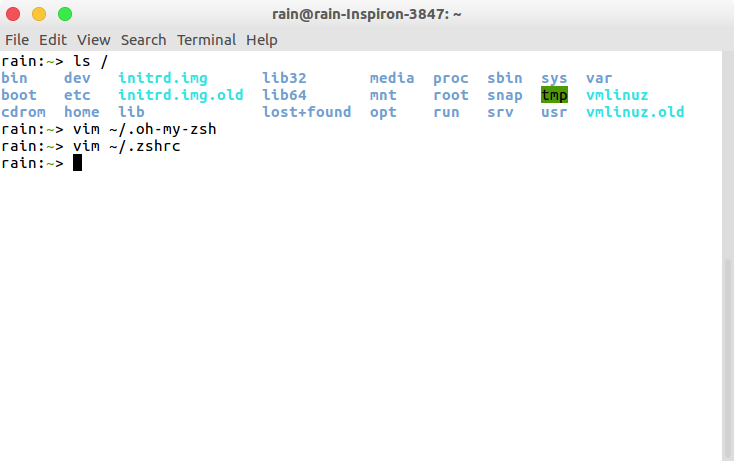
\includegraphics[width=10cm]{images/computer_science/ubuntu/terminal.png}

\textbf{Chuyện bộ gõ}

Làm sao để khởi động lại ibus, thỉnh thoảng lại chết bất đắc kì tử

\begin{lstlisting}
ibus-daemon &
ibus restart
\end{lstlisting}

\textbf{Chuyện lỗi login loop}

Phiên bản: `ubuntu 16.04`



\href{https://askubuntu.com/questions/389903/ibus-doesnt-seem-to-restart}{https://askubuntu.com/questions/389903/ibus-doesnt-seem-to-restart}

\textbf{Hot Corner và Workspace}

Cần cài đặt ngay \textbf{gnome-tweak-tool}

\begin{lstlisting}
sudo apt install gnome-tweak-tool
\end{lstlisting}

Cài đặt hot corner với

\href{https://askubuntu.com/questions/975348/how-to-get-all-hot-corner-in-ubuntu-17-10}{https://askubuntu.com/questions/975348/how-to-get-all-hot-corner-in-ubuntu-17-10}

Cài đặt Workspace
  \part{Khoa học dữ liệu}

%\chapter{Data Science with Python}

View online \href{http://magizbox.com/training/ml_data_python/site/}{http://magizbox.com/training/ml_data_python/site/}

The ability to analyze data with Python is critical in data science. Learn the basics, and move on to create stunning visualizations.

\section{Get Started}

Get Started with Ubuntu
Requirements

numpy, scipy
matplotlib
pandas
scikit-learn
ipython
Install pip

sudo apt-get install python-pip
Install numpy scipy

sudo apt-get install python-numpy python-scipy \
    python-matplotlib python-pandas python-sympy python-nose
Install scikit-learn

pip install jupyter ipython pip install -U scikit-learn

\section{Data Transformation}

DataFrame is a 2-dimensional labeled data structure with columns of potentially different types. You can think of it like a spreadsheet or SQL table, or a dict of Series objects. It is generally the most commonly used pandas object

Create data frame
Create new data frame from lists

\begin{lstlisting}[language=Python]
import pandas as pd
students = pd.DataFrame({
  "name" : ["Kate", "John", "Tom", "Mark"],
  "age" : [20, 21, 19, 18]
})
#       age  name
#    0   20  Kate
#    1   21  John
#    2   19   Tom
#    3   18  Mark
\end{lstlisting}

Load dataframe
Load dataframe from datasets


\begin{lstlisting}[language=Python]
import pandas as pd
from sklearn import datasets
iris_data = datasets.load_iris()
iris = pd.DataFrame(data=iris_data.data,
                    columns=iris_data.feature_names)
iris

\end{lstlisting}

Selection

Select by column index

\begin{lstlisting}[language=Python]
students.iloc[1:3, :]
#       age  name
#    1   21  John
#    2   19   Tom
\end{lstlisting}

Filter

\begin{lstlisting}[language=Python]
students = pd.DataFrame({
  'math' : [90, 80, 95, 50],
  'physic' : [20, 50, 95, 60]
})
#    math  physic
# 0    90      20
# 1    80      50
# 2    95      95
# 3    50      60

students[students['math'] > 85]
#    math  physic
# 0    90      20
# 2    95      95

students[students['math'] == students['physic']]
#    math  physic
# 2    95      95
\end{lstlisting}

Create new column

\begin{lstlisting}[language=Python]
students = pd.DataFrame({
  'name' : ["Kate", "John", "Tom", "Mark"],
  'age' : [20, 21, 19, 18]
})
students["birthyear"] = students.apply(
  lambda row: 2016 - row['age'], axis=1)
students["birthyear"] = 2016 - students["age"]
#       age  name  birthyear
#    0   20  Kate       1996
#    1   21  John       1995
#    2   19   Tom       1997
#    3   18  Mark       1998
\end{lstlisting}

Delete column

\begin{lstlisting}[language=Python]
students = pd.DataFrame({
  'name' : ["Kate", "John", "Tom", "Mark"],
  'age' : [20, 21, 19, 18]
})
students = students.drop('age', 1)
\end{lstlisting}

References

Wes McKinney, 10-minute tour of pandas: video, notebook

DataFrame, Intro to Data Structures

\section{Data Preperation}

Normalization

Example

\begin{lstlisting}[language=Python]
import numpy
from sklearn.preprocessing import normalize
matrix = numpy.arange(0,27,3).reshape(3,3).astype(numpy.float64)

# array([[  0.,   3.,   6.],
#   [  9.,  12.,  15.],
#   [ 18.,  21.,  24.]])

normed_matrix = normalize(matrix, axis=1, norm=‘l1’)

# [[ 0.          0.33333333  0.66666667]
# [ 0.25        0.33333333  0.41666667]
# [ 0.28571429  0.33333333  0.38095238]]
\end{lstlisting}

Label Encoder

Encode labels (categorical variables) with value between 0 and n_classes-1.

\begin{lstlisting}[language=Python]
import sklearn
le = sklearn.preprocessing.LabelEncoder()
le.fit([“paris”, “paris”, “tokyo”, “amsterdam”])
# LabelEncoder()
list(le.classes_)
# [‘amsterdam’, ‘paris’, ‘tokyo’]
le.transform([“tokyo”, “tokyo”, “paris”])
# array([2, 2, 1]...)
list(le.inverse_transform([2, 2, 1]))
# [‘tokyo’, ‘tokyo’, ‘paris’]
\end{lstlisting}

References

How to normalize a 2-dimensional numpy array in python less verbose?
sklearn.preprocessing.LabelEncoder

\section{Data IO}

This post shows how to import data to Python from numerous resources

CSV

Read a csv file from local or from a server

\begin{lstlisting}[language=Python]
import numpy as np
import pandas as pd
# read data
df = pd.read_csv(“data.csv”, header = 0)
# write data
df.to_csv(“data.csv”, header=1, index=False)
\end{lstlisting}

Excel

\begin{lstlisting}[language=Python]
import pandas as pd
# read data
df = pd.read_excel(“data.xls”)
# write data
df = pd.to_excel(“data.xls”, index=False)
\end{lstlisting}

Sqlite

\begin{lstlisting}[language=Python]
import sqlite3

DB_NAME = “db.sqlite3”
SELECT_QUERY = “SELECT page_id, type FROM service_page”
# connect to sqlite3
db_connector = sqlite3.connect(DB_NAME)
# excute query
cursor = db_connector.execute(SELECT_QUERY)
# return dataset
data_set = cursor.fetchall()
\end{lstlisting}

References

pandas.read_excel
pandas.read_sqlite
sqlite3.read_sqlite

\section{Numpy}

NumPy

Use the following import convention:

\begin{lstlisting}[language=Python]
import numpy as np
\end{lstlisting}

Creating Arrays

\begin{lstlisting}[language=Python]
a = np.array([1, 2, 3])
b = np.array([(1.5, 2, 3), (4, 5, 6)], dtype=float)
c = np.array([[(1.5, 2, 3), (4, 5, 6)], [(3, 2, 1), (4, 5, 6)]], dtype=float)
\end{lstlisting}

Initial Placeholders

\begin{lstlisting}[language=Python]
# Create an array of zeros
np.zeros((3, 4))
array([[ 0., 0., 0., 0.], [ 0., 0., 0., 0.], [ 0., 0., 0., 0.]])
\end{lstlisting}

# Create an array of ones

\begin{lstlisting}[language=Python]
np.ones((2, 3, 4), dtype=np.int16)

    array([[[1, 1, 1, 1],
            [1, 1, 1, 1],
            [1, 1, 1, 1]],

           [[1, 1, 1, 1],
            [1, 1, 1, 1],
            [1, 1, 1, 1]]], dtype=int16)

# Create an array of evenly spaced values (step value)
np.arange(10, 25, 5)
array([10, 15, 20])
# Create an array of evenly spaced values (number of samples)
np.linspace(0, 2, 9)
array([ 0. , 0.25, 0.5 , 0.75, 1. , 1.25, 1.5 , 1.75, 2. ])
# Create a constant array
np.full((2, 2), 7)
# array([[ 7., 7.], [ 7., 7.]])

# Create a 2x2 identity matirx
np.eye(2)
array([[ 1., 0.], [ 0., 1.]])
# Create an array with random values
np.random.random((2, 2))
array([[ 0.11121701, 0.12191919], [ 0.61608418, 0.91899253]])
# Create an empty array
np.empty((3, 2))
array([[ 0., 0.], [ 0., 0.], [ 0., 0.]])
\end{lstlisting}

IO

Saving & Loading On Disk

\begin{lstlisting}[language=Python]
a = np.array([(1, 2), (3, 4)])
b = np.array([(5, 6), (7, 8)])
np.save(‘my_array’, a)
np.savez(‘arrays’, a, b)
np.load(‘arrays.npz’)
\end{lstlisting}

Saving & Loading Text Files

\begin{lstlisting}[language=Python]
np.loadtxt(“myfile.txt”)
array([[ 1., 2., 3.], [ 2., 3., 4.]])
np.genfromtxt(“my_file.csv”, delimiter=”,“)
array([[ 1., 2., 3.], [ 4., 5., 6.]])
a = np.array([(1.5, 2, 3), (4, 5, 6)], dtype=float)
np.savetxt(“myarray.txt”, a, delimiter=” “)
\end{lstlisting}

Data Types

\begin{lstlisting}[language=Python]
# Signed 64-bit integer types
np.int64
# Stardard double-precision floating point
np.float32
# Complex numbers represented by 128 floats
np.complex
# Boolean type storing TRUE and FALSE values
np.bool
# Python object type
np.object
# Fixed-length string type
np.string_
# Fixed-length unicode type
np.unicode_
numpy.unicode_
\end{lstlisting}

Inspecting Your Array

\begin{lstlisting}[language=Python]
a = np.array([(1.5, 2, 3), (4, 5, 6)], dtype=float)
# array dimensions
a.shape
(2L, 3L)
# length of array
len(a)
2
# number of array dimensions
a.ndim
2
# number of array elements
a.size
6
# data type of array elements
a.dtype
dtype(‘float64’)
# name of data type
a.dtype.name
‘float64’
# convert an array to a different type
a.astype(int)
array([[1, 2, 3], [4, 5, 6]])
\end{lstlisting}

Asking For Help

\begin{lstlisting}[language=Python]
np.info(np.ndarray.dtype)
\end{lstlisting}

Data-type of the array’s elements. Parameters ————— None Returns ———- d : numpy dtype object See Also ———— numpy.dtype Examples ———— >>> x array([[0, 1], [2, 3]]) >>> x.dtype dtype(‘int32’) >>> type(x.dtype)

Array Mathmatics

Arithmetic Operations

\begin{lstlisting}[language=Python]
a = np.random.random((2, 2))
b = np.random.random((2, 2))
# subtraction
np.subtract(a, b)
a - b
array([[-0.04906355, 0.24579184], [ 0.45085259, 0.55266361]])
# addition
np.add(b, a)
b + a
array([[ 0.11861634, 1.28886181], [ 0.84371684, 1.37134298]])
# division
np.divide(a, b)
a / b
array([[ 0.41479504, 1.47128543], [ 3.29520803, 2.35013443]])
# multiplication
np.multiply(a, b)
a * b
array([[ 0.00291565, 0.40018778], [ 0.12714751, 0.39378613]])
# exponentiation
np.exp(b)
array([[ 1.08745483, 1.68461152], [ 1.21705271, 1.50582314]])
# square root
np.exp(b)
array([[ 1.08745483, 1.68461152], [ 1.21705271, 1.50582314]])
# sines of an array
np.sin(a)
array([[ 0.03476938, 0.69421365], [ 0.60302258, 0.82033885]])
# cosine of an array
np.cos(b)
array([[ 0.99648749, 0.86705545], [ 0.98076917, 0.91738383]])
# natural algorithm
np.log(a)
array([[-3.35881648, -0.26484246], [-0.43496903, -0.03873741]])
# dot product
a.dot(b)
np.dot(a, b)
array([[ 0.15364329, 0.33223443], [ 0.24323666, 0.73136775]])
\end{lstlisting}

Comparison

\begin{lstlisting}[language=Python]
a = np.random.random((2, 2))
a
array([[ 0.20271908, 0.83347777], [ 0.61463859, 0.47298106]])
b = np.random.random((2, 2))
b
array([[ 0.71492635, 0.48317927], [ 0.83547998, 0.67228618]])
# element-wise comparison
a == b
array([[False, False], [False, False]], dtype=bool)
# element-wise comparison
a < 2
array([[ True, True], [ True, True]], dtype=bool)
# array-wise comparison
np.array_equal(a, b)
False
\end{lstlisting}

Aggregate Functions

\begin{lstlisting}[language=Python]
a = np.random.random((3, 3))
a
array([[ 0.71770831, 0.895387 , 0.58199526], [ 0.32399079, 0.24146174, 0.59422847], [ 0.9976845 , 0.36588863, 0.67375734]])
# array-wise sum
a.sum()
5.392102026407013
# array-wise minimum value
a.min()
0.2414617386336485
# maximum value of an array row
a.max(axis=0)
array([ 0.9976845 , 0.895387 , 0.67375734])
# cumulative sum of the elements
a.cumsum(axis=1)
array([[ 0.71770831, 1.61309531, 2.19509057], [ 0.32399079, 0.56545253, 1.15968099], [ 0.9976845 , 1.36357313, 2.03733047]])
# mean
a.mean()
0.59912244737855702
# median
np.median(a)
0.59422846515666305
# correlation coefficient
np.corrcoef(a)
array([[ 1. , -0.93042812, -0.55310242], [-0.93042812, 1. , 0.20930732], [-0.55310242, 0.20930732, 1. ]])
# stardard deviation
np.std(a)
0.24142891382802531
Copy Arrays
a = np.random.random((3, 3))
a
array([[ 0.25274882, 0.19042929, 0.16823795], [ 0.39392342, 0.05954749, 0.8608243 ], [ 0.99375507, 0.92845989, 0.45681322]])
a.view()
array([[ 0.25274882, 0.19042929, 0.16823795], [ 0.39392342, 0.05954749, 0.8608243 ], [ 0.99375507, 0.92845989, 0.45681322]])
np.copy(a)
array([[ 0.25274882, 0.19042929, 0.16823795], [ 0.39392342, 0.05954749, 0.8608243 ], [ 0.99375507, 0.92845989, 0.45681322]])
h = a.copy()
h
array([[ 0.25274882, 0.19042929, 0.16823795], [ 0.39392342, 0.05954749, 0.8608243 ], [ 0.99375507, 0.92845989, 0.45681322]])
\end{lstlisting}

Sorting Arrays

\begin{lstlisting}[language=Python]
a = np.random.random((3, 3))
a
array([[ 0.11422752, 0.30046885, 0.15876115], [ 0.89595996, 0.47878824, 0.41827471], [ 0.69593773, 0.52119338, 0.33048738]])
a.sort()
a
array([[ 0.11422752, 0.15876115, 0.30046885], [ 0.41827471, 0.47878824, 0.89595996], [ 0.33048738, 0.52119338, 0.69593773]])
a.sort(axis=0)
a
array([[ 0.11422752, 0.15876115, 0.30046885], [ 0.33048738, 0.47878824, 0.69593773], [ 0.41827471, 0.52119338, 0.89595996]])
\end{lstlisting}

Subsetting, Slicing, Indexing

Subsettings

\begin{lstlisting}[language=Python]
a = np.random.random((3, 3))
a
array([[ 0.07989823, 0.4180309 , 0.83932547], [ 0.06318651, 0.20509151, 0.08262809], [ 0.64938826, 0.531026 , 0.38633983]])
# select the element at the 2nd index
a[2]
array([ 0.64938826, 0.531026 , 0.38633983])
# select the element at row 0 column 2
a[1][2]
a[1, 2]
0.08262808937797228
\end{lstlisting}

Slicing

\begin{lstlisting}[language=Python]
# select items at index 0 and 1
a[0:2]
array([[ 0.07989823, 0.4180309 , 0.83932547], [ 0.06318651, 0.20509151, 0.08262809]])
# select items at rớ 0 and 1 in column 1
a[0:2, 1]
array([ 0.4180309 , 0.20509151])
# select all items at row 0
a[1, ...]
a[1, ]
array([ 0.06318651, 0.20509151, 0.08262809])
# reversed array a
a[::-1]
array([[ 0.64938826, 0.531026 , 0.38633983], [ 0.06318651, 0.20509151, 0.08262809], [ 0.07989823, 0.4180309 , 0.83932547]])
\end{lstlisting}

Boolean indexing

\begin{lstlisting}[language=Python]
# select elements from a less than 0.5
a[a < 0.5]
array([ 0.07989823, 0.4180309 , 0.06318651, 0.20509151, 0.08262809, 0.38633983])
\end{lstlisting}

Fancy indexing

\begin{lstlisting}[language=Python]
# select elements (1,0), (0,1), (1, 2) and (0,0)
a[[1, 0, 1, 0], [0, 1, 2, 0]]
array([ 0.06318651, 0.4180309 , 0.08262809, 0.07989823])
# select a subset of the matrix’s rows and columns
a[[1, 0, 1, 0]][:, [0, 1, 2, 0]]
array([[ 0.06318651, 0.20509151, 0.08262809, 0.06318651], [ 0.07989823, 0.4180309 , 0.83932547, 0.07989823], [ 0.06318651, 0.20509151, 0.08262809, 0.06318651], [ 0.07989823, 0.4180309 , 0.83932547, 0.07989823]])
\end{lstlisting}

Array Manipulation

Transposing Array

\begin{lstlisting}[language=Python]
a = np.random.random((2, 3))
a
array([[ 0.57430709, 0.64401188, 0.12761183], [ 0.0726823 , 0.7951682 , 0.54114093]])
# permulate array dimensions
i = np.transpose(a)
i
array([[ 0.57430709, 0.0726823 ], [ 0.64401188, 0.7951682 ], [ 0.12761183, 0.54114093]])
# permulate array dimensions
i.T
array([[ 0.57430709, 0.64401188, 0.12761183], [ 0.0726823 , 0.7951682 , 0.54114093]])
\end{lstlisting}

Changing Array Shape

\begin{lstlisting}[language=Python]
# flatten the array
a.ravel()
array([ 0.57430709, 0.64401188, 0.12761183, 0.0726823 , 0.7951682 , 0.54114093])
# reshape, but don’t change data
a.reshape(3, -2)
array([[ 0.57430709, 0.64401188], [ 0.12761183, 0.0726823 ], [ 0.7951682 , 0.54114093]])
\end{lstlisting}

Adding/Removing Elements

\begin{lstlisting}[language=Python]
# return a new array with shape (2, 6)
a.resize(2, 3)
a
array([[ 0.57430709, 0.64401188, 0.12761183], [ 0.0726823 , 0.7951682 , 0.54114093]])
# append items to an array
h = np.random.random((2, 3))
print “h:”, h
g = np.random.random((2, 3))
print “g:”, g
np.append(h, g)
h: [[ 0.67964404 0.09256795 0.90630423] [ 0.52906489 0.51567697 0.95132012]] g: [[ 0.03126344 0.84908154 0.74228134] [ 0.40333143 0.28595213 0.68416838]] array([ 0.67964404, 0.09256795, 0.90630423, 0.52906489, 0.51567697, 0.95132012, 0.03126344, 0.84908154, 0.74228134, 0.40333143, 0.28595213, 0.68416838])
# insert items in an array
a = np.random.random((1, 3))
print “a:”, a
np.insert(a, 1, 0.5)
a: [[ 0.76135438 0.30331334 0.91866363]] array([ 0.76135438, 0.5 , 0.30331334, 0.91866363])
# delete items from an array
a = np.random.random((1, 3))
print “a:”, a
np.delete(a, [1])
a: [[ 0.1034073 0.93066432 0.49608264]] array([ 0.1034073 , 0.49608264])
\end{lstlisting}

Combining Arrays

\begin{lstlisting}[language=Python]
# concatenate arrays
a = np.random.random((1, 3))
print a
b = np.random.random((1, 3))
print b
np.concatenate((a, b), axis=0)
[[ 0.34496986 0.59502574 0.43416152]] [[ 0.98921435 0.68832237 0.44286195]] array([[ 0.34496986, 0.59502574, 0.43416152], [ 0.98921435, 0.68832237, 0.44286195]])
# stack arrays vertically (row-wise)
a = np.random.random((1, 3))
print a
b = np.random.random((2, 3))
print b
np.vstack((a, b)) #  equivalent to np.r_[a, b]
[[ 0.78793841 0.9923401 0.96372077]] [[ 0.75537083 0.09781391 0.25327948] [ 0.20607759 0.03763863 0.30818643]] array([[ 0.78793841, 0.9923401 , 0.96372077], [ 0.75537083, 0.09781391, 0.25327948], [ 0.20607759, 0.03763863, 0.30818643]])
# stack arrays horizontally (column-wise)
a = np.random.random((3, 1))
print a
b = np.random.random((3, 2))
print b
np.hstack((a, b))
[[ 0.33728008] [ 0.1091688 ] [ 0.68714517]] [[ 0.61421635 0.49316384] [ 0.19072731 0.04383904] [ 0.30587218 0.28743208]] array([[ 0.33728008, 0.61421635, 0.49316384], [ 0.1091688 , 0.19072731, 0.04383904], [ 0.68714517, 0.30587218, 0.28743208]])
# equivalent to np.hstack
np.column_stack((a, b))
array([[ 0.33728008, 0.61421635, 0.49316384], [ 0.1091688 , 0.19072731, 0.04383904], [ 0.68714517, 0.30587218, 0.28743208]])
# equivalent to np.hstack
np.c_[a, b]
array([[ 0.33728008, 0.61421635, 0.49316384], [ 0.1091688 , 0.19072731, 0.04383904], [ 0.68714517, 0.30587218, 0.28743208]])
\end{lstlisting}

Spliting Arrays

\begin{lstlisting}[language=Python]
a = np.random.random((3, 4))
print a
[[ 0.64277816 0.75935599 0.64927247 0.80253242] [ 0.87630664 0.19748931 0.51895547 0.83645583] [ 0.03132085 0.043291 0.10945252 0.31883126]]
# split the array horizontally at the 3rd index
np.split(a, 3)
[array([[ 0.64277816, 0.75935599, 0.64927247, 0.80253242]]), array([[ 0.87630664, 0.19748931, 0.51895547, 0.83645583]]), array([[ 0.03132085, 0.043291 , 0.10945252, 0.31883126]])]
# split the array vertically at the 3rd index
np.vsplit(a, 3)
[array([[ 0.64277816, 0.75935599, 0.64927247, 0.80253242]]), array([[ 0.87630664, 0.19748931, 0.51895547, 0.83645583]]), array([[ 0.03132085, 0.043291 , 0.10945252, 0.31883126]])]
\end{lstlisting}

Suggested Readings
www.datacamp.com. Python For Data Science Cheat Sheet: Numpy Basics

\section{Data Wrangling}

Learn about data wrangling with pandas

Tiny Data
A foundation for wrangling in pandas

Create DataFrames
Specify values for each column

\begin{lstlisting}[language=Python]
import pandas as pd

df = pd.DataFrame({
“a”: [4, 5, 6],
“b”: [7, 8, 9],
“c”: [10, 11, 12]
}, index=[1, 2, 3])
df
a b c

1 4 7 10

2 5 8 11

3 6 9 12
\end{lstlisting}

Specify values for each row

\begin{lstlisting}[language=Python]
df = pd.DataFrame(
[[4, 5, 6],
[7, 8, 9],
[10, 11, 12]],
index=[1, 2, 3],
columns=[“a”, “b”, “c”])
df
a b c
1 4 5 6
2 7 8 9
3 10 11 12
\end{lstlisting}

Create DataFrame with a MultiIndex

df = pd.DataFrame({
“a”: [4, 5, 6],
“b”: [7, 8, 9],
“c”: [10, 11, 12]
})
index = pd.MultiIndex.from_tuples(
[(‘d’, 1), (‘d’, 2), (‘e’, 2)],
names=[‘n’,‘v’])
df
a b c

0 4 7 10

1 5 8 11

2 6 9 12

Reshaping Data
melt
“Unpivots” a DataFrame from wide format to long format, optionally leaving identifier variables set.

import pandas as pd

df = pd.DataFrame({
“a”: [4, 5],
“b”: [7, 8],
“c”: [10, 11]
})
df
a b c

0 4 7 10

1 5 8 11

pd.melt(df)
variable value

0 a 4

1 a 5

2 b 7

3 b 8

4 c 10

5 c 11

pivot
Reshape data (produce a “pivot” table) based on column values. Uses unique values from index / columns to form axes of the resulting DataFrame.

df = pd.DataFrame({‘foo’: [‘one’,‘one’,‘one’,‘two’,‘two’,‘two’],
‘bar’: [‘A’, ‘B’, ‘C’, ‘A’, ‘B’, ‘C’],
‘baz’: [1, 2, 3, 4, 5, 6]})
df
bar baz foo

0 A 1 one

1 B 2 one

2 C 3 one

3 A 4 two

4 B 5 two

5 C 6 two

df.pivot(index=‘foo’, columns=‘bar’, values=‘baz’)
bar A B C

foo

one 1 2 3

two 4 5 6

df.pivot(index=‘foo’, columns=‘bar’)[‘baz’]
bar A B C

foo

one 1 2 3

two 4 5 6

concat
Append rows of DataFrames

df1 = pd.DataFrame([[‘a’, 1], [‘b’, 2]],
columns=[‘letter’, ‘number’])
df1
letter number

0 a 1

1 b 2

df2 = pd.DataFrame([[‘c’, 3], [‘d’, 4]],
columns=[‘letter’, ‘number’])
pd.concat([df1, df2])
letter number

0 a 1

1 b 2

0 c 3

1 d 4

Append columns of DataFrames

df1 = pd.DataFrame([[‘a’, 1], [‘b’, 2]],
columns=[‘letter’, ‘number’])
df1
letter number

0 a 1

1 b 2

df2 = pd.DataFrame([[‘bird’, ‘polly’], [‘monkey’, ‘george’]],
columns=[‘animal’, ‘name’])
df2
animal name

0 bird polly

1 monkey george

pd.concat([df1, df2], axis=1)
letter number animal name

0 a 1 bird polly

1 b 2 monkey george

sort
df = pd.DataFrame([[‘a’, 10, 1], [‘b’, 10, 5], [‘c’, 30, 3]],
columns=[‘name’, ‘age’, ‘score’])
df
name age score

0 a 10 1

1 b 10 5

2 c 30 3

order rows by values of a column (low to high)

df.sort_values(‘age’)
name age score

0 a 10 1

1 b 10 5

2 c 30 3

order rows by values of a column (high to low)

df.sort_values(‘age’, ascending=False)
name age score

2 c 30 3

0 a 10 1

1 b 10 5

order rows by values of two column

df.sort_values([‘age’, ‘score’], ascending=[False, False])
name age score

2 c 30 3

1 b 10 5

0 a 10 1

sort the index of a DataFrame

df.sort_index()
name age score

0 a 10 1

1 b 10 5

2 c 30 3

Reset index of DataFrame to row numbers, moving index to columns

df.reset_index()
index name age score

0 0 a 10 1

1 1 b 10 5

2 2 c 30 3

drop
drop columns from DataFrame

df.drop([‘age’, ‘score’], axis=1)
name
0	a
1	b
2	c

\section{Visualization}

An introduction about data visualization techniques using Matplotlib and Seaborn.

Gallery
 line graph
Line Graph

 bar graph
Bar Graph

 pie graph
Pie Graph

 sratter plot
Scatter Plot

References
Patterns: The Data Visualisation Catalogue




%\chapter{Trí tuệ nhân tạo}

View online \href{http://magizbox.com/training/ai/site/}{http://magizbox.com/training/ai/site/}

Artificial intelligence (AI) is the intelligence exhibited by machines or software. It is also the name of the academic field of study which studies how to create computers and computer software that are capable of intelligent behavior. Major AI researchers and textbooks define this field as "the study and design of intelligent agents", in which an intelligent agent is a system that perceives its environment and takes actions that maximize its chances of success. John McCarthy, who coined the term in 1955, defines it as "the science and engineering of making intelligent machines".

\section{Autonomous Agents}

limited ability to perceive its environment
process the environment and calculate an action
no global plan / leader
Vehicles

Action / Selection
Steering
Locomotion
Steering Behavior 1 2


Steering = Desired - Velocity

Seek
Flow Filed Following
Path Following
Group Steering
https://github.com/shiffman/The-Nature-of-Code-Examples/tree/master/chp06_agents\

Massive Battle: Coordinated Movement of Autonomous Agents ↩

Craig Reynolds, Steering Behaviors For Autonomous Characters ↩

\section{Cellular Automator}

https://www.youtube.com/watch?v=DKGodqDs9sA&index=1&list=PLRqwX-V7Uu6YrWXvEQFOGbCt6cX83Xunm

Cellular Automata

Grid of cell
Each cell has state, neighborhood
cell state at time t defined by a function of neighborhood states at time t-1
Elementary Cellular Automata

\section{Fractal}

L-System

\section{The Pac-Man project}

Today I found an interesting AI project - The Pac-Man

http://ai.berkeley.edu/images/pacman_game.gif

Here is the project overview

The Pac-Man projects were developed for UC Berkeley's introductory artificial intelligence course, CS 188. They apply an array of AI techniques to playing Pac-Man. However, these projects don't focus on building AI for video games. Instead, they teach foundational AI concepts, such as informed state-space search, probabilistic inference, and reinforcement learning. These concepts underly real-world application areas such as natural language processing, computer vision, and robotics. We designed these projects with three goals in mind. The projects allow students to visualize the results of the techniques they implement. They also contain code examples and clear directions, but do not force students to wade through undue amounts of scaffolding. Finally, Pac-Man provides a challenging problem environment that demands creative solutions; real-world AI problems are challenging, and Pac-Man is too. In our course, these projects have boosted enrollment, teaching reviews, and student engagement. The projects have been field-tested, refined, and debugged over multiple semesters at Berkeley. We are now happy to release them to other universities for educational use.
In the next part of this post, I will show my works on this project

Project 1: Search in Pacman

[caption id="" align="alignleft" width="231"]DFS[/caption]

[caption id="" align="alignleft" width="233"]BFS[/caption]
%\chapter{Học máy}

View online \href{http://magizbox.com/training/machinelearning/site/}{http://magizbox.com/training/machinelearning/site/}

\begin{itemize}
  \item Vấn đề với HMM và CRF?
  \item Học MLE và MAP?
\end{itemize}



Machine learning is a branch of science that deals with programming the systems in such a way that they automatically learn and improve with experience. Here, learning means recognizing and understanding the input data and making wise decisions based on the supplied data.

We can think of machine learning as approach to automate tasks like predictions or modelling. For example, consider an email spam filter system, instead of having programmers manually looking at the emails and coming up with spam rules. We can use a machine learning algorithm and feed it input data (emails) and it will automatically discover rules that are powerful enough to distinguish spam emails.

Machine learning is used in many application nowadays like spam detection in emails or movie recommendation systems that tells you movies that you might like based on your viewing history. The nice and powerful thing about machine learning is: It learns when it gets more data and hence it gets more and more powerful the more data we give them.

**Có bao nhiêu thuật toán Machine Learning?**

Có rất nhiều thuật toán Machine Learning, bài viết [Điểm qua các thuật toán Machine Learning hiện đại](https://ongxuanhong.wordpress.com/2015/10/22/diem-qua-cac-thuat-toan-machine-learning-hien-dai/) của Ông Xuân Hồng tổng hợp khá nhiều thuật toán. Theo đó, các thuật toán Machine Learning được chia thành các nhánh lớn như `regression`, `bayesian`, `regularization`, `decision tree`, `instance based`, `dimesionality reduction`, `clustering`, `deep learning`, `neural networks`, `associated rule`, `ensemble`... Ngoài ra thì còn có các cheatsheet của [sklearn](http://scikit-learn.org/stable/tutorial/machine_learning_map/index.html).

Việc biết nhiều thuật toán cũng giống như ra đường mà có nhiều lựa chọn về xe cộ. Tuy nhiên, quan trọng là có task để làm, sau đó thì cập nhật SOTA của task đó để biết các công cụ mới.

**Xây dựng model cần chú ý điều gì?**

Khi xây dựng một model cần chú ý đến vấn đề tối ưu hóa tham số (có thể sử dụng [GridSearchCV](sklearn.model_selection.GridSearchCV))

Bài phát biểu này có vẻ cũng rất hữu ích [PYCON UK 2017: Machine learning libraries you'd wish you'd known about](https://www.youtube.com/watch?v=nDF7_8FOhpI). Có đề cập đến

* [DistrictDataLabs/yellowbrick](https://github.com/DistrictDataLabs/yellowbrick) (giúp visualize model được train bởi sklearn)
* [marcotcr/lime](https://github.com/marcotcr/lime) (giúp inspect classifier)
* [TeamHG-Memex/eli5](https://github.com/TeamHG-Memex/eli5) (cũng giúp inspect classifier, hỗ trợ nhiều model như xgboost, crfsuite, đặc biệt có TextExplainer sử dụng thuật toán từ eli5)
* [rhiever/tpot](https://github.com/rhiever/tpot) (giúp tối ưu hóa pipeline)
* [dask/dask](https://github.com/dask/dask) (tính toán song song và lập lịch)

Ghi chú về các thuật toán trong xử lý ngôn ngữ tự nhiên tại [underthesea.flow/wiki](https://github.com/magizbox/underthesea.flow/wiki/Develop)

Framework để train, test hiện tại vẫn rất thoải mái sklearn. tensorboard cung cấp phần log cũng khá hay.

[Câu trả lời hay](https://www.quora.com/What-are-the-most-important-machine-learning-techniques-to-master-at-this-time/answer/Sean-McClure-3?srid=5O2u) cho câu hỏi [Những kỹ thuật machine learning nào quan trọng nhất để master?](https://www.quora.com/What-are-the-most-important-machine-learning-techniques-to-master-at-this-time), đặc biệt là dẫn đến bài [The State of ML and Data Science 2017](https://www.kaggle.com/surveys/2017) của Kaggle.

**Tài liệu học PGM**

[Playlist youtube](https://www.youtube.com/watch?v=WPSQfOkb1M8&amp;list=PL50E6E80E8525B59C) khóa học Probabilistic Graphical Models của cô Daphne Koller. Ngoài ra còn có một [tutorial](http://mensxmachina.org/files/software/demos/bayesnetdemo.html) dở hơi ở đâu về tạo Bayesian network

**[Chưa biết] Tại sao Logistic Regression lại là Linear Model?**

Trong quyển Deep Learning, chương 6, trang 165, tác giả có viết

```
Linear models, such as logistic regression and linear
regression, are appealing because they can be fit
efficiently and reliably, either in closed form or
with convex optimization
```

Mình tự hỏi tại sao logistic regression lại là linear, trong khi nó có sử dụng hàm logit (nonlinear)? Tìm hiểu hóa ra cũng có bạn hỏi giống mình trên [stats.stackexchange.com](https://stats.stackexchange.com/questions/93569/why-is-logistic-regression-a-linear-classifier). Ngoài câu trả lời trên stats.stackexchange, đọc một số cái khác [Generalized Linear Models, SPSS Statistics 22.0.0](https://www.ibm.com/support/knowledgecenter/en/SSLVMB_22.0.0/com.ibm.spss.statistics.help/spss/advanced/idh_idd_genlin_typeofmodel.htm)
và [6.1 - Introduction to Generalized Linear Models, Analysis of Discrete Data, Pennsylvania State University](https://onlinecourses.science.psu.edu/stat504/node/216) cũng vẫn chưa hiểu lắm.

Hiện tại chỉ hiểu là các lớp model này chỉ có thể hoạt động trên các tập linear separable, có lẽ do việc map input x, luôn có một liên kết linear $latex wx$, trước khi đưa vào hàm non-linear.

**Các tập dữ liệu thú vị**

*Iris dataset*: dữ liệu về hoa iris

Là một ví dụ cho bài toán phân loại

*Weather problem*: dữ liệu thời tiết. Có thể tìm được ở trong quyển Data Mining: Practical Machine Learning Tools and Techniques

Là một ví dụ cho bài toán cây quyết định

## Deep Learning

**Tài liệu Deep Learning**

Lang thang thế nào lại thấy trang này [My Reading List for Deep Learning!](https://www.microsoft.com/en-us/research/wp-content/uploads/2017/02/DL_Reading_List.pdf) của một anh ở Microsoft. Trong đó, (đương nhiên) có Deep Learning của thánh Yoshua Bengio, có một vụ hay nữa là bài review "Deep Learning" của mấy thánh Yann Lecun, Yoshua Bengio, Geoffrey Hinton trên tạp chí Nature. Ngoài ra còn có nhiều tài liệu hữu ích khác.

### Các layer trong deep learning [^2]

#### Sparse Layers

[**nn.Embedding**](http://pytorch.org/docs/master/nn.html#embedding) ([hướng dẫn](http://pytorch.org/tutorials/beginner/nlp/word_embeddings_tutorial.html))
★ grep code: [Shawn1993/cnn-text-classification-pytorch](https://github.com/Shawn1993/cnn-text-classification-pytorch/blob/master/model.py#L18)
Đóng vai trò như một lookup table, map một word với dense vector tương ứng

#### Convolution Layers

[**nn.Conv1d**](http://pytorch.org/docs/master/nn.html#conv1d), [**nn.Conv2d**](http://pytorch.org/docs/master/nn.html#conv2d), [**nn.Conv3d**](http://pytorch.org/docs/master/nn.html#conv3d) [^1]
★ grep code: [Shawn1993/cnn-text-classification-pytorch](https://github.com/Shawn1993/cnn-text-classification-pytorch/blob/master/model.py#L20-L24), [galsang/CNN-sentence-classification-pytorch](https://github.com/galsang/CNN-sentence-classification-pytorch/blob/master/model.py#L36-L38)

Các tham số trong Convolution Layer

* `kernel_size` (hay là filter size)

Đối với NLP, kernel_size thường bằng region_size * word_dim (đối với conv1d) hay (region_size, word_dim) đối với conv2d

<small>Quá trình tạo feature map đối với region size bằng 2</small>
![](https://media.giphy.com/media/l2QE2y1UQP7vIgiti/giphy.gif)

* `in_channels`, `out_channels` (là số lượng `feature maps`)

Kênh (channels) là các cách nhìn (view) khác nhau đối với dữ liệu. Ví dụ, trong ảnh thường có 3 kênh RGB (red, green, blue), có thể áp dụng convolution giữa các kênh. Với văn bản cũng có thể có các kênh khác nhau, như khi có các kênh sử dụng các word embedding khác nhau (word2vec, GloVe), hoặc cùng một câu nhưng biểu diễn ở các ngôn ngữ khác nhau.

* `stride`

Định nghĩa bước nhảy của filter.

![](http://d3kbpzbmcynnmx.cloudfront.net/wp-content/uploads/2015/11/Screen-Shot-2015-11-05-at-10.18.08-AM-1024x251.png)

Hình minh họa sự khác biệt giữa các feature map đối với stride=1 và stride=2. Feature map đối với stride = 1 có kích thước là 5, feature map đối với stride = 3 có kích thước là 3. Stride càng lớn thì kích thước của feature map càng nhỏ.

Trong bài báo của Kim 2014, `stride = 1` đối với `nn.conv2d` và `stride = word_dim` đối với `nn.conv1d`

Toàn bộ tham số của mạng CNN trong bài báo Kim 2014,

![](http://d3kbpzbmcynnmx.cloudfront.net/wp-content/uploads/2015/11/Screen-Shot-2015-11-06-at-8.03.47-AM.png)

| Description | Values |
|---------------------|-----------------|
| input word vectors | Google word2vec |
| filter region size | (3, 4, 5)       |
| feature maps | 100 |
| activation function | ReLU |
| pooling | 1-max pooling |
| dropout rate | 0.5 |
| $latex l&amp;s=2$2 norm constraint | 3 |

Đọc thêm:

* [Lecture 13: Convolutional Neural Networks (for NLP). CS224n-2017](http://web.stanford.edu/class/cs224n/lectures/cs224n-2017-lecture13-CNNs.pdf)
* [DeepNLP-models-Pytorch - 8. Convolutional Neural Networks](https://nbviewer.jupyter.org/github/DSKSD/DeepNLP-models-Pytorch/blob/master/notebooks/08.CNN-for-Text-Classification.ipynb)
* [A Sensitivity Analysis of (and Practitioners’ Guide to) Convolutional Neural Networks for Sentence Classification. Zhang 2015](https://arxiv.org/pdf/1510.03820.pdf)

**BTS**

22/11/2017 - Phải nói quyển này hơi nặng so với mình. Nhưng thôi cứ cố gắng vậy.
24/11/2017 - Từ hôm nay, mỗi ngày sẽ ghi chú một phần (rất rất nhỏ) về Deep Learning [tại đây](https://docs.google.com/document/d/1KxDrw5s6uYHNLda7t0rhp0RM_TlUGxydQ-Qi1JOPFr8/edit?usp=sharing)

[^1]: [Understanding Convolutional Neural Networks for NLP](http://www.wildml.com/2015/11/understanding-convolutional-neural-networks-for-nlp)
[^2]: [http://pytorch.org/docs/master/nn.html](http://pytorch.org/docs/master/nn.html)

\section{Machine Learning Process}

The good life is a process, not a state of being. It is a direction not a destination.

Carl Rogers


I searched a framework fit for every data mining task, I found a good one from an article of Oracle.

And here is my summary. The data mining process has 4 steps:

Step 1. Problem Definition

This initial phase of a data mining project focuses on understanding the project objectives and requirements. Once you have specified the project from a business perspective, you can formulate it as a data mining problem and develop a preliminary implementation plan.

Step 2. Data Gathering & Preparation

The data understanding phase involves data collection and exploration. As you take a closer look at the data, you can determine how well it addresses the business problem. You might decide to remove some of the data or add additional data. This is also the time to identify data quality problems and to scan for patterns in the data.

Data Access
Data Sampling

Data Transformation

Data in the real world is dirty [3]. They are often incomplete (lacking attribute values, lacking certain attributes of interest, or containing only aggregate data), noisy (containing errors or outliers),‰ inconsistent (containing discrepancies in codes or names). Step 3. Model Building In this phase, you select and apply various modeling techniques and calibrate the parameters to optimal values. If the algorithm requires data transformations, you will need to step back to the previous phase to implement them

Create Model
Test Model

Evaluate & Interpret Model

Some important questions [2]:

Is at least one of predictors useful in predicting the response? (F-statistics)
Do all the predictors help to explain Y, or is only a subset of the predictors useful? (all subsets or best subsets)
How well does the model fit the data?
Given a set of predictor values, what response value should we predict, and how accurate is our prediction?
Step 4. Knowledge Deployment Knowledge deployment is the use of data mining within a target environment. In the deployment phase, insight and actionable information can be derived from data.
Model Apply
Custom Reports
External Applications
References
The Data Mining Process, Oracle
Trevor Hastie and Rob Tibshirani, Model Selection and Qualitative Predictors, URL:https://www.youtube.com/watch?v=3T6RXmIHbJ4
Nguyen Hung Son, Data cleaning and Data preprocessing, URL:http://www.mimuw.edu.pl/~son/datamining/DM/4-preprocess.pdf

\subsection{Problem Definition}

This initial phase of a data mining project focuses on understanding the project objectives and requirements. Once you have specified the project from a business perspective, you can formulate it as a data mining problem and develop a preliminary implementation plan.

For example, your business problem might be: "How can I sell more of my product to customers?" You might translate this into a data mining problem such as: "Which customers are most likely to purchase the product?" A model that predicts who is most likely to purchase the product must be built on data that describes the customers who have purchased the product in the past. Before building the model, you must assemble the data that is likely to contain relationships between customers who have purchased the product and customers who have not purchased the product. Customer attributes might include age, number of children, years of residence, owners/renters, and so on.

\subsection{Data Gathering}

The data understanding phase involves data collection and exploration. As you take a closer look at the data, you can determine how well it addresses the business problem. You might decide to remove some of the data or add additional data. This is also the time to identify data quality problems and to scan for patterns in the data.

The data preparation phase covers all the tasks involved in creating the case table you will use to build the model. Data preparation tasks are likely to be performed multiple times, and not in any prescribed order. Tasks include table, case, and attribute selection as well as data cleansing and transformation. For example, you might transform a DATE_OF_BIRTH column to AGE; you might insert the average income in cases where the INCOME column is null.

Additionally you might add new computed attributes in an effort to tease information closer to the surface of the data. For example, rather than using the purchase amount, you might create a new attribute: "Number of Times Amount Purchase Exceeds $500 in a 12 month time period." Customers who frequently make large purchases may also be related to customers who respond or don't respond to an offer.

Thoughtful data preparation can significantly improve the information that can be discovered through data mining.

Data Sources
Open Data

wikipedia dumps: https://dumps.wikimedia.org/other/pagecounts-raw/

\subsection{Data Preprocessing}

The quality of the data and the amount of useful information it contains affect greatly how well an algorithm can learn. Hence, it is important to preprocess the dataset before using it. The most common preprocessing steps are: removing missing values, converting categorical data into shape suitable for machine learning algorithm and feature scaling.

Missing Data
Sometimes the samples in the dataset are missing some values and we want to deal with these missing values before passing it to the machine learning algorithm. There are a number of strategies we can follow

Remove samples with missing values: This approach is by far the most convenient but we may end up removing too many samples and by that we would be losing valuable information that can help the machine learning algorithm.
Imputing missing values: Instead of removing the entire sample we use interpolation to estimate the missing values. For example, we could substitute a missing value by the mean of the entire column.
Categorical Data
In general, features can be numerical (e.g. price, length, width, etc…) or categorical (e.g. color, size, etc..). Categorical features are further split into nominal and ordinal features.

Ordinal features can be sorted and ordered. For example, size (small, medium, large), we can order these sizes large > medium > small. While nominal features do not have an order for example, color, it doesn’t make any sense to say that red is larger than blue.

Most machine learning algorithm require that you convert categorical features into numerical values. One solution would to assign each value a different number starting from zero. (e.g. small à 0 ,medium à 1 ,large à 2)

This works well for ordinal features but might cause problems with nominal features (e.g. blue à 0, white à 1, yellow à 2) because even though colors are not ordered the learning algorithm will assume that white is larger than blue and yellow is larger than white and this is not correct.

To get around this problem is to use one-hot encoding, the idea is to create a new feature for each unique value of the nominal feature.


In the above example, we converted the color feature into three new features Red, Green, Blue and we used binary values to indicate the color. For example, a sample with “Red” color is now encoded as (Red=1, Green=0, Blue=0)

Feature Scaling
Why have we do Feature Scaling?

We have to predict the house prices base on 2 features:

House sizes (feet2)
Number of bedrooms in the house
And we relized that house sizes are about 1000 times the number of bedrooms. When features differ by orders of magnitude, first performing feature scaling can make gradient descent converge much more quickly.

Perform Feature Scaling

Subtract the mean value (the average value) of each feature from the dataset.
After subtracting the mean, additionally scale (divide) the feature values by their respective "standard deviations."
Function: x′=x−x¯σx′=x−x¯σ where xx is the original feature vector, x¯x¯ is the mean of that feature vector, and σσ is its standard deviation.
Feature Scaling Function implementation in Octave

function [X_norm, mu, sigma] = featureNormalize(X)
X_norm = X;
mu = zeros(1, size(X, 2)); % storing the mean value in mu
sigma = zeros(1, size(X, 2)); % storing the standard deviation in sigma

for i = 1:length(mu),
mu(i) = mean(X(:,i));
end;

for i = 1:length(sigma),
sigma(i) = std(X(:,i));
end;

X_norm = (X .- mu)./sigma;
end
Related Reading
Introduction to Machine Learning

\subsection{Model Building}

In this phase, you select and apply various modeling techniques and calibrate the parameters to optimal values. If the algorithm requires data transformations, you will need to step back to the previous phase to implement them

Create Model
Test Model
Evaluate & Interpret Model
Some important questions

Is at least one of predictors useful in predicting the response? (F-statistics)
Do all the predictors help to explain Y, or is only a subset of the predictors useful? (all subsets or best subsets)
How well does the model fit the data?
Given a set of predictor values, what response value should we predict, and how accurate is our prediction?
Create Model
First thing first, start with simple and fast model, then you known how difficult the problem is.

One import thing is create a well pipeline for your experiments, it is very helpful in turning features, model selection, save your experiment and write reports.

Feature Selections
After train model, some model will give active features (such as CRF), it is clue for you to feature selection. If amount active features is too small compared to amount features, it is the problem. In this case the better way to enhance is try reduce amount of features and see how well this set fit data. Keep in mind the more number of features is, the complex model is, and it will make your model over fitting.
Storing the model
Number of active features: 5566 (35383)
Number of active attributes: 4343 (20722)
example after training crf model with python-crfsuite
Test Model
This phase determines how well the model fit data. See Evaluation for details.

What to do next
In an interview Andrew Ng said about building machine learning model

"I often make an analogy to building a rocket ship. A rocket ship is a giant engine together with a ton of fuel. Both need to be really big. If you have a lot of fuel and a tiny engine, you won’t get off the ground. If you have a huge engine and a tiny amount of fuel, you can lift up, but you probably won’t make it to orbit. So you need a big engine and a lot of fuel.

The reason that machine learning is really taking off now is that we finally have the tools to build the big rocket engine — that is giant computers, that’s our rocket engine. And the fuel is the data. We finally are getting the data that we need."

We need both big rocket engine and data to make our model works.

Related Reading
Inside The Mind That Built Google Brain: On Life, Creativity, And Failure, huffingtonpost.com

\subsection{Evaluation}

Training vs Test Data
We typically split the input data into learning and testing datasets. The then run the machine learning algorithm on the learning dataset to generate the prediction model. Later, we use the test dataset to evaluate our model.


It is important that the test data is separate from the one used in training otherwise we will be kind of cheating because may for example the generated model memorizes the data and hence if the test data is also part of the training data then our evaluation scores of the model will be higher than they actually are.

The data is usually split 75% training and 25% data or 2/3 training and 1/3 testing. It is important to note that: the smaller the training set the more challenging it is for the algorithm to discover the rules.

In addition, when splitting the dataset, you need to maintaining class proportions and population statistics otherwise we will have some classes that are under represented in the training dataset and over represented in the test dataset.

For example, you may have 100 sample and a total of 80 samples are labeled with Class-A and the remaining 20 instances are labeled with Class-B. you want to make sure when splitting the data that you maintain this representation.

One way to avoid this problem and to make sure that all classes are represented in both training and testing datasets is stratification. It is the process of rearranging the data as to ensure each set is a good representative of the whole. In our previous example, (80/20 samples), it is best to arrange the data such that in every set, each class comprises around 80:20 ratios of the two classes.

Cross Validation
A crucial step when building our machine learning model is to estimate its performance on that that the model hadn't seen before. We want to make sure that the model generalizes well to new unseen data.

One case, the machine learning algorithm has different parameters and we want to tune these parameters to achieve the best performance. (Note: the parameters of the machine learning algorithm are called hyperparameters). Another case, sometimes we want to try out different algorithms and choose the best performing one. Below are some of the techniques used.

Holdout Method
We simply split the data into training and testing datasets. We train the algorithm on the training dataset to generate a model. In order, to evaluate different algorithms we use the testing data to evaluate each algorithm.

However, if we reuse the same test dataset over and over again during algorithm selection, the test data has now come part of the training data. Hence, when we use the test data for the final evaluation the generated model is biased towards the test data and the performance score is optimistic.

Holdout Validation
As before, we split the data into training and testing dataset. Then, the training data is further split into training and validation sets.

The training data is used to train different models. Then the validation data is used to compute performance of each of them and we select the best one. Finally, the model is then used for the test set to evaluate performance. The next figure illustrates this idea.


However, because we use the validation set multiple times, Holdout validation is sensitive to how we partition the data and that is what K-fold cross validation tries to solve.

K-fold cross validation
Initially, we split the data into training and testing dataset. Furthermore, the training dataset is split into K chunks.

Suppose we will use 5-fold cross validation, the training data set is split into 5 chunks and the training phase will take place over 5 iterations. In each iteration we use one chunk as the validation dataset while the rest of the chunk are grouped together to form the training dataset.

This is very similar to Holdout validation except in each iteration the validation data is different and this removed the bias. Each iteration generates a score and the final score is the average score of all iteration. As before we select the best model and use the test data for the final performance evaluation.

Related Readings

Introduction to Machine Learning

\section{Types of Machine Learning}

There are three different types of machine learning: supervised, unsupervised and reinforcement learning. 4

Supervised Learning
The goal of supervised learning is to learn a model from labelled training data that allows us to make predictions about future data. For supervised machine learning to work we need to feed the algorithm two things: the input data and our knowledge about it labels).

The spam filter example mentioned earlier is a good example of supervised learning; we have a bunch of emails (data) and we know whether each email is spam or not (labels).


Supervised learning can be divided into two subcategories:

Classification: It is used to predict categories or class labels based on past observations i.e. we have discrete variable you want to distinguish into discrete categorical outcome. For example, in the email spam filter system the output is discrete "spam" or "not spam".
Regression: It is used to predict a continuous outcome. For example, to determine the price of houses and how it is affected by the number of rooms in that house. The input data is the house features (no. of rooms, location, size in square feet,) and the output is the price (the continuous outcome).
Unsupervised Learning
The goal of unsupervised learning is to discover hidden structure or patterns in unlabeled data and it can be divided into two subcategories

Clustering: It is used to organize information into meaningful clusters (subgroups) without having prior knowledge of their meaning. For example, the figure below shows how we can use clustering to organize unlabeled data into groups based on their features.


Dimensionality Reduction (Compression): It is used to reduce a higher dimension data into a lower dimension ones. To put it more clearly consider this example. A telescope has terabytes of data and not all of these data can be stored and so we can use dimensionality reduction to extract the most informative features of these data to be stored. Dimensionality reduction is also a good candidate to visualize data because if you have data in higher dimensions you can compress it to 2D or 3D to easily plot and visualize it.

Reinforcement Learning

The goal of reinforcement learning is to develop a system that improves its performance based on the interaction with a dynamic environment and there is a delayed feedback that act as a reward. i.e. reinforcement learning is learning by doing with a delayed reward. A classic example of reinforcement learning is a chess game, the computer decided a series of moves and the reward is the "win" or "lose" at the end the game.

You might think that this is similar to supervised learning where the reward is basically a label for the data but the core difference is this feedback/reward is not the truth but it is a measure of how well the action to achieving a certain goal.

Microsoft Azure Machine Learning 1


Machine Learning Cheat Sheet for scikit-learn 2


DLib C++ Library - Machine Learning Guide 3


Challenges
Very much features (> 100)
Very much data (> 1e9 items)
Text Data, Images, Videos
Training Times
Accuracy, Over Fitting
Machine learning algorithm cheat sheet for Microsoft Azure Machine Learning Studio ↩

Machine Learning Cheat Sheet (for scikit-learn) ↩

DLib C++ Library - Machine Learning Guide ↩

Introduction to Machine Learning ↩

\section{How to learn a ML Algorithm?}

1. Motivation

Each algorithm have its own motivation. It may a simple example to see how it work

2. Problem Definition

Where can we apply this algorithm? How did it work in real world applications

3. Mathematics Representation

Problem Equations, notations

We will discuss about mathematics representation of algorithm, notations we use for problem

4. Algorithm

We will discuss how to solve this mathematics problems

5. Examples

We will apply algorithm with a few examples (1-2 dimension is highly recommended, because we will plot these data and model easily)

In this section, we can see how well (bad) algorithm works with these data

6. Implementation Notice

We will give some notes about implement this algorithm to real world problems. What case we want to apply this algorithm? What case we don't?

7. Quiz

One way to rethink about problem is doing quiz.

8. Exercise


\section{Linear Regression}

\index{hồi quy tuyến tính|see {linear regression}}
\definition{linear regression}{
Hồi quy tuyến tính, là thuật toán machine learning cơ bản nhất, áp dụng trên dữ liệu số
}

\noindent\textbf{In-Out}

\begin{itemize}
  \item Đầu vào: Continuous
  \item Đầu ra: Continuous
\end{itemize}

\noindent \textbf{When to use}

\begin{itemize}
  \item Econometric Modeling
  \item Marketing Mix Model
  \item Customer Lifetime Value
\end{itemize}

\noindent \textbf{Examples}

\noindent Ex. Linear Regression with Boston Dataset

\begin{lstlisting}[language=Python]
__author__ = 'rain'

from sklearn.datasets import load_boston
from sklearn.cross_validation import train_test_split
from sklearn.linear_model import LinearRegression, Ridge
boston = load_boston()
data = boston['data']
X, y = data[:, :-1], data[:, -1]
X_train, X_test, y_train, y_test =
train_test_split(X, y, test_size=0.3)
print boston['DESCR']
clf_linear = LinearRegression()
clf_linear.fit(X_train, y_train)
linear_score = clf_linear.score(X_test, y_test)
#-> 0.671
print(clf_linear.coef_)
print(clf_linear.intercept_)

clf_ridge = Ridge(alpha=1.0)
clf_ridge.fit(X_train, y_train)
# 0.674
ridge_score = clf_ridge.score(X_test, y_test)

print y_test
print clf_linear.predict(X_test)
print clf_ridge.predict(X_test)
\end{lstlisting}

\section{Logistic Regression}

\index{hồi quy logistic|see {logistic regression}}
\definition{logistic regression}{
Mô hình đơn giản nhất của việc phân lớp, dựa vào hàm logistic
}

\noindent\textbf{In-Out}

\begin{itemize}
  \item Đầu vào: continuos
  \item Đầu ra: True/False
\end{itemize}

\noindent\textbf{Hyposthesis Representation}

$$h_\theta (x) = g(\theta^Tx) \textnormal{ trong đó } g(z)=\frac{1}{1+e^{−z}}$$

$g(z)$ là hàm sigmoid hay hàm logistic

$h_\theta (x)$ estimated probability of y=1  given $x$

\text{In spam detection problem, hθ(x)=0.7 means it's 70\% chance this email is spam.}


\noindent\textbf{Decision Boundary}

Logistic Regression

\noindent\textbf{Cost Function}

cost(hθ(x),y)=−ylog(hθ(x))−(1−y)log(1−hθ(x))
cost(hθ(x),y)=−ylog(hθ(x))−(1−y)log(1−hθ(x))

Loss Function

$$J(θ)=1m∑i=1mcost(hθ(x(i)),y(i))=−1m∑i=1my(i)loghθ(x(i))+(1−y(i))log(1−hθ(x(i)))$$

\noindent\textbf{Gradient Descent}

Gradient

$$∂J(θ)∂θj=1m∑i=1m(hθ(x(i))−y(i))x(i)j$$

\noindent\textbf{Predict}

$$p(θ,X)=hθ(X)≥0.5$$

\noindent\textbf{Regularization}

6.1 Feature Mapping

Cost Function

mapFeature(x)=⎡⎣⎢⎢⎢⎢⎢⎢⎢⎢⎢⎢⎢⎢⎢⎢⎢⎢⎢⎢⎢⎢1x1x2x21x1x2x22x31⋯x1x52x62⎤⎦⎥⎥⎥⎥⎥⎥⎥⎥⎥⎥⎥⎥⎥⎥⎥⎥⎥⎥⎥⎥
mapFeature(x)=[1x1x2x12x1x2x22x13⋯x1x25x26]

6.2 Cost Function and Gradient
Cost Function
J(θ)=1m∑i=1m[−y(i)log(hθ(x(i)))−(1−y(i))log(1−hθ(x(i)))]+λ2m∑j=1nθ2j
J(θ)=1m∑i=1m[−y(i)log(hθ(x(i)))−(1−y(i))log(1−hθ(x(i)))]+λ2m∑j=1nθj2
Gradient

∂J(θ)∂θj=1m∑mi=1(hθ(x(i))−y(i))x(i)j∂J(θ)∂θj=1m∑i=1m(hθ(x(i))−y(i))xj(i) for j=0j=0

∂J(θ)∂θj=(1m∑mi=1(hθ(x(i))−y(i))x(i)j)+λmθj∂J(θ)∂θj=(1m∑i=1m(hθ(x(i))−y(i))xj(i))+λmθj for j≥1j≥1

\noindent Example: Bank Marketing Data Set

\begin{lstlisting}[language=Python]
import statsmodels.api as sm
import pandas as pd
from statsmodels.tools.tools import categorical
from sklearn.preprocessing import LabelEncoder
from sklearn.linear_model import LogisticRegression
from sklearn.cross_validation import train_test_split
from sklearn.metrics import confusion_matrix
import numpy
from sklearn.tree import DecisionTreeClassifier


def get_data():
  return pd.read_csv("./bank/bank-full.csv", header=0, sep=",")

data = get_data()

data.job = LabelEncoder().fit_transform(data.job)
data.marital = LabelEncoder().fit_transform(data.marital)
data.education = LabelEncoder().fit_transform(data.education)
data.default = LabelEncoder().fit_transform(data.default)
data.housing = LabelEncoder().fit_transform(data.housing)
data.loan = LabelEncoder().fit_transform(data.loan)
data.month = LabelEncoder().fit_transform(data.month)
data.contact = LabelEncoder().fit_transform(data.contact)
data.poutcome = LabelEncoder().fit_transform(data.poutcome)

X = data.iloc[:, :-1]
y = data.iloc[:, -1]

X_train, X_test, y_train, y_test = train_test_split(X, y, test_size=0.3)

clf = LogisticRegression()
clf.fit(X_train, y_train)
score = clf.score(X_test, y_test)

print confusion_matrix(y_test, clf.predict(X_test))
# [[11807 203]
#  [ 1243 311]]
\end{lstlisting}

\noindent Examples: Affair Dataset, Logistic Regression with scikit-learn
Linear Regression vs Logistic Regression vs Poisson Regression

\section{Classification}

A very familiar example is the email spam-catching system: given a set of emails marked as spam and not-spam, it learns the characteristics of spam emails and is then able to process future email messages to mark them as spam or not-spam.

The technique used in the above example of email spam-catching system is one of the most common machine learning techniques: classification (actually, statistical classification). More precisely it is a supervised statistical classification. Supervised because the system needs to be first trained using already classified training data as opposed to an unsupervised system where such training is not done.

A supervised learning system that performs classification is known as a learner or, more commonly, a classifier.

The classifier is first fed training data in which each item is already labeled with the correct label or class. This data is used to train the learning algorithm, which creates models that can then be used to label/classify similar data.

Formally, given a set of input items, and a set of labels/classes, and training data is the label/class for $latex x_i$, a classifier is a mapping from X to Y $latex f(T, x) = y$.

\section{Binary Classification}
Algorithms 1
Two-class SVM
100 features, linear model

Two-class Logistic Regression
Fast training, linear model
Two-class Bayes point machine
Fast training, linear model
Two-class random forest
Accuracy, fast training
Two-class boosted decision tree
Accuracy, fast training
Two-class neural network
Accuracy, long training times
Multiclass Classification


Introduction 2
In machine learning, multiclass or multinomial classification is the problem of classifying instances into one of the more than two classes (classifying instances into one of the two classes is called binary classification).

While some classification algorithms naturally permit the use of more than two classes, others are by nature binary algorithms; these can, however, be turned into multinomial classifiers by a variety of strategies.

Multiclass classification should not be confused with multi-label classification, where multiple labels are to be predicted for each instance.

Algorithms 1


Multiclass Logistic Regression
Multiclass SVM
Multiclass Neural Network
Multiclass Decision Forest
Multiclass Decision Jungle

Confusion Matrix

sklearn plot confusion matrix with labels 3


\begin{lstlisting}[language=Python]
import matplotlib.pyplot as plt
def plot_confusion_matrix(cm,
                          title='Confusion matrix',
                          cmap=plt.cm.Blues, labels=None):
  fig = plt.figure()
  ax = fig.add_subplot(111)
  cax = ax.matshow(cm)
  plt.title(title)
  fig.colorbar(cax)
if labels:
  ax.set_xticklabels([''] + labels)
  ax.set_yticklabels([''] + labels)
plt.xlabel('Predicted')
plt.ylabel('True')
plt.show()
\end{lstlisting}


\section{Multilabel Classification}

Introduction

In machine learning, multi-label classification and the strongly related problem of multi-output classification are variants of the classification problem where multiple target labels must be assigned to each instance. Multi-label classification should not be confused with multiclass classification, which is the problem of categorizing instances into one of more than two classes. Formally, multi-label learning can be phrased as the problem of finding a model that maps inputs x to binary vectors y, rather than scalar outputs as in the ordinary classification problem.

There are two main methods for tackling the multi-label classification problem:[1] problem transformation methods and algorithm adaptation methods. Problem transformation methods transform the multi-label problem into a set of binary classification problems, which can then be handled using single-class classifiers. Algorithm adaptation methods adapt the algorithms to directly perform multi-label classification. In other words, rather than trying to convert the problem to a simpler problem, they try to address the problem in its full form.

Implements

Multiclass and multilabel algorithms
SVM
Multi-label classification ↩

Multiclass classification ↩

sklearn plot confusion matrix with labels ↩

\section{Clustering}
Using K-Means to cluster wine dataset
Recently, I joined Cluster Analysis course in coursera. The content of first week is about Partitioning-Based Clustering Methods where I learned about some cluster algorithms based on distance such as K-Means, K-Medians and K-Modes. I would like to turn what I learn into practice so I write this post as an excercise of this course.

In this post, I will use K-Means for clustering wine data set which I found in one of excellent posts about K-Mean in r-statistics website.

Meet the data


The wine data set contains the results of a chemical analysis of wines grown in a specific area of Italy. Three types of wine are represented in the 178 samples, with the results of 13 chemical analyses recorded for each sample. The Type variable has been transformed into a categoric variable.


\begin{lstlisting}[language=Python]
data(wine, package=&quot;rattle&quot;)
head(wine)

 Type Alcohol Malic Ash Alcalinity Magnesium Phenols
 1 1 14.23 1.71 2.43 15.6 127 2.80
 2 1 13.20 1.78 2.14 11.2 100 2.65
 3 1 13.16 2.36 2.67 18.6 101 2.80
 4 1 14.37 1.95 2.50 16.8 113 3.85
 5 1 13.24 2.59 2.87 21.0 118 2.80
 6 1 14.20 1.76 2.45 15.2 112 3.27
 Flavanoids Nonflavanoids Proanthocyanins Color Hue
 1 3.06 0.28 2.29 5.64 1.04
 2 2.76 0.26 1.28 4.38 1.05
 3 3.24 0.30 2.81 5.68 1.03
 4 3.49 0.24 2.18 7.80 0.86
 5 2.69 0.39 1.82 4.32 1.04
 6 3.39 0.34 1.97 6.75 1.05
 Dilution Proline
 1 3.92 1065
 2 3.40 1050
 3 3.17 1185
 4 3.45 1480
 5 2.93 735
 6 2.85 1450
Explore and Preprocessing Data
Let's see structure of wine data set

\begin{lstlisting}[language=R]
str(wine)

 &apos;data.frame&apos;: 178 obs. of 14 variables:
 $ Type : Factor w/ 3 levels &quot;1&quot;,&quot;2&quot;,&quot;3&quot;: 1 1 1 1 1 1 1 1 1 1 ...
 $ Alcohol : num 14.2 13.2 13.2 14.4 13.2 ...
 $ Malic : num 1.71 1.78 2.36 1.95 2.59 1.76 1.87 2.15 1.64 1.35 ...
 $ Ash : num 2.43 2.14 2.67 2.5 2.87 2.45 2.45 2.61 2.17 2.27 ...
 $ Alcalinity : num 15.6 11.2 18.6 16.8 21 15.2 14.6 17.6 14 16 ...
 $ Magnesium : int 127 100 101 113 118 112 96 121 97 98 ...
 $ Phenols : num 2.8 2.65 2.8 3.85 2.8 3.27 2.5 2.6 2.8 2.98 ...
 $ Flavanoids : num 3.06 2.76 3.24 3.49 2.69 3.39 2.52 2.51 2.98 3.15 ...
 $ Nonflavanoids : num 0.28 0.26 0.3 0.24 0.39 0.34 0.3 0.31 0.29 0.22 ...
 $ Proanthocyanins: num 2.29 1.28 2.81 2.18 1.82 1.97 1.98 1.25 1.98 1.85 ...
 $ Color : num 5.64 4.38 5.68 7.8 4.32 6.75 5.25 5.05 5.2 7.22 ...
 $ Hue : num 1.04 1.05 1.03 0.86 1.04 1.05 1.02 1.06 1.08 1.01 ...
 $ Dilution : num 3.92 3.4 3.17 3.45 2.93 2.85 3.58 3.58 2.85 3.55 ...
 $ Proline : int 1065 1050 1185 1480 735 1450 1290 1295 1045 1045 ...
\end{lstlisting}

Wine data set contains 1 categorical variables (label) and 13 numerical variables. But these numerical variables is not scaled, I use scale function for scaling and centering data and then assign it as training data.

data.train &lt;- scale(wine[-1])
Data is already centered and scaled.

\begin{lstlisting}[language=R]
summary(data.train)
 Alcohol Malic
 Min. :-2.42739 Min. :-1.4290
 1st Qu.:-0.78603 1st Qu.:-0.6569
 Median : 0.06083 Median :-0.4219
 Mean : 0.00000 Mean : 0.0000
 3rd Qu.: 0.83378 3rd Qu.: 0.6679
 Max. : 2.25341 Max. : 3.1004
 Ash Alcalinity
 Min. :-3.66881 Min. :-2.663505
 1st Qu.:-0.57051 1st Qu.:-0.687199
 Median :-0.02375 Median : 0.001514
 Mean : 0.00000 Mean : 0.000000
 3rd Qu.: 0.69615 3rd Qu.: 0.600395
 Max. : 3.14745 Max. : 3.145637
 Magnesium Phenols
 Min. :-2.0824 Min. :-2.10132
 1st Qu.:-0.8221 1st Qu.:-0.88298
 Median :-0.1219 Median : 0.09569
 Mean : 0.0000 Mean : 0.00000
 3rd Qu.: 0.5082 3rd Qu.: 0.80672
 Max. : 4.3591 Max. : 2.53237
 Flavanoids Nonflavanoids
 Min. :-1.6912 Min. :-1.8630
 1st Qu.:-0.8252 1st Qu.:-0.7381
 Median : 0.1059 Median :-0.1756
 Mean : 0.0000 Mean : 0.0000
 3rd Qu.: 0.8467 3rd Qu.: 0.6078
 Max. : 3.0542 Max. : 2.3956
 Proanthocyanins Color
 Min. :-2.06321 Min. :-1.6297
 1st Qu.:-0.59560 1st Qu.:-0.7929
 Median :-0.06272 Median :-0.1588
 Mean : 0.00000 Mean : 0.0000
 3rd Qu.: 0.62741 3rd Qu.: 0.4926
 Max. : 3.47527 Max. : 3.4258
 Hue Dilution
 Min. :-2.08884 Min. :-1.8897
 1st Qu.:-0.76540 1st Qu.:-0.9496
 Median : 0.03303 Median : 0.2371
 Mean : 0.00000 Mean : 0.0000
 3rd Qu.: 0.71116 3rd Qu.: 0.7864
 Max. : 3.29241 Max. : 1.9554
 Proline
 Min. :-1.4890
 1st Qu.:-0.7824
 Median :-0.2331
 Mean : 0.0000
 3rd Qu.: 0.7561
# &gt; Max. : 2.963
\end{lstlisting}


Model Fitting
Now the fun part begins. I use NbClust function to determine what is the best number of clusteres k for K-Means

nc &lt;- NbClust(data.train,
min.nc=2, max.nc=15,
method=&quot;kmeans&quot;)
barplot(table(nc$Best.n[1,]),
xlab=&quot;Numer of Clusters&quot;,
ylab=&quot;Number of Criteria&quot;,
main=&quot;Number of Clusters Chosen by 26 Criteria&quot;)


According to the graph, we can find the best number of clusters is 3. Beside NbClust function which provides 30 indices for determing the number of clusters and proposes the best clustering scheme, we can draw the sum of square error (SSE) scree plot and look for a bend or elbow in this graph to determine appropriate k

wss &lt;- 0
for (i in 1:15){
wss[i] &lt;-
sum(kmeans(data.train, centers=i)$withinss)
}
plot(1:15,
wss,
type=&quot;b&quot;,
xlab=&quot;Number of Clusters&quot;,
ylab=&quot;Within groups sum of squares&quot;)


Both two methods suggest k=3 is best choice for us. It's reasonsable if we take notice that the original data set also contains 3 classes.

Fit the model
We now fit wine data to K-Means with k = 3

fit.km &lt;- kmeans(data.train, 3)
Then interpret the result

fit.km

 K-means clustering with 3 clusters of sizes 51, 65, 62

 Cluster means:
 Alcohol Malic Ash Alcalinity
 1 0.1644436 0.8690954 0.1863726  0.5228924
 2 -0.9234669 -0.3929331 -0.4931257 0.1701220
 3 0.8328826 -0.3029551 0.3636801 -0.6084749
 Magnesium Phenols Flavanoids Nonflavanoids
 1 -0.07526047 -0.97657548 -1.21182921 0.72402116
 2 -0.49032869 -0.07576891 0.02075402 -0.03343924
 3 0.57596208 0.88274724 0.97506900 -0.56050853
 Proanthocyanins Color Hue   Dilution
 1 -0.77751312 0.9388902 -1.1615122 -1.2887761
 2 0.05810161 -0.8993770 0.4605046 0.2700025
 3 0.57865427 0.1705823 0.4726504 0.7770551
      Proline
 1 -0.4059428
 2 -0.7517257
 3 1.1220202

 Clustering vector:
   [1] 3 3 3 3 3 3 3 3 3 3 3 3 3 3 3 3 3 3 3 3 3 3 3 3 3
  [26] 3 3 3 3 3 3 3 3 3 3 3 3 3 3 3 3 3 3 3 3 3 3 3 3 3
  [51] 3 3 3 3 3 3 3 3 3 2 2 1 2 2 2 2 2 2 2 2 2 2 2 3 2
  [76] 2 2 2 2 2 2 2 2 1 2 2 2 2 2 2 2 2 2 2 2 3 2 2 2 2
 [101] 2 2 2 2 2 2 2 2 2 2 2 2 2 2 2 2 2 2 1 2 2 3 2 2 2
 [126] 2 2 2 2 2 1 1 1 1 1 1 1 1 1 1 1 1 1 1 1 1 1 1 1 1
 [151] 1 1 1 1 1 1 1 1 1 1 1 1 1 1 1 1 1 1 1 1 1 1 1 1 1
 [176] 1 1 1

 Within cluster sum of squares by cluster:
 [1] 326.3537 558.6971 385.6983
  (between_SS / total_SS = 44.8 %)

 Available components:

 [1] &quot;cluster&quot; &quot;centers&quot; &quot;totss&quot;
 [4] &quot;withinss&quot; &quot;tot.withinss&quot; &quot;betweenss&quot;
# &gt; [7] &quot;size&quot; &quot;iter&quot; &quot;ifault&quot
The result shows information about cluster means, clustering vector, sum of square by cluster and available components. Let's do some visualizations to see how data set is clustered.

First, I use plotcluster function from fpc package to draw discriminant projection plot

library(fpc)
plotcluster(data.train, fit.km$cluster)


We can see the data is clustered very well, there are no collapse between clusters. Next, we draw parallel coordinates plot to see how variables contributed in each cluster

library(MASS)
parcoord(data.train, fit.km$cluster)


We can extract some insights from above graph suc as black cluster contains wine with low flavanoids value, low proanthocyanins value, low hue value. Or green cluster contains wine which has dilution value higher than wine in red cluster.

Evaluation
Because the original data set wine also has 3 classes, it is reasonable if we compare these classes with 3 clusters fited by K-Means

confuseTable.km &lt;- table(wine$Type, fit.km$cluster)
confuseTable.km
 1 2 3
 1 0 0 59
 2 3 65 3
# &gt; 3 48  0
We can see only 6 sample is missed. Let's use randIndex from flexclust to compare these two parititions - one from data set and one from result of clustering method.

library(flexclust)
randIndex(ct.km)
      ARI
 0.897495
It's quite close to 1 so K-Means is good model for clustering wine data set.

References
Choosing number of cluster in K-Means, http://stackoverflow.com/a/15376462/1036500
K-means Clustering (from “R in Action”), http://www.r-statistics.com/2013/08/k-means-clustering-from-r-in-action/
Color the cluster output in r, http://stackoverflow.com/questions/15386960/color-the-cluster-output-in-r

\section{Ensemble}

Ensemble Algorithms 1
Ensemble methods are models composed of multiple weaker models that are independently trained and whose predictions are combined in some way to make the overall prediction.

Much effort is put into what types of weak learners to combine and the ways in which to combine them. This is a very powerful class of techniques and as such is very popular.

Boosting
Bootstrapped Aggregation (Bagging)
AdaBoost
Stacked Generalization (blending)
Gradient Boosting Machines (GBM)
Gradient Boosted Regression Trees (GBRT)
Random Forest
XGBoost
XGBoost is short for eXtreme gradient boosting.

Features 1
Easy to use
Easy to install
Highly developed R/python for users
Efficiency
Automatic parallel computation on a single machine
Can be run on a cluster.
Accuracy
Good results for most data sets
Feasibility
Customized object and evaluation
Turnable parameters
Xgboost Optimization 2
You can use xgb.plot_important to decide how many features in your model.
Use xgb.cv (example) instead of xgb.train with watchlist (example)
https://www.kaggle.com/c/otto-group-product-classification-challenge/forums/t/12947/achieve-0-50776-on-the-leaderboard-in-a-minute-with-xgboost?page=5

Installation
Installation in Windows 64bit, Python 2.7, Anaconda

git clone https://github.com/dmlc/xgboost
git checkout 9bc3d16
Open project in xgboost/windows with Visual Studio 2013
In Visual Studio 2013, open Configuration Manager...,
choose Release in Active solution configuration
choose x64 in Active solution platform
Rebuild xgboost, xgboost_wrapper
Copy all file in xgboost/windows/x64/Release folder to xgboost/wrapper
Go to xgboost/python-package, run command python setup.py install
Check xgboost by running command python -c "import xgboost"
Examples
Multi class classification:

Understanding XGBoost Model on Otto Dataset

Resources
http://www.slideshare.net/ShangxuanZhang/xgboost
youtube, Kaggle Winning Solution Xgboost algorithm -- Let us learn from its author ↩

Notes on Parameter Tuning ↩

\section{Dimensionality Reduction}


Dimensionality Reduction Algorithms
Like clustering methods, dimensionality reduction seek and exploit the inherent structure in the data, but in this case in an unsupervised manner or order to summarise or describe data using less information.

This can be useful to visualize dimensional data or to simplify data which can then be used in a supervized learning method. Many of these methods can be adapted for use in classification and regression.

Principal Component Analysis (PCA)
Principal Component Regression (PCR)
Partial Least Squares Regression (PLSR)
Sammon Mapping
Multidimensional Scaling (MDS)
Projection Pursuit
Linear Discriminant Analysis (LDA)
Mixture Discriminant Analysis (MDA)
Quadratic Discriminant Analysis (QDA)
Flexible Discriminant Analysis (FDA)
t-SNE


t-Distributed Stochastic Neighbor Embedding (t-SNE) 1 is a (prize-winning) technique for dimensionality reduction that is particularly well suited for the visualization of high-dimensional datasets. The technique can be implemented via Barnes-Hut approximations, allowing it to be applied on large real-world datasets. We applied it on data sets with up to 30 million examples. The technique and its variants are introduced in the following papers:

L.J.P. van der Maaten. Accelerating t-SNE using Tree-Based Algorithms. Journal of Machine Learning Research 15(Oct):3221-3245, 2014. PDF [Supplemental material]
L.J.P. van der Maaten and G.E. Hinton. Visualizing Non-Metric Similarities in Multiple Maps. Machine Learning 87(1):33-55, 2012. PDF
L.J.P. van der Maaten. Learning a Parametric Embedding by Preserving Local Structure. In Proceedings of the Twelfth International Conference on Artificial Intelligence & Statistics (AI-STATS), JMLR W&CP 5:384-391, 2009. PDF
L.J.P. van der Maaten and G.E. Hinton. Visualizing High-Dimensional Data Using t-SNE. Journal of Machine Learning Research 9(Nov):2579-2605, 2008. PDF [Supplemental material] [Talk]

\section{Anomaly Detection}


Motivation and Examples
Algorithms
Evaluation
AD: Examples
Problem motivation 1
Anomaly detection is a reasonably commonly used type of machine learning application
Can be thought of as a solution to an unsupervised learning problem
But, has aspects of supervised learning
What is anomaly detection?
Imagine you're an aircraft engine manufacturer
As engines roll off your assembly line you're doing QA
Measure some features from engines (e.g. heat generated and vibration)
You now have a dataset of x1 to xm (i.e. m engines were tested)
Say we plot that dataset
Next day you have a new engine
An anomaly detection method is used to see if the new engine is anomalous (when compared to the previous engines)
If the new engine looks like this;
Probably OK - looks like the ones we've seen before
But if the engine looks like this
Uh oh! - this looks like an anomalous data-point
More formally
We have a dataset which contains normal (data)
How we ensure they're normal is up to us
In reality it's OK if there are a few which aren't actually normal
Using that dataset as a reference point we can see if other examples are anomalous
How do we do this?
First, using our training dataset we build a model
We can access this model using p(x)
This asks, "What is the probability that example x is normal"
Having built a model
if $latex p(x_{test}) < \epsilon$ --> flag this as an anomaly
if $latex p(x_{test}) \ge \epsilon$ --> this is OK
ε is some threshold probability value which we define, depending on how sure we need/want to be
We expect our model to (graphically) look something like this;
i.e. this would be our model if we had 2D data
Examples 1
Fraud detection
Users have activity associated with them, such as
Length on time on-line
Location of login
Spending frequency
Using this data we can build a model of what normal users' activity is like
What is the probability of "normal" behavior?
Identify unusual users by sending their data through the model
Flag up anything that looks a bit weird
Automatically block cards/transactions
Manufacturing
Already spoke about aircraft engine example
Monitoring computers in data center
If you have many machines in a cluster
Computer features of machine
$latex x_1$ = memory use
$latex x_2$ = number of disk accesses/sec
$latex x_3$ = CPU load
In addition to the measurable features you can also define your own complex features
$latex x_4$ = CPU load/network traffic
If you see an anomalous machine
Maybe about to fail
Look at replacing bits from it

\section{Recomendation System}
ntroduction 2
Two motivations for talking about recommender systems

Important application of ML systems
Many technology companies find recommender systems to be absolutely key
Think about websites (amazon, Ebay, iTunes genius)
Try and recommend new content for you based on passed purchase
Substantial part of Amazon's revenue generation
Improvement in recommender system performance can bring in more income
Kind of a funny problem
In academic learning, recommender systems receives a small amount of attention
But in industry it's an absolutely crucial tool
Talk about the big ideas in machine learning
Not so much a technique, but an idea
As soon, features are really important
There's a big idea in machine learning that for some problems you can learn what a good set of features are
So not select those features but learn them
Recommender systems do this - try and identify the crucial and relevant features
Example - predict movie ratings
You're a company who sells movies
You let users rate movies using a 1-5 star rating
To make the example nicer, allow 0-5 (makes math easier)
You have five movies
And you have four users
Admittedly, business isn't going well, but you're optimistic about the future as a result of your truly outstanding (if limited) inventory

To introduce some notation

$n_u$ - Number of users (called $?^{nu}$ occasionally as we can't subscript in superscript)
$n_m$ - Number of movies
$r(i, j)$ - 1 if user j has rated movie i (i.e. bitmap)
$y(i,j)$ - rating given by user j to move i (defined only if $latex r(i,j) = 1$)
So for this example
$n_u = 4$
$n_m = 5$

Summary of scoring
Alice and Bob gave good ratings to rom coms, but low scores to action films
Carol and Dave game good ratings for action films but low ratings for rom coms
We have the data given above
The problem is as follows
Given $latex r(i,j)$ and $latex y^{(i,j)}$ - go through and try and predict missing values (?s)
Come up with a learning algorithm that can fill in these missing values
KDD 2015 Tutorial: Shlomo Berkovsky and Jill Freyne, Web Personalisation and Recommender Systems

1. Approaches 1


Attribute-based Recommendations

You like action movies, starring Clint Eastwood, you might like "Good, Bad and the Ugly" (Netflix)

Item Hierachy

You bought Printer you will also need ink (Bestbuy)

Association Rules

Content-Based Recommender Collaborative Filtering - Item-Item Similarity

You like Godfather so you will like Scarface (Netflix)

Collaborative Filtering - User-User Similarity

People like you who bought beer also bought diapers (Target)

Social+Interest Graph Based

Your friends like Lady Gaga so you will like Lady Gaga (Facebook, Linkedin)

Model Based

Training SVM, LDA, SVD for implicit features.

2. Challenges
Kaggle Challenge: Million Song Dataset Challenge

3. Articles
How Big Data is used in Recommendation Systems to change our lives
4. Recommendation Interface
4.1 Type of Input
predictions
recommendations
filtering
organic vs explicit presentation
4.2 Type of Output
explicit
implicit
Apriori
https://en.wikipedia.org/wiki/Apriori_algorithm

https://github.com/asaini/Apriori

Item item collaborative filtering
Works when |U| >> |I|

items dont change much
RS: Examples
Google News

http://1.bp.blogspot.com/_7ZYqYi4xigk/TCuWLmXhdjI/AAAAAAAAGVI/umfi5tHpBr0/s1600/Google+News+Redesign+June+30+2010+AM+PT.jpg

RS: Association Rules


Content Based Recommendation
User–User Collaborative Filtering
User - User 1
User user look simular in row space

$p_{u, i} = \overline{r_u} + \frac{\sum_{u' \in N} s(u, u') (r_{u', i} - \overline{r_u'})}{\sum_{u' \in N}|s(u, u')|}&s=2$

http://files.grouplens.org/papers/FnT%20CF%20Recsys%20Survey.pdf ↩

mlclass lecture notes, Recommender Systems ↩





%\chapter{Probabilistic Graphical Model}

View online \href{http://magizbox.com/training/probabilistic_graphical_models/site/}{http://magizbox.com/training/probabilistic_graphical_models/site/}

Probabilistic graphical models (PGMs) are a rich framework for encoding probability distributions over complex domains: joint (multivariate) distributions over large numbers of random variables that interact with each other. These representations sit at the intersection of statistics and computer science, relying on concepts from probability theory, graph algorithms, machine learning, and more. They are the basis for the state-of-the-art methods in a wide variety of applications, such as medical diagnosis, image understanding, speech recognition, natural language processing, and many, many more. They are also a foundational tool in formulating many machine learning problems.

\section{Representation}

Probabilistic graphical models (PGMs) are a rich framework for encoding probability distributions over complex domains: joint (multivariate) distributions over large numbers of random variables that interact with each other.

These representations sit at the intersection of statistics and computer science, relying on concepts from probability theory, graph algorithms, machine learning, and more. They are the basis for the state-of-the-art methods in a wide variety of applications, such as medical diagnosis, image understanding, speech recognition, natural language processing, and many, many more. They are also a foundational tool in formulating many machine learning problems.

\section{Foundation: Graph}

Perhaps the most pervasive concept in this book is the representation of a probability distribution using a graph as a data structure. In this section, we survey some of the basic concepts in graph theory used in the book.

1 Nodes and Edges
A graph is a data structure K consisting of a set of nodes and a set of edges. Throughout most this book, we will assume that the set of nodes is X = {X1,...,Xn}. A pair of nodes Xi,Xj directed edge can be connected by a directed edge Xi → Xj or an undirected edge Xi—Xj. Thus, the set undirected edge of edges E is a set of pairs, where each pair is one of Xi → Xj, Xj → Xi, or Xi—Xj, for Xi,Xj ∈ X , i < j. We assume throughout the book that, for each pair of nodes Xi,Xj, at most one type of edge exists; thus, we cannot have both Xi → Xj and Xj → Xi, nor can we have Xi → Xj and Xi—Xj.2 The notation Xi ← Xj is equivalent to Xj → Xi, and the notation X j—Xi is equivalent to Xi—Xj. We use Xi Xj to represent the case where Xi and X j are connected via some edge, whether directed (in any direction) or undirected. In many cases, we want to restrict attention to graphs that contain only edges of one kind directed graph or another. We say that a graph is directed if all edges are either Xi → Xj or Xj → Xi. We usually denote directed graphs as G. We say that a graph is undirected if all edges are Xi—Xj. undirected graph We denote undirected graphs as H. We sometimes convert a general graph to an undirected graph by ignoring the directions on the edges. Definition 2.11 Given a graph K = (X, E), its undirected version is a graph H = (X, E0) where E0 = {X—Y : graph’s undirected version X Y ∈ E}. Whenever we have that Xi → Xj ∈ E, we say that Xj is the child of Xi in K, and that child Xi is the parent of Xj in K. When we have Xi—Xj ∈ E, we say that Xi is a neighbor of parent neighbor Xj in K (and vice versa). We say that X and Y are adjacent whenever X Y ∈ E. We use PaX to denote the parents of X, ChX to denote its children, and NbX to denote its neighbors. We define the boundary of X, denoted BoundaryX, to be PaX ∪ NbX; for DAGs, this set is boundary simply X’s parents, and for undirected graphs X’s neighbors.3 Figure 2.3 shows an example of a graph K. There, we have that A is the only parent of C, and F,I are the children of C. The degree only neighbor of C is D, but its adjacent nodes are A,D,F,I. The degree of a node X is the number of edges in which it participates. Its indegree is the number of directed edges Y → X. indegree The degree of a graph is the maximal degree of a node in the graph. 2. Note that our definition is somewhat restricted, in that it disallows cycles of length two, where Xi → Xj → Xi, and allows self-loops where Xi → Xi. 3. When the graph is not clear from context, we often add the graph as an additional argument.


2 Subgraphs
In many cases, we want to consider only the part of the graph that is associated with a particular subset of the nodes. Definition 2.12 Let K = (X , E), and let X ⊂ X . We define the induced subgraph K[X] to be the graph (X, E0) induced subgraph where E0 are all the edges X Y ∈ E such that X, Y ∈ X. For example, figure 2.4a shows the induced subgraph K[C, D, I]. A type of subgraph that is often of particular interest is one that contains all possible edges. Definition 2.13 A subgraph over X is complete if every two nodes in X are connected by some edge. The set X complete subgraph is often called a clique; we say that a clique X is maximal if for any superset of nodes Y ⊃ X, clique Y is not a clique. Although the subset of nodes X can be arbitrary, we are often interested in sets of nodes that preserve certain aspects of the graph structure. Definition 2.14 We say that a subset of nodes X ∈ X is upwardly closed in K if, for any X ∈ X, we have that upward closure BoundaryX ⊂ X. We define the upward closure of X to be the minimal upwardly closed subset

Y that contains X. We define the upwardly closed subgraph of X, denoted K+[X], to be the induced subgraph over Y , K[Y ]. For example, the set A, B, C, D, E is the upward closure of the set {C} in K. The upwardly closed subgraph of {C} is shown in figure 2.4b. The upwardly closed subgraph of {C, D, I} is shown in figure 2.4c.

3 Paths and Trails
Using the basic notion of edges, we can define dierent types of longer-range connections in the graph.

Definition path

We say that X1,...,XkX1,...,Xk form a path in the graph K=(X,E)K=(X,E) if, for every i=1,...,k−1i=1,...,k−1, we have that either Xi→Xi+1Xi→Xi+1 or Xi−Xi+1Xi−Xi+1. A path is directed if, for at least one i, we have Xi→Xi+1Xi→Xi+1.

Definition trail

We say that X1,...,XkX1,...,Xk form a trail in the graph K=(X,E)K=(X,E) if, for every i=1,...,k−1i=1,...,k−1, we have that Xi⇌Xi+1Xi⇌Xi+1.


In the graph KK of figure 2.3, A,C,D,E,IA,C,D,E,I is a path, and hence also a trail. On the other hand, A,C,F,G,DA,C,F,G,D is a trail, which is not a path.

Definition connected graph

A graph is connected if for every Xi,XjXi,Xj there is a trail between XiXi and XjXj.

We can now define longer-range relationships in the graph.

Definition ancestor, descendant

We say that XX is an ancestor of YY in K=(X,E)K=(X,E), and that YY is a descendant of XX, if there exists a directed path X1,...,XkX1,...,Xk with X1=XX1=X and Xk=YXk=Y. We use DescendantsXDescendantsX to denote X’s descendants, AncestorsXAncestorsX to denote X’s ancestors, and NonDescendantsXNonDescendantsX to denote the set of nodes in X−DescendantsXX−DescendantsX.

In our example graph K, we have that F,G,IF,G,I are descendants of CC. The ancestors of CC are AA, via the path A,C,A,C, and BB, via the path B,E,D,CB,E,D,C.

A final useful notion is that of an ordering of the nodes in a directed graph that is consistent with the directionality its edges.

Definition topological ordering

Let G=(X,E)G=(X,E) be a graph. An ordering of the nodes X1,...,XnX1,...,Xn is a topological ordering relative to KK if, whenever we have Xi→Xj∈EXi→Xj∈E, then i<ji<j.

Appendix A.3.1 presents an algorithm for finding such a topological ordering.

4 Cycles and Loops
Note that, in general, we can have a cyclic path that leads from a node to itself, making that node its own descendant.

Definition 2.20 A cycle in K is a directed path X1, . . . , Xk where X1 = Xk. A graph is acyclic if it contains no cycle acyclic cycles. For most of this book, we will restrict attention to graphs that do not allow such cycles, since it is quite dicult to define a coherent probabilistic model over graphs with directed cycles. DAG A directed acyclic graph (DAG) is one of the central concepts in this book, as DAGs are the basic graphical representation that underlies Bayesian networks. For some of this book, we also use acyclic graphs that are partially directed. The graph K of figure 2.3 is acyclic. However, if we add the undirected edge A—E to K, we have a path A, C, D, E, A from A to itself. Clearly, adding a directed edge E → A would also lead to a cycle. Note that prohibiting cycles does not imply that there is no trail from a node to itself. For example, K contains several trails: C, D, E, I, C as well as C, D, G, F, C. An acyclic graph containing both directed and undirected edges is called a partially directed PDAG acyclic graph or PDAG. The acyclicity requirement on a PDAG implies that the graph can be chain component decomposed into a directed graph of chain components, where the nodes within each chain component are connected to each other only with undirected edges. The acyclicity of a PDAG guarantees us that we can order the components so that all edges point from lower-numbered components to higher-numbered ones. Definition 2.21 Let K be a PDAG over X . Let K1, . . . , K` be a disjoint partition of X such that: • the induced subgraph over Ki contains no directed edges; • for any pair of nodes X ∈ Ki and Y ∈ Kj for i < j, an edge between X and Y can only be a directed edge X → Y . chain component Each component Ki is called a chain component. chain graph Because of its chain structure, a PDAG is also called a chain graph. Example 2.6 In the PDAG of figure 2.3, we have six chain components: {A}, {B}, {C, D, E}, {F, G}, {H}, and {I}. This ordering of the chain components is one of several possible legal orderings. Note that when the PDAG is an undirected graph, the entire graph forms a single chain component. Conversely, when the PDAG is a directed graph (and therefore acyclic), each node in the graph is its own chain component.


Dierent from a cycle is the notion of a loop: Definition 2.22 A loop in K is a trail X1, . . . , Xk where X1 = Xk. A graph is singly connected if it contains loop singly connected no loops. A node in a singly connected graph is called a leaf if it has exactly one adjacent node. leaf A singly connected directed graph is also called a polytree. A singly connected undirected graph is polytree called a forest; if it is also connected, it is called a tree. forest tree We can also define a notion of a forest, or of a tree, for directed graphs. Definition 2.23 A directed graph is a forest if each node has at most one parent. A directed forest is a tree if it is also connected. Note that polytrees are very dierent from trees. For example, figure 2.5 shows a graph that is a polytree but is not a tree, because several nodes have more than one parent. As we will discuss later in the book, loops in the graph increase the computational cost of various tasks. We conclude this section with a final definition relating to loops in the graph. This definition will play an important role in evaluating the cost of reasoning using graph-based representations. Definition 2.24 Let X1—X2— · · · —Xk—X1 be a loop in the graph; a chord in the loop is an edge connecting chordal graph Xi and Xj for two nonconsecutive nodes Xi, Xj. An undirected graph H is said to be chordal if any loop X1—X2— · · · —Xk—X1 for k ≥ 4 has a chord. Thus, for example, a loop A—B—C—D—A (as in figure 1.1b) is nonchordal, but adding an edge A—C would render it chordal. In other words, in a chordal graph, the longest “minimal loop” (one that has no shortcut) is a triangle. Thus, chordal graphs are often also called triangulated triangulated. graph We can extend the notion of chordal graphs to graphs that contain directed edges. Definition 2.25 A graph K is said to be chordal if its underlying undirected graph is chordal.

\section{Bayesian Network}

A Bayesian network is a graphical model that encodes probabilistic relationships among variables of interest. When used in conjunction with statistical techniques, the graphical model has several advantages for data analysis. One, because the model encodes dependencies among all variables, it readily handles situations where some data entries are missing. Two, a Bayesian network can be used to learn causal relationships, and hence can be used to gain understanding about a problem domain and to predict the consequences of intervention. Three, because the model has both a causal and probabilistic semantics, it is an ideal representation for combining prior knowledge (which often comes in causal form) and data. Four, Bayesian statistical methods in conjunction with bayesian networks offer an efficient and principled approach for avoiding the overfitting of data. In this paper, we discuss methods for constructing Bayesian networks from prior knowledge and summarize Bayesian statistical methods for using data to improve these models. With regard to the latter task, we describe methods for learning both the parameters and structure of a Bayesian network, including techniques for learning with incomplete data. In addition, we relate Bayesian-network methods for learning to techniques for supervised and unsupervised learning. We illustrate the graphical-modeling approach using a real-world case study.

A Non-Causal Bayesian Network Example
Figure 1 shows a simple Bayesian network, which consists of only two nodes and one link. It represents the JPD of the variables Eye Color and Hair Color in a population of students (Snee, 1974). In this case, the conditional probabilities of Hair Color given the values of its parent node, Eye Color, are provided in a CPT. It is important to point out that this Bayesian network does not contain any causal assumptions, i.e. we have no knowledge of the causal order between the variables. Thus, the interpretation of this network should be merely statistical (informational).



A Causal Network Example
Figure 2 illustrates another simple yet typical Bayesian network. In contrast to the statistical relationships in Figure 1, the diagram in Figure 2 describes the causal relationships among the seasons of the year (X1X1), whether it is raining (X2X2), whether the sprinkler is on (X3X3), whether the pavement is wet (X4X4), and whether the pavement is slippery (X5X5). Here, the absence of a direct link between X1X1 and X5X5, for example, captures our understanding that there is no direct influence of season on slipperiness. The influence is mediated by the wetness of the pavement (if freezing were a possibility, a direct link could be added).



A Dynamic Bayesian Network Example
Entities that live in a changing environment must keep track of variables whose values change over time. Dynamic Bayesian networks capture this process by representing multiple copies of the state variables, one for each time step. A set of variables Xt−1Xt−1 and XtXt denotes the world state at times t-1 and t respectively. A set of evidence variables Et denotes the observations available at time t. The sensor model P(Et|Xt)P(Et|Xt) is encoded in the conditional probability distributions for the observable variables, given the state variables. The transition model P(Xt|Xt−1)P(Xt|Xt−1) relates the state at time t-1 to the state at time t. Keeping track of the world means computing the current probability distribution over world states given all past observations, i.e. P(Xt|E1,…,Et)P(Xt|E1,…,Et).

Dynamic Bayesian networks (DBN) are a generalization of Hidden Markov Models (HMM) and Kalman Filters (KF). Every HMM and KF can be represented with a DBN. Furthermore, the DBN representation of an HMM is much more compact and, thus, much better understandable. The nodes in the HMM represent the states of the system, whereas the nodes in the DBN represent the dimensions of the system. For example, the HMM representation of the valve system in Figure 2.3 is made of 26 nodes and 36 arcs, versus 9 nodes and 11 arcs in the DBN (Weber and Jouffe, 2003).

\section{Template Models for Bayesian Networks}

In many cases, we need to model distributions that have a recurring structure. In this module, we describe representations for two such situations. One is temporal scenarios, where we want to model a probabilistic structure that holds constant over time; here, we use Hidden Markov Models, or, more generally, Dynamic Bayesian Networks. The other is aimed at scenarios that involve multiple similar entities, each of whose properties is governed by a similar model; here, we use Plate Models.

Temporal Models
Our focus in this section is on modeling dynamic settings, where we are interested in reasoning about the state of the world as it evolves over time. We can model such settings in terms of a system state system state, whose value at time t is a snapshot of the relevant attributes (hidden or observed) of the system at time t. We assume that the system state is represented, as usual, as an assignment of values to some set of random variables X . We use X (t) i to represent the instantiation of the variable Xi at time t. Note that Xi itself is no longer a variable that takes a value; rather, it is a template variable template variable. This template is instantiated at dierent points in time t, and each Xi (t) is a variable that takes a value in Val(Xi). For a set of variables X ⊆ X , we use X (t1:t2) (t1 < t2) to denote the set of variables {X (t) : t ∈ [t1,t2]}. As usual, we use the notation x(t:t0) for an assignment of values to this set of variables.

Each “possible world” in our probability space is now a trajectory: an assignment of values to each variable X (t) i for each relevant time t. Our goal therefore is to represent a joint distribution over such trajectories. Clearly, the space of possible trajectories is a very complex probability space, so representing such a distribution can be very dicult. We therefore make a series of simplifying assumptions that help make this representational problem more tractable.

Dynamic Bayesian Networks




Directed Probabilistic Models for Object-Relational Domains
Based on the framework described in the previous section, we now describe template-based representation languages that can encode directed probabilistic models.

Plate Models
We begin our discussion by presenting the plate model, the simplest and best-established of the object-relational frameworks. Although restricted in several important ways, the plate modeling framework is perhaps the approach that has been most commonly used in practice, notably for encoding the assumptions made in various learning tasks. This framework also provides an excellent starting point for describing the key ideas of template-based languages and for motivating some of the extensions that have been pursued in richer languages.

In the plate formalism, object types are called plates. The fact that multiple objects in the class share the same set of attributes and same probabilistic model is the basis for the use of the term “plate,” which suggests a stack of identical objects. We begin with some motivating examples and then describe the formal framework.

Examples
Example 1 The simplest example of a plate model, shown in figure 6.6, describes multiple random variables generated from the same distribution. In this case, we have a set of random variables X(d) (d∈D)X(d) (d∈D) that all have the same domain Val(X) and are sampled from the same distribution. In a plate representation, we encode the fact that these variables are all generated from the same template by drawing only a single node X(d) and enclosing it in a box denoting that d ranges over D, so that we know that the box represents an entire “stack” of these identically distributed variables. This box plate is called a plate, with the analogy that it represents a stack of identical plates.

\section{Factor Graph}

A factor graph is a bipartite graph representing the factorization of a function.

Each edge in graph defines a function

Definition
A factor graph is a bipartite graph representing the factorization of a function.

Related Readings
[1]: Factor Graph, wikipedia.org

\section{Inference}

This addresses the question of probabilistic inference: how a PGM can be used to answer questions.

Even though a PGM generally describes a very high dimensional distribution, its structure is designed so as to allow questions to be answered efficiently. The course presents both exact and approximate algorithms for different types of inference tasks, and discusses where each could best be applied. The (highly recommended) honors track contains two hands-on programming assignments, in which key routines of the most commonly used exact and approximate algorithms are implemented and applied to a real-world problem.

\section{Learning}

This course addresses the question of learning: how a PGM can be learned from a data set of examples.

The course discusses the key problems of parameter estimation in both directed and undirected models, as well as the structure learning task for directed models. The (highly recommended) honors track contains two hands-on programming assignments, in which key routines of two commonly used learning algorithms are implemented and applied to a real-world problem.

\section{An Introduction to UnBBayes}

UnBBayes is a probabilistic network framework written in Java. It has both a GUI and an API with inference, sampling, learning and evaluation. It supports Bayesian networks, influence diagrams, MSBN, OOBN, HBN, MEBN/PR-OWL, PRM, structure, parameter and incremental learning.

Features
Probabilistic Networks:
Bayesian Network (BN)
Junction Tree
Likelihood Weighting
Gibbs
Influence Diagram (ID)
Multiply Sectioned Bayesian Network (MSBN)
Hybrid Bayesian Network (HBN)
Gaussian Mixture - Propagation under development
Object-Oriented Bayesian Network (OOBN)
FOL Probabilistic Network:
Multi-Entity Bayesian Network (MEBN)
Probabilistic Ontology Language (PR-OWL)
Learning Bayesian Network:
K2
B
CBL-A
CBL-B
Incremental Learning
Sampling
Logic
Likelihood Weighting
Gibbs
Classification Performance Evaluation
Evaluation using Logic Sampling
Evaluation using Likelihood Weighting Sampling
Installation
Go to https://sourceforge.net/projects/unbbayes/files/latest/download?source=typ_redirect to download zip file
Extract file unbbayes-4.21.18.zip to unbbayes-4.21.18 folder
Open unbbayes-4.21.18 folder, double click to unbbayes.bat
unbbayes-4.21.18 open

Official Videos
In this section, I add some official videos from unbbayes team. There are overview

Overview
In this video we are going to show the basic function we have in UnBBayes. This is the first of many tutorials we have been creating to support the demand for documentation on how to use UnBBayes. We hope this will help UnBBayes' user community to grow even more.


Bayesian Network
In this video we are going to show how to create and compile a Bayesian Network (BN) in UnBBayes. This is our second of many video tutorials we have been creating to support the demand for documentation on how to use UnBBayes. We hope this will help UnBBayes' user community to grow even more.


UnBBayes Performance Evaluation for Multi-Sensor Classification Systems
In this video we are going to show how to do a performance evaluation for multi-sensor classification systems in UnBBayes. It has been a while we do not post new videos, but hopefully this third one is just one more of many tutorials we will have available to support the demand for documentation on how to use UnBBayes. We hope this will help UnBBayes' user community to grow even more.


Probabilistic Ontology Modeling Using UnBBayes
In this video we discuss how to model probabilistic ontologies using PR-OWL/MEBN in UnBBayes. This session was a video conference between PhD students from the Institute of Business Administration (http://www.iba.edu.pk) and Rommel Carvalho from George Mason University (http://www.gmu.edu).

\section{Medical Domain Data}

We have provided you with a joint probability distribution of symptons, conditions and diseases based on the "flu" example in class. Certain diseases are more likely than others given certain symptons, and a model such as this can be used to help doctors make a diagnosis. (Don't actually use this for diagnosis, though!). The ground-truth joint probability distribution consists of twelve binary random variables and contains 212212 possible configurations (numbered 0 to 4095), which is small enough that you can enumerate them exhaustively. The variables are as follows:

(0) IsSummer true if it is the summer season, false otherwise.
(1) HasFlu true if the patient has the flu.
(2) HasFoodPoisoning true if the patient has food poisoning.
(3) HasHayFever true if patient has hay fever.
(4) HasPneumonia true if the patient has pneumonia.
(5) HasRespiratoryProblems true if the patient has problems in the respiratory system.
(6) HasGastricProblems true if the patient has problems in the gastro-intestinal system.
(7) HasRash true if the patient has a skin rash.
(8) Coughs true if the patient has a cough.
(9) IsFatigued true if the patient is tired and fatigued.
(10) Vomits true if the patient has vomited.
(11) HasFever true if the patient has a high fever.
You can download all the data here. The archive contains two files:

joint.dat: The true joint probability distribution over the twelve binary variables. Since each variable is binary, we can represent a * full variable assignment as a bitstring. This file lists all 2^12 assignments (one in each line) as pairs "Integer Probability" where "Integer" is an integer encoding of the bitstring. Specifically, assuming false=0 and true=1, an assignment to all variables results in a 12-bit binary number (with the index of the variables shown in parantheses above) which is converted to a decimal number. For example, assignment 0 represents all variables are false, 1 represents only IsSummer is true, 2 represents only HasFlu is true, and so on.
dataset.dat: The dataset consists of samples from the above probability distribution. Each line of the file contains a complete assignment to all the variables, encoded as an integer (as described above).

\section{Optical Word Recognition}

We will be studying the computer vision task of recognizing words from images. The task of recognizing words is usually decomposed to recognition of individual characters from their respective images (optical character recognition, OCR), and hence inferring the word. However character recognition is often a very difficult task, and since each character is predicted independent of its neighbors, its results can often contain combinations of characters that may not be possible in English. In this homework we will augment a simple OCR model with additional factors that capture some intuitions based on character co-occurences and image similarities.



The undirected graphical model for recognition of a given word is given in the figure above. It consists of two types of variables:

Image Variables: These are observed images that we need to predict the corresponsing character of, and the number of these image variables for a word is the number of characters in the word. The value of these image variables is an observed image, represented by an integer id (less than 1000). For the description of the model, assume the id of the image at position i is represented by img(i).
Character Variables: These are unobserved variables that represent the character prediction for each of the images, and there is one of these for each of the image variables. For our dataset, the domain of these variables is restricted to the ten most frequent characters in the English language ({e,t,a,o,i,n,s,h,r,d} [ciation]), instead of the complete alphabet. For the discussion below, assume the predicted character at position i is represented by char(i).
The model for a word w will consist of len(w) observed image ids, and the same number of unobserved character variables. For a given assignment to these character variables, the model score will be specified using three types of factors:

OCR Factors, ψoψo : These factors capture the predictions of a character-based OCR system, and hence exist between every image variable and its corresponding character variable. The number of these factors of word w is len(w). The value of factor between an image variable and the character variable at position i is dependent on img(i) and char(i), and is stored in ocr.dat file described in the data section.
Transition Factors, ψtψt : Since we also want to represent the co-occurence frequencies of the characters in our model, we add these factors between all consecutive character variables. The number of these factors of word w is len(w)-1. The value of factor between two character variables at positions i and i+1 is dependent on char(i) and char(i+1), and is high if char(i+1) is frequently preceded by char(i) in english words. These values are given to you in trans.dat file described in the data section.
Skip Factors, ψsψs : Another intuition that we would like to capture in our model is that similar images in a word always represent the same character. Thus our model score should be higher if it predicts the same characters for similar images. These factors exist between every pair of image variables that have the same id, i.e. this factor exist between all i,j, i!=j such that img(i)==img(j). The value of this factor depends on char(i) and char(j), and is 5.0 if char(i)==char(j), and 1.0 otherwise.
You can download all the data here. The archive contains the following files:

ocr.dat: Contains the output predictions of a pre-existing OCR system for the set of thousand images. Each row contains three tab separated values "id a prob" and represents the OCR system's probability that image id represents character aa, p(char=a|img=id)=probp(char=a|img=id)=prob. Use these values directly as the value of the factor between image and character variables at position ii, ψo(image(i)=id,char(i)=a)=probψo(image(i)=id,char(i)=a)=prob. Since there are 10 characters and 1000 images, the total number of rows in this file is 10,000.
trans.dat: Stores the factor potentials for the transition factors. Each row contains three tab-separated values "a b value" that represents the value of factor when the previous character is "a" and the next character is "b", i.e. (char(i)=a, char(i+1)=b) = value. The number of rows in the file is 100 (10*10). data.dat (and truth.dat): Dataset to run your experiments on (see Core Tasks below). The observed dataset (data.dat) consists observed images of one word on each row. The observed images for a word are represented by a sequence of tab-separated integer ids ("id1 id2 id3"). The true word for these observed set of images is stored the respective row in truth.dat, and is simply a string ("eat"). For the core task (3) below, you should iterate through both the files together to ensure you have the true word along with the observed images.
Extra files (bicounts.dat, allwords.dat, allimagesX.dat): These files are not necessary for the core tasks, but may be useful for further fun and your own exploration. allwords.dat and allimagesX.dat are larger versions of data.dat and truth.dat, i.e. they contain all possible words that can be generated from our restricted set of alphabet, and five samples of their observed image sequences (one in each file). You can run inference on these if you like, but is likely to take 15-20 times longer than the small dataset. bicount.dat is in the same format as trans.dat, but instead of storing inexplicable potentials, it stores the joint probability of the co-occurences of the characters.
Core Task
1. Graphical Model: Implement the graphical model containing the factors above. For any given assignment to the character variables, your model should be able to calculate the model score. Implemention should allow switching between three models:

OCR model: only contains the OCR factors
Transition model: contains OCR and Transition factors
Combined model: containing all three types of factors
Note: To avoid errors arising from numerical issues, we suggest you represent the factors in the log-space and take sums as much as possible, calculating the log of the model score.

2. Exhaustive Inference: Using the graphical model, write code to perform exhaustive inference, i.e. your code should be able to calculate the probability of any assignment of the character and image variables. To calculate the normalization constant Z for the word w, you will need to go through all possible assignments to the character variables (there will be 10len(w)10len(w) of these).

3. Model Accuracy: Run your model on the data given in the file data.dat. For every word in the dataset, pick the assignment to character variables that has the highest probability according to the model, and treat this as the model prediction for the word. Using the truth given in truth.dat, compare the accuracy of the model predictions using the following three metrics: 1. Character-wise accuracy: Ratio of correctly predicted characters to total number of characters 2. Word-wise accuracy: Ratio of correctly predicted words to total number of words 3. Average Dataset log-likelihood: For each word given in data.dat, calculate the log of the probability of the true word according to the model. Compute the average of this value for the whole dataset.

Compare all of the three models described in (1) using these three metrics. Also give some examples of words that were incorrect by the OCR model but consequently fixed by the Transition model, and examples of words that were incorrect by the OCR, partially corrected by the Transition model, and then completely fixed by the Combined model.




%\chapter{Học sâu}

\section{Tài liệu Deep Learning}

Lang thang thế nào lại thấy trang này \href{https://www.microsoft.com/en-us/research/wp-content/uploads/2017/02/DL_Reading_List.pdf}{My Reading List for Deep Learning!} của một anh ở Microsoft. Trong đó, (đương nhiên) có Deep Learning của thánh Yoshua Bengio, có một vụ hay nữa là bài review "Deep Learning" của mấy thánh Yann Lecun, Yoshua Bengio, Geoffrey Hinton trên tạp chí Nature. Ngoài ra còn có nhiều tài liệu hữu ích khác.

\section{Các layer trong deep learning}

\subsection{Sparse Layers}

\href{http://pytorch.org/docs/master/nn.html#embedding}{nn.Embedding} (\href{http://pytorch.org/tutorials/beginner/nlp/word_embeddings_tutorial.html}{hướng dẫn})

★ grep code: \href{https://github.com/Shawn1993/cnn-text-classification-pytorch/blob/master/model.py#L18}{Shawn1993/cnn-text-classification-pytorch}

Đóng vai trò như một lookup table, map một word với dense vector tương ứng

\subsection{Convolution Layers}

\index{convolution}

\href{http://pytorch.org/docs/master/nn.html#conv1d}{nn.Conv1d}, \href{http://pytorch.org/docs/master/nn.html#conv2d}{nn.Conv2d}, \href{http://pytorch.org/docs/master/nn.html#conv3d}{nn.Conv3d})

★ grep code: \href{https://github.com/Shawn1993/cnn-text-classification-pytorch/blob/master/model.py#L20-L24}{Shawn1993/cnn-text-classification-pytorch}, \href{https://github.com/galsang/CNN-sentence-classification-pytorch/blob/master/model.py#L36-L38}{galsang/CNN-sentence-classification-pytorch}

Các tham số trong Convolution Layer

* \textit{kernel\_size} (hay là filter size)

Đối với NLP, $kernel\_size$ thường bằng $region\_size * word\_dim$ (đối với conv1d) hay ($region\_size$, $word\_dim$) đối với conv2d

<small>Quá trình tạo feature map đối với region size bằng 2</small>
![](https://media.giphy.com/media/l2QE2y1UQP7vIgiti/giphy.gif)

* `in_channels`, `out_channels` (là số lượng `feature maps`)

Kênh (channels) là các cách nhìn (view) khác nhau đối với dữ liệu. Ví dụ, trong ảnh thường có 3 kênh RGB (red, green, blue), có thể áp dụng convolution giữa các kênh. Với văn bản cũng có thể có các kênh khác nhau, như khi có các kênh sử dụng các word embedding khác nhau (word2vec, GloVe), hoặc cùng một câu nhưng biểu diễn ở các ngôn ngữ khác nhau.

* `stride`

Định nghĩa bước nhảy của filter.

![](http://d3kbpzbmcynnmx.cloudfront.net/wp-content/uploads/2015/11/Screen-Shot-2015-11-05-at-10.18.08-AM-1024x251.png)

Hình minh họa sự khác biệt giữa các feature map đối với stride=1 và stride=2. Feature map đối với stride = 1 có kích thước là 5, feature map đối với stride = 3 có kích thước là 3. Stride càng lớn thì kích thước của feature map càng nhỏ.

Trong bài báo của Kim 2014, `stride = 1` đối với `nn.conv2d` và `stride = word_dim` đối với `nn.conv1d`

Toàn bộ tham số của mạng CNN trong bài báo Kim 2014,

![](http://d3kbpzbmcynnmx.cloudfront.net/wp-content/uploads/2015/11/Screen-Shot-2015-11-06-at-8.03.47-AM.png)

| Description         | Values          |
|---------------------|-----------------|
| input word vectors  | Google word2vec |
| filter region size  | (3, 4, 5)       |
| feature maps        | 100             |
| activation function | ReLU            |
| pooling             | 1-max pooling   |
| dropout rate        | 0.5             |
| $latex l&amp;s=2$2 norm constraint  | 3               |

Đọc thêm:

* [Lecture 13: Convolutional Neural Networks (for NLP). CS224n-2017](http://web.stanford.edu/class/cs224n/lectures/cs224n-2017-lecture13-CNNs.pdf)
* [DeepNLP-models-Pytorch - 8. Convolutional Neural Networks](https://nbviewer.jupyter.org/github/DSKSD/DeepNLP-models-Pytorch/blob/master/notebooks/08.CNN-for-Text-Classification.ipynb)
* [A Sensitivity Analysis of (and Practitioners’ Guide to) Convolutional Neural Networks for Sentence Classification. Zhang 2015](https://arxiv.org/pdf/1510.03820.pdf)

**BTS**

22/11/2017 - Phải nói quyển này hơi nặng so với mình. Nhưng thôi cứ cố gắng vậy.
24/11/2017 - Từ hôm nay, mỗi ngày sẽ ghi chú một phần (rất rất nhỏ) về Deep Learning [tại đây](https://docs.google.com/document/d/1KxDrw5s6uYHNLda7t0rhp0RM_TlUGxydQ-Qi1JOPFr8/edit?usp=sharing)

[^1]: [Understanding Convolutional Neural Networks for NLP](http://www.wildml.com/2015/11/understanding-convolutional-neural-networks-for-nlp)
[^2]: [http://pytorch.org/docs/master/nn.html](http://pytorch.org/docs/master/nn.html)
\chapter{Xử lý ngôn ngữ tự nhiên}

Bản lưu cũ \href{http://magizbox.com/training/natural_language_processing/site/}{http://magizbox.com/training/natural\_language\_processing/site/}


Natural language processing (NLP) is a field of computer science, artificial intelligence, and computational linguistics concerned with the interactions between computers and human (natural) languages.

\section{Introduction to Natural Language Processing}

Natural language processing (NLP) is a field of computer science, artificial intelligence, and computational linguistics concerned with the interactions between computers and human (natural) languages.

NLP is related to the area of human–computer interaction. Many challenges in NLP involve: natural language understanding, enabling computers to derive meaning from human or natural language input; and others involve natural language generation.

The input and output of an NLP system can be either speech or written text.

Components of NLP

There are two components of NLP as given

Natural Language Understanding (NLU): this task mapping the given input in natural language into useful representations and analyzing different aspects of the language.
Natural Language Generation (NLG): In the process of producing meaningful phrases and sentences in the form of natural language form some internal representation. It involves text planning retrieve the relevant content from knowledge base, sentence planning choose required words, forming meaningful phrases, setting tone of the sentence, text realization map sentence plan into sentence structure.
Difficulties

Natural Language has an extremely rich form and structure. It is very ambiguous. There can be different levels of ambiguity

Lexical ambiguity: it is at very primitive level such as word-level. For example, treating the word “board” as noun or verb?
Syntax level ambiguity: A sentence be parsed in different ways. For example, “He lifted the beetle with the red cap?” - did he use cap to lift the beetle or he lifted a beetle that had red cap?
Referential ambiguity: referring to something using pronouns. For example, Rima went to Gauri. She said “I am tired”. - Exactly who is tired?
One input can mean different meanings.
Many inputs can mean the same thing.

\section{Natural Language Processing Tasks}

The analysis of natural language is broken into various board levels such as phonological, morphological, syntactic, semantic, pragmatic and discourse analysis.


Phonological Analysis
Phonology is analysis of spoken language. Therefore, it deals with speech recognition and generation. The core task of speech recognition and generation system is to take an acoustic waveform as input and produce as output, a string of words. The phonology is a part of natural language analysis, which deals with it. The area of computational linguistics that deals with speech analysis is computational phonology

Example: Hans Rosling’s shortest TED talk

Original Sound

0:00
/ 0:52


Text X means unknown but the world is pretty known it’s seven billion people have seven stones. One billion can save money to fly abroad on holiday every year. One billion can save money to keep a car or buy a car. And then three billion they save money to pay the by be a bicycle or perhaps a two-wheeler. And two billion they are busy saving money to buy shoes. In the future they will get rich and these people we move over here, these people will move over here, we will have two billion more in the world like this and the question is whether the rich people over there are prepared to be integrated in the world with 10 bilions people.
Auto generated sound

0:00
/ 0:36


Morphological Analysis

It is the most elementary phase of NLP. It deals with the word formation. In this phase, individual words are analyzed according to their components called “morphemes”. In addition, non-word taken such as punctuation, etc. are separated from words. Morpheme is basic grammatical building block that makes words.


The study of word structure is refereed to as morphology. In natural language processing, it is done in morphological analysis. The task of breaking a word into its morphemes is called morphological parsing. A morpheme is defined as minimal meaningful unit in a language, which cannot be further broken into smaller units.

Example: word fox consists a single morpheme, as it cannot be further resolved into smaller units. Whereas word cats consists two morphemes, the morpheme “cat” and morpheme “s” indicating plurality.

Here we defined the term meaningful. Though cat can be broken in “c” and “at”, but these do not relate with word “cat” in any sense. Thus word “cat” will be dealt with as minimum meaningful unit.

Morphemes are traditionally divided into two types

(i) “free morphemes”, that are able to act as words in isolation (e.g., “thing”, “permanent”, “local”)
(ii) “bound morphemes”, that can operate only as part of other words (e.g., “is” ‘ing’ etc) The morpheme, which forms the center part of the world, is also called “stem”. In English, a word can be made up of one or more morphemes, e.g.,
word - thing -> stem “think”
word - localize -> stem “local”, suffix “ize”
word - denationalize -> prefix “de”, stem “nation”, suffix “al”, “ize”
The computational tool to perform morphological parsing is finite state transducer. A transducer performs it by mapping between the two sets of symbols, and a finite state transducer does it with finite automaton. A transducer normally consists of four parts: recognizer, generator, translator, and relator. The output of the transducer becomes a set of morphemes.

Lexical Analysis
In this phase of natural language analysis, validity of words according to lexicon is checked. Lexicon stands for dictionary. It is a collection of all possible valid words of language along with their meaning.

In NLP, the first stage of processing input text is to scan each word in sentence and compute (or look-up) all the relevant linguistic information about that word. The lexicon provides the necessary rules and data for carrying out the first stage analysis.

The details of words, like their type (noun, verb and adverb, and other details of nouns and verb, etc.) are checked.



Lexical analysis is dividing the whole chunk of text into paragraphs, sentences, and words.

Syntactic Analysis
Syntax refers to the study of formal relationships between words of sentences. In this phase the validity of a sentence according to grammar rules is checked. To perform the syntactic analysis, the knowledge of grammar and parsing is required. Grammar is formal specification of rules allowable in the language, and parsing is a method of analyzing a sentence to determine its structure according to grammar. The most common grammar used for syntactic analysis for natural languages are context free grammar (CFG) also called phase structure grammar and definite clause grammar. These grammars are described in detail in a separate actions.


Syntactic analysis is done using parsing. Two basic parsing techniques are: top-down parsing and bottom-up parsing.

Semantic Analysis
In linguistics, semantic analysis is the process of relating syntactic structures, from the levels of phrases, clauses, sentences and paragraphs to the level of the writing as a whole, to their language-independent meanings. It also involves removing features specific to particular linguistic and cultural contexts, to the extent that such a project is possible.

The elements of idiom and figurative speech, being cultural, are often also converted into relatively invariant meanings in semantic analysis. Semantics, although related to pragmatics, is distinct in that the former deals with word or sentence choice in any given context, while pragmatics considers the unique or particular meaning derived from context or tone. To reiterate in different terms, semantics is about universally coded meaning, and pragmatics the meaning encoded in words that is then interpreted by an audience

Discourse Analysis
The meaning of any sentence depends upon the meaning of the sentence just before it. In addition, it also brings about the meaning of immediately succeeding sentence.

Topics of discourse analysis include:

The various levels or dimensions of discourse, such as sounds, gestures, syntrax, the lexicon, style, rhetoric, meanings, speech acts, moves, strategies, turns, and other aspects of interaction
Genres of discourse (various types of discourse in politics, the media, education, science, business, etc.)
The relations between text (discourse) and context
The relations between discourse and power
The relations between discourse and interaction
The relations between discourse and cognition and memory
Pragmatic Analysis
During this, what was said is re-interpreted on what it actually meant. It involves deriving those aspects of language which require real world knowledge.

Sentiment Analysis

MetaMind, @RichardSocher

Named Entity Recognition
KDD 2015 Tutorial: Automatic Entity Recognition and Typing from Massive Text Corpora - A Phrase and Network Mining Approach

Relationship Extraction
AlchemyAPI

\section{Natural Language Processing Applications}

Information Retrieval (IR)
Information retrieval (IR) is the activity of obtaining information resources relevant to an information need from a collection of information resources. Searches can be based on metadata or on full-text (or other content-based) indexing.

Information Extraction (IE)
Information extraction (IE) is the task of automatically extracting structured information from unstructured and/or semi-structured machine-readable documents. In most of the cases this activity concerns processing human language texts by means of natural language processing (NLP).

Machine Translation
Machine translation, sometimes referred to by the abbreviation MT (not to be confused with computer-aided translation, machine-aided human translation (MAHT) or interactive translation) is a sub-field of computational linguistics that investigates the use of software to translate text or speech from one language to another.

Question Answering (QA)
Question answering (QA) is a computer science discipline within the fields of information retrieval and natural language processing (NLP), which is concerned with building systems that automatically answer questions posed by humans in a natural language.

\section{Spelling Correction}

For instance, we may wish to retrieve documents containing the term carrot when the user types the query carot. Google reports (http://www.google.com/jobs/britney.html) that the following are all treated as misspellings of the query britney spears: britian spears, britney’s spears, brandy spears and prittany spears

We look at two steps to solving this problem: the first based on edit distance and the second based on k-gram overlap. Before getting into the algorithmic details of these methods, we first review how search engines provide spell-correction as part of a user experience.

Implementing spelling correction
There are two basic principles underlying most spelling correction algorithms.

Of various alternative correct spellings for a mis-spelled query, choose the nearest one. This demands that we have a notion of nearness or proximity between a pair of queries.
When two correctly spelled queries are tied (or nearly tied), select the one that is more common. For instance, grunt and grant both seem equally plausible as corrections for grnt. Then, the algorithm should choose the more common of grunt and grant as the correction. The simplest notion of more common is to consider the number of occurrences of the term in the collection; thus if grunt occurs more often than grant, it would be the chosen correction. A different notion of more common is employed in many search engines, especially on the web. The idea is to use the correction that is most common among queries typed in by other users. The idea here is that if grunt is typed as a query more often than grant, then it is more likely that the user who typed grnt intended to type the query grunt.
Corpus
Birkbeck spelling error corpus

References
How to Write a Spelling Corrector. Peter Norvig. 2007
Statistical Natural Language Processing in Python. Peter Norvig. 2007
Spelling correction. Introduction to Information Retrieval. 2008

\section{Word Vectors}

Discrete Representation
Use a taxonomy like WordNet that has hypernyms (is-a) relationships

from nltk.corpus import wordnet as wn
panda = wn.synset("panda.n.01")
hyper = lambda s: s.hypernyms()
list(panda.closure(hyper))
[Synset(‘procyonid.n.01’),
Synset(‘carnivore.n.01’),
Synset(‘placental.n.01’),
Synset(‘mammal.n.01’),
Synset(‘vertebrate.n.01’),
Synset(‘chordate.n.01’),
Synset(‘animal.n.01’),
Synset(‘organism.n.01’),
Synset(‘living_thing.n.01’),
Synset(‘whole.n.02’),
Synset(‘object.n.01’),
Synset(‘physical_entity.n.01’),
Synset(‘entity.n.01’)]
wn.synsets("good")
[Synset(‘good.n.01’),
Synset(‘good.n.02’),
Synset(‘good.n.03’),
Synset(‘commodity.n.01’),
Synset(‘good.a.01’),
Synset(‘full.s.06’),
Synset(‘good.a.03’),
Synset(‘estimable.s.02’),
Synset(‘beneficial.s.01’),
...
wn.synsets("bad")
[Synset(‘bad.n.01’),
Synset(‘bad.a.01’),
Synset(‘bad.s.02’),
Synset(‘bad.s.03’),
Synset(‘bad.s.04’),
Synset(‘regretful.a.01’),
Synset(‘bad.s.06’),
Synset(‘bad.s.07’),
Synset(‘bad.s.08’),
...
Problems with this discrete representation

Great as resource but missing nuances, e.g. synonyms: adept, expert, good, practiced, proficient, skillful?
Missing new words (impossible to keep up to date): wicked, badass, nifty, crack, ace, wizard, genius, ninjia
Subjective
Requires human labor to create and adapt
Hard to compute accurate word similarity
Word2Vec
Word2vec is a group of related models that are used to produce word embeddings. These models are shallow, two-layer neural networks that are trained to reconstruct linguistic contexts of words. Word2vec takes as its input a large corpus of text and produces a vector space, typically of several hundred dimensions, with each unique word in the corpus being assigned a corresponding vector in the space. Word vectors are positioned in the vector space such that words that share common contexts in the corpus are located in close proximity to one another in the space.

Word2vec was created by a team of researchers led by Tomas Mikolov at Google. The algorithm has been subsequently analysed and explained by other researchers. Embedding vectors created using the Word2vec algorithm have many advantages compared to earlier algorithms like Latent Semantic Analysis.

Main Idea of Word2Vec

Instead of capturing cooccurrence counts directly,,
Predict surrounding words of every word
Both are quite similar, see “Glove: Global Vectors for Word Representation” by Pennington et at. (2014) and Levy and Goldberg (2014)... more later.
Faster and can easily incorporate a new sentence/document or add a word to the vocabulary.
Detail of Word2Vec

Predict surrounding words in a window of length m of every word.
Objective function: Maximize the log probability of any context word given the current cenetr word:
J(θ)=1T∑t=1T∑−m≤j≤m,j≠0log p(wt+j|wt)
J(θ)=1T∑t=1T∑−m≤j≤m,j≠0log p(wt+j|wt)
where θθ represents all variables we optimize

Predict surrounding words in a window of length m of every word
For p(wt+j|wt)p(wt+j|wt) the simplest first formulation is
p(o|c)=exp(uTovc)∑Ww=1exp(uTwvc)
p(o|c)=exp(uoTvc)∑w=1Wexp(uwTvc)
where o is the outside (or output) word id, c is the center word id, u and v are “center” and “outside” vectors of o and c

Every word has two vectors!
This is essentially “dynamic” logistic regression
Linear Relationships in word2vec

These representations are very good at encoding dimensions of similarity!

Analogies testing dimensions of similarity can be solved quite well just by doing vector subtraction in the embedding space
Syntactically

xapple−xapples≈xcar−xcars≈xfamily−xfamiliesxapple−xapples≈xcar−xcars≈xfamily−xfamilies
Similarly for verb and adjective morphological forms
Semantically (Semeval 2012 task 2)

xshirt−xclothing≈xchair−xfurniturexshirt−xclothing≈xchair−xfurniture
xking−xman≈xqueen−xwomanxking−xman≈xqueen−xwoman
GloVe
Project

Highlights
Training
Model Overview
GloVe is an unsupervised learning algorithm for obtaining vector representations for words. Training is performed on aggregated global word-word co-occurrence statistics from a corpus, and the resulting representations showcase interesting linear substructures of the word vector space.

Pre-trained Model
fastText

Pre-trained word vectors for 294 languages, trained on Wikipedia using fastText. These vectors in dimension 300 were obtained using the skip-gram model described in Bojanowski et al. (2016) with default parameters.

glove

Pre-trained word vectors. This data is made available under the Public Domain Dedication and License v1.0 whose full text can be found at: http://www.opendatacommons.org/licenses/pddl/1.0/.

Language: English

Wikipedia 2014 + Gigaword 5 (6B tokens, 400K vocab, uncased, 50d, 100d, 200d, & 300d vectors, 822 MB download): glove.6B.zip
Common Crawl (42B tokens, 1.9M vocab, uncased, 300d vectors, 1.75 GB download): glove.42B.300d.zip
Common Crawl (840B tokens, 2.2M vocab, cased, 300d vectors, 2.03 GB download): glove.840B.300d.zip
Twitter (2B tweets, 27B tokens, 1.2M vocab, uncased, 25d, 50d, 100d, & 200d vectors, 1.42 GB download): glove.twitter.27B.zip
word2vec-GoogleNews-vectors

Language: English

Pre-trained Google News corpus (3 billion running words) word vector model (3 million 300-dimension English word vectors).

Word Analogies
Test for linear relationships, examined by Mikolov et at. (2014)

Suggested Readings
Simple Word Vector representations: word2vec, GloVe. cs224d.stanford.edu. Last Accessed: 2017-02-01.
FastText and Gensim word embeddings. rare-technologies.com. Last Accessed: 2016-08-31.
Distributed Representations of Words and Phrases and their Compositionality. papers.nips.cc. Last Accessed: 2013-12-05.
Efficient Estimation of Word Representations in Vector Space. arxiv.org. Last Accessed: 2013-01-16

\section{Conditional Random Fields in Name Entity Recognition}

In this tutorial, I will write about how to using CRF++ to train your data for name entity recognition task.

Environment:

Ubuntu 14.04
Install CRF++
Download CRF++-0.58.tar.gz

Extact CRF++-0.58.tar.gz file

Navigate to the location of extracted folder through

Install CRF++ from source

./configure
make
sudo make install
ldconfig
Congratulations! CRF++ is install

crf_learn
Training CRF
To train a CRF using CRF++, you need 2 things:

A template file: where you define features to be considered for training
A training data file: where you have data in CoNLL format
crf_learn -t template_file train_data_file model

crf_learn -t template train.txt model
A binary of model is produce.

To test this model, on a testing data

crf_test -m model testfile > output.txt

crf_test -m model test.txt > output.txt
References
Conditional Random Fields : Installing CRF++ on Ubuntu
Conditional Random Fields Training and Testing using CRF++

\section{Entity Linking}

In natural language processing, entity linking, named entity linking (NEL), named entity disambiguation (NED), named entity recognition and disambiguation (NERD) or named entity normalization (NEN) is the task of determining the identity of entities mentioned in text. More precise, it is the task of linking entity mentions to entries in a knowledge base (e.g., DBpedia, Wikipedia)

Entity linking requires a knowledge base containing the entities to which entity mentions can be linked. A popular choice for entity linking on open domain text are knowledge-bases based on Wikipedia, in which each page is regarded as a named entity. NED using Wikipedia entities has been also called wikification (see Wikify! an early entity linking system] ). A knowledge base may also be induced automatically from training text or manually built.

NED is different from named entity recognition (NER) in that NER identifies the occurrence or mention of a named entity in text but it does not identify which specific entity it is

Examples
Example 1:

For example, given the sentence “Paris is the capital of France”, the idea is to determine that “Paris” refers to the city of Paris and not to Paris Hilton or any other entity that could be referred as “Paris”.


Example 2:

Give the sentence “In Second Debate, Donald Trump and HIllary Clinton Spar in Bitter, Personal Terms”, the idea is to determine that “Donald Trump” refer to an American politician, and “Hillary Clinton” refer to 67th United States Secretary of State from 2009 to 2013.


Architecture


Mention detection: Identification of text snippets that can potentially be linked to entities
Candidate selection: Generating a set of candidate entities for each mention
Disambiguation: Selecting a single entity (or none) for each mention, based on the context
Mention detection


Goal: Detect all “linkable” phrases

Challenges:

Recall oriented: Do not miss any entity that should be link
Find entity name variants (e.g. “jlo” is name variant of [Jennifer Lopez])
Filter out inappropriate ones (e.g. “new york” matches >2k different entities)
COMMON APPROACH
Build a dictionary of entity surface forms
entities with all names variants
Check all document n-grams against the dictionary
the value of n is set typically between 6 and 8
Filter out undesired entities
Can be done here or later in the pipeline
Examples


Candidate Selection


Goal: Narrow down the space of disambiguation possibilities

Balances between precision and recall (effectiveness vs. efficiency)

Often approached as ranking problem: keeping only candidates above a score/rank threshold for downstream processing.

COMMONNESS
Perform the ranking of candidate entities based on their overall popularity, i.e., “most command sense”


Examples


Commonness can be pre-computed and stored in the entity surface form dictionary. Follows a power law with a long tail of extremely unlikely senses; entities at the tail end of distribution can be safely discarded (e.g., 0.001 is sensible threshold)



Disambiguation


Baseline approach: most common sense

Consider additional types of evidence: prior importance of entities and mentions, contextual similarity between the text surrounding the mention and the candidate entity, coherence among all entity linking decisions in the document.

Combine these signals: using supervised learning or graph-based approaches

Optionally perform pruning: reject low confidence or semantically meaning less annotations.

References
“Entity Linking”. wikipedia
“Entity Linking”. Krisztian Balog, University of Stavanger, 10th Russian Summer School in Information Retrieval. 2016
“An End-to-End Entity Linking Approach for Tweets”. Ikuya Yamada, Hideaki Takeda, Yoshiyasu Takefuji. 2015

\section{Chatbot}

\diary{28/01/2018 Hôm nay thấy khoá này hay quá \href{https://courses.cognitiveclass.ai/courses/course-v1:CognitiveClass+CB0103EN+v1/info}{Build Your Own Chatbot Cognitive Class CB0103EN}}

\diary{24/01/2018 Hôm qua vừa nhận kèo cà phê với CEO của Rabiloo. Thấy thú vị quá. Hôm nay hỏi anh Vũ qua qua về chatbot. Hehe}

\subsection{3 loại chatbot}

Bài này là dịch từ \href{https://www.ibm.com/blogs/watson/2017/12/3-types-of-business-chatbots-you-can-build/}{bài của một bác ở IBM}. Nóng hồi vừa thổi vừa dịch.

\subsubsection{Chatbot hỗ trợ - Support Chatbots}

Những còn này có xu hướng \textbf{nắm rõ về một lĩnh vực}, giống như các kiến thức của một công ty.

Có lẽ Rabiloo, otonhanh, và rất nhiều bot trên facebook thuộc loại này.

\subsubsection{Chatbot chức năng - Skill chatbot}

Các chatbot chức năng thường là loại \textbf{một câu lệnh}, và không cần phải quá chú ý về ngữ cảnh.

Ví dụ, nó có thể thực hiện các câu "Bật đèn lên"

Mấy con bot này có thể ở các nhà thông minh hay các bot trong công nghiệp.

\subsubsection{Trợ lý ảo}

Các trợ lý ảo có thể kết hợp của hai loại trên. Hoạt động tốt nào biết một chút kiến thức của mỗi lĩnh vực.

Một ví dụ là bạn Siri của Apple.

\textbf{Kết}

Không cần biết loại chatbot bạn muốn xây dựng là gì, điều quan trọng là hãy \textbf{đưa cho nó một cuộc sống, một tính cách riêng}, \textbf{khiến nó trở nên hữu ích}, và \textbf{dễ dàng sử dụng}.

Mọi người sử dụng chatbot vì họ muốn có một cách giao tiếp tự nhiên hơn so với những cách trước đó. Có thể đó là công việc đơn giản như bật một chiếc đèn, hay đó là công việc phức tạp như cho vay thế chấp. Mỗi một công việc có những đặc tính cụ thể, chắc chắn chú bot của bạn tỏa sáng với thiết kế của nó.

\textbf{Các phương pháp là không thể đếm xuể}.

\subsection{Các câu hỏi mà chatbot cần chuẩn bị}

Tham khảo bài viết này \href{https://journalofbeautifulbusiness.com/36-questions-to-ask-your-chatbot-5287b9908885}{36 Questions to Ask Your Chatbot}


\subsection{Ý tưởng chatbot}

\begin{tikzpicture}


%  \fill[blue!40!white] (0,0) rectangle (3,2) node[pos=.5]{abc};
  \draw (0,0) rectangle (3,2) node[pos=.5]{thời tiết};
  \draw (4,0) rectangle (7,2) node[pos=.5]{hỏi đáp thông tin};
  \draw (0,2.5) rectangle (3,4.5) node[pos=.5, align=center]{bác sỹ \\ thăm bệnh };
  \draw (4,2.5) rectangle (7,4.5) node[pos=.5, align=center]{gái xinh \\ truyện cười };
  \draw (0,5) rectangle (7,7) node[pos=.5, align=center]{khả năng học };

\end{tikzpicture}

Mình muốn chatbot giao tiếp bằng ngôn ngữ tự nhiên chứ không theo kiểu mệnh lệnh. \textit{cười -> ra chuyện cười}. Thế thì không khác gì search engine.

Mà sao không có quan bot nào khai thác tâm trạng, thông tin của người dùng. Để tìm ra nhu cầu của họ nhỉ?

Vài chức năng hữu ích

\begin{itemize}
  \item Hỏi đáp thông tin cá nhân của bot. Nhiều bot fail bởi trò đơn giản này.
  \item Yêu đương an ủi tán tỉnh
  \item Dự báo thời tiết. Lấy thông tin địa điểm người dùng. Bình luận về thời tiết hiện tại
  \item Tìm ảnh gái xinh, đọc truyện cười
  \item Khả năng học
\end{itemize}

Chán chẳng cần làm

\begin{itemize}
  \item Tra mã số karaoke
\end{itemize}

\subsection{Một số chatbot}

\textbf{Chatbot tiếng anh}

\begin{enumerate}
  \item \href{http://www.mitsuku.com/}{Mitsuku (web)} (2000-). Chiến thắng Loebner Prize vào năm 2016-2017
  \item  \href{http://ec2-54-215-197-164.us-west-1.compute.amazonaws.com/speech.php}{Rose (web)}. Chiến thắng Loebner Prize vào năm 2014-2015
  \item \href{http://www.cleverbot.com/ (web)}{Cleverbot} (1997)
  \item \href{https://en.wikipedia.org/wiki/ELIZA}{ELIZA} (1964-1966) tại MIT bởi Joseph Weizenbaum
  \item \href{https://poncho.is/}{poncho (messenger)}. Con này chỉ chuyên về thời tiết
  \item \href{http://research.baidu.com/baidus-melody-ai-powered-conversational-bot-doctors-patients/}{Melody (Baidu)}. Chuyên tư vấn về bác sỹ
   \item \href{https://donotpay-search-master.herokuapp.com/}{Do Not Pay} (2017). Chatbot về tư vấn luật
  \item \href{https://www.messenger.com/t/MeditateBot}{meditatebot (messenger)}  - Hướng dẫn thiền
  \item \href{http://bots.duolingo.com/}{bots duolingo (ios)}  - Bot hướng dẫn học ngoại ngữ
\end{enumerate}

\textbf{Nền tảng tiếng Anh}

\begin{itemize}
\item api.ai
\item DialogFlow
\end{itemize}

\textbf{Cuộc thi tiếng Anh}

\href{https://en.wikipedia.org/wiki/Loebner_Prize}{Loebner Prize}. Được tổ chức lần đầu vào năm 1990. Mục tiêu là kiểm tra xem chương trình có vượt qua được Turning Test hay không.

\textbf{Chatbot tiếng việt}

\begin{enumerate}
  \item \href{https://www.facebook.com/troly.bedieu/}{troly.bedieu (messenger)} (2016) Có mấy chức năng. Tán ngẫu. Tìm ảnh gái xinh. Ổn phết
  \item \href{https://chatbottle.co/bots/bob-for-skype}{Bob (skype)} Cũng khá vui đấy
  \item \href{https://www.facebook.com/2Miki/}{Người Bạn Tốt Miki} (2016). Xịt rồi
  \item \href{https://www.hana.ai/}{hana.ai}. Nghe nói có vẻ khủng
  \item \href{http://www.simsimi.com/otn/chatmode}{Simsimi}. Thấy bảo "con" chatbot này bậy lắm. Không biết có thật không?
  \item \href{http://sumichat.com/}{Sumichat} Hỗ trợ cả tiếng Việt đây 
  \item \href{http://www.vietarrow.com/tintuc/VisualFriend-tro-chuyen-voi-may-tinh-bang-tieng-Viet.html}{VisualFriend} (2007) bởi HungCode. Nghe nói là thần thánh lắm nhưng chưa kiểm chứng.
\end{enumerate}

\textbf{Nền tảng tiếng việt}

\begin{enumerate}
  \item \href{http://hekate.ai/}{hekate.ai} (2017). 66 triệu doanh nghiệp. 1.2 tỷ người. 68 tỷ message mỗi ngày
  \item \href{https://harafunnel.com/}{harafunnel.com}
\end{enumerate}

\textbf{Cuộc thi trên nền tảng tiếng Việt}

\href{https://fpt.ai/bot-of-the-year/}{fpt.ai: bot of the year}

Đề bài: Xây dựng Chatbot để nâng cao trải nghiệm của người dùng cá nhân và doanh nghiệp

Thời gian: 22/11/2017 – 30/07/2018

Đối tượng: Cá nhân và doanh nghiệp quan tâm đến lĩnh vực Chatbot trên khắp Việt Nam.

%\chapter{Nhận dạng tiếng nói}


\diary{19/01/2018: Hôm nay thực sự quá mệt với bạn Kaldi. Mãi không thể decode với các thuộc tính LDA-MLLT được? Hỏi mãi ở kaldi-help mà không có reply}

\diary{05/01/2018 - "điên đầu" với Sphinx và HTK. HTK thì đã bỏ rồi vì quá lằng nhằng. Sphinx thì setup được đối với dữ liệu nhỏ rồi. Nhưng không thể làm nó hoạt động với dữ liệu của VIVOS. Chắc hôm nay sẽ switch sang Kaldi vậy.}

\diary{26/12/2017 - Automatic Speech Recognition 100. Sau mấy ngày "vật lộn" với code base của Truong Do, thì cuối cùng cũng produce voice được. Cảm giác rất thú vị. Quyết định làm luôn ASR. Tìm mãi chẳng thấy code base đâu (chắc do lĩnh vực mới nên không có kinh nghiệm). May quá lại có bạn frankydotid có project về nhận diện tiếng Indonesia ở \href{https://github.com/frankydotid/Indonesian-Speech-Recognition}{github}. Trong README.md bạn đấy bảo là phải cần đọc HTK Book. Tốt quá đang cần cơ bản.}

Trong hệ thống nhận dạng tiếng nói, tín hiệu âm thanh được thu thập như những mẫu phù hợp cho quá trình xử lý của máy tính và được đưa vào quá trình nhận diện. Đầu ra của hệ thống là một câu phụ đề của câu nói.

Nhận dạng tiếng nói là một nhiệm vụ phức tạp và hệ thống tốt nhất trong nhận dạng tiếng nói rất phức tạp. Có rất nhiều cách tiếp cận cho mỗi thành phần. Trong phần này, người viết chỉ muốn đưa ra một cái nhìn tổng thể về nhận dạng tiếng nói, các khó khăn chính, các thành phần cơ bản, chức năng và tương tác của chúng trong một hệ thống nhận dạng tiếng nói.

\section{Các thành phần của hệ thống nhận dạng tiếng nói}

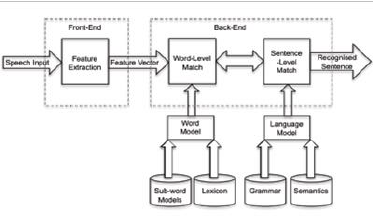
\includegraphics[width=10cm]{data_science/speech_recognition/asr_components}

Trong bước thứ nhất, trích rút thông tin \textit{Feature Extraction}, các mẫu tín hiệu được tham số hóa. Mục tiêu là trích xuất ra một tập các tham số (đặc trưng) từ tín hiệu có nhiều thông tin hữu ích nhất cho quá trình phân loại.  Các đặc trưng chính được trích xuất với điều kiện \textit{thích nghi} với các sự thay đổi của âm thanh và \textit{nhạy cảm} với các nội dung ngôn ngữ.

\definition{mô hình âm học}{Trong module phân loại, các vector đặc trưng được ánh xạ với các pattern, được gọi là \textbf{mô hình âm học} (acoustic model). Mô hình học thường là HMM được train với toàn bộ từ, hay âm như là một đơn vị ngôn ngữ.}

\definition{từ điển phát âm}{
Từ điển phát âm (pronunciation dictionary) định nghĩa cách kết hợp âm cho các ký tự. Nó có thể chứa cách phát âm khác nhau cho cùng một từ. Bảng 1 hiển thị chính xác một từ điển. Từ (graphme) ở cột bên trái ứng với cách phát âm (các âm) ở cột bên phải (các ký tự âm trong bảng được dùng phổ biến đối với tiếng Anh)
}

Ví dụ một phần của từ điển âm học tiếng Anh trong thực tế

\begin{tabular}{ | l | l | }
  \hline
  word & pronunciation \\ \hline
  INCREASE & ih n k r iy s \\ \hline
  INCREASED & ih n k r iy s t \\ \hline
  INCREASES & ih n k r iy s ah z \\ \hline
  INCREASING & ih n k r iy s ih ng  \\ \hline
  INCREASINGLY & ih n k r iy s ih ng l iy \\ \hline
  INCREDIBLE & ih n k r eh d ah b ah l \\ \hline
\end{tabular}

\definition{mô hình ngôn ngữ}{
\textit{Mô hình ngôn ngữ} (language model) chứa các thông tin về cú pháp. Mục tiêu để dự đoán khả năng một từ xuất hiện sau các từ khác trong một ngôn ngữ. Nói cách khác, xác xuất để một từ $k$ xảy ra sau khi $k-1$ từ trước đó được định nghĩa bởi $P(w_k | w_{k-1}, w_{k-2}, ..., w_1)$
}

\textbf{Mô hình hóa sub-word với HMMs}

Trong các hệ thống ASR, HMMs được dùng để biểu diễn các đơn vị dưới từ (ví dụ như âm). Với ngôn ngữ, thông thường có 40 âm. Số lượng âm phụ thuộc vào từ điển được sử dụng. Số lượng âm phụ thuộc vào từ điển được sử dụng. Mô hình từ có thể được xây dựng bằng cách kết hợp các mô hình dưới từ.

Trong thực tế, khi nhận dạng một âm phụ thuộc rất nhiều vào các âm bên cạnh. Do đó, mô hình âm phụ thuộc ngữ cảnh (*context dependence*) được sử dụng rất phổ biến. Mô hình *biphone* chú ý đến âm bên trái hoặc âm bên phải, mô hình *triphone* chú ý đến cả hai phía, với một âm, các mô hình khác nhau được sử dụng trong ngữ cảnh khác nhau. Hình dưới thể hiện các mô hình monophone, biphone và triphone của từ *bat* (b ae t)

![](http://www.igi.tugraz.at/lehre/CI/SS08/tutorials/ASR/img10.gif)

\section{Quá trình huấn luyện}

\textbf{Huấn luyện các mô hình monophone}

Một mô hình monophone là một mô hình âm học, trong đó không chứa thông tin ngữ cảnh về các âm trước và sau. Nó được sử dụng như thành phần cơ bản cho các mô hình triphone - mô hình sử dụng những thông tin về ngữ cảnh.

Việc huấn luyện sử dụng framework Gaussian Mixture Model/Hidden Markov Model.

\textbf{Dóng hàng âm thanh trong mô hình âm học}

Các tham số trong mô hình âm học được tính toán trong quá trình huấn luyện; tuy nhiên, quá trình này có thể được tối ưu hóa bởi việc lặp lại quá trình huấn luyện và dòng hàng. Còn lại là huấn luyện Viterbi (liên quan đến phương pháp này, nhưng dùng nhiều khối lượng tính toán hơn là thuật toán Forward-Backward và Expectation Maximization). Bằng cách dóng hàng âm thanh - phụ đề với mô hình âm học hiện tại, các thuật toán huấn luyện có thể sử dụng kết quả này để cải thiện và hiệu chỉnh tham số của mô hình. Do đó, mỗi quá trình huấn luyện sẽ theo bởi một bước dóng hàng trong đó âm thanh và văn bản được dóng hàng lại.

\textbf{Huấn luyện các mô hình triphone}

Trong khi các mô hình monophone đơn giản biểu diễn các đặc trưng âm thanh như một đơn âm, trong khi các âm vị sẽ thay đổi đáng kể phụ thuộc vào ngữ cảnh. Mô hình triphone thể hiện một âm trong ngữ cảnh với hai âm bên cạnh.

Đến đây, một vấn đề là không phải tất cả các đơn vị triphone được thể hiện trong dữ liệu huấn luyên. Có tất cả $\textnormal(\# of phonemes)^3$ triphone, nhưng chỉ có một tập thực sự tồn tại trong dữ liệu. Hơn nữa, các đơn vị xảy ra nhiều lần trong dữ liệu đưa ra kết quả thống kê tốt hơn trong dữ liệu. Một nhóm cây quyết định phân chia các triphones vào các nhóm, mục đích giảm thiểu tham số và đưa ra quyết định tốt hơn.

\textbf{Dóng hàng các mô hình âm học và huấn luyện lại các mô hình triphone}

Lặp lại các bước dòng hàng âm thanh và huấn luyện các mô hình triphone với các thuật toán huấn luyện để hiệu chỉnh mô hình. Các phương pháp phổ biến là delta+delta-delta, LDA-MLLT và SAT. Các giải thuật dóng hàng bao gồm dóng hàng cho từng người nói và FMLLR.

\textbf{Các thuật toán huấn luyện}

Huấn luyện delta+delta-delta tính các đặc trưng delta và double-delta, hay các hệ số động, để thêm vào các đặc trưng MFCC. Delta và delta-delta là các đặc trưng số học, tính các đạo hàm bậc 1 và 2 của tín hiệu. Do đó, phép tính toán này thường được thực hiện trên một window của các đặc trưng vector. Trong khi một window của hai đặc trưng vector có thể hiệu quả, nó là các xấp xỉ thô (giống như delta-diffrence là một xấp xỉ thô của đạo hàm). Đặc trưng delta được tính toán trong các window của các đặc trưng cơ bản, trong khi delta-delta được tính toán trong các window của đặc trựng delta.

LDA-MLLT viết tắt của Linear Discriminant Analysis - Maximum Likelihood Linear Transform. Linear Discriminant Analysis lấy các đặc trưng vector và xây dựng các trạng thái HMM, nhưng giảm thiểu không gian vector. Maximum Likelihood Linear Transfrom lấy các đặc trưng được giảm từ LDA, và thực hiện các biến đổi đối với từng người nói. MLLT sau đó thực hiện một bước chuẩn hóa, để giảm sự khác biệt giữa các người nói.

SAT viết tắt của Speaker Adaptive Training. SAT cũng thực hiện các chuẩn hóa đối với người nói bằng cách thực hiện biến đổi trên mỗi người nói. Kết quả của quá trình này đồng nhất và chuẩn hóa hơn, cho phép mô hình có thể sử dụng những tham số này để giảm thiểu sự biến đổi của âm, đối với từng người nói hoặc môi trường thu.

\textbf{Các thuật toán dóng hàng}

Thuật toán dòng hàng luôn luôn cố định, trong đó các kịch bản chấp nhận các loại đầu vào âm học khác nhau. Dòng hàng đối với từng người nói, sẽ tách biệt thông tin giữa các người nói trong quá trình dóng hàng.

fMLLR viết tắt của Feature Space Maximum Likelihood Linear Regression. Sau quá trình huấn luyện SAT, các mô hình âm học không huấn luyện trên các đặc trưng ban đầu, mà đối với các đặc trưng chuẩn hóa theo người nói. Với quá trình dóng hàng, xóa bỏ sự khác biệt giữa người nói (bằng cách nghịch đạo ma trận fMLLR), sau đó loại bỏ nó khỏi mô hình *bằng cách nhân ma trận nghịch đảo với đặc trưng vector). Mô hình âm học quasi-speaker-independent có thể sử dụng trong quá trình dóng hàng.

\textbf{Dóng hàng (Forced Alignment)}

Hệ thống nhận dạng tiếng nói sử dụng một máy tìm kiếm bên cạnh mô hình âm học và ngôn ngữ trong đó chứa tập các từ, âm và tập dữ liệu để đối chiếu với dữ liệu âm thanh cho câu nói. Máy tìm kiếm này sử dụng các đặc trưng được trích xuất bởi dữ liệu âm thanh để xác định sự xuất hiện của từ, âm và đưa ra kết quả.

![](https://www.isip.piconepress.com/projects/speech/software/tutorials/production/fundamentals/v1.0/section_04/images/srec_s04_04_p01.jpg)

Quá trình dòng hàng cũng tương tự như vậy, nhưng khác ở một điểm quan trong. Thay vì đưa vào tập các từ có thể để tìm kiếm, máy tìm kiếm đưa vào đoạn phụ đề tương ứng với câu nói. Hệ thống sau đó dóng hàng dữ liệu văn bản với dữ liệu âm thanh, xác định đoạn nào trong âm thanh tương ứng với từ cụ thể nào trong dữ liệu văn bản.

![](https://www.isip.piconepress.com/projects/speech/software/tutorials/production/fundamentals/v1.0/section_04/images/fallign_s04_04_p01.jpg)

Dóng hàng có thể sử dụng để dóng âm trong dữ liệu với bản với dữ liệu âm thanh, giống như hình dưới đây, các âm được xác định trong từng đoạn của âm thanh.

![](https://www.isip.piconepress.com/projects/speech/software/tutorials/production/fundamentals/v1.0/section_04/images/fallign2_s04_04_p01.jpg)

\section{Hidden Markov Model}

Hidden Markov Model (HMM) là mô hình trọng số với các trọng số ở cung, chỉ khả năng xuất hiện của cung.

*Một trong những ứng dụng của HMM, là phán đoán chuỗi các trạng thái thay đổi, dựa vào chuỗi các quan sát*

Các trọng số trong trạng thái gọi là observation likelihood, các trọng số ở cung gọi là transition likelihood.

Sau đây là một ví dụ:

\begin{itemize}
  \item Thời tiết trong một ngày có thể là NÓNG hoặc LẠNH
  \item Khi trời NÓNG, 20\% bạn dùng 1 viên đá, 40\% bạn dùng 2 viên, 40\% cho 3 viên.
  \item Khi trời LẠNH, 50\% bạn dùng 1 viên, 40\% bạn dùng 2, 10\% bạn dùng 3. Đây là các khả năng trong quá trình quan sát (observation likelihood)
  \item Khi trời NÓNG, 30\% nó sẽ chuyển sang LẠNH, 70\% giữ nguyên. Khi trời LẠNH, 40\% nó sẽ chuyển sang NÓNG, 60\% giữ nguyên. Đây là khả năng dịch chuyển (trainsition likelihood)
\end{itemize}

* ![https://qph.ec.quoracdn.net/main-qimg-a6744f9e17e59f3729d6fef02d54391b.webp](https://qph.ec.quoracdn.net/main-qimg-a6744f9e17e59f3729d6fef02d54391b.webp)

Giờ, giả sử chung ta quan sát trong 3 ngày, bạn dùng 1,2,3 viên đá. Thời tiết có khả năng diễn ra như thế nào?

Đến đây chúng ta dùng thuật toán Viterbi. Về cơ bản, nó là dynamic programming với hai chiều $[state, position\_in\_sequence]$

Gọi S là trạng thái hiện tại {HOT, COLD} trong quan sát i, S' là trạng thái trước đó, và A là lượng đá tiêu thụ {1, 2, 3} trong quan sát i

$$Viterbi[S,i] = Viterbi[S', i-1] * p(S|S') * p(A|S)$$
$$V[S,i] = V[S',i-1] * transition\_likelihood * observation\_likelihood$$

HMM được sử dụng trong các hệ thống thỏa mãn

\begin{enumerate}
  \item Có hữu hạn các trạng thái nội tại (internal state), là nguyên nhân của các sự kiện (external events) (các quan sát)
  \item Trạng thái nội tại không quan sát được (hidden)
  \item Trạng thái hiện tại chỉ phụ thuộc vào trạng thái trước đó (qúa trình Markov)
\end{enumerate}

Wow! George nhanh chóng liên hệ vụ của anh đấy với mô hình HMM. George nhận ra rằng CCTV footage từ các cập có thể coi như là chuỗi quan sát được, anh đấy có thể dùng mô hình và sử dụng nó để phát hiện hành vị ẩn mà Bob và William hoạt động.

\textbf{3 vấn đề cơ bản} được Jack Ferguson giới thiệu trong những năm 1960

\begin{enumerate}
  \item (Likelihood): Cho một HMM $\lambda = (A, B)$ và một chuỗi quan sát $O$, xác định likelihood $P(O|\lambda)$
  \item (Decoding): Cho một chuỗi quan sát $O$, và một HMM $\lambda = (A,B)$, xác định chuỗi ẩn $Q$ tốt nhất
  \item (Learning): Cho một chuỗi quan sát $O$, một tập các trạng thái trong HMM, học các tham số $A$ và $B$
\end{enumerate}

\section{Likelihood Computation}

Vấn đề đầu tiên là tính xác suất xảy ra của một chuỗi quan sát. Ví dụ, trong bài toán ăn đá ở hình 9.3, xác suất xảy ra chuỗi *3 1 3* là bao nhiêu?

**Tính toán Likelihood**: Chuỗi một HMM $\lambda = (A, B)$, và mỗi chuỗi quan sát $O$, xác định likelihood $P(O|\lambda)$

Thuật toán Forward, nếu sử dụng Bayes rule, để tính likelihood, cần khối lượng tính toán $N^T$ với N là số trạng thái có thể có và T là chiều dài chuỗi quan sát. Ví dụ trong bài toán gán nhãn có N=10 nhãn, chiều dài của chuỗi trung bình là 28, thì cần $10^{28}$ bước tính toán. Một giải thuật với hiệu quả $O(N^2T)$ được đề xuất với tên gọi \textbf{forward algorithm}

Tài liệu tham khảo

* http://www.igi.tugraz.at/lehre/CI/SS08/tutorials/ASR/node1.html
* https://www.isip.piconepress.com/projects/speech/software/tutorials/production/fundamentals/v1.0/section_04/s04_04_p01.html
* http://www.igi.tugraz.at/lehre/CI/SS08/tutorials/ASR/node1.html
* https://www.isip.piconepress.com/projects/speech/software/tutorials/production/fundamentals/v1.0/section_04/s04_04_p01.html
* https://www.quora.com/What-is-a-simple-explanation-of-the-Hidden-Markov-Model-algorithm

\chapter{Tổng hợp tiếng nói}

\diary{20/12/2017: Text to speech 100. Cảm ơn project rất hay của \href{https://vais.vn/vi/tai-ve/hts_for_vietnamese/}{bạn Truong Do ở vais}, nếu không có project này chắc mình phải mất rất nhiều thời gian mới có được phiên bản text to speech đầu tiên.}

Tóm lại thì việc sinh ra tiếng nói từ text gồm 4 giai đoạn

\begin{enumerate}
  \item Sinh ra features từ file wav sử dụng tool sptk
  \item Tạo một lab, trong đó có dữ liệu huấn luyện (những đặc trưng của âm thanh được trích xuất từ bước 1), text đầu vào
  \item Sử dụng htk để train dữ liệu từ thư mục lab, đầu ra là một model
  \item Sử dụng model để sinh ra output với text đầu vào, dùng hts\_engine để decode, kết quả được wav files.
\end{enumerate}

Phù. 4 bước đơn giản thế này thôi mà không biết. Lục cả internet ra mãi chẳng hiểu, cuối cùng file phân tích file `train.sh` của bạn Truong Do mới hiểu. Ahihi
%\chapter{Phân loại văn bản}

<h3>Naive Bayes Classifier</h3>
Tham khảo thư viện <a href="http://scikit-learn.org/stable/modules/naive_bayes.html" target="_blank" rel="noopener">Scikit-learn</a>

Xét bài toán classification với C classes 1,2,…,C. Tính xác suất để 1 điểm dữ liệu rơi vào class C ta có công thức: $latex P(\frac{c}{x})$. Tức tính xác suất để đầu ra là class C biết rằng đầu vào là vector x. Việc xác định class của điểm dữ liệu đó bằng cách chọn ra class có xác suất cao nhất:<p style="text-align:center;">
c = argmax($latex P(\frac{c}{x})$) với c ∈ {1,…,C}</p>
Sử dụng quy tắc Bayes:<p style="text-align:center;">
c = argmax($latex P(\frac{c}{x})$) = argmax($latex P(\frac{P(\frac{c}{x})P(x)}{P(x)}$) = argmax($latex P(\frac{P(\frac{c}{x})}{P(c)}$))</p>

<h4>Các phân phối thường dùng</h4>
<strong>Gaussian Naive Bayes</strong>
Mô hình này được sử dụng chủ yếu trong loại dữ liệu mà các thành phần là các biến liên tục.
<strong>Multinomial Naive Bayes</strong>
Mô hình này chủ yếu được sử dụng trong phân loại văn bản mà feature vectors được tính bằng Bags of Words. Lúc này, mỗi văn bản được biểu diễn bởi một vector có độ dài d chính là số từ trong từ điển. Giá trị của thành phần thứ i trong mỗi vector chính là số lần từ thứ i xuất hiện trong văn bản đó.
Khi đó, $latex P(\frac{x_i}{c})$ tỉ lệ với tần suất từ thứ i xuất hiện trong các văn bản của class c:<p style="text-align:center;"> $latex P(\frac{x_i}{c})$ = $latex \frac{Nx_i}{Nc}$</p>
<p style="padding-left:70px;">Trong đó:</p>
<p style="padding-left:90px;">$latex Nx_i$ là tổng số lần từ thứ i xuất hiện trong các văn bản của class c, nó được tính là tổng của tất cả các thành phần thứ i của các feature vectors ứng với class c.</p>
<p style="padding-left:90px;">$latex Nc$ là tổng số từ (kể cả lặp) xuất hiện trong class c. Hay bằng tổng độ dài của toàn bộ các văn bản thuộc vào class c.</p>
Nếu có một từ mới chưa bao giờ xuất hiện trong class c thì biểu thức trên sẽ bằng 0, điều này dẫn đến vế phải của c bằng 0.
<strong>Bernoulli Naive Bayes</strong>
Mô hình này được áp dụng cho các loại dữ liệu mà mỗi thành phần là một giá trị binary. Ví dụ: cũng với loại văn bản nhưng thay vì đếm tổng số lần xuất hiện của 1 từ trong văn bản, ta chỉ cần quan tâm từ đó có xuất hiện hay không.
Khi đó: $latex P(\frac{x_i}{c})$ = $latex P(\frac{i}{c})x_i$ + (1 − $latex P(\frac{i}{c})$(1 − $latex x_i $))
Với $latex P(\frac{i}{c})$ là xác suất từ thứ i xuất hiện trong các văn bản của class c.
%\chapter{Pytorch}

\diary{08/12/2017: Cảm giác \href{http://videolectures.net/deeplearning2017_chintala_torch/}{talk} của anh Soumith Chintala (Facebook, research editor) ở Deep Learning Summer School 2017 khá thú vị}

Sau khi nghe bài này thì hâm mộ luôn anh Soumith Chintala, tìm loạt bài anh trình bày luôn

* [PyTorch: Fast Differentiable Dynamic Graphs in Python with a Tensor JIT](https://www.youtube.com/watch?v=DBVLcgq2Eg0&amp;t=2s), Strange Loop Sep 2017
* [Keynote: PyTorch: Framework for fast, dynamic deep learning and scientific computing](https://www.youtube.com/watch?v=LAMwEJZqesU&amp;t=66s), EuroSciPy Aug 2017


\section{So sánh giữa Tensorflow và Pytorch?}

Có 2 điều cần phải nói khi mọi người luôn luôn so sánh giữa Tensorflow và Pytorch. (1) Tensorflow khiến mọi người "không thoải mái" (2) Pytorch thực sự là một đối thủ trên bàn cân. Một trong những câu trả lời hay nhất mình tìm được là của anh Hieu Pham (Google Brain) [trả lời trên quora (25/11/2017)](https://www.quora.com/What-are-your-reviews-between-PyTorch-and-TensorFlow/answer/Hieu-Pham-20?srid=5O2u). Điều quan trọng nhất trong câu trả lời này là *"Dùng Pytorch rất sướng cho nghiên cứu, nhưng scale lên mức business thì Tensorflow là lựa chọn tốt hơn"*

## Behind The Scene

(15/11/2017) Hôm nay bắt đầu thử nghiệm pytorch với project thần thánh classification sử dụng cnn https://github.com/Shawn1993/cnn-text-classification-pytorch

Cảm giác đầu tiên là make it run khá đơn giản

```
conda create -n test-torch python=3.5
pip install http://download.pytorch.org/whl/cu80/torch-0.2.0.post3-cp35-cp35m-manylinux1_x86_64.whl
pip install torchvision
pip install torchtext
```

Thế là `main.py` chạy! Hay thật. Còn phải vọc để bạn này chạy với CUDA nữa.

**Cài đặt CUDA trong ubuntu 16.04**

Kiểm tra VGA

```
$ lspci | grep VGA
01:00.0 VGA compatible controller: NVIDIA Corporation GM204 [GeForce GTX 980] (rev a1)
```

Kiểm tra CUDA đã cài đặt trong Ubuntu [^1]

```
$ nvcc --version
nvcc: NVIDIA (R) Cuda compiler driver
Copyright (c) 2005-2016 NVIDIA Corporation
Built on Sun_Sep__4_22:14:01_CDT_2016
Cuda compilation tools, release 8.0, V8.0.44
```

Kiểm tra pytorch chạy với cuda `test_cuda.py`

```python
import torch
print("Cuda:", torch.cuda.is_available())
```

```
$ python test_cuda.py
CUDA: True
```

Chỉ cần cài đặt thành công CUDA là pytorch tự work luôn. Ngon thật!

*Ngày X*

Chẳng hiểu sao update system kiểu nào mà hôm nay lại không sử dụng được CUDA `torch.cuda.is_available() = False`. Sau khi dùng lệnh `torch.Tensor().cuda()` thì gặp lỗi

```
AssertionError:
The NVIDIA driver on your system is too old (found version 8000).
Please update your GPU driver by downloading and installing a new
version from the URL: http://www.nvidia.com/Download/index.aspx
Alternatively, go to: https://pytorch.org/binaries to install
a PyTorch version that has been compiled with your version
of the CUDA driver.
```

Kiểm tra lại thì mình đang dùng nvidia-361, làm thử theo [link này](http://www.linuxandubuntu.com/home/how-to-install-latest-nvidia-drivers-in-linux) để update NVIDIA, chưa biết kết quả ra sao?

May quá, sau khi update lên nvida-387 là ok. Haha

**Ngày 2**

Hôm qua đã bắt đầu implement một nn với pytorch rồi. Hướng dẫn ở [Deep Learning with PyTorch: A 60 Minute Blitz](http://pytorch.org/tutorials/beginner/deep_learning_60min_blitz.html) hữu ích phết.

Hướng dẫn implement các mạng neural với pytorch rất hay tại [PyTorch-Tutorial](https://github.com/MorvanZhou/PyTorch-Tutorial)

(lượm lặt) Trang này [Awesome-pytorch-list](https://github.com/bharathgs/Awesome-pytorch-list) chứa rất nhiều link hay về pytorch như tập hợp các thư viện liên quan, các hướng dẫn và ví dụ sau đó là các cài đặt của các paper sử dụng pytorch.

(lượm lặt) Loạt video hướng dẫn pytorch [PyTorchZeroToAll](https://www.youtube.com/watch?v=SKq-pmkekTk&amp;list=PLlMkM4tgfjnJ3I-dbhO9JTw7gNty6o_2m) của tác giả Sung Kim trên youtube.

Bước tiếp theo là visualize loss và graph trong tensorboard, sử dụng [tensorboard_logger](https://github.com/TeamHG-Memex/tensorboard_logger) khá hay.

```
pip install tensorboard_logger
pip install tensorboard
```

Chạy tensorboard server

```
tensorboard --log-dir=runs
```

**Ngày 3**: Vấn đề kỹ thuật

Hôm qua cố gắng implement một phần thuật toán CNN cho bài toán phân lớp văn bản. Vấn đề đầu tiên là biểu diển sentence thế nào. Cảm giác load word vector vào khá chậm. Mà thằng tách từ của underthesea cũng chậm kinh khủng.

Một vài link tham khảo về bài toán CNN: [Implementing a CNN for Text Classification in TensorFlow](http://www.wildml.com/2015/12/implementing-a-cnn-for-text-classification-in-tensorflow/), [Text classification using CNN : Example](https://agarnitin86.github.io/blog/2016/12/23/text-classification-cnn)

[^1]: https://askubuntu.com/questions/799184/how-can-i-install-cuda-on-ubuntu-16-04


%\chapter{Big Data}

View online \href{http://magizbox.com/training/bigdata/site/}{http://magizbox.com/training/bigdata/site/}

Big Data Q&A
1. What is "Big Data"? 1
https://www.youtube.com/watch?v=TzxmjbL-i4Y

2. How big is big data? 2


3. How much data is "Big Data"? 3


4. What are characteristics of "Big Data"? 4


5. What is big data ecosystem? 5


6. What is big data landscape 6


7. What are benefits of big data? 7


https://www.youtube.com/watch?v=TzxmjbL-i4Y ↩ ↩

http://scoop.intel.com/what-happens-in-an-internet-minute/ ↩ ↩

http://www.quora.com/How-much-data-is-Big-Data ↩ ↩

https://en.wikipedia.org/wiki/Big_data#Characteristics ↩ ↩

http://www.clearpeaks.com/blog/big-data/big-data-ecosystem-spark-and-tableau ↩ ↩

https://vladimerbotsvadze.wordpress.com/2015/01/28/the-big-data-landscape-technology-businessintelligence-analytics/ ↩ ↩

http://blog.galaxyweblinks.com/big-data-with-bigger-benefits/ ↩ ↩

\section{Distribution Storage}

\subsection{HDFS}

The Hadoop Distributed File System (HDFS) — a subproject of the Apache Hadoop project—is a distributed, highly fault-tolerant file system designed to run on low-cost commodity hardware. HDFS provides high-throughput access to application data and is suitable for applications with large data sets. This article explores the primary features of HDFS and provides a high-level view of the HDFS architecture.
: sequenceiq/hadoop-docker

Big Data Stack: HDFS, Kibana, ElasticSearch, Neo4J, Apache Spark

\subsection{HBase}

Apache HBase™ is the Hadoop database, a distributed, scalable, big data store. Download Apache HBase™ Click here to download Apache HBase™.


1. When Would I Use Apache HBase? 1
HBase isn’t suitable for every problem.

First, make sure you have enough data. If you have hundreds of millions or billions of rows, then HBase is a good candidate. If you only have a few thousand/million rows, then using a traditional RDBMS might be a better choice due to the fact that all of your data might wind up on a single node (or two) and the rest of the cluster may be sitting idle.

Second, make sure you can live without all the extra features that an RDBMS provides (e.g., typed columns, secondary indexes, transactions, advanced query languages, etc.) An application built against an RDBMS cannot be "ported" to HBase by simply changing a JDBC driver, for example. Consider moving from an RDBMS to HBase as a complete redesign as opposed to a port.

Third, make sure you have enough hardware. Even HDFS doesn’t do well with anything less than 5 DataNodes (due to things such as HDFS block replication which has a default of 3), plus a NameNode.

HBase can run quite well stand-alone on a laptop - but this should be considered a development configuration only.

2. Features 2
Linear and modular scalability.
Strictly consistent reads and writes.
Automatic and configurable sharding of tables
Automatic failover support between RegionServers.
Convenient base classes for backing Hadoop MapReduce jobs with Apache HBase tables.
Easy to use Java API for client access.
Block cache and Bloom Filters for real-time queries.
Query predicate push down via server side Filters
Thrift gateway and a REST-ful Web service that supports XML, Protobuf, and binary data encoding options
Extensible jruby-based (JIRB) shell
Support for exporting metrics via the Hadoop metrics subsystem to files or Ganglia; or via JMX
3. Architecture


HBase Shell
[code lang="shell"]

list all table
list [/code]

Up & Running
1. Download
HBase 0.94.27 (HBase 0.98 won't work)

[code lang="shell"] wget https://www.apache.org/dist/hbase/hbase-0.94.27/hbase-0.94.27.tar.gz tar -xzf hbase-0.94.27.tar.gz [/code]

2. Setup
1. edit $HBASE_ROOT/conf/hbase-site.xml and add

[code lang="xml"] hbase.rootdir file:///full/path/to/where/the/data/should/be/stored hbase.cluster.distributed false [/code]

3. Verify
Go to http://localhost:60010 to see if HBase is running.

When Should I Use HBase? ↩
HBase ↩
Config HBase Remote
1. Change /etc/hosts
[code] 127.0.0.1 [username] [server_ip] hbase.io [/code]

Example

[code] 127.0.0.1 crawler 192.168.0.151 hbase.io [/code]

2. Change hostname
[code] hostname hbase.io [/code]

3. Change region servers
Edit $HBASE_ROOT/conf/regionservers

[code] hbase.io [/code]

4. Change $HABSE_ROOT/conf/hbase-site.xml
[code lang="xml" title="hbase-site.xml"] <?xml-stylesheet type="text/xsl" href="configuration.xsl"?> hbase.rootdir file:///home/username/Downloads/hbase/data hbase.cluster.distributed false hbase.zookeeper.quorum hbase.io zookeeper.znode.parent /hbase-unsecure hbase.rpc.timeout 2592000000 [/code]

Docker
HBase 0.94

Image: https://github.com/Banno/docker-hbase-standalone

[code] docker run -d -p 2181:2181 -p 60000:60000 -p 60010:60010 -p 60020:60020 -p 60030:60030 banno/hbase-standalone [/code]

Compose

[code] hbase.vmware: build: ./docker-hbase-standalone/. command: "/opt/hbase/hbase-0.94.15-cdh4.7.0/bin/hbase master start" hostname: hbase.vmware ports: - 2181:2181 - 60000:60000 - 60010:60010 - 60020:60020 - 60030:60030 volumes: - ./docker-hbase-standalone/hbase-0.94.15-cdh4.7.0:/opt/hbase/hbase-0.94.15-cdh4.7.0 - ./data/hbase:/tmp/hbase-root/hbase /code]

\section{Distribution Computing}

\subsection{Apache Spark}




Apache Spark is an open-source cluster computing framework originally developed in the AMPLab at UC Berkeley. In contrast to Hadoop's two-stage disk-based MapReduce paradigm, Spark's in-memory primitives provide performance up to 100 times faster for certain applications. By allowing user programs to load data into a cluster's memory and query it repeatedly, Spark is well-suited to machine learning algorithms.
Installation
Requirements: Hadoop, YARN

Install Hadoop

Insatll YARN

Install Java

Verification
Tutorial
From Pandas to Apache Spark’s DataFrame

Big Data Stack: HDFS, Kibana, ElasticSearch, Neo4J, Apache Spark

Apache Spark: Tutorials
Beginners Guide: Apache Spark Machine Learning with Large Data


Spark and Spark Streaming Unit Testing Recipes for Running Spark Streaming Applications in Production- Databricks

Spark Streaming


Spark and Spark Streaming Unit Testing Recipes for Running Spark Streaming Applications in Production- Databricks

\section{Components}

\subsection{Ambari}

The Apache Ambari project is aimed at making Hadoop management simpler by developing software for provisioning, managing, and monitoring Apache Hadoop clusters. Ambari provides an intuitive, easy-to-use Hadoop management web UI backed by its RESTful APIs.

Ambari enables System Administrators to:

Provision a Hadoop Cluster

Ambari provides a step-by-step wizard for installing Hadoop services across any number of hosts.
Ambari handles configuration of Hadoop services for the cluster.
Manage a Hadoop Cluster

Ambari provides central management for starting, stopping, and reconfiguring Hadoop services across the entire cluster.
Monitor a Hadoop Cluster

Ambari provides a dashboard for monitoring health and status of the Hadoop cluster.
Ambari leverages Ambari Metrics System for metrics collection.
Ambari leverages Ambari Alert Framework for system alerting and will notify you when your attention is needed (e.g., a node goes down, remaining disk space is low, etc).
Ambari enables Application Developers and System Integrators to:

Easily integrate Hadoop provisioning, management, and monitoring capabilities to their own applications with the Ambari REST APIs.
Docker


Receipts:

Image: sequenceiq/ambari (git)
Multinode cluster with Ambari 1.7.0 1
Get the docker images

[code] docker pull sequenceiq/ambari:1.7.0 [/code]

Get ambari-functions [code] curl -Lo .amb j.mp/docker-ambari-170 && . .amb [/code]

Create your cluster – automated

[code] amb-deploy-cluster 3 [/code]

Multinode cluster with Ambari 1.7.0 ↩

\subsection{Kibana}

Kibana is an open source data visualization plugin for Elasticsearch. It provides visualization capabilities on top of the content indexed on an Elasticsearch cluster. Users can create bar, line and scatter plots, or pie charts and maps on top of large volumes of data.

\subsection{Logstash}

https://www.digitalocean.com/community/tutorials/how-to-use-logstash-and-kibana-to-centralize-logs-on-centos-6

\subsection{Elasticsearch}


Elasticsearch is a search server based on Lucene. It provides a distributed, multitenant-capable full-text search engine with a RESTful web interface and schema-free JSON documents. Elasticsearch is developed in Java and is released as open source under the terms of the Apache License. Elasticsearch is the second most popular enterprise search engine
1. Basic Concenpts
Relational Database	Elasticsearch
Database	Index
Table	Type
Row	Document
Column	Field
Schema	Mapping
2. Index & Query
Get all indices
/_stats
Search API 1
Search All
/bank/_search?q=*
hits.hits – actual array of search results (defaults to first 10 documents)

Query Language
elasticsearch provides a full Query DSL based on JSON to define queries.

curl -XPOST /bank/_search
// match all, limit 10 offset 10
{
  "query": { "match_all": {} },
  "from": 10,
  "size": 10
}

// select fields
{
  "query": { "match_all": {} },
  _source: ["account_number", "balance"]
  "size": 10
}

// where account equals 20
{
  "query": { "match": { "account_number": 20 } }
}
Filter

curl -XPOST elastic:9200/index/type/_search -d '
{
  "query" : {
    "filtered" :
    {
      "query" : { "term" : { "feature" : 1 } } ,
      "filter" : {
        "and" : [
          {
            "range": {
              "_timestamp": {
                "from": 1441964671000,
                "to": 1441964672000
              }
            }
          }
        ]
      }
    }
  }
}
Sort

curl -XPOST elastic:9200/index/type/_search -d '
{
  "query" : {
    "filtered" :
    {
      "query" : { "term" : { "feature" : 1 } } ,
      "filter" : {
        "and" : [
          {
            "range": {
              "_timestamp": {
                "from": 1441964671000,
                "to": 1441964672000
              }
            }
          }
        ]
      }
    }
  }
}
3. Mapping
Timestamp 2
Enable and store timestamp

curl -XPOST localhost:9200/test
{
"mappings" : {
    "_default_":{
        "_timestamp" : {
            "enabled" : true,
            "store" : true
        }
    }
  }
}'
Relationships Management 3 4
Inner Object

👍 Easy, fast, performant
👎 No need for special queries
☛ Only applicable when one-to-one relationships are maintained
Nested

👍 Nested docs are stored in the same Lucene block as each other, which helps read/query performance. Reading a nested doc is faster than the equivalent parent/child.
👎 Updating a single field in a nested document (parent or nested children) forces ES to reindex the entire nested document. This can be very expensive for large nested docs
👎 “Cross referencing” nested documents is impossible
☛ Best suited for data that does not change frequently
Parent/Child

👍 Updating a child doc does not affect the parent or any other children, which can potentially save a lot of indexing on large docs
👎 Children are stored separately from the parent, but are routed to the same shard. So parent/children are slightly less performance on read/query than nested
👎 Parent/child mappings have a bit extra memory overhead, since ES maintains a “join” list in memory
👎 Sorting/scoring can be difficult with Parent/Child since the Has Child/Has Parent operations can be opaque at times
Denormalization

👍 You get to manage all the relations yourself!
👎 Most flexible, most administrative overhead
☛ May be more or less performant depending on your setup
4. Backup
Elastic Dump 5
Tools for moving and saving indicies.

bin/elasticdump
  --input=http://localhost:9200/index_1
  --output=http://localhost:9200/index_1_backup
  --type=data
  --scrollTime=100
Alias 6
curl -XPOST 'http://localhost:9200/_aliases' -d '
{
    &quot;actions&quot; : [
        { &quot;remove&quot; : { &quot;index&quot; : &quot;test1&quot;, &quot;alias&quot; : &quot;alias1&quot; } },
        { &quot;add&quot; : { &quot;index&quot; : &quot;test1&quot;, &quot;alias&quot; : &quot;alias2&quot; } }
    ]
}'
5. Module Scripting 7
Ranking
Rank #2 from DB-Engines Ranking of Search Engines

The Search API ↩
http://stackoverflow.com/a/17146144/772391 ↩
http://stackoverflow.com/a/23407367/772391 ↩
https://www.elastic.co/guide/en/elasticsearch/guide/current/modeling-your-data.html ↩
https://github.com/taskrabbit/elasticsearch-dump ↩
https://www.elastic.co/guide/en/elasticsearch/reference/current/indices-aliases.html ↩
https://www.elastic.co/guide/en/elasticsearch/reference/current/modules-scripting.html ↩
Elasticsearch tutorial series 1: Metric Aggregations with Social Network Data
Table of content

Avg, Max, Min, Sum Aggregation
Cardinality Aggregation
Stats Aggregation
Extended Stats Aggregation
Percentile Aggregation
Percentile Ranks Aggregation
Top hits Aggregation
Avg, Max, Min, Sum, Count Aggregation
Doc: Avg Aggregation, Doc: Max Aggregation, Doc: Min Aggregation

Get max, min, avg, sum, count about number of likes, shares, comments

Request

POST /facebook_crawler/post/_search
{"aggs":{"sum_like":{"sum":{"field":"num_like"}},"min_like":{"min":{"field":"num_like"}},"avg_like":{"avg":{"field":"num_like"}},"max_like":{"max":{"field":"num_like"}},"sum_share":{"sum":{"field":"num_share"}},"min_share":{"min":{"field":"num_share"}},"avg_share":{"avg":{"field":"num_share"}},"max_share":{"max":{"field":"num_share"}},"sum_comment":{"sum":{"field":"num_comment"}},"min_comment":{"min":{"field":"num_comment"}},"avg_comment":{"avg":{"field":"num_comment"}},"max_comment":{"max":{"field":"num_comment"}}}}
Request

{
"aggregations": {
      "avg_comment": {
         "value": 75.23860589812332
      },
      "min_like": {
         "value": 0
      },
      "avg_like": {
         "value": 1761974365266098.2
      },
      "sum_like": {
         "value": 3238508883359088600
      },
      "max_share": {
         "value": 30407
      },
      "max_comment": {
         "value": 11000
      },
      "sum_share": {
         "value": 117844
      },
      "max_like": {
         "value": 2751488761761411000
      },
      "avg_share": {
         "value": 250.19957537154988
      },
      "sum_comment": {
         "value": 28064
      },
      "min_comment": {
         "value": 2
      },
      "min_share": {
         "value": 1
      }
   }
}
Cardinality Aggregation
Cardinality Aggregation

Get total of users

Request

POST /facebook_crawler/post/_search
{
    "aggs" : {
        "num_authors" : { "cardinality" : { "field" : "from.fb_id" } }
    }
}
Response

{
   "aggregations": {
      "num_authors": {
         "value": 7385
      }
   }
}
Stats Aggregation
Doc: Stats Aggregation

Basic Stats of like, share & comment

Request

POST /facebook_crawler/post/_search
{
    "aggs" : {
        "shares" : { "stats" : { "field" : "num_share" } },
        "likes" : { "stats" : { "field" : "num_like" } },
        "comments" : { "stats" : { "field" : "num_comment" } }
    }
}
Response

{
   "aggregations": {
      "shares": {
         "count": 471,
         "min": 1,
         "max": 30407,
         "avg": 250.19957537154988,
         "sum": 117844
      },
      "comments": {
         "count": 373,
         "min": 2,
         "max": 11000,
         "avg": 75.23860589812332,
         "sum": 28064
      },
      "likes": {
         "count": 1838,
         "min": 0,
         "max": 2751488761761411000,
         "avg": 1761974365266098.2,
         "sum": 3238508883359088600
      }
   }
}
Extended Stats Aggregation
Extended Stats Aggregation

Stats of like, share & comment with more metrics, such as sum, std_deviation, std_deviation_bounds, variance

Request

POST /facebook_crawler/post/_search
{
    "aggs" : {
        "like_stats" : { "extended_stats" : { "field" : "num_like" } },
        "share_stats" : { "extended_stats" : { "field" : "num_share" } },
        "comment_stats" : { "extended_stats" : { "field" : "num_comment" } }
    }
}
Response

{
   "aggregations": {
      "like_stats": {
         "count": 1838,
         "min": 0,
         "max": 2751488761761411000,
         "avg": 1761974365266098.2,
         "sum": 3238508883359088600,
         "sum_of_squares": 7.667542671405507e+36,
         "variance": 4.168572634260795e+33,
         "std_deviation": 64564484310345070,
         "std_deviation_bounds": {
            "upper": 130890942985956240,
            "lower": -127366994255424050
         }
      },
      "share_stats": {
         "count": 471,
         "min": 1,
         "max": 30407,
         "avg": 250.19957537154988,
         "sum": 117844,
         "sum_of_squares": 1769467022,
         "variance": 3694230.367812983,
         "std_deviation": 1922.0380765773043,
         "std_deviation_bounds": {
            "upper": 4094.2757285261587,
            "lower": -3593.8765777830586
         }
      },
      "comment_stats": {
         "count": 373,
         "min": 2,
         "max": 11000,
         "avg": 75.23860589812332,
         "sum": 28064,
         "sum_of_squares": 131531392,
         "variance": 346970.2299304962,
         "std_deviation": 589.0417896299856,
         "std_deviation_bounds": {
            "upper": 1253.3221851580945,
            "lower": -1102.844973361848
         }
      }
   }
}
Percentiles Aggregation
Doc: Percentiles Aggregation

Comment, Like, Share Percentiles

Request

POST /facebook_crawler/post/_search
{"aggs":{"like_percentiles":{"percentiles":{"field":"num_like"}},"share_percentiles":{"percentiles":{"field":"num_share"}},"comment_percentiles":{"percentiles":{"field":"num_comment"}}}}
Response

{
"aggregations": {
      "like_percentiles": {
         "values": {
            "1.0": 0,
            "5.0": 0,
            "25.0": 4,
            "50.0": 18.35,
            "75.0": 72.53579545454545,
            "95.0": 71343.74999999999,
            "99.0": 4338260523723.276
         }
      },
      "comment_percentiles": {
         "values": {
            "1.0": 2,
            "5.0": 2,
            "25.0": 5,
            "50.0": 10,
            "75.0": 26,
            "95.0": 139.39999999999998,
            "99.0": 1000
         }
      },
      "share_percentiles": {
         "values": {
            "1.0": 1,
            "5.0": 1,
            "25.0": 1,
            "50.0": 4,
            "75.0": 25,
            "95.0": 251.5,
            "99.0": 5560.3
         }
      }
   }
}
Like Percentiles with custom percents

Request

POST /facebook_crawler/post/_search
{
   "aggs": {
      "share_percentiles": {
         "percentiles": {
            "field": "num_share",
            "percents": [0, 10, 80, 90, 95]
         }
      }
   }
}
Response

{
   "aggregations": {
      "share_percentiles": {
         "values": {
            "0.0": 1,
            "10.0": 1,
            "80.0": 37.33333333333333,
            "90.0": 97,
            "95.0": 251.5
         }
      }
   }
}
Percentile Ranks Aggregation
Doc: Percentile Ranks Aggregation

How like, share, comment distribute

Request

POST /facebook_crawler/post/_search
{
   "aggs": {
      "like_percentile_ranks": {
         "percentile_ranks": {
            "field": "num_like",
            "values": [10, 100, 1000, 10000, 1000000, 10000000]
         }
      },
      "share_percentile_ranks": {
         "percentile_ranks": {
            "field": "num_share",
            "values": [10, 100, 1000, 10000, 1000000, 10000000]
         }
      },
      "comment_percentile_ranks": {
         "percentile_ranks": {
            "field": "num_comment",
            "values": [10, 100, 1000, 10000, 1000000, 10000000]
         }
      }
   }
}
Response

{
   "aggregations": {
      "share_percentile_ranks": {
         "values": {
            "10.0": 60.438782731776364,
            "100.0": 89.91507430997878,
            "1000.0": 97.37406386327386,
            "10000.0": 99.31579836222765,
            "1000000.0": 100,
            "1.0E7": 100
         }
      },
      "like_percentile_ranks": {
         "values": {
            "10.0": 39.281828073993466,
            "100.0": 79.39530545624125,
            "1000.0": 90.98349676683587,
            "10000.0": 94.14527905373414,
            "1000000.0": 95.9014681663581,
            "1.0E7": 96.57661015941164
         }
      },
      "comment_percentile_ranks": {
         "values": {
            "10.0": 49.865951742627345,
            "100.0": 92.18395545473294,
            "1000.0": 98.92761394101876,
            "10000.0": 99.56773202397807,
            "1000000.0": 100,
            "1.0E7": 100
         }
      }
   }
}
As we can see, only 0.7% posts have more than 10k shares, onley 0.04% posts have more than 10k comment, but there is an odd here. 4.1% posts have more than 1M like (WHAT!!!). We can spot some strange here.

Top hits Aggregation
Doc: Top hits Aggregation

Example

Request

Response

{

An Aggregation
Doc: Link

Config
elasticsearch.yml

discovery.zen.minimum_master_nodes: 1
discovery.zen.ping.multicast.enabled: false
discovery.zen.ping.unicast.hosts: ["localhost"]

network.host: 0.0.0.0
http.cors.enabled: true
http.cors.allow-origin: '*'
script.inline: on
script.indexed: on
Docker
Image

https://hub.docker.com/r/_/elasticsearch/

Run

docker run -d -v "$PWD/esdata":/usr/share/elasticsearch/data elasticsearch
Docker Folder

elasticsearch/
├── config
│   └── elasticsearch.yml
└── Dockerfile
Dockerfile

FROM elasticsearch:2.2.0

ADD config/elasticsearch.yml /elasticsearch/config/elasticsearch.yml
Compose

elasticsearch:
    build: ./elasticsearch/.
    ports:
       - 9200:9200
       - 9300:9300
    volumes:
       - ./data/elasticsearch:/usr/share/elasticsearch/data
Elasticsearch: Search Ignore Accents
The ICU 1 2 analysis plug-in for Elasticsearch uses the International Components for Unicode (ICU) libraries to provide a rich set of tools for dealing with Unicode. These include the icu_tokenizer, which is particularly useful for Asian languages, and a number of token filters that are essential for correct matching and sorting in all languages other than English.

Step 1: Install ICU-Plugin 3
cd /usr/share/elasticsearch
sudo bin/plugin install analysis-icu
Step 2: Create an analyzer setting:
"settings": {
      "analysis": {
         "analyzer": {
            "vnanalysis": {
               "tokenizer": "icu_tokenizer",
               "filter": [
                  "icu_folding",
                  "icu_normalizer"
               ]
            }
         }
      }
   }
Step 3: Create your index, create a field with type string and analyzer is vnanalysis you have created
"key": {
     "type": "string",
     "analyzer": "vnanalysis"
}
Step 4: Search with sense
POST /your_index/your_doc_type/_search
{
   "query": {
      "match": {
         "key": "kiem tra"
      }
   }
}
ES: Import CSV to Elasticsearch
https://gist.github.com/clemsos/8668698

Install lastest Elasticdump with NVM
As a matter of best practice we’ll update our packages:

apt-get update
The build-essential package should already be installed, however, we’re going still going to include it in our command for installation:

apt-get install build-essential libssl-dev
To install or update nvm, you can use the install script using cURL:

curl -o- https://raw.githubusercontent.com/creationix/nvm/v0.31.0/install.sh | bash
if you have below problem or after you type nvm ls-remote command it result N/A: curl: (77) error setting certificate verify locations: CAfile: /etc/pki/tls/certs/ca-bundle.crt CApath: none

head to this 1:

or Wget:

wget -qO- https://raw.githubusercontent.com/creationix/nvm/v0.31.0/install.sh | bash
Don't forget to restart your terminal

Then you use the following command to list available versions of nodejs

nvm ls-remote
To download, compile, and install the latest v5.0.x release of node, do this:

nvm install 5.0
And then in any new shell just use the installed version:

nvm use 5.0
Or you can just run it:

nvm run 5.0 --version
Or, you can run any arbitrary command in a subshell with the desired version of node:

nvm exec 4.2 node --version
You can also get the path to the executable to where it was installed:

nvm which 5.0
Node Version Manager

how to solve https problem ↩

ICU plug-in Github ↩

Installing the ICU plug-in ↩

\subsection{Neo4J}

version: 2.3.1

Neo4j is an open-source graph database, implemented in Java. The developers describe Neo4j as "embedded, disk-based, fully transactional Java persistence engine that stores data structured in graphs rather than in tables". Neo4j is the most popular graph database.

Installation

Docker
Docker Image: https://hub.docker.com/r/library/neo4j/

Run these below command to open neo4j

# clone datahub project
git clone https://github.com/magizbox/datahub.git

# change folder to datahub directory
cd datahub

# set your config in docker-compose.yml

# run docker
docker-compose up

Cypher

Schema Discovery
List all nodes label, list all relation type

> START n=node(*) RETURN distinct labels(n)

> match n-[r]-() return distinct type(r)
UI Way: Click to Overtab in Neo4j Browser

Sample 10 entities
> MATCH (n:Entity) RETURN n, rand() as random ORDER BY random LIMIT 10
Group By
http://www.markhneedham.com/blog/2013/02/17/neo4jcypher-sql-style-group-by-functionality/

Graph Algorithms

shortestPath, dijkstra

POST http://localhost:7474/db/data/node/72/paths

Headers
Accept: application/json
Authorization: Basic bmVvNGo6cGFzc3dk

Body
{
  "to" : "http://localhost:7474/db/data/node/77",
  "max_depth" : 5,
  "relationships" : {
    "type" : "FRIEND",
    "direction" : "out"
  },
  "algorithm" : "shortestPath"
}
Graph Analystic

pagerank, closeness_centrality, betweenness_centrality, triangle_count, connected_components, strongly_connected_components

Client

In this article you will know how to connect to neo4j database from python.

Python Client
We can use Py2neo to connect to neo4j from python.

Py2neo is a client library and comprehensive toolkit for working with Neo4j from within Python applications and from the command line. The core library has no external dependencies and has been carefully designed to be easy and intuitive to use.

Snippets to connect, create, add nodes, add relationship and update property

from py2neo import authenticate, Graph, Node, Relationship
# connect to graph
authenticate("localhost:7474", "neo4j", "passwd")
graph = Graph("http://localhost:7474/db/data/")

# create unique
graph.schema.create_uniqueness_constraint('Person', 'name')

# add nodes
graph.create(Node.cast('Person', {"name": "Alice"}))
graph.create(Node.cast('Person', {"name": "Bob"}))

# add relationship
source = graph.merge_one("Person", "name", "Alice")
target = graph.merge_one("Person", "name", "Bob")
graph.create_unique(Relationship(source, "FRIEND", target))

# update property
alice = graph.merge_one("Person", "name", "Alice")
alice["age"] = 30
alice.push()

\section{Web Crawling}

\subsection{Introduction}

Web Crawler
Static Crawler

Apache Nutch
Dynamic Crawler

nutch-selenium
Intelligent Extractor

boilerpipe
Web Content Extraction Through Machine Learning
Priority Crawler, Social Crawler

Features a crawler must provide
We list the desiderata for web crawlers in two categories: features that web crawlers must provide, followed by features they should provide.

Robustness:

The Web contains servers that create spider traps, which are generators of web pages that mislead crawlers into getting stuck fetching an infinite number of pages in a particular domain. Crawlers must be designed to be resilient to such traps. Not all such traps are malicious; some are the inadvertent side-effect of faulty website development.

Politeness:

Web servers have both implicit and explicit policies regulating the rate at which a crawler can visit them. These politeness policies must be respected.

Features a crawler should provide
Distributed The crawler should have the ability to execute in a distributed fashion across multiple machines.

Scalable

The crawler architecture should permit scaling up the crawl rate by adding extra machines and bandwidth.

Performance and efficiency

The crawl system should make efficient use of various system resources including processor, storage and network bandwidth.

Quality

Given that a significant fraction of all web pages are of poor utility for serving user query needs, the crawler should be biased towards fetching ``useful'' pages first.

Freshness

In many applications, the crawler should operate in continuous mode: it should obtain fresh copies of previously fetched pages. A search engine crawler, for instance, can thus ensure that the search engine's index contains a fairly current representation of each indexed web page. For such continuous crawling, a crawler should be able to crawl a page with a frequency that approximates the rate of change of that page.

Extensible

Crawlers should be designed to be extensible in many ways - to cope with new data formats, new fetch protocols, and so on. This demands that the crawler architecture be modular.

Crawling
The basic operation of any hypertext crawler (whether for the Web, an intranet or other hypertext document collection) is as follows.

The crawler begins with one or more URLs that constitute a seed set. It picks a URL from this seed set, then fetches the web page at that URL.
The fetched page is then parsed, to extract both the text and the links from the page (each of which points to another URL).
The extracted text is fed to a text indexer.
The extracted links (URLs) are then added to a URL frontier, which at all times consists of URLs whose corresponding pages have yet to be fetched by the crawler.
Initially, the URL frontier contains the seed set; as pages are fetched, the corresponding URLs are deleted from the URL frontier. The entire process may be viewed as traversing the web graph. In continuous crawling, the URL of a fetched page is added back to the frontier for fetching again in the future.
This seemingly simple recursive traversal of the web graph is complicated by the many demands on a practical web crawling system: the crawler has to be distributed, scalable, efficient, polite, robust and extensible while fetching pages of high quality. We examine the effects of each of these issues. Our treatment follows the design of the Mercator crawler that has formed the basis of a number of research and commercial crawlers. As a reference point, fetching a billion pages (a small fraction of the static Web at present) in a month-long crawl requires fetching several hundred pages each second. We will see how to use a multi-threaded design to address several bottlenecks in the overall crawler system in order to attain this fetch rate.

Before proceeding to this detailed description, we reiterate for readers who may attempt to build crawlers of some basic properties any non-professional crawler should satisfy:

Only one connection should be open to any given host at a time.
A waiting time of a few seconds should occur between successive requests to a host.
Politeness restrictions should be obeyed.

A New Approach to Dynamic Crawler
Build a crawler system for dynamic websites is not easy task. While you can use a web browser automator (like selenium), or event when you can integrate selenium with nutch (by using nutch-selenium). These solutions are still hard to develop, hard to test and hard to manage sessions because we still "translate" our process to languages (such as java or python)

I suppose a new approach for this problem. Instead of using a web browser automator, we can inject native javascript codes into browser (via extension or add-on).The advantages of this approach is we can easily inject third party libraries (like jquery (for dom selector), Run.js (for complicated process) and APIs that supported by browsers). And we can take advance of debugging tool and testing framework in javascript world.

If you want to know about more details, feel free to contact me.

\subsection{Scrapy}

Scrapy
An open source and collaborative framework for extracting the data you need from websites. In a fast, simple, yet extensible way.

Build and run your web spiders
$ pip install scrapy
$ cat > myspider.py <<EOF
import scrapy

class BlogSpider(scrapy.Spider):
    name = 'blogspider'
    start_urls = ['https://blog.scrapinghub.com']

    def parse(self, response):
        for title in response.css('h2.entry-title'):
            yield {'title': title.css('a ::text').extract_first()}

        next_page = response.css('div.prev-post > a ::attr(href)').extract_first()
        if next_page:
            yield scrapy.Request(response.urljoin(next_page), callback=self.parse)
EOF
$ scrapy runspider myspider.py
Deploy them to Scrapy Cloud
$ shub login
Insert your Scrapinghub API Key: <API_KEY>

# Deploy the spider to Scrapy Cloud

$ shub deploy

# Schedule the spider for execution
 shub schedule blogspider
Spider blogspider scheduled, watch it running here:
https://app.scrapinghub.com/p/26731/job/1/8

# Retrieve the scraped data
$ shub items 26731/1/8
{"title": "Improved Frontera: Web Crawling at Scale with Python 3 Support"}
{"title": "How to Crawl the Web Politely with Scrapy"}
...

\subsection{Apache Nutch}

Highly extensible, highly scalable Web crawler 1 Nutch is a well matured, production ready Web crawler. Nutch 1.x enables fine grained configuration, relying on Apache Hadoop™ data structures, which are great for batch processing.

History


Usecases


1. Features 1
1. Transparency Nutch is open source, so anyone can see how the ranking algorithms work. With commercial search engines, the precise details of the algorithms are secret so you can never know why a particular search result is ranked as it is. Furthermore, some search engines allow rankings to be based on payments, rather than on the relevance of the site's contents. Nutch is a good fit for academic and government organizations, where the perception of fairness of rankings may be more important.

2. Understanding We don't have the source code to Google, so Nutch is probably the best we have. It's interesting to see how a large search engine works. Nutch has been built using ideas from academia and industry: for instance, core parts of Nutch are currently being re-implemented to use the MapReduce.

Map Reduce distributed processing model, which emerged from Google Labs last year. And Nutch is attractive for researchers who want to try out new search algorithms, since it is so easy to extend.

3. Extensibility Don't like the way other search engines display their results? Write your own search engine--using Nutch! Nutch is very flexible: it can be customized and incorporated into your application. For developers, Nutch is a great platform for adding search to heterogeneous collections of information, and being able to customize the search interface, or extend the out-of-the-box functionality through the plugin mechanism. For example, you can integrate it into your site to add a search capability.

Process 5
0. initialize CrawlDb, inject seed URLs Repeat generate-fetch-update cycle n times:

1. The Injector takes all the URLs of the nutch.txt file and adds them to the CrawlDB. As a central part of Nutch, the CrawlDB maintains information on all known URLs (fetch schedule, fetch status, metadata, …).

2. Based on the data of CrawlDB, the Generator creates a fetchlist and places it in a newly created Segment directory.

3. Next, the Fetcher gets the content of the URLs on the fetchlist and writes it back to the Segment directory. This step usually is the most time-consuming one.

4. Now the Parser processes the content of each web page and for example omits all html tags. If the crawl functions as an update or an extension to an already existing one (e.g. depth of 3), the Updater would add the new data to the CrawlDB as a next step.

5. Before indexing, all the links need to be inverted by Link Inverter, which takes into account that not the number of outgoing links of a web page is of interest, but rather the number of inbound links. This is quite similar to how Google PageRank works and is important for the scoring function. The inverted links are saved in the Linkdb.

6-7. Using data from all possible sources (CrawlDB, LinkDB and Segments), the Indexer creates an index and saves it within the Solr directory. For indexing, the popular Lucene library is used. Now, the user can search for information regarding the crawled web pages via Solr.

Installation
Requirements

1. OpenJDK 7

2. Nutch 2.3 RC (yes, you need 2.3, 2.2 will not work)

wget https://archive.apache.org/dist/nutch/2.3/apache-nutch-2.3-src.tar.gz
tar -xzf apache-nutch-2.3-src.tar.gz
3. HBase 0.94.27 (HBase 0.98 won't work)

wget https://www.apache.org/dist/hbase/hbase-0.94.27/hbase-0.94.27.tar.gz
tar -xzf hbase-0.94.27.tar.gz
4. ElasticSearch 1.7

wget https://download.elastic.co/elasticsearch/elasticsearch/elasticsearch-1.7.0.tar.gz
tar -xzf elasticsearch-1.7.0.tar.gz
Other Options: nutch-2.3, hbase-0.94.26, ElasticSearch 1.4

Setup HBase
1. edit $HBASE_ROOT/conf/hbase-site.xml and add

<configuration>
    <property>
        <name>hbase.rootdir</name>
        <value>file:///full/path/to/where/the/data/should/be/stored</value>
    </property>
    <property>
        <name>hbase.cluster.distributed</name>
        <value>false</value>
    </property>
</configuration>
2. edit $HBASE_ROOT/conf/hbase-env.sh and enable JAVA_HOME and set it to the proper path:

-# export JAVA_HOME=/usr/java/jdk1.6.0/
+export JAVA_HOME=/usr/lib/jvm/java-7-openjdk-amd64/
This step might seem redundant, but even with JAVA_HOME being set in my shell, HBase just didn't recognize it.

3. kick off HBase:

$ $HBASE_ROOT/bin/start-hbase.sh
Configure Nutch
1. Enable the HBase dependency in $NUTCH_ROOT/ivy/ivy.xml by uncommenting the line

<dependency org="org.apache.gora" name="gora-hbase" rev="0.5" conf="*->default" />
2. Configure the HBase adapter by editing the $NUTCH_ROOT/conf/gora.properties

-#gora.datastore.default=org.apache.gora.mock.store.MockDataStore
+gora.datastore.default=org.apache.gora.hbase.store.HBaseStore
3. Build Nutch

$ cd $NUTCH_ROOT && ant clean && ant runtime
This can take a while and creates $NUTCH_ROOT/runtime/local.

4. configure Nutch by editing $NUTCH_ROOT/runtime/local/conf/nutch-site.xml

<configuration>
    <property>
        <name>http.agent.name</name>
        <value>mycrawlername</value>
        <!-- this can be changed to something more sane if you like -->
    </property>
    <property>
        <name>http.robots.agents</name>
        <value>mycrawlername</value>
        <!-- this is the robot name we're looking for in robots.txt files -->
    </property>
    <property>
        <name>storage.data.store.class</name>
        <value>org.apache.gora.hbase.store.HBaseStore</value>
    </property>
    <property>
        <name>plugin.includes</name>
        <!-- do \*\*NOT\*\* enable the parse-html plugin, if you want proper HTML parsing. Use something like parse-tika! -->
        <value>
            protocol-httpclient|urlfilter-regex|parse-(text|tika|js)|index-(basic|anchor)|query-(basic|site|url)|response-(json|xml)|summary-basic|scoring-opic|urlnormalizer-(pass|regex|basic)|indexer-elastic
        </value>
    </property>
    <property>
        <name>db.ignore.external.links</name>
        <value>true</value>
        <!-- do not leave the seeded domains (optional) -->
    </property>
    <property>
        <name>elastic.host</name>
        <value>localhost</value>
        <!-- where is ElasticSearch listening -->
    </property>
</configuration>
or you configure Nutch by editing $NUTCH_ROOT/runtime/local/conf/nutch-site.xml

<configuration>
    <property>
        <name>plugin.includes</name>
        <!-- do \*\*NOT\*\* enable the parse-html plugin, if you want proper HTML parsing. Use something like parse-tika! -->
        <value>
            protocol-http|protocol-httpclient|urlfilter-regex|
parse-(text|tika|js)|index-(basic|anchor)|query-(basic|site|url)|response-(json|xml)|
summary-basic|scoring-opic|urlnormalizer-(pass|regex|basic)|indexer-elastic|
index-metadata|index-more
        </value>
    </property>
    <property>
        <name>db.ignore.external.links</name>
        <value>true</value>
        <!-- do not leave the seeded domains (optional) -->
    </property>


<!-- elasticsearch index properties -->
<property>
  <name>elastic.host</name>
  <value>localhost</value>
  <description>The hostname to send documents to using TransportClient.
  Either host and port must be defined or cluster.
  </description>
</property>

<property>
  <name>elastic.port</name>
  <value>9300</value>
  <description>
  The port to connect to using TransportClient.
  </description>
</property>
<property>
  <name>elastic.index</name>
  <value>nutch</value>
  <description>
  The name of the elasticsearch index. Will normally be autocreated if it
  doesn't exist.
  </description>
</property>
<!-- end index -->
</configuration>
5. configure HBase integration by editing $NUTCH_ROOT/runtime/local/conf/hbase-site.xml

<?xml version="1.0" encoding="UTF-8"?>
<configuration>
   <property>
      <name>hbase.rootdir</name>
      <value>file:///full/path/to/where/the/data/should/be/stored</value>
      <!-- same path as you've given for HBase above -->
   </property>
   <property>
      <name>hbase.cluster.distributed</name>
      <value>false</value>
   </property>
</configuration>
or you configure HBase integration by editing $NUTCH_ROOT/runtime/local/conf/hbase-site.xml:

<configuration>
  <property>
    <name>hbase.rootdir</name>
    <value>file:///$PATH/database</value>
  </property>
  <property>
    <name>hbase.cluster.distributed</name>
    <value>false</value>
  </property>
  <property>
    <name>hbase.zookeeper.quorum</name>
    <value>hbase.io</value>
  </property>
  <property>
    <name>zookeeper.znode.parent</name>
    <value>/hbase-unsecure</value>
  </property>
  <property>
    <name>hbase.rpc.timeout</name>
    <value>2592000000</value>
  </property>
</configuration>
That's it. Everything is now setup to crawl websites.

Run Nutch
1. Create an empty directory. Add a textfile containing a list of seed URLs

$ mkdir seed
$ echo "https://www.website.com" >> seed/urls.txt
$ echo "https://www.another.com" >> seed/urls.txt
$ echo "https://www.example.com" >> seed/urls.txt
Inject them into Nutch by giving a file URL (!)

$ $NUTCH_ROOT/runtime/local/bin/nutch inject file:///path/to/seed/
2. Generate a new set of URLs to fetch.

This is is based on both the injected URLs as well as outdated URLs in the Nutch crawl db.

$ $NUTCH_ROOT/runtime/local/bin/nutch generate -topN 10
The above command will create job batches for 10 URLs.

3. Fetch the URLs. We are not clustering, so we can simply fetch all batches:

$ $NUTCH_ROOT/runtime/local/bin/nutch fetch -all
4. Now we parse all fetched pages:

$ $NUTCH_ROOT/runtime/local/bin/nutch parse -all
5. Last step: Update Nutch's internal database:

$ $NUTCH_ROOT/runtime/local/bin/nutch updatedb -all
On the first run, this will only crawl the injected URLs. The procedure above is supposed to be repeated regulargy to keep the index up to date.

6. Putting Documents into ElasticSearch

$ $NUTCH_ROOT/runtime/local/bin/nutch index -all
Configuration
Crawl nutch via proxy

Change $NUTCH_ROOT/runtime/local/conf/nutch-site.xml

<configuration>
    <property>
        <name>http.proxy.host</name>
        <value>192.168.80.1</value>
        <description>The proxy hostname. If empty, no proxy is used.</description>
    </property>
    <property>
        <name>http.proxy.port</name>
        <value>port</value>
        <description>The proxy port.</description>
    </property>
    <property>
        <name>http.proxy.username</name>
        <value>username</value>
        <description>Username for proxy. This will be used by 'protocol-httpclient', if the proxy server requests basic,
            digest
            and/or NTLM authentication. To use this, 'protocol-httpclient' must be present in the value of
            'plugin.includes'
            property. NOTE: For NTLM authentication, do not prefix the username with the domain, i.e. 'susam' is correct
            whereas
            'DOMAINsusam' is incorrect.
        </description>
    </property>
    <property>
        <name>http.proxy.password</name>
        <value>password</value>
        <description>Password for proxy. This will be used by 'protocol-httpclient', if the proxy server requests basic,
            digest
            and/or NTLM authentication. To use this, 'protocol-httpclient' must be present in the value of
            'plugin.includes'
            property.
        </description>
    </property>
</configuration>
Nutch Plugins
Extension Points
In writing a plugin, you're actually providing one or more extensions of the existing extension-points . The core Nutch extension-points are themselves defined in a plugin, the NutchExtensionPoints plugin (they are listed in the NutchExtensionPoints plugin.xml file). Each extension-point defines an interface that must be implemented by the extension. The core extension points are:

Point	Description	Example
IndexWriter	Writes crawled data to a specific indexing backends (Solr, ElasticSearch, a CVS file, etc.).
IndexingFilter	Permits one to add metadata to the indexed fields. All plugins found which implement this extension point are run sequentially on the parse (from javadoc).
Parser	Parser implementations read through fetched documents in order to extract data to be indexed. This is what you need to implement if you want Nutch to be able to parse a new type of content, or extract more data from currently parseable content.
HtmlParseFilter	Permits one to add additional metadata to HTML parses (from javadoc).
Protocol	Protocol implementations allow Nutch to use different protocols (ftp, http, etc.) to fetch documents.
URLFilter	URLFilter implementations limit the URLs that Nutch attempts to fetch. The RegexURLFilter distributed with Nutch provides a great deal of control over what URLs Nutch crawls, however if you have very complicated rules about what URLs you want to crawl, you can write your own implementation.
URLNormalizer	Interface used to convert URLs to normal form and optionally perform substitutions.
ScoringFilter	A contract defining behavior of scoring plugins. A scoring filter will manipulate scoring variables in CrawlDatum and in resulting search indexes. Filters can be chained in a specific order, to provide multi-stage scoring adjustments.
SegmentMergeFilter	Interface used to filter segments during segment merge. It allows filtering on more sophisticated criteria than just URLs. In particular it allows filtering based on metadata collected while parsing page.
Getting Nutch to Use a Plugin
In order to get Nutch to use a given plugin, you need to edit your conf/nutch-site.xml file and add the name of the plugin to the list of plugin.includes. Additionally we are required to add the various build configurations to build.xml in the plugin directory.

Develop nutch plugins
Project structure of a plugin
plugin-name
  plugin.xml
  build.xml
  ivy.xml
  src
    org
      apache
        nutch
          indexer
            uml-meta # source folder
              URLMetaIndexingFilter.java
          scoring
            uml-meta # source folder
              URLMetaScoringFilter.java
  test
    org
      apache
        nutch
          indexer
            uml-meta # test folder
              URLMetaIndexingFilterTest.java
          scoring
            uml-meta # test folder
              URLMetaScoringFilterTest.java
Follow this link to read develop nutch plugins

\subsubsection{Architecture}

Architectures


Data Structure
The web database is a specialized persistent data structure for mirroring the structure and properties of the web graph being crawled. It persists as long as the web graph that is being crawled (and re-crawled) exists, which may be months or years. The WebDB is used only by the crawler and does not play any role during searching. The WebDB stores two types of entities: pages and links.

A page represents a page on the Web, and is indexed by its URL and the MD5 hash of its contents. Other pertinent information is stored, too, including

the number of links in the page (also called outlinks);
fetch information (such as when the page is due to be refetched);
the page's score, which is a measure of how important the page is (for example, one measure of importance awards high scores to pages that are linked to from many other pages).
A link represents a link from one web page (the source) to another (the target). In the WebDB web graph, the nodes are pages and the edges are links.

A segment is a collection of pages fetched and indexed by the crawler in a single run. The fetchlist for a segment is a list of URLs for the crawler to fetch, and is generated from the WebDB. The fetcher output is the data retrieved from the pages in the fetchlist. The fetcher output for the segment is indexed and the index is stored in the segment. Any given segment has a limited lifespan, since it is obsolete as soon as all of its pages have been re-crawled. The default re-fetch interval is 30 days, so it is usually a good idea to delete segments older than this, particularly as they take up so much disk space. Segments are named by the date and time they were created, so it's easy to tell how old they are.

The index is the inverted index of all of the pages the system has retrieved, and is created by merging all of the individual segment indexes. Nutch uses Lucene for its indexing, so all of the Lucene tools and APIs are available to interact with the generated index. Since this has the potential to cause confusion, it is worth mentioning that the Lucene index format has a concept of segments, too, and these are different from Nutch segments. A Lucene segment is a portion of a Lucene index, whereas a Nutch segment is a fetched and indexed portion of the WebDB.

View gora-hbase-mapping.xml for more details

\subsubsection{Config}

Config nutch run intellij
Copy file

copy all the files in the runtime/conf on out/test/apache-Nutch-2.3 and out/production/apache-Nutch-2.3

add these lines to file $NUTCH_SRC/out/test/nutch-site.xml

<property>
   <name>plugin.folders</name>
   <value><nutch_src>/build/plugins</value>
 </property>
Run nutch in intellij
Run->Edit Configurations...->add path agrs:path to file list links crawler
Dev Nutch in Intellij
Receipts: IntellIJ 14, Apache Nutch 2.3

1. Get Nutch source

wget http://www.eu.apache.org/dist/nutch/2.3/apache-nutch-2.3-src.tar.gz
tar -xzf apache-nutch-2.3-src.tar.gz
2. Import Nutch source in IntellIJ

[wonderplugin_slider id="1"]

3. Get Dependencies by Ant

[wonderplugin_slider id="3"]

4. Import Dependencies to IntellIJ

[wonderplugin_slider id="4"]

Nutch Dev
1.Intasll java in ubuntu

-Downloads java version .zip

 http://www.oracle.com/technetwork/java/javase/downloads/jdk7-downloads-1880260.html
-Create folder jvm

 sudo mkdir /usr/lib/jvm/
-Cd to folder downloads java version .zip

 sudo mv jdk1.7.0_x/ /usr/lib/jvm/jdk1.7.0_x
-Run command line

  sudo update-alternatives --install /usr/bin/java java /usr/lib/jvm/jdk1.7.0_x/jre/bin/java 0
-Tets version java

  java -version
2.Intasll ant in ubuntu

-Downloads ant

http://ant.apache.org/manualdownload.cgi
-Add path ant vao file environment

 sudo nano /etc/environment
 $ANT_ROOT/bin
-Run command line

source /etc/environment
ant -version
3.Intasll hbase in ubuntu

-Downloads and extract hbase 0.94.27

  https://archive.apache.org/dist/hbase/hbase-0.94.27/
-Edit file $HABSE_ROOT/conf/hbase-site.xml

 <configuration>
  <property>
    <name>hbase.rootdir</name>
    <value>file:///$PATH_DATA_BASE/database</value>
  </property>
  <property>
    <name>hbase.cluster.distributed</name>
    <value>false</value>
  </property>
  <property>
    <name>hbase.zookeeper.quorum</name>
    <value>hbase.io</value>
  </property>
  <property>
    <name>zookeeper.znode.parent</name>
    <value>/hbase-unsecure</value>
  </property>
  <property>
    <name>hbase.rpc.timeout</name>
    <value>2592000000</value>
  </property>
</configuration>
-Edit file $HBASE_ROOT/conf/hbase-env.sh

  export JAVA_HOME=$PATH_JAVA_HOME
-Edit file $HBASE_ROOT/conf/regionservers

hbase.io.nutch
-Edit file hosts in ubuntu

  sudo nano /etc/hosts
  {ip} hbase.io.nutch
-Edit file hostname in ubuntu

 sudo nano /etc/hostname
 hbase.io.nutch
-Run and stop hbase in ubuntu

 Run hbase : cd $HBASE_ROOT/bin ./start-hbase.sh
 Stop hbase: cd $HBASE_ROOT/bin ./stop-hbase.sh
*Error in intasll hbase

- Error regionserver localhost(Edit file hosts and file host name)
- Error client no remote server intasll hbase(Turn off file firewall)
4.Build nutch in ant

-Downloads and extract nutch

  http://nutch.apache.org/
-Edit file $NUTCH_ROOT/ivy/ivy.xml

 <dependency org="org.apache.gora" name="gora-hbase" rev="0.5"
conf="*->default" />
-Edit file $NUTCH_ROOT/ivy/ivysettings.xml

 #<property name="repo.maven.org"
 #   value="http://repo1.maven.org/maven2/"
 #  override="false"/>

<property name = "repo.maven.org"
   value = "http://maven.oschina.net/content/groups/public/"
   override = "false" />
-Edit file $NUTCH_ROOT/conf/nutch-site.xml

<configuration>
<property>
   <name>plugin.folders</name>
   <value>$NUTCH_ROOT/build/plugins</value>
 </property>
<property>
        <name>http.agent.name</name>
        <value>mycrawlername</value>
        <!-- this can be changed to something more sane if you like -->
    </property>
    <property>
        <name>http.robots.agents</name>
        <value>mycrawlername</value>
        <!-- this is the robot name we're looking for in robots.txt files -->
    </property>
    <property>
        <name>storage.data.store.class</name>
        <value>org.apache.gora.hbase.store.HBaseStore</value>
    </property>
    <property>
        <name>plugin.includes</name>
        <!-- do \*\*NOT\*\* enable the parse-html plugin, if you want proper HTML parsing. Use something like parse-tika! -->
        <value>
            protocol-http|protocol-httpclient|urlfilter-regex|parse-(text|tika|js)|index-(basic|anchor)|query-(basic|site|url)|response-(json|xml)|summary-basic|scoring-opic|urlnormalizer-(pass|regex|basic)|indexer-elastic|index-metadata|index-more
        </value>
    </property>
    <property>
        <name>db.ignore.external.links</name>
        <value>true</value>
        <!-- do not leave the seeded domains (optional) -->
    </property>


<!-- elasticsearch index properties -->
<property>
  <name>elastic.host</name>
  <value>localhost</value>
  <description>The hostname to send documents to using TransportClient.
  Either host and port must be defined or cluster.
  </description>
</property>

<property>
  <name>elastic.port</name>
  <value>9300</value>
  <description>
  The port to connect to using TransportClient.
  </description>
</property>
<property>
  <name>elastic.index</name>
  <value>nutch</value>
  <description>
  The name of the elasticsearch index. Will normally be autocreated if it
  doesn't exist.
  </description>
</property>
<!-- end index -->

<property>
        <name>http.proxy.host</name>
        <value>192.168.80.1</value>
    </property>
    <property>
        <name>http.proxy.port</name>
        <value>8080</value>
    </property>
    <property>
        <name>http.proxy.username</name>
        <value>user1</value>
    </property>
    <property>
        <name>http.proxy.password</name>
        <value>user1</value>
    </property>
</configuration>
-Edit file file $NUTCH_ROOT/conf/gora.property

 gora.datastore.default=org.apache.gora.hbase.store.HBaseStore
-Build nucth

 ant runtime
 or
 ant eclipse -verbose
-Create file links

-Run nutch

 cd $NUTCH_ROOT/runtime/local/bin
 run inject : ./nutch inject file:///$PATH_LIKNS
 run generate : ./nutch generate -topN 10
 run fetch : ./nutch fetch -all
 run parse : ./nutch parse -all
 run updatedb : ./nutch updatedb -all
-Downloads and extract elastic

 https://www.elastic.co/downloads/elasticsearch
-Run elastic

cd $ELASTIC/bin
./elasticsearch
-Index data in elastic

 cd $NUTCH_ROOT/runtime/bin
 run index : ./nutch index -all
5.Run nutch intellij

Change $NUTCH_ROOT/runtime/local/conf/hbase-site.xml

<configuration>
<property>
<name>hbase.rootdir</name>
<value>file:///home/hainv/Downloads/crawler/data</value>
</property>
<property>
<name>hbase.cluster.distributed</name>
<value>false</value>
</property>
<property>
<name>hbase.zookeeper.quorum</name>
<value>hbase.io</value>
</property>
<property>
<name>zookeeper.znode.parent</name>
<value>/hbase-unsecure</value>
</property>
<property>
<name>hbase.rpc.timeout</name>
<value>2592000000</value>
</property>
</configuration>
Nutch plugin intellij
1.Structure nutch :[1]
2.Run nutch intellij
Downloads nucth2.3:http://nutch.apache.org/downloads.html Editing file $NUTCH_ROOT/ivy/ivysettings.xml

<ivysettings>
  <property name="oss.sonatype.org"
    value="http://oss.sonatype.org/content/repositories/releases/"
    override="false"/>
  <property name = "repo.maven.org"
      value = "http://maven.oschina.net/content/groups/public/"
      override = "false" />
  <property name="repository.apache.org"
    value="https://repository.apache.org/content/repositories/snapshots/"
    override="false"/>
  <property name="maven2.pattern"
    value="[organisation]/[module]/[revision]/[module]-[revision]"/>
  <property name="maven2.pattern.ext"
    value="${maven2.pattern}.[ext]"/>
  <!-- pull in the local repository -->
  <include url="${ivy.default.conf.dir}/ivyconf-local.xml"/>
  <settings defaultResolver="default"/>
  <resolvers>
    <ibiblio name="maven2"
      root="${repo.maven.org}"
      pattern="${maven2.pattern.ext}"
      m2compatible="true"
      />
    <ibiblio name="apache-snapshot"
      root="${repository.apache.org}"
      changingPattern=".*-SNAPSHOT"
      m2compatible="true"
      />
    <ibiblio name="restlet"
      root="http://maven.restlet.org"
      pattern="${maven2.pattern.ext}"
      m2compatible="true"
      />
     <ibiblio name="sonatype"
      root="${oss.sonatype.org}"
      pattern="${maven2.pattern.ext}"
      m2compatible="true"
      />

    <chain name="default" dual="true">
      <resolver ref="local"/>
      <resolver ref="maven2"/>
      <resolver ref="sonatype"/>
      <resolver ref="apache-snapshot"/>
    </chain>
    <chain name="internal">
      <resolver ref="local"/>
    </chain>
    <chain name="external">
      <resolver ref="maven2"/>
      <resolver ref="sonatype"/>
    </chain>
    <chain name="external-and-snapshots">
      <resolver ref="maven2"/>
      <resolver ref="apache-snapshot"/>
      <resolver ref="sonatype"/>
    </chain>
    <chain name="restletchain">
      <resolver ref="restlet"/>
    </chain>
  </resolvers>
  <modules>
    <module organisation="org.apache.nutch" name=".*" resolver="internal"/>
    <module organisation="org.restlet" name=".*" resolver="restletchain"/>
    <module organisation="org.restlet.jse" name=".*" resolver="restletchain"/>
  </modules>
</ivysettings>
Editing file $NUTCH_ROOT/ivy/ivy.xml

<dependency org="org.apache.gora" name="gora-hbase" rev="0.5" conf="*->default" />
Editing file $NUCTH_ROOT/conf/gora.properties

gora.datastore.default=org.apache.gora.hbase.store.HBaseStore
Editing file $NUTCH_ROOT/conf/nutch_site.xml

<configuration>
<property>
   <name>plugin.folders</name>
   <value>$NUTCH_ROOT/build/plugins</value>
 </property>
<property>
        <name>http.agent.name</name>
        <value>mycrawlername</value>
        <!-- this can be changed to something more sane if you like -->
    </property>
    <property>
        <name>http.robots.agents</name>
        <value>mycrawlername</value>
        <!-- this is the robot name we're looking for in robots.txt files -->
    </property>
    <property>
        <name>storage.data.store.class</name>
        <value>org.apache.gora.hbase.store.HBaseStore</value>
    </property>
    <property>
        <name>plugin.includes</name>
        <!-- do \*\*NOT\*\* enable the parse-html plugin, if you want proper HTML parsing. Use something like parse-tika! -->
        <value>
            protocol-httpclient|urlfilter-regex|parse-(text|tika|js)|index-(basic|anchor)|query-(basic|site|url)|response-(json|xml)|summary-basic|scoring-opic|urlnormalizer-(pass|regex|basic)|indexer-elastic
        </value>
    </property>
    <property>
        <name>db.ignore.external.links</name>
        <value>true</value>
        <!-- do not leave the seeded domains (optional) -->
    </property>
    <property>
        <name>elastic.host</name>
        <value>localhost</value>
        <!-- where is ElasticSearch listening -->
    </property>

<property>
        <name>http.proxy.host</name>
        <value>192.168.80.1</value>
        <description>The proxy hostname. If empty, no proxy is used.</description>
    </property>
    <property>
        <name>http.proxy.port</name>
        <value>8080</value>
        <description>The proxy port.</description>
    </property>
    <property>
        <name>http.proxy.username</name>
        <value>user1</value>
        <description>Username for proxy. This will be used by 'protocol-httpclient', if the proxy server requests basic,
            digest
            and/or NTLM authentication. To use this, 'protocol-httpclient' must be present in the value of
            'plugin.includes'
            property. NOTE: For NTLM authentication, do not prefix the username with the domain, i.e. 'susam' is correct
            whereas
            'DOMAINsusam' is incorrect.
        </description>
    </property>
    <property>
        <name>http.proxy.password</name>
        <value>user1</value>
        <description>Password for proxy. This will be used by 'protocol-httpclient', if the proxy server requests basic,
            digest
            and/or NTLM authentication. To use this, 'protocol-httpclient' must be present in the value of
            'plugin.includes'
            property.
        </description>
    </property>
</configuration>
Editing file $NUCTH_ROOT/conf/hbase-site.xml

<configuration>
    <property>
        <name>hbase.rootdir</name>
        <value>file:///home/rombk/Downloads/database</value>
    </property>
    <property>
        <name>hbase.cluster.distributed</name>
        <value>false</value>
    </property>
    <property>
        <name>hbase.zookeeper.quorum</name>
        <value>hbase.io</value>
    </property>
    <property>
        <name>zookeeper.znode.parent</name>
        <value>/hbase-unsecure</value>
    </property>
    <property>
        <name>hbase.rpc.timeout</name>
        <value>2592000000</value>
    </property>
</configuration>
Run terminal

 ant eclipse -verbose
Import nucth intellij


3.Run plugin creativecommons
Sample plugins that parse and index Creative Commons medadata.1 Step 1. Create folder creativecommons in path $NUTCH_HOME/out/test/

Step 2. Create file nutch-site.xml in folder $NUTCH_HOME/out/test/creativecommons and add content

<?xml version="1.0"?>
<?xml-stylesheet type="text/xsl" href="configuration.xsl"?>
<!-- Put site-specific property overrides in this file. -->
<configuration>
<property>
   <name>plugin.folders</name>
   <value>$NUTCH_HOME/build/plugins</value>
 </property>
<property>
   <name>http.agent.name</name>
   <value>mycrawlername</value>
<!-- this can be changed to something more sane if you like -->
</property>
<property>
   <name>http.robots.agents</name>
   <value>mycrawlername</value>
<!-- this is the robot name we're looking for in robots.txt files -->
</property>
<property>
   <name>storage.data.store.class</name>
   <value>org.apache.gora.hbase.store.HBaseStore</value>
</property>
<property>
   <name>plugin.includes</name>
  <!-- do \*\*NOT\*\* enable the parse-html plugin, if you want proper HTML parsing. Use something like parse-tika! -->
  <value>indexer-elastic|creativecommons|parse-html</value>
</property>
<property>
   <name>db.ignore.external.links</name>
   <value>true</value>
<!-- do not leave the seeded domains (optional) -->
</property>
<property>
   <name>elastic.host</name>
   <value>localhost</value>
<!-- where is ElasticSearch listening -->
</property>
<!-- config proxy-->
<property>
   <name>http.proxy.host</name>
   <value><hosts></value>
   <description>The proxy hostname. If empty, no proxy is used.</description>
</property>
<property>
   <name>http.proxy.port</name>
   <value><port></value>
   <description>The proxy port.</description>
</property>
<property>
   <name>http.proxy.username</name>
   <value><user1></value>
   <description>Username for proxy. This will be used by 'protocol-httpclient', if the proxy server requests basic,
digest
and/or NTLM authentication. To use this, 'protocol-httpclient' must be present in the value of
'plugin.includes'
property. NOTE: For NTLM authentication, do not prefix the username with the domain, i.e. 'susam' is correct
whereas
'DOMAINsusam' is incorrect.
     </description>
</property>
<property>
   <name>http.proxy.password</name>
   <value><user1></value>
   <description>Password for proxy. This will be used by 'protocol-httpclient', if the proxy server requests basic,
digest
and/or NTLM authentication. To use this, 'protocol-httpclient' must be present in the value of
'plugin.includes'
property.
    </description>
</property>
</configuration>
2.Run plugin feed
Plugin feed parsing of rss Error : Parsing of RSS feeds fails (tejasp) [2] and read file $NUTCH_ROOT/CHANFES.txt


  \part{Linh tinh}

\chapter{Nghiên cứu}

\diary{01/11/2017 Không biết mình có phải làm nghiên cứu không nữa? Vừa kiêm phát triển, vừa đọc paper mỗi ngày. Thôi, cứ (miễn cưỡng) cho là nghiên cứu viên đi.}

\section{Các công cụ}

\subsection{Google Scholar \& Semantic Scholar}

\href{https://scholar.google.com.vn/}{Google Scholar} vẫn là lựa chọn tốt

\begin{itemize}
  \item Tìm kiếm tác giả theo lĩnh vực nghiên cứu và quốc gia: sử dụng filter label: + đuôi
    \begin{itemize}
      \item ví dụ: \href{https://scholar.google.com.vn/citations?hl=en&amp;view_op=search_authors&amp;mauthors=label\%3Anatural_language_processing+.vn&amp;btnG=}{danh sách các nhà nghiên cứu Việt Nam thuộc lĩnh vực xử lý ngôn ngữ tự nhiên}
    \end{itemize}
  \item danh sách này đã sắp xếp theo lượng trích dẫn
\end{itemize}


Bên cạnh đó còn có \href{https://www.semanticscholar.org/}{semanticscholar} (một project của \href{http://allenai.org/}{allenai}) với các killer features

\begin{itemize}
  \item \href{https://www.semanticscholar.org/search?venue\%5B\%5D=ACL&amp;q=sentiment&amp;sort=relevance}{Tìm kiếm các bài báo khoa học với từ khóa và filter theo năm, tên hội nghị}
  \item \href{https://www.semanticscholar.org/author/Christopher-D-Manning/1812612}{Xem những người ảnh hưởng, ảnh hưởng bởi một nhà nghiên cứu, cũng như xem co-author, journals và conferences mà một nhà nghiên cứu hay gửi bài}
\end{itemize}

\subsection{Mendeley}

Mendeley rất tốt cho việc quản lý và lưu trữ. Tuy nhiên điểm hạn chế lại là không lưu thông tin về citation

\subsection{Hội nghị và tạp chí}

Các hội nghị tốt về xử lý ngôn ngữ tự nhiên

\begin{itemize}
  \item Rank A: ACL, EACL, NAACL, EMNLP, CoNLL
  \item Rank B: SemEval
\end{itemize}

Các tạp chí

\begin{itemize}
  \item \href{http://www.mitpressjournals.org/loi/coli}{Computational Linguistics (CL)}
\end{itemize}

\subsection{Câu chuyện của Scihub}

Sci-Hub được tạo ra vào ngày 5 tháng 9 năm 2011, do nhà nghiên cứu đến từ Kazakhstan, \href{https://en.wikipedia.org/wiki/Alexandra_Elbakyan}{Alexandra Elbakyan}

Hãy nghe chia sẻ của cô về sự ra đời của Sci-Hub

> Khi tôi còn là một sinh viên tại Đại học Kazakhstan, tôi không có quyền truy cập vào bất kỳ tài liệu nghiên cứu. Những bài báo tôi cần cho dự án nghiên cứu của tôi. Thanh toán 32 USD thì thật là điên rồ khi bạn cần phải đọc lướt hoặc đọc hàng chục hoặc hàng trăm tờ để làm nghiên cứu. Tôi có được những bài báo nhờ vào trộm chúng. Sau đó tôi thấy có rất nhiều và rất nhiều nhà nghiên cứu (thậm chí không phải sinh viên, nhưng các nhà nghiên cứu trường đại học) giống như tôi, đặc biệt là ở các nước đang phát triển. Họ đã tạo ra các cộng đồng trực tuyến (diễn đàn) để giải quyết vấn đề này. Tôi là một thành viên tích cực trong một cộng đồng như vậy ở Nga. Ở đây ai cần có một bài nghiên cứu, nhưng không thể trả tiền cho nó, có thể đặt một yêu cầu và các thành viên khác, những người có thể có được những giấy sẽ gửi nó cho miễn phí qua email. Tôi có thể lấy bất cứ bài nào, vì vậy tôi đã giải quyết nhiều yêu cầu và người ta luôn rất biết ơn sự giúp đỡ của tôi. Sau đó, tôi tạo Sci-Hub.org, một trang web mà chỉ đơn giản là làm cho quá trình này tự động và các trang web ngay lập tức đã trở thành phổ biến.

Về phần mình, là một nhà nghiên cứu trẻ, đương nhiên phải đọc liên tục. Các báo cáo ở Việt Nam về xử lý ngôn ngữ tự nhiên thì thường không tải lên các trang mở như arxiv.org, các kỷ yếu hội nghị cũng không public các proceedings. Thật sự scihub đã giúp mình rất nhiều.

\textbf{Scihub bị chặn}

Vào thời điểm này (12/2017), scihub bị chặn quyết liệt. Hóng được trên page facebook của scihub các cách truy cập scihub. Đã thử các domain khác như .tw, .hk. Mọi chuyện vẫn ổn cho đến hôm nay (21/12/2017), không thể truy cập vào nữa.

Đành phải cài tor để truy cập vào scihub ở địa chỉ \href{http://scihub22266oqcxt.onion/https://dl.acm.org/citation.cfm?id=1852627}{http://scihub22266oqcxt.onion}. Và mọi chuyện lại ổn.

\section{Làm sao để nghiên cứu tốt}

\begin{itemize}
  \item Làm việc mỗi ngày
  \item Cập nhật các kết quả từ các hội nghị, tạp chí
  \item Viết nhật ký nghiên cứu mỗi tuần (tổng kết công việc tuần trước, các ý tưởng mới, kế hoạch tuần này)
\end{itemize}

\section{Sách giáo khoa}

\href{https://gallery.mailchimp.com/dc3a7ef4d750c0abfc19202a3/files/Machine_Learning_Yearning_V0.5_01.pdf}{Machine Learning Yearning, by Andrew Ng}

\section{Lượm lặt}

\href{https://www.kdnuggets.com/2017/10/3-popular-courses-deep-learning.html}{Review các khóa học Deep Learning}

\section{Thuyết trình}

Tự nhiên hôm nay (22/01/2018) lại đọc được bài \href{https://huynq.net/you-suck-at-powerpoint/}{You suck at PowerPoint}, thấy hay quá.

Sau đây là 10 lỗi thường gặp khi làm bài thuyết trình

\begin{enumerate}
  \item Quá nhiều chữ trong 1 slide.
  \item Màu chữ và màu nền không tương phản với nhau.
  \item Dùng clip art, word art.
  \item Hình ảnh sử dụng trong slide chất lượng kém, scale sai tỉ lệ.
  \item Sử dụng nhiều font chữ trong 1 slide.
  \item Lạm dụng quá nhiều hiệu ứng (animation/transition).
  \item Bài presentation không có cấu trúc.
  \item Slide không ăn nhập gì với nội dung trình bày.
  \item Không ghi rõ nguồn khi sử dụng tài liệu, hình ảnh của người khác.
  \item Ý thức của người làm slide
\end{enumerate}

\chapter{Nghề lập trình}

Chân kinh con đường lập trình: [Teach Yourself Programming in Ten Years. Peter Norvig](http://norvig.com/21-days.html)

Trang web hữu ích

* Chia sẻ thú vị: [15 năm lập trình ở Việt Nam](https://vozforums.com/showthread.php?t=3431312) của Blanic (vozfourm)
* Trang web chứa cheatsheet so sánh các ngôn ngữ lập trình và công nghệ [http://hyperpolyglot.org/](http://hyperpolyglot.org/)

### 01/11/2017

Vậy là đã vào nghề (đi làm full time trả lương) được 3 năm rưỡi rồi. Thời gian trôi qua nhanh như *ó chạy ngoài đồng thật. Tâm đắc nhất với câu trong một quyển gì đó của anh lead HR google. Có 4 level của nghề nghiệp. 1 là thỏa mãn được yêu cầu cả bản. 2 là dự đoán được tương lai. 3 là cá nhân hóa (ý nói là tận tình với các khách hàng). 4 là phiêu diêu tự tại. Hay thật! Bao giờ mới được vào mức 4 đây.
\chapter{Latex}

15/12/2017:

Hôm nay tự nhiên nổi hứng vẽ hình trên latex. Thấy blog này là một guide line khá tốt về viết blog phần mềm. Quyết định cài latex

Theo [hướng dẫn này](http://milq.github.io/install-latex-ubuntu-debian/)

```
sudo apt-get install texlive-full
sudo apt-get install texmaker
```

Tìm được ngay bên này https://www.overleaf.com/ có vẻ rất hay luôn

Hướng dẫn cực kì cơ bản http://www.math.uni-leipzig.de/~hellmund/LaTeX/pgf-tut.pdf

Chương trình đầu tiên, vẽ diagram cho LanguageFlow

\begin{lstlisting}[language=text]
\documentclass[border=10pt]{standalone}
\usepackage{verbatim}
\begin{comment}
\end{comment}
\usepackage{tikz}
\begin{document}
\begin{tikzpicture}
    \node[draw] (model) at (0, 0) {Model Folder};
    \node[draw] (analyze) at (6, 0) {Analyze Folder};
    \node[draw] (board) at (3,2) {Board};
    \node[draw] (logger) at (3, -2) {Logger};

    \path[->, densely dotted] (board.east)
    	edge [out=0, in=90]
    	node[fill=white, pos=.5] {\tiny (1) init}
        (analyze.north) ;
    \path[->, densely dotted] (board.south)
    	edge [out=-90, in=180]
    	node[fill=white, pos=.3] {\tiny (2) serve}
        (analyze.west) ;
	\path[->, densely dotted] (logger.west)
    	edge [out=180, in=-90]
    	node[fill=white, pos=.7] {\tiny (1) read}
        (model.south) ;
	\path[->, densely dotted] (logger.east)
    	edge [out=0, in=-90]
    	node[fill=white, pos=.7] {\tiny (2) write}
        (analyze.south) ;
\end{tikzpicture}
\end{document}
\end{lstlisting}

Doc! Doc! Doc! https://en.wikibooks.org/wiki/LaTeX/PGF/TikZ
\chapter{Chào hàng}

**16/01/2018** Bố khỉ. Hôm nay gửi lời mời kết bạn đến một thằng làm research về speech mà nó "chửi" mình không biết pitch. Tổ sư. Tuy nhiên, nó cũng dạy mình một bài học hay về pitch.

Chửi nó là vậy nhưng lần sau sẽ phải đầu tư nhiều hơn cho các lời pitch.

Vẫn không ưa Huyền Chíp như ngày nào, nhưng [bài này](https://www.facebook.com/notes/huyen-chip/k%E1%BB%B9-n%C4%83ng-ch%C3%A0o-h%C3%A0ng-pitch/1337740609675643/) cũng đáng đọc.

Tóm lại skill này có 4 phần

1. Ngôn ngữ không trau chuốt
2. Giới thiệu bản thân không tốt
3. Không chỉ ra cho người nhận rằng họ sẽ được gì
4. Không có phương án hành động

Đối với email, thì cần triển khai thế này

* [Chào hỏi]
* [Giới thiệu bản thân một cách nào đó để người đọc quan tâm đến bạn]
* [Giải thích lý do bạn biết đến người này và bạn ấn tượng thế nào với họ -- ai cũng thích được nghe khen]
* [Bạn muốn gì từ người đó và họ sẽ được gì từ việc này]
* [Kết thúc]
\chapter{Phát triển phần mềm}

* Phát triển phần mềm là một việc đau khổ. Từ việc quản lý code và version, packing, documentation. Dưới đây là lượm lặt những nguyên tắc cơ bản của mình.

### Quản lý phiên bản

Việc đánh số phiên bản các thay đổi của phần mềm khi có hàm được thêm, lỗi được sửa, hay các phiên bản tiền phát hành cần thống nhất theo chuẩn của [semversion]. Điều này giúp nhóm có thể tương tác dễ hơn với người dùng cuối.

![](https://raw.githubusercontent.com/magizbox/magizbox/master/wordpress/phat_trien_phan_mem/version.png)

**Đánh số phiên bản**

Phiên bản được đánh theo chuẩn của [semversion](https://semver.org/).

* Mỗi khi một bug được sửa, phiên bản sẽ tăng lên một patch
* Mỗi khi có một hàm mới được thêm, phiên bản sẽ tăng lên một patch.
* Khi một phiên bản mới được phát hành, phiên bản sẽ tăng lên một minor.
* Trước khi phát hành, bắt đầu với x.y.z-rc, x.y.z-rc.1, x.y.z-rc.2. Cuối cùng mới là x.y.z
* Mỗi khi phiên bản rc lỗi, khi public lại, đặt phiên bản alpha x.y.z-alpha.t (một phương án tốt hơn là cài đặt thông qua github)

**Đánh số phiên bản trên git**

Ở nhánh develop, mỗi lần merge sẽ được đánh version theo PATCH, thể hiện một bug được sửa hoặc một thay đổi của hàm

Ở nhánh master, mỗi lần release sẽ được thêm các chỉ như x.y1.0-rc, x.y1.0-rc.1, x.y1.0-rc, x.y1.0

*Vẫn còn lăn tăn*:

* Hiện tại theo workflow này thì chưa cần sử dụng alpha, beta (chắc là khi đó đã có lượt người sử dụng mới cần đến những phiên bản như thế này)

**Tải phần mềm lên pypi**

Làm theo hướng dẫn [tại đây](http://peterdowns.com/posts/first-time-with-pypi.html)

1. Cấu hình file `.pypirc`
2. Upload lên pypi

```
python setup.py sdist upload -r pypi
```
\chapter{Phương pháp làm việc}

Xây dựng phương pháp làm việc là một điều không đơn giản. Với kinh nghiệm 3 năm làm việc, trải qua 2 project. Mà vẫn chưa produce được sản phẩm cho khách hàng. Thiết nghĩ mình nên viết phương pháp làm việc ra để xem xét lại. Có lẽ sẽ có ích cho mọi người.

Làm sao để làm việc hiệu quả, hay xây dựng phương pháp làm việc hữu ích? Câu trả lời ngắn gọn là "Một công cụ không bao giờ đủ".

<!--more-->

### Nội dung

1. [Làm sao để đánh giá công việc trong khoảng thời gian dài hạn?](#section1)
2. [Làm sao để quản lý project?](#section2)
3. [Làm sao để công việc trôi chảy?](#section3)
4. [Làm sao để xem xét lại quá trình làm việc?](#section4)

<p id="section1">&nbsp;</p>

### Làm sao để đánh giá công việc trong khoảng thời gian dài hạn?

Câu trả lời OKR (Objectives and Key Results)

![](https://image.slidesharecdn.com/20170829-ale2017-okr-170829060043/95/agile-leadership-and-goal-management-with-objectives-key-results-okrs-ale-2017-prague-23-638.jpg?cb=1503986541)
*OKR Framework*

Đầu mỗi quý ⏱, nên dành vài ngày cho việc xây dựng mục tiêu và những kết quả quan trọng cho quý tới. Cũng như review lại ☕ kết quả quý trước.

Bước 1: Xây dựng mục tiêu cá nhân (Objectives)

Bước 2: Xây dựng các Key Results cho mục tiêu này

Bước 3: Lên kế hoạch để hiện thực hóa các Key Results

<p id="section2">&nbsp;</p>

### Làm sao để quản lý một project

Meistertask

![](https://focus.meisterlabs.com/wp-content/uploads/2015/03/Projectboard_MT_EN-1.png)
*Meister Task*

<p id="section3">&nbsp;</p>

### Làm sao để công việc trôi chảy?

Có vẻ trello là công cụ thích hợp

Bước 1: Tạo một team với một cái tên thật ấn tượng (của mình là Strong Coder)

Trong phần Description của team, nên viết Objectives and Key Results của quý này

Sau đây là một ví dụ

```
Objectives and Key Results

-> Build Vietnamese Sentiment Analysis
-> Develop underthesea
-> Deep Learning Book
```

Bước 2: Đầu mỗi tuần, tạo một board với tên là thời gian ứng với tuần đó (của mình là `2017 | Fight 02 (11/12 - 16/12)`)

Board này sẽ gồm 5 mục: "TODO", "PROGRESSING", "Early Fight", "Late Fight", "HABBIT", được lấy cảm hứng từ Kanban Board

![](https://mktgcdn.leankit.com/uploads/images/general/_xLarge/kanban_guide_print_KPO_bleed_board2.jpg)
*Trello Board example*

* ⏱ Mỗi khi không có việc gì làm, xem xét card trong "TODO"
* ⏱ [FOCUS] tập trung làm việc trong "PROGRESSING"
* ☕ Xem xét lại thói quen làm việc với "HABBIT"

Một Card cho Trello cần có

* Tên công việc (title)
* Độ quan trọng (thể hiện ở label xanh (chưa quan trọng), vàng (bình thường), đỏ (quan trọng))
* Hạn chót của công việc (due date)

Sắp xếp TODO theo thứ tự độ quan trọng và Due date

<p id="section4">&nbsp;</p>

### Làm sao để xem xét lại quá trình làm việc?

Nhật lý làm việc hàng tuần ☕. Việc này lên được thực hiện vào đầu tuần ⏱. Có 3 nội dung quan trọng trong nhật ký làm việc (ngoài gió mây trăng cảm xúc, quan hệ với đồng nghiệp...)

* Kết quả công việc tuần này
* Những công việc chưa làm? Lý do tại sao chưa hoàn thành?
* Dự định cho tuần tới

*Đang nghiên cứu*

**Làm sao để lưu lại các ý tưởng, công việc cần làm?**: Dùng chức năng checklist của card trong meister. Khi có ý tưởng mới, sẽ thêm một mục trong checklist

**Làm sao để tập trung vào công việc quan trọng?**: Dùng chức năng tag của meister, mỗi một công việc sẽ được đánh sao (với các mức 5 sao, 3 sao, 1 sao), thể hiện mức độ quan trọng của công việc. Mỗi một sprint nên chỉ tập trung vào 10 star, một product backlog chỉ nên có 30 star.

**Tài liệu của dự án**: Sử dụng Google Drive, tài liệu mô tả dự án sẽ được link vào card tương ứng trong meister.
  \bibliography{mybib}{}
  \bibliographystyle{ksfh_nat}
  \addcontentsline{toc}{part}{Tài liệu}
%  \addcontentsline{toc}{part}{\refname}
  \printindex
  \addcontentsline{toc}{part}{Chỉ mục}
\end{document}